\documentclass[a4paper,10.5pt]{article}
\setlength{\parindent}{0pt}
\usepackage[dvipdfmx]{graphicx} % Required for inserting images
\usepackage{physics}
\usepackage{ascmac}
\usepackage{here}
\usepackage[most]{tcolorbox}
\usepackage{amsmath} 
\numberwithin{equation}{section}
\usepackage{graphicx}
\usepackage{caption}
\usepackage{tcolorbox}
\tcbuselibrary{breakable,skins}

\newcounter{subtopic}[subsubsection]
\renewcommand{\thesubtopic}{\thesubsubsection.\arabic{subtopic}}

\newcommand{\subtopic}[1]{%
    \refstepcounter{subtopic}%
    \par\medskip
    \noindent\textbf{\large\thesubtopic\quad #1}%
    \par\nobreak\smallskip
    \noindent
}

% ===== 色 =====
% ===== colors =====
\definecolor{goalred}{RGB}{170,40,40}
\definecolor{goalbg}{RGB}{252,244,244}

\definecolor{defpurple}{RGB}{110,70,150}
\definecolor{defbg}{RGB}{247,244,252}

\definecolor{thmblue}{RGB}{40,85,145}
\definecolor{thmbg}{RGB}{243,247,253}

\definecolor{examplegray}{RGB}{90,90,90}
\definecolor{examplebg}{RGB}{247,247,247}

\definecolor{intuitiongreen}{RGB}{35,120,75}
\definecolor{intuitionbg}{RGB}{243,250,245}

\definecolor{remarkorange}{RGB}{180,110,20}
\definecolor{remarkbg}{RGB}{252,248,242}

\definecolor{proofblack}{RGB}{30,30,30}

% ===== ボックス =====
\newtcolorbox{goalbox}{
  enhanced,
  breakable,
  colback=goalbg,
  colframe=goalred,
  boxrule=0.8pt,
  arc=1.5mm,
  left=2mm,right=2mm,top=1.5mm,bottom=1.5mm,
  fonttitle=\bfseries,
  title=この節の目的
}

% ===== Definition =====
\newtcolorbox{defbox}[1]{
  enhanced,
  breakable,
  colback=goalbg,
  colframe=goalred,
  boxrule=0.8pt,
  arc=1.5mm,
  left=2mm,right=2mm,top=1.5mm,bottom=1.5mm,
  fonttitle=\bfseries,
  title={定義：#1}
}

% ===== problem =====
\newtcolorbox{problembox}[1]{
  enhanced,
  breakable,
  colback=goalbg,
  colframe=goalred,
  boxrule=0.8pt,
  arc=1.5mm,
  left=2mm,right=2mm,top=1.5mm,bottom=1.5mm,
  fonttitle=\bfseries,
  title={問題：#1}
}


% ===== result =====
\newtcolorbox{resultbox}[1]{
  enhanced,
  breakable,
  colback=thmbg,
  colframe=thmblue,
  boxrule=0.8pt,
  arc=1.5mm,
  left=2mm,right=2mm,top=1.5mm,bottom=1.5mm,
  fonttitle=\bfseries,
  title={性質：#1}
}

% ===== theorem=====
\newtcolorbox{theorembox}[1]{
  enhanced,
  breakable,
  colback=thmbg,
  colframe=thmblue,
  boxrule=0.8pt,
  arc=1.5mm,
  left=2mm,right=2mm,top=1.5mm,bottom=1.5mm,
  fonttitle=\bfseries,
  title={定理：#1}
}

% ===== Example =====
\newtcolorbox{examplebox}[1]{
  enhanced,
  breakable,
  colback=examplebg,
  colframe=examplegray,
  boxrule=0.8pt,
  arc=1.5mm,
  left=2mm,right=2mm,top=1.5mm,bottom=1.5mm,
  fonttitle=\bfseries,
  title={例：#1}
}

% ===== Intuition =====
\newtcolorbox{setupbox}[1]{
  enhanced,
  breakable,
  colback=intuitionbg,
  colframe=intuitiongreen,
  boxrule=0.8pt,
  arc=1.5mm,
  left=2mm,right=2mm,top=1.5mm,bottom=1.5mm,
  fonttitle=\bfseries,
  title={セットアップ：#1}
}

% ===== Remark =====
\newtcolorbox{remarkbox}{
  enhanced,
  breakable,
  colback=remarkbg,
  colframe=remarkorange,
  boxrule=0.8pt,
  arc=1.5mm,
  left=2mm,right=2mm,top=1.5mm,bottom=1.5mm,
  fonttitle=\bfseries,
  title=補足
}

% ===== proof =====
\newtcolorbox{prooflabel}{
  enhanced,
  colback=proofblack,
  colframe=proofblack,
  coltext=white,
  boxrule=0pt,
  arc=0.8mm,
  left=2mm,right=2mm,top=1mm,bottom=1mm
}
\newenvironment{proofbox}
{\begin{prooflabel}\textbf{証明：}\end{prooflabel}\vspace{0.8em}}
{\par\vspace{1em}\hrule\vspace{1em}}

% ===== proof =====
\newtcolorbox{intuition}{
  enhanced,
  colback=proofblack,
  colframe=proofblack,
  coltext=white,
  boxrule=0pt,
  arc=0.8mm,
  left=2mm,right=2mm,top=1mm,bottom=1mm
}

\newenvironment{intuitionbox}
{\begin{prooflabel}\textbf{直感的描像：}\end{prooflabel}\vspace{0.8em}}
{\par\vspace{1em}\hrule\vspace{1em}}

\title{量子情報のアレコレ}
\author{前部屋敦\\大阪大学 理学部 物理学科}


\begin{document}

\maketitle

\begin{abstract}
昨今量子力学の性質である「エンタングルメント」を活用しようという動きが活発となっている。量子もつれは古典では現れない性質であり、またその存在故古典の確率源とは異なる性質を量子系は所有している。この「エンタングルメント」故の量子特有の性質を計算、通信といった情報処理の分野に役立てる方法を議論する分野を「量子情報」という。本論文では前半で量子情報のツールを主に解説し、その集大成として量子テレポーテーション、及びその条件の解析を述べる。後半では量子情報における代表的な分野の一つである量子計算の概論、また代表的な応用先として量子フーリエ変換及び物理系のダイナミクスのシミュレーションについて述べる。量子フーリエ変換は素因数分解の劇的な速度改善を示唆し、物理系のダイナミクスは場の量子論への適用を現在研究されており理解が深まり量子計算器が実用段階になれば量子力学の議論に際し劇的な計算速度の改善が見込まれる。
\end{abstract}
\clearpage

\tableofcontents
\clearpage

\section{導入}
私が卒業論文としてこのテーマを取り上げようとしたきっかけとして、元々密かに量子コンピュータそのもの、それでどのような問題が如何にして解けるか、といったことに興味があったためである。また量子コンピュータが将来的に場の理論の解析手段として用いられる可能性があると知って、量子計算を学習できる、また普段と違う観点から物理を眺めることで物理の理解を深められるのではないかと思い、最終的にテーマを採択した。実際に対称性の他に量子もつれが物理のダイナミクスに関わることやエントロピーといった量子情報のツールそのものにも興味を持ち、共形場理論や時空の物理と量子もつれが深い関係が存在すると知り将来的に活用するためにも量子計算の他に量子情報に関する基礎事項をまとめた。\\
\\
量子情報の分野に限らず、一般に理論を構築・理解する際には三つの重要な問いが存在すると筆者は考える。それは、
\begin{enumerate}
\item 何が必要か？
\item なぜ必要か？
\item どのように実現するか？
\end{enumerate}
である。これらの問いに答えることは、その理論の意義や位置づけを理解する上で重要である。しかし幸いなことに、量子情報理論においては、これらの問いと主要な研究分野との対応が比較的明確である。
\begin{enumerate}
\item 「何が必要か？」 --- 量子情報リソース理論
\item 「なぜ必要か？」 --- 量子計算理論
\item 「どのように実現するか？」 --- 量子誤り訂正理論
\end{enumerate}
本論文では、量子情報理論の全体像を理解することを目的として、これら三つの観点を順に解説する。\\
\\
第一部では、量子情報処理の基礎概念である量子情報リソース理論を扱う。量子情報理論では、量子状態のみならず、それらに対して許される操作や状態変換を体系的に扱う必要がある。そのため、密度演算子や量子操作をはじめとする基本的な道具立てを導入し、さらにエンタングルメントやコヒーレンスなどの量子的資源の考え方を説明する。その応用例として、量子テレポーテーションおよび量子熱力学を取り上げる。\\
\\
第二部では、量子情報理論が大きな注目を集める契機となった量子計算理論について解説する。まず量子ビットや量子ゲートなどの基礎事項を説明し、その後、量子フーリエ変換を中心とした代表的な量子アルゴリズムを紹介する。さらに、量子計算の応用例として量子系シミュレーションを取り上げ、量子コンピュータが物理学に与える影響について議論する。\\
\\
第三部では、実用的な量子コンピュータの実現に不可欠な量子誤り訂正理論を解説する。量子系は環境との相互作用によって容易に誤りを生じるため、大規模な量子計算を実現するためには誤り耐性を持つ情報処理手法が必要となる。本章では量子誤りの基本的性質から始め、代表的な誤り訂正符号およびフォールトトレラント量子計算の考え方を概観する。\\
\\
以上を通じて、本論文では量子情報理論を「何が量子的資源であり」、「なぜそれが有用であり」、「どのように実現されるのか」という三つの観点から統一的に理解することを目指す。\\
\\
以下、量子ゲートや実際の量子計算の結果を本論文に載せる場合、全てIBMが出している量子計算専用のパッケージであるQiskitを使用し記述したものである。また、特に断りのない限り計算は実機ではなくシミュレーションを用いている。本論文はゲート方式の汎用型量子計算モデルを想定している。更に本論文は自然単位系を想定し、logと記述した場合の対数の底は2とする。\\


\section{量子力学の基礎}
通常、量子力学における操作、すなわち時間発展はハミルトニアンから構成されるユニタリ演算子により記述される。これは確かに正しい操作であるが、実験のセットアップを考える際には不適になることもある。例えばノイズの影響を考える場合、外部との相互作用を考えねばならないが、これは量子コンピュータ上のユニタリ演算子では記述できない。\\
このように、量子情報及び量子計算の分野においては、量子力学をより精密に議論することが求められる。従って量子力学の定義を今一度考えなおすことにより、量子力学における、あり得る操作としてどのようなものが存在するかを、整理する必要がある。
\begin{goalbox}
量子情報を考察するために最低限必要なツールを整理する。
\end{goalbox}
\subsection{量子力学の基本公理}
まず、量子力学を構築するための数学的な定義を以下に述べる。\\
\begin{defbox}{物理的状態}
任意の孤立した量子状態において、Hilbert空間Hと呼ばれる内積を伴う複素ベクトルのなす空間が存在し、物理的な状態を表す「状態ベクトル」を基底として完全に記述される。また、ボルンの確率解釈を適用するため同一の状態による内積が１とならなければならない。
\end{defbox}
\begin{defbox}{時間発展}
閉じた量子状態の時間発展は、ユニタリー演算子により以下のように記述される。
 \begin{equation}\begin{split}
     \ket{\psi(t_{1})} = U(t_{1},t_{0})  \ket{\psi(t_{0})}
 \end{split} \end{equation}
この時、$U:H\to H$である。
\end{defbox}
\begin{defbox}{測定}
量子測定は測定オペレータ\{$M_{m}$\}の集まりにより記述される。このオペレータは非測定状態空間に作用し、指数mは実験で測定される結果を表す指数である。この時、実験直前の状態ベクトルが$\ket{\Psi}$であるなら測定後の状態は指数mが測定される確率p(m)は以下のとおりである。\\
 \begin{equation}\begin{split}
     p(m) = \bra{\Psi}M_{m}^{\dagger} M_{m}\ket{\Psi} 
 \end{split} \end{equation}
 そして測定して指数mが生じた際の状態は以下のように書ける。
 \begin{equation}\begin{split}
     \frac{M_{m}\ket{\Phi}}{\sqrt{\bra{\Psi}M_{m}^{\dagger} M_{m}\ket{\Psi}}}
 \end{split} \end{equation}
 また、確率の保存則により確率の合計は1でなければならない。従って閉じた量子状態を記述する際には測定オペレータは$\sum_{m}M_{m}^{\dagger} M_{m}=I$を満たす必要がある。
\end{defbox}
\begin{defbox}{系の結合}
 複数状態のなす状態空間はそれぞれの要素のなすベクトル空間のテンソル積で与えられる。
\end{defbox}


 \subsection{量子測定}
まずは理想的な測定である、射影測定を定義する。射影測定の定義は以下のようになる。
\begin{defbox}{射影測定}
射影測定は、以下を満たすオペレータ$P_{k}$として記述される。
\begin{equation}\begin{split}
P_{k'}P_{k}=P_{k}\delta_{kk'}\quad \text{(再現性)}\\
\sum_{k}P_{k}=I_{A} \quad \text{(完全性)}
\end{split} \end{equation}
\end{defbox}
測定確率$p(k)$及び射影された直後の状態$\ket{\psi_{k}}$は以下のようになる。
\begin{equation}\begin{split}
    p(k)=\bra{\psi}P_{k}\ket{\psi}
\end{split} \end{equation}
\begin{equation}\begin{split}
    \ket{\psi_{k}}=\frac{1}{\sqrt{p(k)}}P_{k}\ket{\psi}
\end{split} \end{equation}
特に固有空間に縮退が存在しない場合、固有ベクトル$\ket{\phi_{k}}$を用いて$P_{k}=\ket{\phi_{k}}\bra{\phi_{k}}$である。

\begin{intuitionbox}
射影測定は、物理的には「観測が状態を確定する」という性質のみを取り出した、理想的な測定である。以下では、観測値$a_{k}$の固有空間に射影するオペレータ$P_{k}$が、この射影測定を記述するオペレータとなることを見る。\\
\\
測定の定義より、状態$\ket{\psi}$に対して観測を行った際、観測値を$a_{k}$とすると、観測後のstate$\ket{\psi}_{after}$は以下の状態となる。
\begin{align*}
\ket{\psi}_{after}=P_{k}\ket{\psi}
\end{align*}
次に、一度射影測定が行われた状態は、必ず物理量$a_{k}$を観測するという性質を持つため、$\ket{\phi}_{after}$に対してもう一度観測を行うと、その確率分布は以下のようにならなければならない。
\begin{align*}
&p_{k}=\bra{\psi}_{after}P_{k}\ket{\psi}_{after}=1\\
&p_{k'}=\bra{\psi}_{after}P_{k'}\ket{\psi}_{after}=0
\end{align*}
上記の確率式は全てのstateで成立するため、結局以下の式に帰着する。
\begin{align*}
&P_{k}P_{k'}=P_{k}\delta_{kk'}\\
&\sum_{k}P_{k}=I
\end{align*}
これは、観測値$a_{k}$の固有空間に射影するオペレータ$P_{k}$のもつ性質そのものである。故に、射影測定は射影オペレータを用いて定義される。
\end{intuitionbox}
しかし、射影測定が一般的な測定では無いことに注意が必要である。実際、実験における観測操作の大部分が、射影測定の性質を反映しない。射影測定が再現性を性質として持つことは既に見た一方、例えば光を観測する際、光電効果によりエネルギーなどを測定することが可能であるが、この観測形式の場合、光が物質に吸収されて存在しなくなる。つまり、この観測形式には再現性が存在しない。故に、この観測形式は射影測定では記述できない。\\
\\
この現実的な測定のモデルとして、間接測定を定義する。間接測定の数学的な定義は最初に定義した量子力学の測定の定義そのものである。故にそれを再掲する。
\begin{defbox}{間接測定}
関節測定は測定オペレータ\{$M_{m}$\}の集まりにより記述される。このオペレータは非測定状態空間に作用し、指数mは実験で測定される結果を表す指数である。この時、実験直前の状態ベクトルが$\ket{\Psi}$であるなら測定後の状態は指数mが測定される確率p(m)は以下のとおりである。\\
 \begin{equation}\begin{split}
     p(m) = \bra{\Psi}M_{m}^{\dagger} M_{m}\ket{\Psi} 
 \end{split} \end{equation}
 そして測定して指数mが生じた際の状態は以下のように書ける。
 \begin{equation}\begin{split}
     \frac{M_{m}\ket{\Phi}}{\sqrt{\bra{\Psi}M_{m}^{\dagger} M_{m}\ket{\Psi}}}
 \end{split} \end{equation}
 また、確率の保存則により確率の合計は1でなければならない。従って閉じた量子状態を記述する際には測定オペレータは$\sum_{m}M_{m}^{\dagger} M_{m}=I$を満たす必要がある。
\end{defbox}
\begin{intuitionbox}
間接測定は、物理的には、観測する系Aと射影測定可能な系B(例えば測定器のメーターを)に相互作用を行い、相互作用後の系Bに対して射影測定を行う操作として定義される。系Bの観測量のなす固有空間に縮退が存在しないとすると、系Ｂの射影される固有状態を$\ket{\phi_{k}}_{B}$と記述出来る。\\
系ABの初期状態を$\ket{\phi}_{B}\ket{\psi}_{A}$であるとし、ユニタリー演算子によりAB間の相互作用を起こすことを考える。この場合、系Bの状態が$\ket{\phi_{k}}$となる確率$p(k)$、及び測定後状態$\ket{\psi_{k}}$は射影測定であるため以下のようになる。
\begin{equation}\begin{split}
    p(k)=|\bra{\phi_{k}}U\ket{\phi}_{B}\ket{\psi}_{A}|^{2}
\end{split} \end{equation}
\begin{equation}\begin{split}
    \ket{\psi_{k}} = \frac{1}{\sqrt{p(k)}}\ket{\phi_{k}}(\bra{\phi_{k}}U\ket{\phi}_{B})\ket{\psi}_{A}
\end{split} \end{equation}
この時$\bra{\phi_{k}}U\ket{\phi}_{B}$は$\ket{\psi}_{A}$にかかる演算子となるため、測定が状態に影響を及ぼす「測定オペレータ」として$M_{k}=\bra{\phi_{k}}U\ket{\phi}_{B}$と定義する。この時確率の総和が1であるという条件より、以下の条件が要請される。
\begin{equation}\begin{split}
    \sum_{k}p(k)=1 \iff \sum_{k}M^{\dagger}_{k} M_{k}=I_{A}
\end{split} \end{equation}
観測させる系Bは縮退が存在しないこと以外は仮定していない。従ってこれが現実のメーターを表す状態であっても許されるため、間接測定が一般的な実験による測定のモデルであることがわかる。射影測定は、間接測定の測定オペレータのうち、$M_{k}M_{k'}=\delta_{kk'}M_{k}$という性質を加えた測定である。\\
このためボルンの確率解釈から一般的な測定問題として発展させた間接測定を「公理３」として採用することが出来る。
\end{intuitionbox}
このような公理を採用することにより、例えば量子状態の識別条件を考察することが出来る。このことを「量子識別不可能定理」と呼ぶ。
\begin{theorembox}{量子識別不可能定理}
非直交な状態を100パーセント区別することは不可能である。
\end{theorembox}
\begin{proofbox}
 背理法により示す。非直交な状態$\ket{\Psi_{1}},\ket{\Psi_{2}}$が仮に識別可能だとする。測定として測定オペレータ$M_{j}$を用いて結果jを持ち、それを用いてルールi=f(j)により量子状態の指数iが1であるか2を当てるという状況を想定する。指数i=1,2をもつ状態が識別可能であるとは、f(j)を得られた際にi=1,2が与えられる確率が1であることである(他の場合が混じるなら、真に状態を識別できるとは言えない)。これにより、測定オペレータに対して$E_{i}=\sum_{j\; f(j)=i}M_{j}^{\dagger} M_{j}$を定義したとすると、状態が識別できるなら以下のような関係が成立することがわかる。
 \begin{equation}\begin{split}
     \bra{\Psi_{1}} E_{1}\ket{\Psi_{1}}=1\\
     \bra{\Psi_{2}} E_{2}\ket{\Psi_{2}}=1
 \end{split} \end{equation}
測定オペレータの完全性関係より、$\sum_{i}E_{i}=I$である必要があるため、$\bra{\Psi_{1}} E_{1}\ket{\Psi_{1}}=1$が成立するなら$E_{2}\ket{\Psi_{1}}=0$である必要がある。また状態が非直交であるため、$\ket{\Psi_{1}}$の直行状態を$\ket{\Psi'}$用いて$\ket{\Psi_{2}} = \alpha \ket{\Psi_{1}} +\beta \ket{\Psi'}$と記述することが出来、規格化を考えると$\alpha^{2}+\beta^{2}=1$かつ$\alpha\neq 0$であることがわかる。このため、$\bra{\Psi_{2}} E_{2}\ket{\Psi_{2}}=\beta^{2}\bra{\Psi'}E_{2}\ket{\Psi'}<1$となる(確率は正の値であることに留意)ため、$\bra{\Psi_{2}} E_{2}\ket{\Psi_{2}}=1$と矛盾する。背理法より、非直交な状態は識別不可である。
\end{proofbox}
1点注意すべきなのは、「量子情報の分野にとって観測とは波束の収束を必ずしも意味しない」ことである。測定とは相互作用の一種であるため、あくまで後述するTCPC写像と捉えることが出来る。その観点から測定前から測定後の期待値を考えるという動作を考えることがある。一方、波束の収束は「観測により状態が確定した際の変化」を考察する。このため観測者によって状態が違うこともあり、測定を考慮する場合は立場ごとの状態の違いも考慮に入れる必要がある。\\
 
 \subsection{量子もつれとCHSH不等式}
公理4は複合系の状態を記述する方法であるが、この公理は「エンタングルメント」という、古典的には考え難い現象からの帰結である。本章では、実験の観点から、この量子もつれがどのように納得されたかを見る。\\
まず、量子もつれが登場する一番典型的なstateは「Bell state」である。まず「Bell state」を以下で定義する。
\begin{defbox}{Bell state}
  \begin{equation}\begin{split}
      \ket{Bell}=\frac{1}{\sqrt{2}}(\ket{00}\pm\ket{11})
  \end{split} \end{equation}
\end{defbox}
観測の定義に基づくと、Bell stateは驚異的な挙動を起こす。例えば片方の状態の観測には確率が登場するのに、それが決まるともう片方の状態が確定する。つまるところ、「観測」という粒子Aに対して行う、粒子Bに対して独立な操作が、粒子Bの状態を確定するということである。このような、粒子間の間に存在する奇妙な相関のことを、一旦「エンタングルメント」と呼ぶことにする。(より厳密な定義は後に与える)\\
\\
「エンタングルメント」は古典的な直感に反する挙動である。古典的な運動方程式で考えるなら、粒子の状態は運動方程式で「あらかじめ」決まっており、観測という要素で物理を決定してはならない、というのが量子力学成立当時の主張であった。このため、実は上記の量子もつれなんてものは存在せず、自分たちが知らない「見えない相関関係」というものが存在し、それにより両者の状態が独立に確率的に書けることが出来るのではないか、という意見も存在した。\\
\\
この「エンタングルメント」と「見えない相関」、どちらの主張が正しいかを検証したものが、「CHSH不等式の破れの検証」である。以下、この実験の概要について説明を行う。

\begin{setupbox}{実験のセットアップ}
まず、第3者が粒子を2つ用意し、片方をalice,もう片方をBobに与えて十分に離れた状態の2人が「同時に」実験する操作を考える。ただし、aliceは実験操作$P_{Q},P_{R}$のうちいずれかをランダムに選ぶとし、Bobもまた実験操作$P_{S},P_{T}$のうちいずれかをランダムに選べるものとする。また、実験操作$P_{Q,R,S,T}$に対して観測値$Q,R,S,T=\pm 1$であるとする。\\
このセットアップの下、以下の物理量を計算する。
\begin{align}
<QS>-<QT>+<RS>+<RT>
\end{align}
この値は、AliceとBobの間に「見えない相関」、「エンタングルメント」のどちらの相関が存在しているかを前提として計算するかで、理論値の上限に変化が起こる。故に、どちらの上限値が正しいかを実験的に検証すると、どちらの主張が正しいかを
\end{setupbox}

\subsubsection{見えない相関関係を信じる立場}
この場合、\eqref{CHSH}の上限値は以下である。
\begin{resultbox}{上限値(Bellの不等式)}
$<QS>-<QT>+<RS>+<RT>\leq2$
\end{resultbox}
\begin{proofbox}
見えない相関関係を信じる立場を取ることは、2つの仮定を置くのと同値である。この仮定のことを「局所実在性の仮定」と呼ぶ。
\begin{itembox}[l]{局所実在性の仮定}
1.2つの粒子間に「見えない相関関係」が存在し、観測前に粒子の状態が決定されるとする。これは観測前に何かしらの「確率」が存在し、それにより観測とは独立に状態が決まっている(実在性の仮定)。\\
2.同時に測定する関係上十分離れた際に片方の測定の情報がもう片方に影響を与えない(局所性の仮定)。
\end{itembox}
1の仮定より観測値(Q,R,S,T)=(q,r,s,t)を得るためは測定前から確率論で与えられると考えられ、その確率をp(q,r,s,t)であるとする。また、統計的な観測量Aの期待値を$<A>$と書くとする。その場合QS+QT+RS-RTの期待値は以下のように上限を持つことが示せる。
\begin{equation}\begin{split}
    <QS-QT+RS+RT> &= \sum_{q,r,s,t} p(q,r,s,t)(QS-QT+RS+RT)\\
    &\leq \sum_{q,r,s,t} 2p(q,r,s,t) = 2
\end{split} \end{equation}
ただし、簡単な代数計算により導出できる、以下の式変形を用いた(仮定よりR+QとR-Qのどちらかは0になるため)。
\begin{equation}\begin{split}
    QS-QT+RS+RT=(Q+R)S + (R-Q)T \leq 2 \label{CHSH}
\end{split} \end{equation}
また期待値の定義により、$<QS-QT+RS+RT>=<QS>-<QT>+<RS>+<RT>$が成立するため、$<QS>-<QT>+<RS>+<RT>\leq2$である。この不等式を「Bellの不等式」と呼ぶ。
\end{proofbox}


\subsubsection{量子もつれを信じる立場}
量子力学の描像から観測量\eqref{CHSH}の上限を与える。この場合、\eqref{CHSH}の上限値は以下である。
\begin{resultbox}{上限値}
$<QS>-<QT>+<RS>+<RT>=2\sqrt{2}$
\end{resultbox}
\begin{proofbox}
まず初期状態として、以下の状態であるような2粒子系を考える。(この状態もベル状態の一種である)
\begin{equation}\begin{split}
    \ket{\psi}=\frac{\ket{01}-\ket{10}}{\sqrt{2}}
\end{split} \end{equation}
Aliceは第1qビットを渡され、Bobは第2qビットを渡されるとする。そしてaliceは観測量として以下の操作を考える。
\begin{equation}\begin{split}
    Q=Z_{1}\;R=X_{1}
\end{split} \end{equation}
また、Bobは観測量として以下のような操作を考える。
\begin{equation}\begin{split}
    S=\frac{-Z_{2}-X_{2}}{\sqrt{2}} \; T=\frac{Z_{2}-X_{2}}{\sqrt{2}}
\end{split} \end{equation}
この操作に対する期待値を考える。例えば<QS>の期待値は以下の通りとなる。
\begin{equation}\begin{split}
    <QS> &= \frac{-1}{\sqrt{2}} \bra{\psi}(Z_{1})(Z_{2}+X_{2})\ket{\psi}\\  
         &= \frac{-1}{\sqrt{2}} (\bra{01}+\bra{10}) (-\bra{01}-\bra{10})
         + \frac{-1}{\sqrt{2}} (\bra{01}+\bra{10}) (\ket{00}-\ket{11})
         =\frac{1}{\sqrt{2}}
\end{split} \end{equation}
同様に計算すると$-<QT>=<RS>=<RT>=\frac{1}{\sqrt{2}}$であることがわかるため、従って量子力学の描像では$<QS>-<QT>+<RS>+<RT>=2\sqrt{2}$であるためにベルの不等式を破りうることがわかる。
\end{proofbox}
従って実験により期待値を求めることで局所実在性の仮定が正しいか否かを確認することが出来る。実際に実験においてはベルの不等式の破れが確認された。これにより置かれた仮定のうち少なくとも1つが正しくないことが現在では主張されている。つまり、測定により状態が決定されるという古典ではありえない性質を量子状態は持ちうる。これは、量子もつれが存在することの実験的な示唆の一つである。
 
 \subsection{密度行列形式}
密度行列は、原理的に状態が確定できない、つまり確率で異なるstateが現れる場合を記述するためのツールである。まずは、密度行列の数学的な定義を述べる。
\begin{defbox}{密度行列の定義}
Hilbert空間の状態$\ket{\Psi_{i}}$となる確率を$p_{i}$とした場合、密度行列$\rho$は以下のように定義される。
 \begin{equation}\begin{split}
     \rho = \sum_{i} p_{i} \ket{\Psi_{i}}\bra{\Psi_{i}} 
 \end{split} \end{equation}
\end{defbox}
密度行列は状態を表す複素ベクトルのテンソル積であるため、量子力学の定義を密度行列の形に自然に拡張することができる。
\begin{defbox}{物理的状態}
任意の孤立した量子状態においてHilbert空間と呼ばれる内積を伴う複素ベクトルのなす空間が存在し、その空間の情報はトレースが1となる密度演算子により完全に記述される。また量子システムが確率$p_{i}$で状態$\rho_{i}$にあるなら、密度オペレータは$\rho = \sum_{i} p_{i}\rho_{i}$と記述される。この時、密度演算子ρに対するHilbert空間内のトレースは$\ket{\psi_{i}}$をHilbert空間内の基底ベクトルだとして以下のように定義される。
\begin{equation}\begin{split}
    tr(\rho) =\sum_{i}\bra{\psi_{i}}\rho\ket{\psi_{i}}
\end{split} \end{equation}
\end{defbox}
\begin{defbox}{時間発展}
閉じた量子状態の時間発展は、ユニタリー演算子により以下のように記述される。
\begin{equation}\begin{split}
    \rho(t)= U(t) \rho(0) U^{\dagger}(t)
\end{split} \end{equation}
この時、$U:H\to H$である。
\end{defbox}
\begin{defbox}{測定}
量子測定は測定オペレータ\{$M_{m}$\}の集まりにより記述される。このオペレータは非測定状態空間に作用し、指数mは実験で測定される結果を表す指数である。この時、実験直前の状態ベクトルが$\ket{\Psi}$であるなら測定後の状態は指数mが測定される確率p(m)は以下のとおりである。\\
 \begin{equation}\begin{split}
     p(m) = tr(M_{m}^{\dagger}M_{m}\rho) 
 \end{split} \end{equation}
 そして測定して指数mが観測された後の状態は以下のように書ける。
 \begin{equation}\begin{split}
     \rho = \frac{M_{m}\rho M_{m}^{\dagger}}{tr(M_{m}^{\dagger}M_{m}\rho)}
 \end{split} \end{equation}
また、確率の保存則により確率の合計は1でなければならない。従って閉じた量子状態を記述する際には測定オペレータは$\sum_{m}M_{m}^{\dagger} M_{m}=I$を満たす必要がある。\\
密度行列におけるトレース操作は状態ベクトルにおいて内積をとることに対応している。
\end{defbox}
\begin{defbox}{系の結合}
 複数状態のなす状態空間はそれぞれの要素のなすベクトル空間のテンソル積で与えられる。
\end{defbox}
この密度行列を用いることの恩恵は、以下のような例を通して理解できる。この例は密度行列の物理的描像を与える非常に重要な例であるため、読み飛ばさずに見てほしい。
\begin{examplebox}{サイコロで与えられた量子状態}
例えば、Aliceがサイコロをふり、出た目が偶数か奇数かに応じて、Bobに異なるstate$\ket{1},\ket{0}$を与えるというセットアップを考える。この場合Bobは、自分の持つstateをどのように記述すべきだろうか？\\
\\
まず、複素ベクトルを用いて記述する方法を考える。ナイーブには各stateは確率$\frac{1}{2}$で与えられるため、以下のように記述出来そうである。
\begin{align*}
\ket{state}=\frac{1}{\sqrt{2}}(\ket{0}+\ket{1})
\end{align*}
しかし、上記のstateの表し方は適切ではない。というのも、確かに0,1の観測基底ならセットアップと整合的な確率が得られるが、観測基底を変えると、セットアップと明らかに矛盾を起こすためである。\\
\\
例えば、Bobが以下の観測基底で観測を行うとする。
\begin{align}
\ket{\pm}=\frac{1}{\sqrt{2}}(\ket{0}\pm\ket{1})
\end{align}
Bobのstateがベクトルとしてかけたとすると、理論的には、この基底で観測すると、$\ket{+}$のstateが確率1で観測される。\\
その一方、実験で$\ket{\pm}$で観測される確率を考える。まずは、以下が成立する。
\begin{align}
&\ket{0}=\frac{1}{\sqrt{2}}(\ket{+}+\ket{-})\\
&\ket{1}=\frac{1}{\sqrt{2}}(\ket{+}-\ket{-})
\end{align}
このため、例えばstate$\ket{0}.\ket{1}$が与えられた際、$\ket{+}$が観測できる確率は、$\frac{1}{2}$である。state$\ket{0},\ket{1}$が与えられる確率はそれぞれ$\frac{1}{2}$であることから、実験で$\ket{+}$が観測される確率は、以下の通りである。
\begin{align}
\frac{1}{2}\times\frac{1}{2}+\frac{1}{2}\times\frac{1}{2}=\frac{1}{2}
\end{align}
これは、得られる確率が理論と実験で矛盾していることを表している。故に背理法より、少なくとも仮定のような記述方法は適切でないことが示せた。\\
同様に、任意の観測基底で考えると、どのように頑張っても矛盾を起こすため、結局ベクトルの形ではこの系の状況を再現できないことが分かる。\\
\\
次に、密度行列を用いることでstateを記述することを考える。例えば以下のように記述してみる。
\begin{align*}
\rho=\frac{1}{2}\ket{0}\bra{0}+\frac{1}{2}\ket{1}\bra{1}
\end{align*}
観測の公理をこの系に適用すると、各stateの観測確率はそれぞれ$\frac{1}{2}$であり、確かに系の状況を再現している。\\
また、先ほどと同様に$\ket{\pm}$の基底で観測した際の確率分布を考える。これは、密度行列を代数計算から書き換えるとすぐに分かる。
\begin{align*}
\rho=\frac{1}{2}\ket{0}\bra{0}+\frac{1}{2}\ket{1}\bra{1}=\frac{1}{2}\ket{+}\bra{+}+\frac{1}{2}\ket{-}\bra{-}
\end{align*}
故に、各stateの観測確率はそれぞれ$\frac{1}{2}$であり、直ちに矛盾がない。これらの思考から、密度行列を用いた書き方には直ちに問題ないように思える。\\
\\
故に、サイコロのように、外部の確率源から与えられるstateを記述する場合には、ベクトルではなく密度行列を用いる必要がある。
\end{examplebox}

以下、密度行列を用いる際に重要な概念をいくつか述べる。まず1つめは純粋状態と混合状態である。
\begin{defbox}{純粋状態と混合状態}
(pure state)：$tr(\rho^{2})=1$\\
(mixed state)：$tr(\rho^{2})\ll 1$
\end{defbox}
\begin{intuitionbox}
まず、密度行列の定義から、以下の描像が成立する。
\begin{align*}
\rho=\sum_{i}p_{i}\ket{i}\bra{i}\implies tr(\rho^{2})=\sum_{i}p_{i}^{2}
\end{align*}
また、$p_{i}$は確率を記述するパラメータであるため、以下のような性質を持つ。
\begin{align*}
0\geq p_{i} \geq 1\\
\sum_{i}p_{i}=0
\end{align*}
故に、純粋状態の定義は、あるstate$\ket{i}$が実現される確率$p_{i}$が1であること、つまりstateが物理的に確定できるstateであることを意味する。逆に、混合状態は、物理的に確定できないstateである。
\end{intuitionbox}
2つ目は部分トレースである。この概念は「エンタングルメント」や量子情報の演算を考えるうえで根幹となる概念なので、他の例にましてねちっこく議論を進める。
\begin{defbox}{部分トレース}
複合系ABにおける、系Bに対する部分トレースという演算を、以下のように定義する。
\begin{align*}
Tr_{B}(\rho_{AB})\equiv\sum_{\ket{\phi}_{B}\in H_{B}}\bra{\phi}\rho_{AB}\ket{\phi}_{B}
\end{align*}
\end{defbox}
まず、Bell stateに対する部分トレースを考えて、感覚をつかむ。
\begin{examplebox}{Bell stateに対する部分トレース}
AliceとBobが以下のBell stateを共有しているとする。
\begin{align}
&\ket{Bell}=\frac{1}{\sqrt{2}}(\ket{00}_{AB}+\ket{11}_{AB})\\
&\rho_{Bell}=\ket{Bell}\bra{Bell}\\
&tr_{B}(\rho_{Bell})=\frac{1}{2}\ket{0}\bra{0}_{A}+\frac{1}{2}\ket{1}\bra{1}_{A}
\end{align}
\end{examplebox}
この例を用いて、部分トレースが何を意味するかをとらえる直感的考察を行う。
\begin{intuitionbox}
AliceとBobが単体でBell stateを観察した時、どのような情報を取得できるかを考える。\\
例えばAliceが0,1基底で観測を行うと、それぞれ確率$\frac{1}{2}$で$\ket{0},\ket{1}$を取り出せる。しかし、Bobの方の情報は何もアクセスできないため、Bob側の状態がどうなっているかは何も分からない。\\
\\
故に、Alice単体の視点では、Bell stateは単に、確率$\frac{1}{2}$で$\ket{0},\ket{1}$を与える確率源である。このため、AliceはBell stateを以下のように記述できる。
\begin{align}
\rho_{Bell}^{for Alice}=\frac{1}{2}\ket{0}\bra{0}_{A}+\frac{1}{2}\ket{1}\bra{1}_{A}
\end{align}
これは、Bell stateの、Bに対する部分トレースの表式に等しい。\\
\\
この思考実験から、直感的には、部分トレースはBell状態のうち、Alice単体で取り出せる情報のみを取り出す演算であるといえる。
\end{intuitionbox}
これにより、部分トレースの直感的描像が得られた。上記の直感を拡張すると、部分トレースという操作は、以下のstatementに相当していると考えられる。
\begin{resultbox}{部分トレースの物理的描像}
複合系ABの密度行列に対する部分トレースは、部分系Aのみにアクセスできる場合の、状態の密度行列を与える演算である。
\end{resultbox}
\begin{proofbox}
複合系ABが存在したとして、その上で、片方の状態空間Aのみに着目した際の密度行列を$\rho_{A}$とする。\\
このAに対しての任意の観測量をMとし、それを観測できる装置が存在するとする。また、複合系ABに対して同様の観測をする際に観測量を$\tilde{M}$とする。\\
以下、Aに対する射影測定を考える。A上のstateがMに対する固有状態であるなら、Mにの固有状態による射影測定によって取り出される観測量は、必ず固有値mを返さなければならない。このことは、複合系に対しても変わらない。また複合系でAが固有状態ならば、射影測定は系に対して何も影響を及ぼさない。このため、Aに対する射影測定のオペレータを$P_{m}$とすると、Aに対する射影測定を行う、複合系のオペレータは以下で与えられる。
\begin{align}
\tilde{P}_{m}=P_{m}\otimes I
\end{align}
\begin{equation}\begin{split}
    \tilde{M} = \sum_{m} mP_{m} \otimes I = M \otimes I
\end{split} \end{equation}
次にシステムAに対してMに対する測定をすることで統計性を考える。このシステムAに対する測定を、複合系として見た場合の測定と、単体として見た場合の測定は、実験的には同じ操作を考えているため、同様の統計性を与えなければならない。従って、以下の式が成り立つ必要がある。
\begin{equation}\begin{split}
    tr(M\rho_{A}) = tr(\tilde{M}\rho_{AB})=tr((M \otimes I) \rho_{AB})
\end{split} \end{equation}
この時トレースの定義より、以下の式が成り立つことがわかる。
\begin{equation}\begin{split}
    tr((M \otimes I) \rho_{AB}) 
    &=\sum_{i}\sum_{j}\bra{A_{i}}(\bra{B_{j}} (M \otimes I)  \rho_{AB}\ket{A_{i}}\ket{B_{j}}\\
    &=\sum_{i}\bra{A_{i}} \sum_{j}(M\bra{B_{j}}\rho_{AB}\ket{B_{j}})\ket{A_{i}}\\
    &=\sum_{i}\bra{A_{i}}Mtr_{B}(\rho_{AB})\ket{A_{i}}\\
\end{split} \end{equation}
従って仮に複合系ABのうちAの系のみを見てその密度行列を$\rho_{A}$とすると、$\rho_{A}=tr_{B}(\rho_{AB})$でなければならない。
\end{proofbox}

\subsection{schmidt分解と純粋化}
特異値分解によると、任意のn×m行列Cに対してある負ではない対角行列D、及びユニタリー行列U,Vが存在し、C=UDVとなることが示せる。仮に複合系ABの状態が純粋状態であるとすると、状態ベクトル$\ket{\psi}$が記述できる。この時特異値分解を用いて以下のように変形する。この時、$\ket{A_{j}},\ket{B_{k}}$は系A,Bに対する正規直交基底であるとする。
\begin{equation}\begin{split}
    \ket{\psi} 
    &=\sum_{j,k} c_{jk}\ket{A_{j}}\ket{B_{k}}\\
    &=\sum_{j,k} \sum_{m,n}U_{jm} D_{mn} V_{nk} \ket{A_{j}}\ket{B_{k}} 
    \;(\text{特異値分解})\\
    &=\sum_{n,m} D_{mn} \ket{A'_{m}}\ket{B'_{n}} \;(\ket{A'_{m}} =\sum_{j} U_{jm} \;\ket{B'_{n}} = \sum_{k}V_{nk}\ket{B_{k}})\\
    &=\sum_{n} D_{nn} \ket{A'_{n}}\ket{B'_{n}}
\end{split} \end{equation}
U,Vがユニタリー行列であるとすると、$\ket{A'_{n}}\ket{B'_{n}}$もまた正規直交基底であることがわかる。これにより任意の状態に対してある種の対角化を施すことが出来、このことをsubmit分解という。また$\sum_{n} D_{nn}^{2}=1$が示せる。これを用いることで複合系ABに対して片方の系に対する部分トレースをとる際、部分系の密度行列の固有値が同じであることが示すことが出来る。\\
\\
逆に混合状態に対して正規直交基底を用いて巨大な系の一部分とみなすことで、混合状態を純粋状態の一部であるとみなすことが出来る。この手続きを「純粋化」という。任意の状態に対してこの手続きをとることが出来ることをみる。まずシステムAの任意の状態を$\rho_{A}=\sum_{n}p_{n}\ket{A_{n}} \bra{A_{n}}$と記述する。これに対してschmidt分解によるとある純粋状態に対し、$\rho_{AB}=\sum_{n}\sqrt{p_{n}}\ket{A}_{n}\ket{B}_{n}$と記述できる。システムBの状態$\ket{B}_{n}$を正規直交基底であるとみなすと、部分トレースにより以下の変形が成立する。
\begin{equation}\begin{split}
    \rho_{A}&=tr_{B}(\ket{AB}\bra{AB})\\
    &=\sum_{n,m}\sqrt{p_{n}p_{m}}\ket{A_{n}}\bra{A_{m}} \bra{B_{n}}\ket{B_{m}}\\
    &=\sum_{n}p_{n}\ket{A_{n}} \bra{A_{n}}
\end{split} \end{equation}
これにより任意の混合状態はより大きなシステムにおける純粋状態の一部であると考えることが出来る。

\subsection{TCPC写像}
量子力学は公理として全体の確率を保存する必要があるが、我々が行う操作が外界に影響を及ぼしていないとは決して言い切れず、部分系のみに着目していた場合にノルムの保存が成り立つ保証が存在しない。従って、量子力学において行なわれる操作は必ずしもユニタリーではなく、一般的にはもう少し大きなクラスである必要がある。その一般的な操作として、以下でTCPC写像を定義する。この写像自体はいくつかの物理的状況を考えた際の統計性より取り出した条件である。
\begin{defbox}{TCPC写像}
TCPC写像とは、以下の性質を満たす写像$\Gamma$のことである。\\
1.線形性：$\Gamma (\sum_{i}p_{i}\rho)=\sum_{i}p_{i}\Gamma(\rho)$\\
2.トレース保存性：$tr(\Gamma (\rho))=tr(\rho)$\\
3.完全正値性：$\sigma_{AB}\geq0 \to (\Gamma_{A} \otimes I_{B})\sigma_{AB} \geq 0$
\end{defbox}
\begin{intuitionbox}
TCPC写像は、物理的には部分系の状態変化を記述するオペレータである。このことを今から示す。\\
まず$\Gamma$を条件1,2,3を満たすとすると、$A\to A'$を記述できる演算子の組{$K_{a}$}が存在し、$\Gamma(\rho)=\sum_{\alpha}K_{\alpha}\rho K_{\alpha}^{\dagger}$と記述できることを示す。\\
写像$\Gamma$を仮に$A\to A'$と状態を遷移させ、条件1,2,3を満たす写像であるとする。この場合、A,A'の次元を$N_{A},N_{A'}$とし、補助システムとしてAと同じ次元数を持つBを考える。A,A',Bの正規直交状態をそれぞれ$\ket{n}_{A},\ket{a_{n}}_{A'},\ket{b_{m}}_{B}$であるとする。この時システムABの状態として$\ket{\psi_{AB}}=\frac{1}{\sqrt{N_{A}}}\sum_{n}\ket{n}_{A}\ket{b_{n}}_{B}$と書くとする。これに対して写像$\Gamma=\Gamma_{A}\otimes I_{B}$を作用させると、完全正値性より$\Gamma_{A}\otimes I_{B}(\ket{\psi_{AB}}\bra{\psi_{AB}})\geq 0$であることが示せる。このためこの状態のスペクトル分解を以下のように定義することができる。($p_{\alpha}\geq 0,\sum_{\alpha} p_{\alpha}=1$)
\begin{equation}\begin{split}
    \Gamma_{A}\otimes I_{B}(\ket{\psi_{AB}}\bra{\psi_{AB}})
    = \sum_{\alpha} p_{\alpha}\ket{\Psi_{\alpha}}_{A'B}\bra{\Psi_{\alpha}}_{A'B}
\end{split} \end{equation}
さらにスペクトル分解をBの基底により分解する。
\begin{equation}\begin{split}
    \ket{\Psi_{\alpha}}_{A'B} = \sum_{n}\ket{f_{n\alpha}}_{A'}\ket{b_{n}}_{B}
\end{split} \end{equation}
まとめると以下のような式が成立することがわかる。
\begin{equation}\begin{split}
    \sum_{n,n'}\Gamma_{A}(\ket{n}_{A}\bra{n'}_{A} )\otimes \ket{b_{n}}\bra{b_{n'}}
    = \sum_{n,n'}\sum_{\alpha}N_{A}p_{\alpha} \ket{f_{n\alpha}}\bra{f_{n'\alpha}}
    \otimes \ket{b_{n}}\bra{b_{n'}}
\end{split} \end{equation}
このこととBに関する完全性を用いると$\Gamma_{A}(\ket{n}_{A}\bra{n'}_{A} )=\sum_{\alpha}N_{A}p_{\alpha} \ket{f_{n\alpha}}\bra{f_{n'\alpha}}$であることが示せる。この時に行列成分を$\bra{a_{m}}_{A'}K_{\alpha}\ket{n}_{A}= \sqrt{N_{A}p_{\alpha}}\bra{a_{m}}\ket{f_{n\alpha}}$であるKを定義すると、$\Gamma_{A}(\ket{n}_{A}\bra{n'}_{A} )=\sum_{\alpha}K_{\alpha}\ket{n}\bra{n'}K^{\dagger}_{\alpha}$であるため、線形性を用いて$\ket{n}_{A}\bra{n'}_{A}$を密度演算子に置き換えて以下の式が成立する。
\begin{equation}\begin{split}
    \Gamma(\rho_{A})=\sum_{\alpha}K_{\alpha}\rho_{A} K_{\alpha}^{\dagger} \label{TCPC}
\end{split} \end{equation}
これに対してトレース保存性の条件を用いると、以下のような条件が成立する必要がある。
\begin{equation}\begin{split}
    \sum_{\alpha}K_{\alpha} K_{\alpha}^{\dagger} = I_{A}
\end{split} \end{equation}
逆に言うと、TCPC写像は条件$\sum_{\alpha}K_{\alpha} K_{\alpha}^{\dagger} = I_{A}$を満たす演算子の組により\eqref{TCPC}で表される。この条件をみたす演算子のことをクラウス演算子という。また、このように演算子で書けるとするとシステムAと合わせて状態変化の前後で次元が$N_{A}N_{A'}$と保存されるような補助系Rを与えることが出来る。Hilbert空間ARに対し正規直交基底を$\ket{r_{\alpha}}_{R}$で表したとすると、この空間におけるユニタリー演算子は$U_{AR}U_{AR}^{\dagger}=I_{AR}$であるから、クラウス演算子は以下のようにして導出できる。
\begin{equation}\begin{split}
    \bra{r_{1}}\ket{r_{1}}=\bra{r_{1}}U_{AR}U_{AR}^{\dagger}\ket{r_{1}}
    =\sum_{\alpha}\bra{r_{1}}U_{AR}\ket{r_{\alpha}}_{R}\bra{r_{\alpha}}_{R}U_{AR}^{\dagger}\ket{r_{1}}
=I_{R} 
\end{split} \end{equation}
つまり$K_{\alpha}=\bra{r_{1}}U_{AR}\ket{r_{\alpha}}_{R}$である。\\
以上より、系Aにかかるクラウス演算子はより大きな系にかかるユニタリー演算子を用いて表現できるため、確率保存、つまり物理的条件を満たす要請を満たしている。逆に任意のユニタリー演算子に対して上記の過程を用いて対応するクラウス演算子を生成できるため、確かにTCPC写像は部分系による物理状態の遷移を記述することが出来る。\\
\end{intuitionbox}

\subsection{LOCC写像}
因果律の観点から考えると、空間的に離れている2つの量子系A,Bに対して同時刻に両方の量子に対する非局所的な操作$U_{AB}$は行うことが出来ない。同時刻にできることは局所系A,Bに対する操作$U_{A},U_{B}$である。また因果律的な要請を仮に満たしていたとしても、デコヒーレント的な効果により非局所的な動作は事実上不可能に等しい。この因果律からの要請により、量子情報において行える操作は、局所的な量子操作と、古典的な通信による操作の組み合わせである。この操作をLOCC写像と呼ぶ。数学的な定義は以下の通りである。
\begin{defbox}{LOCC写像}
初期状態：$\rho_{AB}$(ただしABは因果律的に許容される範囲で空間的に離れている)\\
1.系Aに対して測定を行い、結果$\mu$を得る。\\
2.AからBに対して測定結果を送信する。\\
3.Bが測定結果に応じた局所的な操作$U_{B\mu}$を行う。\\
4.Bが測定を行い、BからAに同様の操作を施す。以後これを繰り返す。\\
\end{defbox}
この操作をTCPC写像で表すことを考える。まず1から3までの一連の操作は測定演算子$M_{A\mu}$及び局所的演算子$U_{B\mu}$を用いて以下のように表すことが出来る。(ただし局所性より$[M_{A\mu},U_{B\mu}]=0$である点に注意)
\begin{equation}\begin{split}
    \Gamma^{LOCC}(\rho_{AB})=\sum_{\mu} U_{B\mu}M_{A\mu}\rho_{AB}M_{A\mu}^{\dagger} \label{LOCC}U_{B\mu}^{\dagger}
\end{split} \end{equation}
4の繰り返し操作は直前の状態$\rho$を測定結果$(\mu_{1},\cdots \mu_{n})$の多変数関数と見ることにより1から3をあらかじめ行われた操作と考えることが出来る。結局任意のLOCC写像は\eqref{LOCC}の連鎖によりモデル化することが出来る。

\section{量子情報の基礎概念}
「何が必要か？」を議論する際に、その答えそのものと同程度重要なものとして、「最低限」何が必要かを論ずることが挙げられる。例えば三角形の面積を求めるという問題があった際、それを解くためには底辺と高さの情報さえ分かれば十分であり、頂点の色や図形が描かれた紙の材質といった情報は面積を求める上では本質的ではない。このように、ある目的を達成するためには、必要な情報と不要な情報を区別することが重要となる。\\
\\
量子情報理論においても同様の問題が現れる。ある情報処理を実現するために、系がどれだけの情報を保持しているのか、あるいは二つの状態を区別するためにどれだけの情報が必要なのかを議論する必要がある。そのためには、まず「情報量」そのものを定量化しなければならない。しかし、単に状態を記述するパラメータの個数を数えればよいわけではない。例えば、確率 $1/2$ で表が出るコインと、確率 $1/2$ で裏が出るコインの結果は一回の試行では予測できない一方、必ず表が出るコインの結果には不確定性が存在しない。この「不確かさ」を定量的に記述できる量が必要となる。\\
\\
この要請に応える概念がエントロピーである。エントロピーは、ある系が保持する不確定性、あるいはその系を記述するために必要な情報量を定量化する量として導入される。特に古典情報理論ではシャノンエントロピー、量子情報理論ではフォン・ノイマンエントロピーが中心的な役割を果たし、以後登場する情報量、エンタングルメント、量子通信容量などの多くの概念は、このエントロピーを基礎として定義される。故に、本節の目的は以下のように設定した。
\begin{goalbox}
古典、及び量子のエントロピーの性質について理解する。
\end{goalbox}

\subsection{古典情報エントロピーの概念}
まずはエントロピー、及び統計性の不確かさの概念に直感的な描像を与える。
\begin{intuitionbox}
そもそも不確かさとはどういうことか？例えば2つの事象A,Bが確率的に存在するとして、Aが9割で実現する場合とAが5割で実現する場合であれば、直感的には後者のほうが不確かであるといえる。\\
この不確かさに定量的な定義を与えるため、別の見方を考える。仮にこの事象A,Bのどちらを実現するかを記述するために2つの大きさの違う符号(例えば大きさを字数として、「00」と「1」を符号として選ぶ)を用意するとする。事前にどちらの事象が起こりやすいかの情報を得ることが出来ていれば、実現しやすいほうに小さい符号を割り当てることにより確率の偏りから記述する情報の量を圧縮することが出来る。\\
以上の議論より、不確かさとは、「情報量の圧縮可能性である」と、直感的に解釈できる。
\end{intuitionbox}
Shanon-エントロピーは、上記の直感を用いた、確率と圧縮可能性をつなぐ量である。
\begin{defbox}{Shanonのエントロピー}
ある確率ごとに情報を提供する情報源$\{p_{1}\cdots p_{n}\}$に対してのShanon-エントロピーH(p)は以下のように定義される。
\begin{equation}\begin{split}
    H(p) = \sum_{i} - p_{i} log(p_{i})
\end{split} \end{equation}
この時、形式的に0log0=0であるとする。実現しない状態は不確かさを与えないという直感にこの形式は対応している。
\end{defbox}
 shanonnのエントロピーは確率的に起こる事象を記述する際に必要な、最小のビット数である。このstatementが正しいことを、以下の例で確認する。
\begin{examplebox}{Shanonエントロピーと最小ビット数}
例えば4つの事象A,B,C,Dが確率$\frac{1}{2},\frac{1}{4},\frac{1}{8},\frac{1}{8}$で記述できるとする。この際、4つの事象に対してどのような並び方に対しても区別できるビットを用いた最小の符号として、(0,01,001,111)が挙げられる。事象A,B,C,Dがそれぞれどの符号に対応しているかを考えた際に、情報量が最小となるのは明らかに(A,B,C,D)=(0,01,001,111)と対応させた場合となる。この場合、一回の測定で記述されるビット数の期待値とShanon-entropyの量は以下の対応である。
\begin{align*}
\text{ビット数}:&\frac{1}{2}+\frac{2}{4}+\frac{3}{8}+\frac{3}{8}=\frac{7}{4}\\
\text{Shanonエントロピー}:&H(p)=\frac{1}{2}log2+\frac{1}{4}log4+\frac{1}{8}log8+\frac{1}{8}log8=\frac{7}{4}
\end{align*}
確かに、最小ビット数とShanonエントロピーは一致する。
\end{examplebox}
 次に、情報の「近さ」を定量化することを考える。確率分布が近いほど0に近く、非負である量として、以下の相対エントロピーを定義する。
\begin{defbox}{相対エントロピー}
同じ情報を異なる確率で提供する2つの情報源($p_{i},q_{i}$)に対して相対エントロピーを以下のように定義する。
\begin{equation}\begin{split}
    H(p_{i}||q_{i}) = \sum_{i}-p_{i}log\frac{q_{i}}{p_{i}}
\end{split} \end{equation}
\end{defbox}
また、相対エントロピーの性質として、以下が存在する。
\begin{resultbox}{相対エントロピーの非負性}
 相対エントロピーは非負であり、確率分布が完全に一致する場合のみに０となる。
\end{resultbox}
\begin{proofbox}
 \begin{equation}\begin{split}
     H(p_{i}||q_{i}) &= \sum_{i}-p_{i}log\frac{q_{i}}{p_{i}}\\
     &\geq \frac{1}{ln2}\sum_{i}p_{i}(1-\frac{q_{i}}{p_{i}})\;(-log(x)\geq \frac{1-x}{ln2})\\
     &=\frac{1}{ln2}\sum_{i}(p_{i}-q_{i}) =0
 \end{split} \end{equation}
 第2式の等号成立条件は$p_{i}=q_{i}$、つまり確率分布が等しい場合である。
\end{proofbox}
また相対エントロピーはshanonのエントロピーのより一般的な量であると捉えることもできる。$q_{i}$が仮に等確率であるとするなら、相対エントロピーは$H(p_{i}||q_{i})=logd-S(p_{i})$であるとみなせる。この時、相対エントロピーの非負性より、エントロピーは$S(p_{i})\leq logd$である。\\
このように相対エントロピーは他のエントロピーの性質を議論する際のツールとしてもしばしば用いられている。\\
\\
また、確率分布が複数の確率変数(x,y)による場合も考えられる。この系の場合、情報源(x,y)の間の相関なども考慮に入れる必要がある。この相関を定量化する際に重要な量として、例えば以下の量が考えられる。
\begin{defbox}{複数確率変数間のエントロピー}
 ・結合エントロピー$H(x,y)$
 \begin{equation}\begin{split}
     H(x,y) = -\sum_{x,y}p(x,y)log(p(x,y))
\end{split} \end{equation}
・条件付きエントロピー$H(x|y)$
\begin{equation}\begin{split}
    H(x|y)=H(x,y) - H(x)
\end{split} \end{equation}
・相互情報量$H(x:y)$
\begin{equation}\begin{split}
    H(x:y) = H(x)+H(y)-H(x,y)
\end{split} \end{equation}
\end{defbox}
\begin{intuitionbox}
まず「結合エントロピー」についてだが、複数の確率分布に対するのshanonエントロピーの自然な拡張であるといえる。\\
\\
「条件付きエントロピー」は(x,y)のうちxが定まっていた際の情報量として考えることが出来る。直感的には「結合エントロピー」、つまり(x,y)の確率分布のうちxが定まったことでxに関する情報量が欠落したと捉えることが出来る。\\
\\
「相互情報量」は情報源の相関を考えることが出来る。これは結合エントロピーは(x,y)全ての情報量を1回ずつ考慮していることに対し、各変数のエントロピーの和に関しては重複部分は2回数えていることに由来する。すなわち、相互情報量は重複部分、つまり相関が存在する部分の情報量を表していると取れる。\\
これらを図に纏めると、以下のようになる。
\end{intuitionbox}
エントロピーに関する重要な性質として、劣加法性が挙げられる。
\begin{theorembox}{劣加法性}
(1)$H(x,y)\leq H(x)+H(y)$\\
(2)$H(x,y.z)+H(y)\leq H(x,y)+H(y,z)$
\end{theorembox}
\begin{proofbox}
((1)の証明)
\begin{equation}\begin{split}
    H(x,y)-(H(x)+H(y)) &= \sum_{x,y}p(x,y)log\frac{p(x)p(y)}{p(x,y)}\\
    &\leq \sum_{x,y} \frac{p(x,y)}{ln2}(\frac{p(x)p(y)}{p(x,y)}-1)
    =0
\end{split} \end{equation}
((2)の証明)
\begin{equation}\begin{split}
    &H(x,y,z)+H(y)-(H(x,y)+H(y,z)) \\
    &\leq \sum_{x,y,z}\frac{p(x,y,z)}{ln2}(log\frac{p(x,y)p(y,z)}{p(y)p(x,y,z)}-1)\\
    &=\frac{1}{ln2}(\sum_{y}p(y)-\sum_{x,y,z}p(x,y,z))=0
\end{split} \end{equation}
\end{proofbox}
この2つの劣加法性の式はYの結果を知ることによりエントロピーが減少し、その条件が増えるごとに減少が蓄積していくことを示している。この結果は条件を絞ることにより設定することにより事象の類推がしやすくなるという直感に確かに一致している。


\subsection{量子情報エントロピーの概念}
量子力学では統計性は密度行列のトレースで記述される。従って、量子状態$\rho$に対するエントロピーは以下のように定義される。このエントロピーのことをvon Neumannエントロピーとよぶ。
\begin{defbox}{von Neumannエントロピー}
\begin{equation}\begin{split}
    S(\rho)=-tr(\rho log(\rho))
\end{split} \end{equation}
\end{defbox}
密度行列の固有値を$\lambda_{x}$であるとすると、von Neumannエントロピーは$S(\rho)=-\sum_{x}\lambda_{x}log\lambda_{x}$である。これは古典的なエントロピーと一致する。このように、量子力学においても古典エントロピーに対する対応物を考えることが出来る。また、この事実より、エントロピーが０となるのは純粋状態となることが容易に分かる\\
\\
同じHilbert空間に属する異なる量子状態$\rho,\sigma$に対して、古典的な相対エントロピーの対応物を以下のように定義する。
\begin{defbox}{量子相対エントロピー}
\begin{equation}\begin{split}
    S(\rho||\sigma) = tr(\rho log\rho) -tr(\rho log\sigma)
\end{split} \end{equation}
\end{defbox}
古典の場合と同様に、相対エントロピーは必ず非負になることが示される。これをKleinの不等式と呼ぶ。
\begin{resultbox}{Kleinの不等式}
\begin{equation}\begin{split}
    S(\rho||\sigma)\geq 0
\end{split} \end{equation}
\end{resultbox}
\begin{proofbox}
$\rho=\sum_{i}p_{i}\ket{i}\bra{i},\sigma=\sum_{i}p_{j}\ket{j}\bra{j}$とする。\\
まず、相対エントロピーはその定義より、以下のように書き換えられる。
\begin{equation}\begin{split}
    S(\rho||\sigma)=\sum_{i}p_{i}logp_{i}-\sum_{i,j}p_{i}P_{ij}logq_{j}
\end{split} \end{equation}
ただし、$P_{ij}=\bra{i}\ket{j}\bra{j}\ket{i}$である。また$\sum_{i}P_{ij}=\sum_{j}P_{ij}=1$が成立する。\\
\\
この時log関数の凸性より、$\sum_{j}P_{ij}logq_{j}\leq log(\sum_{j}P_{ij}q_{j})$でることがわかる。ただし等号成立条件は$P_{ij}=1$となるようなjが存在すること、つまり同一の基底による状態が存在することである。これを用いることで相対エントロピーについて以下の不等式が成立することが示せる。
\begin{equation}\begin{split}
    S(\rho||\sigma)&\geq -\sum_{i,j}p_{i}log\frac{P_{ij}q_{j}}{p_{i}}\\
    &\geq \sum_{i}\frac{p_{i}}{ln2}(1-\frac{P_{ij}q_{j}}{p_{i}})\\
    &=\frac{1}{ln2}(\sum_{i}p_{i}-\sum_{j}q_{j})=0
\end{split} \end{equation}
\end{proofbox}
注目すべきは、古典エントロピーと量子エントロピーの間に異なる性質が存在することである。\\
例えば古典エントロピーに対しては$H(y|x)\geq 0$より、一般的に$H(x,y)\geq H(x)$であることが示せる。これにより、古典の場合に情報源の結合は一般的にエントロピーを増大させる。一方、ベル状態に対して全体形と部分系のエントロピーをとると、$S(\rho_{AB})=0$(ベル状態は全体形の純粋状態)かつ、$S(\rho_{A})=S(tr_{B}(\rho_{AB}))=1$であるため、$S(\rho_{AB})\leq S(\rho_{A})$が成立する。このため、系の合成によりエントロピーが増大するとは限らない点が、量子において重要である。\\
\\
量子エントロピーの性質が古典と違うことは直前に述べた通りであるが、その中でも似通った性質が存在することは注目に値する。例えば、量子エントロピーに対しても劣加法性が成り立つ点は重要である。
\begin{theorembox}{劣加法性}
量子系A,Bが仮に存在したとして、hilbert空間を結合させた系ABに対してエントロピーを考えたとすると、以下のような不等式が成立する。
\begin{equation}\begin{split}
    |S(A)-S(B)|\leq S(A,B) \leq S(A)+S(B)
\end{split} \end{equation}
これはエントロピーに関する三角不等式であると言え、また古典エントロピーにおける劣加法性(1)の不等式の拡張であると言える。\\
\\
劣加法性の不等式(2)も量子エントロピーに拡張できることが知られている。つまり、システムABCが存在した場合、以下のような不等式が成立する。
\begin{equation}\begin{split}
    S(A,B,C)+S(B) \leq S(A,B) +S(B,C)
\end{split} \end{equation}
ただし、こちらの証明は複雑であるため付録に譲る。
\end{theorembox}
\begin{proofbox}
$S(A,B) \leq S(A)+S(B)$に関しては、Kleinの不等式からの帰結である。$\rho=\rho_{AB},\sigma=\rho_{A}\otimes \rho_{B}$として、Kleinの不等式を用いることにより、以下のように示せる。
\begin{equation}\begin{split}
    S(\rho_{AB}) &=-tr(\rho_{AB}log\rho_{AB}) \\
    &\leq -tr(\rho_{AB}log(\rho_{A}\otimes \rho_{B}))\\
    &= -tr(\rho_{AB}(log\rho_{A} + log\rho_{B})))\\
    &= -tr(\rho_{A}(log\rho_{A})) -tr(\rho_{B}(log\rho_{B}))=S(A)+S(B)
\end{split} \end{equation}
$|S(A)-S(B)|\leq S(A,B)$の証明は純粋化の手続きを用いる。\\
仮にシステムABを純粋化するようなシステムをRとする。AとRの複合系に対して$S(A,R) \leq S(A)+S(R)$が成立する。この時システムABRは純粋状態であるため、submit分解の性質から$S(B)=S(A,R),S(R)=S(A,B)$が成立する。また、同様の理由で$S(A)=S(B,R),S(R)=S(A,B)$である。
以上を並べると、$|S(A)-S(B)|\leq S(A,B)$であることが示される。
\end{proofbox}
また、系ABCに関して純粋化する補助システムRの手続きにより、この劣加法性の不等式は以下の式と同様であることが示せる。
\begin{equation}\begin{split}
    S(R)+S(B) \leq S(R,C) + S(B,C)
\end{split} \end{equation}
この不等式は古典において全く同じ式が成立するが、その由縁が全く異なる点は注目すべきである。古典においては情報源の結合によりエントロピーが減少しないことから$H(A)\leq H(A,B)$が成立するため、この不等式は自然に導入される。しかし量子の場合、Bell状態の例の通り、系の結合が必ずしもエントロピーの増大につながらない。上の式は、単体では成立しえないものが「なぜか」2系に対して加えた際にエントロピーが減少しないことを示している。\\
\\
量子力学において測定は、確率分布を変動させる要因の一つである。従って測定操作に対してのエントロピーの変化を理解することは重要である。ここでは例として、射影測定におけるエントロピーの変化を追う。
\begin{examplebox}{射影測定のエントロピーの変化}
射影測定に対してはエントロピーが減少しないことが示される。射影測定前の密度行列を$\rho$、測定後の密度行列を$\rho'=\sum_{i}P_{i}\rho P_{i}$と記述する。Kleinの不等式において$\sigma=\rho'$であるとすると、$S(\rho)\leq -tr(\rho log(\rho'))$であるといえる。さらに射影測定の完全性関係$\sum_{i}P_{i}=1,P_{i}^{2}=P_{i}$より$tr(\rho log(\rho'))=tr(\sum_{i}P_{i}^{2}\rho log(\rho'))=tr(\sum_{i}P_{i}\rho log(\rho')P_{i})$であることが言える。これに加えて$\rho'P_{i}=P_{i}\rho P_{i}^{2}=P_{i}^{2}\rho P_{i}=P_{i}\rho'$より$[log(\rho'),P_{i}]=0$となり、$tr(\rho log(\rho'))=tr(\rho'log(\rho'))$が成立する。以上より、射影測定に対して以下のことが成立する。
\begin{equation}\begin{split}
    S(\rho) \leq S(\rho')
\end{split} \end{equation}
\end{examplebox}
最後に述べる量子エントロピーの特性は凸性である。
\begin{theorembox}{量子エントロピーの凸性}
一般のエントロピーに対して以下のような式が成立する。
\begin{equation}\begin{split}
    \sum_{i}p_{i}S(\rho_{i})\leq S(\sum_{i}p_{i}\rho_{i}) \leq H(p) +\sum_{i} p_{i}S(\rho_{i}) 
\end{split} \end{equation}
\end{theorembox}
\begin{proofbox}
(左の不等式の証明)\\
証明を行う際に$\rho_{i}'=\rho_{i}\otimes \ket{i}\bra{i}$となる補助システムを導入する。$S(\sum_{i}p_{i}\rho_{i}')=S(\sum_{i} p_{i} \rho_{i}\otimes \ket{i}\bra{i})$であるから以下の対応が成立する。(ただし、$\rho_{i}$の固有値を$\lambda^{j}_{i}$であるとする)
\begin{equation}\begin{split}
    S(A)&=S(\sum_{i}p_{i} \rho_{i})\\
    S(B)&=S(\sum_{i}p_{i}\ket{i}\bra{i})=H(p)\\
    S(A,B)&=S(\sum_{i} p_{i} \rho_{i}\otimes \ket{i}\bra{i})
    =\sum_{i,j}p_{i}\lambda_{i}^{j}log(p_{i}\lambda_{i}^{j})
    =H(p)+\sum_{i}p_{i}S(\rho_{i})
\end{split} \end{equation}
$S(A,B)\leq S(A)+S(B)$より$\sum_{i}p_{i}S(\rho_{i})\leq S(\sum_{i}p_{i}\rho_{i})$が成立する。\\
\\
(右の不等式の証明)\\
まずは純粋化の手続きによりシステムAをシステムABの純粋状態にすることにより、$\rho_{i}$が純粋状態である場合に、上の不等式が満たされることを見る。まず、純粋状態$\ket{A}_{i}$に対して補助システムBを導入し、純粋化の過程により$\ket{AB}=\sum_{i}\sqrt{p_{i}}\ket{A}_{i}\ket{i}$を作成できる。システムABが純粋状態なら$S(A)=S(B)=S(\sum_{i}p_{i}\ket{A}_{i}\bra{A}_{i})=S(\sum_{i} p_{i} \rho_{i})$である。そしてシステムBに対して基底$\ket{i}$を用いて射影測定を行うと、測定後の状態は$\rho'^{B}=\sum_{i}p_{i}\ket{i}\bra{i}$であり、つまり$S(\rho'^{B})=H(p)$である。射影測定によりエントロピーが増大せず、純粋状態において$S(\rho_{i})=0$となるため、以下の式が成立。
\begin{equation}\begin{split}
    S(\sum_{i} p_{i}\rho_{i})\leq H(p)+\sum_{i}p_{i}S(\rho_{i})
\end{split} \end{equation}
この手続きは混合状態に対しても成立する。$\rho_{i}=\sum_{j}p^{j}_{i}\ket{A}_{i}^{j}\bra{A}_{i}^{j}$であるとすると、$\sum_{j}p_{i}^{j}=1$であることと純粋状態での結果を用いて、
\begin{equation}\begin{split}
    S(\rho) &\leq -\sum_{i,j}p_{i}p_{i}^{j} log( p_{i}p_{i}^{j})\\
    &=-\sum_{i} p_{i}log(p_{i})+\sum_{i}p_{i}\sum_{j}p_{i}^{j}log(p_{i}^{j})\\
    &=H(p)+\sum_{i}p_{i}S(\rho_{i})
\end{split} \end{equation}
以上より、量子エントロピーにおいても凸性が成立することが示された。
\end{proofbox}

\section{エンタングルメントの定量化}
後に述べるように、量子計算がもつれの存在なしに実現することが出来ない。このため、「エンタングルメント」は情報的な資源であるとみなせる。量子もつれの資源としての性能を評価するために、もつれの厳密な定義、及びその定量化が重要となる。故に、本節では今まで述べた知識を用いて、量子もつれの定量化、及び物理的な解釈を目指す。最終的な目標は以下のstatementを理解することである。
\begin{goalbox}
エンタングルメントエントロピーの物理的意味を理解する。
\end{goalbox}

\subsection{エンタングルメントエントロピー}
まず始めに、始状態が以下のように、直積状態にかけた場合を考える。
\begin{equation}\begin{split}
\ket{\psi}_{AB}=\ket{\phi}_{A}\ket{\phi}_{B}
\end{split} \end{equation}
このstateから、LOCCを用いてどのような状態に遷移できるかを考える。LOCCは局所的な操作であるため、A上のstateはAにしか移さないし、B上のstateはBにしか移さない。また、観測操作により$\rho_{A}\to \rho(\mu)_{A}$に遷移する確率は,$p_{\mu}$である。このため、LOCC写像を用いると、直積状態から、一般に以下のようなstateにまで移すことができる。この、直積の形からLOCCで移れる、以下の形式のstateを「separable状態」と呼ぶ。
\begin{defbox}{separable状態}
\begin{equation}\begin{split}
    \Gamma^{LOCC}(\rho_{AB}) = \sum_{\mu} p_{\mu} \rho_{A}(\mu) \otimes \rho_{B}(\mu)
    \label{LOCC_two}
\end{split} \end{equation}
\end{defbox}
これに対して、例えばBell状態$\ket{Bell}=\frac{1}{\sqrt{2}}(\ket{00}+\ket{11})$がseparableであるかを考える。まず、Bell状態は全体としては純粋状態であるから、Bell状態がseparableであるとするならその密度行列は以下のように記述されねばならない。
\begin{equation}\begin{split}
\rho_{Bell}=\rho_{A}\otimes\rho_{B}
\end{split} \end{equation}
Bell状態の密度行列がこのように記述できるためには、Bell状態がテンソル積でかけねばならないことを意味する。これは、以下を満たす(a,b,c,d)が存在せねばならないことを意味する。
\begin{equation}\begin{split}
&\ket{Bell}=(a\ket{0}+b\ket{1})(c\ket{0}+d\ket{1})=\frac{1}{\sqrt{2}}(\ket{00}+\ket{11})\\
&\iff ac=bd=\frac{1}{\sqrt{2}},bc=ad=0
\end{split} \end{equation}
そして、そのような(a,b,c,d)は存在しない。従って、直積状態からLOCC写像で移れない量子状態が存在することがこれで示せた。\\
\\
LOCCによる相関が、通信というある種古典的な相関であることを考えると、Bell状態は、古典的な操作によって生み出すことが出来ない量子的な相関を持つと考えることができる。このLOCCでは生み出すことが出来ない量子相関を「エンタングルメント」と呼び、この相関を持つ状態を、「もつれ状態」と定義する。
\begin{defbox}{エンタングルメント}
直積状態からLOCCでは生み出すことの出来ない相関
\end{defbox}
これで量子もつれの定性的な定義は完了したが、先ほども述べたとおり、その資源としての性能を評価するために、「どの程度のエンタングルメント」が存在するかを表す指標が必要である。量子もつれを定量化する一つの方法として、「エンタングルメントエントロピー」が挙げられる。これは、部分系に対して定義された量子エントロピーそのものである。
\begin{defbox}{エンタングルメントエントロピー(EE)}
純粋状態$\ket{\psi}_{AB}$の密度行列を$\rho_{AB}$とした際、エンタングルメントエントロピーは以下で定義される。
\begin{equation}\begin{split}
    S_{A}=-tr(\rho_{A}log(\rho_{A}))\;\;(\rho_{A}=tr_{B}(\rho_{AB}))
\end{split} \end{equation}
\end{defbox}
エンタングルメントエントロピーのすぐに分かる性質として、以下が挙げられる
\begin{resultbox}{EEの性質(1)}
\begin{equation}\begin{split}
S_{A}=S_{B}
\end{split} \end{equation}
\end{resultbox}
\begin{proofbox}
submit分解$\ket{\psi_{AB}}=\sum_{n}\sqrt{p_{n}}\ket{u_{n}}_{A}\ket{v_{n}}_{B}$より自明。
\end{proofbox}
このエントロピーが量子もつれの定量化となり得る根拠として、以下のような性質が成り立つ点が挙げられる。
\begin{resultbox}{EEの性質(2)}
1.系A,Bにかかる局所ユニタリー演算に対して$S(U_{A}U_{B}\ket{\psi}_{AB})=S(\ket{\psi}_{AB})$\\
2.$\ket{\psi}_{AB}=\ket{i}_{A}\ket{j}_{B}$であるなら$(\ket{\psi}_{AB})=0$\\
3.局所的な測定に対してエントロピーの平均は増大しない。
\end{resultbox}
\begin{proofbox}
(1.2の証明)\\
定義より自明に成り立つ。\\
\\
(3の証明)\\
まず系ABの測定前状態を$\ket{\psi}_{AB}$とし、測定により指数$\mu$が定まった状態を$\ket{\psi(\mu)}_{AB}$であるとする。この時、測定を系Aに対して行い、かつ測定後純粋状態であったとすると、測定オペレータは$M_{\mu}^{A}$として表され、指数$\mu$の測定確率は$p(\mu)=\bra{\psi}_{AB}(M_{\mu}^{A}(M_{\mu}^{A})^{\dagger})\ket{\psi}_{AB}$であり、測定後状態は$\ket{\psi(\mu)}_{AB}=\frac{M_{\mu}^{A}\ket{\psi}_{AB}}{\sqrt{p(\mu)}}$である。測定における密度行列の平均アンサンブルは$\rho'=\sum_{\mu}p(\mu)\ket{\psi(\mu)}_{AB}\bra{\psi(\mu)}_{AB}=\sum_{\mu}M_{\mu}^{A}\ket{\psi}_{AB}\bra{\psi}_{AB}(M_{\mu}^{A})^{\dagger})$である。この密度行列に対してAに対する部分トレースをとったとすると、以下の2通りの式が成立する。
\begin{equation}\begin{split}
    tr_{A}\rho'&=\sum_{\mu}p_{\mu}tr_{A}(\ket{\psi(\mu)}_{AB}\bra{\psi(\mu)}_{AB})\\
    tr_{A}\rho'&=tr_{A}(\sum_{\mu}(M_{\mu}^{A})^{\dagger}M_{\mu}^{A}\ket{\psi}_{AB}\bra{\psi}_{AB})\\
    &=tr_{A}(\ket{\psi}_{AB}\bra{\psi}_{AB}) 
\end{split} \end{equation}
従って測定行為の前後のAに対し縮約した密度行列を$\rho^{B},\rho_{\mu}^{B}$とするとエンタングルメントエントロピーは以下の通り。
\begin{equation}\begin{split}
    S(\ket{\psi}_{AB}) =-tr_{B}(\rho^{B}log\rho^{B})=\sum_{\mu}-p_{\mu}tr_{B}(\rho_{\mu}^{B}log\rho_{\mu}^{B})
\end{split} \end{equation}
フォンノイマンエントロピーの凸性より、最終的に以下の不等式が成立している。
\begin{equation}\begin{split}
    S(\ket{\psi}_{AB}) =S(p_{\mu}tr_{A}(\ket{\psi(\mu)}_{AB}\bra{\psi(\mu)}_{AB}))\geq \sum_{\mu} p_{\mu}S(\ket{\psi(\mu)}_{AB})
\end{split} \end{equation}
この不等式及びユニタリー変換がエントロピーを変化させない事実と合わせると、仮に$\ket{\psi}_{AB}$がLOCC写像において$\ket{\phi}_{AB}$に必ず変化すると仮定した際、終状態に$\mu$依存性は存在しないため規格化により確率の総和は1となるため、結局エントロピーは増大しないという事実が導かれる。
\end{proofbox}
エンタングルメントエントロピーがもつれを定量化できる量として考えられる点として、LOCCを用いて量子もつれの濃縮の定量化を与えることが出来る点が挙げられる。状態$\ket{\psi}_{AB}$を$\ket{\psi}_{AB}^{\otimes N}$と複製し(非クローン定理で見るとおり、特定の状態をコピーするようなユニタリー演算は特に禁止されていない)、LOCCを用いてこの状態をベル状態に変換することを「もつれの濃縮」と言う。この時濃縮できる最大のBell状態の数は平均$NS(\ket{\psi}_{AB})$であることがわかっている(後のメジャライゼーション、及びもつれの抽出において議論する)。またBell状態はエンタングルメントエントロピーを最大にする状態であるため、LOCCの手続きでは絶対に生成できない。この性質によりBell状態が量子もつれが存在することを表す一つの単位であり、エンタングルメントエントロピーがその単位を系がいくつ潜在的に含んでいるかを表す指標となっている。\\
\\
本格的なエンタングルメントエントロピーの物理的解釈を行う前に、他の定量化の方法量子もつれの定量化を議論する際、重要なのはEEの性質(2)のみであり、これを満たすならEEでなくても定量化の候補足り得る。
さらに、性質1,3を証明する際に用いた性質は、エントロピー関数の凸性、及びユニタリ不変性である。これを踏まえると、量子もつれの定量化方法を考える際に、候補となる関数は以下の性質を持つ必要がある。
\begin{resultbox}{エンタングルメント定量化に必要な性質}
1.ユニタリー不変性 ：$f(U\rho U^{\dagger})=f(U)$\\
2.凸性：$f(q\rho_{1}+(1-q)\rho_{2})\geq qf(\rho_{1})+(1-q)f(\rho_{2})$
\end{resultbox}
この性質を満たす関数として、0<n<1における「n次量子renyiエントロピー」$S_{n}(\rho)$が挙げられる。部分系Aに対し縮約した密度行列が仮に$\rho_{A}=tr_{B}(\rho_{AB})$で記述されたとすると、n次renyiエントロピー$S_{n}(\rho)$の定義は以下。
\begin{defbox}{n次renyiエントロピー}
\begin{equation}\begin{split}
    S_{n}(\rho) = \frac{1}{1-n}log(tr_{A}(\rho^{A})^{n})
\end{split} \end{equation}
\end{defbox}
n次renyiエントロピー$S_{n}(\rho)$の性質は以下の通りである。
\begin{resultbox}{renyiエントロピーの性質}
1.ユニタリー不変性\\
2.凸性\\
3.$n\to 1$においてエンタングルメントエントロピーと一致する
\end{resultbox}
\begin{proofbox}
1.ユニタリー不変性はトレースの変換性より自明。\\
\\
2.凸性はトレースを固有値の足し算と考えた際に$0<n<1$において$\frac{d^{2}}{dx^{2}}x^{n}<0$より凸性を示し、$\frac{1}{1-n}ln(x)$もまた凸な関数であることから示せる。\\
\\
3.n次renyiエントロピーは$n\to 1$においてエンタングルメントエントロピーと一致することが以下のように示せる。仮に密度行列の固有値を$\lambda_{i}^{A}$であるとすると、$\sum_{i}\lambda_{i}^{A}=1$かつ$f_{n}(\rho)=\frac{1}{1-n}log(\sum_{i}(\lambda_{i}^{A})^{n})$である。
\begin{equation}\begin{split}
    \lim_{n\to 1} S_{n}(\rho)
    &=-\dv{n}\sum_{i}log\{(\lambda_{i}^{A})^{n}\}|_{n=1}\\
    &=\sum_{i}\frac{log(\lambda_{i}^{A})(\lambda_{i}^{A})^{n}}{\sum_{i}(\lambda_{i}^{A})^{n}}|_{n=1}\\
    &=\sum_{i} \lambda_{i}^{A}log(\lambda_{i}^{A})=S(\rho)
\end{split} \end{equation}
renyiエントロピーはvon Neumanエントロピーを含んでいるという意味でより一般的な量であると言える。\\
\end{proofbox}

最後に一つ注意すべき点を述べる。エンタングルメントエントロピーの性質を議論する際、状態が純粋状態、つまり状態がベクトルとして確定している点を仮定している。混合状態に対してはエンタングルメントエントロピーはもつれに対して知見を与えるとは限らない。なぜなら、もつれ由来の統計性の他に、確率源からくる確率も混同するためである。混合状態に対してもつれを与える方法はまだ議論の途中であるが、例えば「ネガティビティ」という指標が候補として存在する。

\subsection{メジャライゼーションとLOCC写像}
LOCCにおいてエンタングルメントエントロピーが増加しないことは既に述べたが、逆に減少する過程は全てLOCCにより記述できるとは限らない。ある状態$\rho_{s}$から$\rho_{f}$に遷移できる必要十分条件は、$\rho_{f}$の固有値で作成したベクトルが$\rho_{s}$のベクトルに対して「メジャライズ」されているとことである。以下これを示す。\\
まずメジャライズの定義を述べる。d次元ベクトル$\vec{x},\vec{y}$の成分を大きい順に並べ替えたベクトルを$\vec{x}_{\downarrow},\vec{y}_{\downarrow}$と記述したとする。並べ替えたベクトルに対して以下の２つの式が成立する場合、ベクトル$\vec{x}$はベクトル$\vec{y}$にメジャメントされ用いてと言う。
\begin{equation}\begin{split}
    \sum_{i=1}^{d-1} x_{\downarrow}^{i} \leq \sum_{i=1}^{d-1} y_{\downarrow}^{i}
\end{split} \end{equation}
\begin{equation}\begin{split}
    \sum_{i=1}^{d} x_{\downarrow}^{i} = \sum_{i=1}^{d} y_{\downarrow}^{i}
\end{split} \end{equation}
メジャライズに対して有用な定理をいくつか述べる。この定理の存在により、直感的にベクトルの「メジャライズ」は確率的な転置操作によりベクトルを生成する動作ととらえることが出来る。\\
定理1：ベクトル$\vec{x}$はベクトル$\vec{y}$にメジャメントされる必要十分条件は確率$p_{j}$及び置換行列$P_{j}$が存在し、以下のような関係を満たすことである。
\begin{equation}\begin{split}
    \vec{y}=\sum_{j}p_{j}P_{j}\vec{y}
\end{split} \end{equation}
定理２：$d \times d$次元行列Dが二重確率的(任意の列、もしくは行についての成分の和が1となる)である必要十分条件は確率$p_{j}$及び置換行列$P_{j}$が存在し、以下のような関係を満たすことである。
\begin{equation}\begin{split}
    D=\sum_{j} p_{j}P_{j}
\end{split} \end{equation}
この2つの定理から、エルミート行列において$\rho_{s}$が$\rho_{f}$によりメジャライズされている必要十分条件は２つの密度行列が以下の関係を満たすような確率$p_{j}$、ユニタリー行列$U_{j}$が存在することである。
\begin{equation}\begin{split}
    \rho_{s} = \sum_{j} p_{j} U_{j} \rho_{f} U_{j}^{\dagger} \label{maja}
\end{split} \end{equation}
これは置換行列がユニタリー行列である自明な性質から証明できる。以上を用いてある状態$\rho_{s}$から$\rho_{f}$にLOCCを用いて遷移できる必要十分条件は、$\rho_{s}$の固有値で作成したベクトルが$\rho_{f}$のベクトルに対して「メジャライズ」されているとことであることを示す。\\
複合系ABを考えた際、仮にAが測定を行い、Bに操作を行わせるLOCC写像を用いて$\rho_{s}$から$\rho_{f}$に変換させたとする。この操作をAの視点から見る、つまりBに対する部分トレースを施した視点から眺めると、jを得る測定操作$M_{j}$を行うがその結果の如何に関わらず状態が$\rho_{f}$となる。つまり以下の関係式が成立する。
\begin{equation}\begin{split}
    M_{j}\rho^{A}_{s}M_{j}^{\dagger}= p_{j} \rho^{A}_{f}
\end{split} \end{equation}
上式と極分解(任意の正方行列をユニタリー行列と半正値行列の積に分解すること)の考え方を用いることにより、$M_{j}\sqrt{\rho_{s}^{A}}$を以下のように計算できるユニタリー行列$V_{j}$が存在することがわかる。
\begin{equation}\begin{split}
    M_{j}\sqrt{\rho_{s}^{A}} =\sqrt{M_{j}\rho_{s}^{A}M_{j}^{\dagger}}V_{j}=\sqrt{p_{j} \rho^{A}_{f}}V_{j}
\end{split} \end{equation}
この行列の共役転置行列を右からかけると、以下の式が成立する(schmidt分解より密度行列の共役転置行列は密度行列)。
\begin{equation}\begin{split}
    \sqrt{\rho_{s}^{A}}M_{j}^{\dagger}M_{j}\sqrt{\rho_{s}^{A}}
    =p_{j}V_{j}^{\dagger}\rho_{f}^{A}V_{j}
\end{split} \end{equation}
jに関する測定操作の完全性関係から以下の式が成立する。
\begin{equation}\begin{split}
    \sum_{j}p_{j}V_{j}^{\dagger}\rho_{f}^{A}V_{j}
    =\sqrt{\rho_{s}^{A}}\sum_{j}M_{j}^{\dagger}M_{j}\sqrt{\rho_{s}^{A}}
    =\rho_{s}^{A}
\end{split} \end{equation}
schmidt分解の考え方によると、行列の固有値は部分トレースにより変化しない。また、これはメジャライズされた行列が\eqref{maja}によりユニタリー行列を与えられた際にどのような測定オペレータを準備すればよいかを与える式とも捉えることが出来るので、十分条件も与える。結局、部分系Aから見た議論によりある状態$\rho_{s}$から$\rho_{f}$にLOCCを用いて遷移できる必要十分条件は$\rho_{f}$の固有値で作成したベクトルが$\rho_{s}$のベクトルに対して「メジャライズ」されているとことであることが示された。\\

\subsection{典型系列ともつれの抽出}
LOCCの欄で見たとおり、状態のコピーからLOCCを用いてBell状態を生成することをもつれの抽出と呼ぶ。以下典型系列の概念を用いて実際にもつれの抽出量とエンタングルメントエントロピーの関係を述べる。\\
まずは古典的な典型系列の定義を述べる。典型系列とは情報源から取り出される情報列のうち、「取り出されやすい」情報列である。このことを簡単なモデルで考える。まず情報源が確率pで「0」で取り出され、確率1-pで「1」
と与えられているとする。この際無限に大きいn個の情報を取り出した際に期待値として情報列のうち「0」はnp個、「1」はn(1-p)個取り出されると期待される。この系においては典型行列は「0がnp個、1がn(1-p)個存在する情報列」であると言える。情報源より取り出された情報列$(x_{1}\cdots x_{n})$が典型行列となる確率は以下の通り。
\begin{equation}\begin{split}
    p(x_{1}\cdots x_{n})=p^{np}(1-p)^{n(1-p)}
\end{split} \end{equation}
両方対数をとると以下のように典型行列が取り出される確率はshanonnのエントロピーに関係があることがわかる。
\begin{equation}\begin{split}
    logp(x_{1}\cdots x_{n}) =n plogp+n(1-p)log(1-p)=-nH(p)
\end{split} \end{equation}
全確率は1を超えないためこの系に存在する典型系列の数は精々$2^{nH(p)}$であることがわかる。\\
一般の情報源に対しこの考えを拡張する。この拡張は単純で、仮に情報源が吐き出す情報$x_{i}$に対しその確率が$p_{i}$
であるとすると、典型行列は情報$x_{i}$が$np_{i}$個存在する情報列であると言える。この場合情報列が典型行列となる確率は同様の方法で以下の通りとなる。
\begin{equation}\begin{split}
     logp(x_{1}\cdots x_{n}) =n \sum_{i}p_{i}logp_{i}=-nH(p) 
\end{split} \end{equation}
このため典型行列の数は同様に精々$2^{nH(p)}$である。\\
典型系列にある程度の誤差の許容することを考える。仮に許容誤差$\epsilon>0$を与えた際、情報列$(x_{1}\cdots x_{n})$が以下の確率で出現するとする。この時情報列$(x_{1}\cdots x_{n})$を$\epsilon$典型的であるという。
\begin{equation}\begin{split}
    2^{-n(H(X)-\epsilon)} \leq p(x_{1}\cdots x_{n}) \leq 2^{-n(H(X)+\epsilon)}
\end{split} \end{equation}
大数の法則を用いると典型系列に対しては以下の定理が成立する。\\
1.$\epsilon>0$を固定した際、$n>>1$において任意の$\delta>0$に対して情報列が$\epsilon$典型的である確率は少なくとも$1-\delta$となる。\\
2.$\epsilon$典型的である情報列の数を$T(\epsilon,n)$であるとする。この場合$\epsilon>0$を固定した際、$n>>1$において任意の$\delta>0$に対して$T(\epsilon,n)$は以下の不等式を満たす。
\begin{equation}\begin{split}
    (1-\delta)2^{n(H(X)-\epsilon)}\leq T(\epsilon,n) \leq 2^{n(H(X)+\epsilon)}
\end{split} \end{equation}
量子情報の文脈でこの典型性の概念を導入する。この場合、情報源として以下のように情報列$(x_{1}\cdots x_{n})$を確率$p_{x}$で与える密度行列を以下のように考える。
\begin{equation}\begin{split}
    \rho = \sum_{x} p_{x} \ket{x}\bra{x}
\end{split} \end{equation}
この場合統計性は古典的な情報源と全く等しくなるため、確率的な典型性の概念は古典の場合を転用できる。それに加えて取り出される情報列が典型的である状態がなす空間を$\epsilon$典型空間$T(\epsilon,n)$といい、$\epsilon$典型空間への写像を$P(\epsilon,n)$と記述する。この際統計性は古典的な場合と全く同じであるため典型性について同様の定理が存在する。\\
1.$\epsilon>0$を固定した際、$n>>1$において任意の$\delta>0$に対して以下の公式が成り立つ。
\begin{equation}\begin{split}
    tr(P(\epsilon,n)\rho) \geq 1- \delta
\end{split} \end{equation}
2.$\epsilon>0$を固定した際、$n>>1$において任意の$\delta>0$に対して$T(\epsilon,n)$の次元$|T(\epsilon,n)|$は以下のようになる。
\begin{equation}\begin{split}
     (1-\delta)2^{n(S(\rho)-\epsilon)}\leq |T(\epsilon,n)| \leq 2^{n(S(\rho)+\epsilon)}
\end{split} \end{equation}
以上のツールを用いてもつれの抽出について議論する。まずはコピー元の複合系ABの純粋状態をschmidt分解を用いて以下のように定義する。
\begin{equation}\begin{split}
    \ket{\psi}=\sum_{x}\sqrt{p(x)}\ket{x_{A}}\ket{x_{B}}
\end{split} \end{equation}
この状態に対して多数のコピーを取った際、その状態を以下のように記述する。
\begin{equation}\begin{split}
    \ket{\psi}^{\otimes n} =\sum_{x_{1}\cdots x_{n}} \sqrt{p(x_{1})\cdots p(x_{n})}\ket{x_{1}\cdots x_{n}}_{A} \ket{x_{1}\cdots x_{n}}_{B}
\end{split} \end{equation}
この際$\epsilon$典型空間$T(\epsilon,n)$に属する状態ベクトルを以下のように定義する。
\begin{equation}\begin{split}
    \ket{\phi_{n}}=\sum_{x \in \epsilon\text{典型列}}
    \sqrt{p(x_{1})\cdots p(x_{n})}\ket{x_{1}\cdots x_{n}}_{A} \ket{x_{1}\cdots x_{n}}_{B}
\end{split} \end{equation}
$n>>1$である状況において典型空間$T(\epsilon,n)$を基底とする測定を仮に部分系Aに対して行ったとすると、全体の状態は最低確率$1- \delta$で$T(\epsilon,n)$内の状態をとることが出来る。この時$T(\epsilon,n)$の次元の上限、及び無限に小さい$\epsilon$に対して典型系列内では等確率であることを考えると、$\ket{\phi_{n}}$のschmidt係数の最大$2^{-n(S(\rho)-\epsilon)}$であると言える。この状況において$\ket{\phi_{n}}$の規格化を考えるとき、厳密に規格化されている$\ket{\psi}^{\otimes n}$のうち典型空間$T(\epsilon,n)$に属している確率は最低$1-\delta$であるため、$\ket{\phi_{n}}$の規格化定数は高々$\frac{1}{\sqrt{1-\delta}}$である。つまり$\ket{\phi_{n}}$のAに対する部分トレースを考えた際、密度行列$\rho_{B}$の固有値の最大値$p_{max}$は以下の通り。
\begin{equation}\begin{split}
    p_{max}=\frac{2^{-n(S(\rho)-\epsilon)}}{1-\delta}
\end{split} \end{equation}
この時mを以下の不等式を満たすように定義する。
\begin{equation}\begin{split}
    \frac{2^{-n(S(\rho)-\epsilon)}}{1-\delta} \leq 2^{-m}
\end{split} \end{equation}
このように定義した際係数$2^{-m}$のBell状態の係数は$\rho$の固有値をメジャライズしている。従って$\ket{\phi_{n}}$を部分トレースした状態はm個の固有値が$2^{-m}$である密度行列$\rho'$にLOCCを用いて変換することが出来る。これにより、もつれの抽出を用いることによりn個のコピーに対して$m=nS(\rho)$個のBell状態に変換できる。

\section{量子テレポーテーション}
量子もつれを利用した現象として、代表的なものに量子テレポーテーションが存在する。例えば、詳細を知らない量子ビット$\ket{\phi}=\alpha \ket{0}+\beta \ket{1}$を、他者に会わずに送信したいと考える。量子テレポーテーションとは、もつれを活かしてこの送信の手続きを行う方法である。有名な方法論としては、Bell stateを用いて行う方法が知られている(すぐ後で解説)。\\
\\
ただし、量子もつれの定量化の概念を知った今なら、例えば「Bell stateが量子テレポーテーションに必要なことは理解したが、より少ないもつれから量子テレポーテーションを行うことは可能であろうか？」といった疑問が生じるはずである。故に、本章は本論文の前半の集大成として、以下のことを理解することをゴールとする。
\begin{goalbox}
量子テレポーテーションを行うために必要な量子もつれの条件を導出する。
\end{goalbox}
\subsection{Bell-stateによる量子テレポーテーション}
まず送信すべき量子ビットを系A',Bell状態にある状態を複合系ABであるとする。この時、複合系A'Aを局所的であるとし、系BはA'Aから空間的に離れているとする。この時、全体系AA'Bの状態$\ket{\psi}$は以下のように書ける。
\begin{equation}\begin{split}
    \ket{\psi}_{AA'B} =\ket{\phi}_{A'}\ket{Bell}_{AB} 
    =\frac{1}{\sqrt{2}} (\alpha\ket{0}_{A'}+\beta \ket{1}_{A'})(\ket{00}_{AB}+\ket{11}_{AB})
\end{split} \end{equation}
この時制御ビットをA'、標的ビットをAをしてCNOTゲートを作用させ、及び系A'に対してアダマールゲートを作用させたものを変形すると以下の式となる(ゲートについては量子回路についてを参照)。
\begin{equation}\begin{split}
    \ket{\psi'}=H_{A}C_{A}^{A'}\ket{\psi}_{AA'B}&=\frac{1}{2}(\ket{00}_{A'A}(\alpha \ket{0}_{B}+\beta \ket{1}_{B})+\ket{01}_{A'A}(\beta \ket{0}_{B}+\alpha \ket{1}_{B})\\
    &+\ket{10}_{A'A}(\alpha \ket{0}_{B}-\beta \ket{1}_{B})+\ket{11}_{A'A}(-\beta \ket{0}_{B}+\alpha \ket{1}_{B}))
\end{split} \end{equation}
これを踏まえて局所系A'Aにおける状態を観測し、その結果をBに送信する。この送信結果に対応してBが適切に操作を加えることにより、確かに元の状態$\ket{\phi}$が実現されている点を見る。ここで系AA'で観測された状態と、各状態が観測された際のBの状態を整理する。
\begin{equation}\begin{split}
    00 &\to \alpha \ket{0}_{B}+\beta \ket{1}_{B}\\
    01 &\to \beta \ket{0}_{B}+\alpha \ket{1}_{B}\\
    10 &\to \alpha \ket{0}_{B}-\beta \ket{1}_{B}\\
    11 &\to -\beta \ket{0}_{B}+\alpha \ket{1}_{B}
\end{split} \end{equation}
以上により、「00記述できる。た際は何もしない、「01」が観測された際はXゲートを作用させ、「10」が観測された際はZゲートを作用させ、「11」が観測された際はXZゲートを作用させる。この手続きにより部分系Bの状態は全ての場合において$\ket{\phi}$となることが理解できる。\\
\\
量子テレポーテーションは極めて多くの興味ある哲学的な性質を含んでいる。\\
第1に、これは観測する瞬間に空間的に離れたもう一方の系の状態が定まり情報が伝わるという、一見すると因果律を破っているように見える点である。しかしこれは部分系Bからこの過程を眺めると何も情報が伝わっていないことが明らかとなる。$\ket{\psi'}$を密度行列を用いて記述した際、A'Aが持つビットの状態という情報を手に入れることが出来る。つまり、古典的な通信を挟む必要があるため情報を伝える速度が光速を超えることが決してない。\\
\\
第2の性質として一見この手続きは量子情報をコピーし、非クローン定理に反しているように見える点である。ここでいう非クローン定理とは以下の定理である。
\begin{theorembox}{非クローン定理}
任意の量子状態を複製できるユニタリーゲートは存在せず、仮に何かしらの状態を複製できるユニタリーゲートが存在するなら、それはその状態、もしくはそれと直交する状態のみを複製することが出来る。
\end{theorembox}
\begin{proofbox}
仮にデバイスA,デバイスBがあるとして、デバイスAの量子状態$\ket{\psi_{A}}$をデバイスBに複製できるクローンデバイス$U_{copy}$があったとする。デバイスAが2つの量子状態$\ket{\psi},\ket{\phi}$の時にクローンデバイスが正常に作用するとするとする。この時それぞれの量子状態の変化は以下のように書ける。(ただし、デバイスBの初期状態を$\ket{s}$とする)
 \begin{equation}\begin{split}
     \ket{\psi}\ket{s} &\to U_{copy}(\ket{\psi}\ket{s}) = \ket{\psi}\ket{\psi}\\
     \ket{\phi}\ket{s} &\to U_{copy}(\ket{\phi}\ket{s}) = \ket{\phi}\ket{\phi}\\
 \end{split} \end{equation}
クローンデバイスはユニタリーゲートでなければならないため、内積が保存されなければならない。従って量子状態の変化の前後で内積をとるとすると、以下の式が成立する。
\begin{equation}\begin{split}
    \bra{\psi}\ket{\phi} = (\bra{\psi}\ket{\phi})^{2}\: \bra{\psi}\ket{\phi}=0,1
\end{split} \end{equation}
従って任意の状態を複製できるというデバイスが存在するという仮定は誤りであり、仮に何かしらの状態を複製できるデバイスが存在するなら、その状態もしくはそれと直交する状態のみを複製することが出来る。この特定の状態のコピーは禁止されていない点は重要である。もつれの定量化で確認した通り、量子情報において状態のコピーを用いて議論することがしばしばある。\\
\end{proofbox}
量子テレポーテーションは一見この非クローン定理に反しているように見えるが、実はそうではない。部分系AA'の状態が観測により定まりきっており、量子のもつ位相の情報が全てBに伝わっている。\\

\subsection{テレポーテーションの成立条件の考察}
量子テレポーテーションのプロトコルにはBell状態を利用することが多いが、Bell状態でなければならない理由は、この段階では全くない。テレポーテーションを行える条件を考察するため、一般的な量子テレポーテーションを補助系Rを用いて議論する。\\
\\
まず、以下のようなセットアップを考える。
\begin{setupbox}{量子テレポーテーションの系の一般化}
まず、補助系Rをどの部分系においても触れることが出来ないが、あらかじめ送りたい情報の部分系A'と最大限もつれていると仮定する。また、Bにあらかじめ状態A'Aを格納するための純粋状態の量子ビットC(次元は$|A'|\times |A|$)が存在しているとする。この条件で系A'の情報がテレポートされる条件を考える。現状考えている仮定を列挙する。\\
1.状態Rにはどの系からも操作が行えない\\
2.AB間はもつれており、その状態は既知である。\\
3.A'R間は最大限もつれており、その状態は未知である。\\
4.A'A間及びBC間にユニタリーゲートを作用させることが出来る。
\end{setupbox}
この状況下で部分系A'Aに対して射影測定を行った際に$S(\rho_{R})$が変化しないことを仮定する。この時射影測定前において部分系RA'ABは純粋状態であり、射影測定において部分系A'Aの状態が確定したため、部分系RB(及びRBC)も純粋状態となる。測定前後で$S(\rho_{R})$が不変であること、及び純粋状態である点より測定前のRA'ABと測定後のRBCはどちらも同様の状態$\rho_{R}$の純粋化であるため、BC間にユニタリー演算子を作用させることにより任意の状態を制御できるためBC間に既知の状態ABを再現した場合にCの残りビットに初期状態A'が再現、つまり状態がテレポートされたと言える。よってこの形式によるテレポーテーションが可能な条件は$S(\rho_{R})$を変化させない射影演算子の組$\pi_{i}$が存在することである。\\
以下、エントロピーを考察する際測定前を$S_{before}$,測定後通信前を$S_{after}$であるとする。そして条件を満たす射影演算子の組を$\pi_{i}$とする。この状態により測定したとすると、測定後の部分系AA'から見た際の状態は純粋状態で以下のように記述できる。
\begin{equation}\begin{split}
    \rho_{B}^{i}=\frac{1}{p_{i}}tr_{RA'A}(\pi_{i}\rho_{RA'AB})
\end{split} \end{equation}
通信前のBから見た状態は以下のように書ける。
\begin{equation}\begin{split}
    \rho_{B}=\sum_{i}p_{i}\rho_{B}^{i}
\end{split} \end{equation}
初期状態において部分系RA'ABは純粋状態であるため、$S(\rho_{R})_{before}=S(\rho_{A'AB})_{befor}$である。また測定後RA'ABのうちAから見た際もつれが存在しているのはRB間のみなので$S(\rho_{A'AB})_{after}=S(\rho_{B}^{i})=S(\rho_{R})_{after}$である。従って測定前後で$\rho_{R}$のエントロピーが不変であるなら$S(\rho_{A'AB})_{befor}=S(\rho_{B}^{i})$である。一方理想的な射影測定はAから見るとユニタリー演算子となるため測定の前後に通信が存在しない限り部分系Bのエントロピーは変わらない。エントロピーの凸性と合わせて以下の式が成立する。
\begin{equation}\begin{split}
S(\rho_{B})_{before}=S(\rho_{B})_{after}=S(\sum_{i}p_{i}\rho_{B}^{i})\geq p_{i}S(\rho_{B}^{i})
\end{split} \end{equation}
以上より、測定前後で$\rho_{R}$のエントロピーが不変である、つまりテレポーテーションの必要条件は以下の通り。
\begin{equation}\begin{split}
    S(\rho_{A'AB})_{before} \leq S(\rho_{B})_{before} \label{tele}
\end{split} \end{equation}
次にこの条件がテレポーテーションの十分条件であることを見る。簡単のため、十分大きなN個のコピーを用いて状態の送信することを考えるにとどめる。仮定2,4を用粒子も、\eqref{tele}は初期状態でRA'間のエンタングルメントエントロピーよりAB間のエンタングルメントエントロピーが大きいことをテレポーテーションの条件としている。もつれの抽出のプロトコルを用いると、LOCCによりAB間の状態をLOCCによりRA'間と同様のschmidtランクのBell状態を保持するもつれに変形させることが可能である。この状態の下でRB間に初期状態のRA'間と同等のもつれを生成する射影測定が存在することを具体的な射影を考えることにより示す。まず部分系RA',及びLOCCによりもつれを生成したABの状態はschmidt分解を用いて以下のように書ける。
\begin{equation}\begin{split}
    \ket{\psi}_{RA'}=\frac{1}{\sqrt{d}}\sum_{i}\ket{i_{R}}\ket{i_{A'}}
\end{split} \end{equation}
\begin{equation}\begin{split}
    \ket{\psi}_{AB}=\frac{1}{\sqrt{d}}\sum_{i'}\ket{i'_{A}}\ket{i'_{B}}
\end{split} \end{equation}
A’は最大限もつれており、Aの情報にはアクセスできる。Bell状態はともに同数の正規直交基底により構成されているため部分系A'Aに対し、射影測定の基底として以下を考えることができる。
\begin{equation}\begin{split}
    \ket{\phi}_{A'A}=\frac{1}{\sqrt{d}}\sum_{j}\ket{j_{A'}}\ket{j_{A}}
\end{split} \end{equation}
この基底による射影測定を考えた場合、測定操作後AA'から見た際の全系RA'ABの状態は以下のようになる。
\begin{equation}\begin{split}
    \ket{\psi'}_{RA'AB}=\frac{1}{\sqrt{d}}\sum_{j}\ket{j_{A'}}\ket{j_{A}} 
    (\frac{1}{\sqrt{d}}\sum_{j'}\ket{j'_{R}}\ket{j'_{B}})
\end{split} \end{equation}
この状態にA'Aの部分トレースを施すと確かにRB間に初期のRA間と同等のもつれが存在していることがわかる。射影測定の組を考える場合、適切に符合及び状態を入れ替えた基底による射影測定を考える。この時状態RBにおけるschmidt係数に変化がないことが分かる。この時測定前と測定後で部分トレースを施すことで確かに$S(\rho_{R})_{before}=S(\rho_{R})_{after}$であることがわかる。そのため、十分大きなN個のコピーを用いたテレポーテーションにおいては\eqref{tele}が量子テレポーテーションの十分条件である。\\最後に最初に考えた系においてBell状態以外でテレポーテーションが可能かについて考察する。RA'間は最大限もつれているため必要十分条件\eqref{tele}より2粒子状態AB間で最大限もつれていなければならない。以上より2粒子のもつれを用いてい粒子をテレポーテーションを行うためには、Bell状態を共有する必要がある。

\section{量子情報と熱力学}
近年量子もつれが物理のダイナミクスに制約をかけている可能性が指摘されている。それに伴い、量子情報のツールが物理系の解析に用いられている。特にブラックホールの熱力学的的な解析においては量子的なエントロピーの存在が不可欠である。ここではその第一歩として量子もつれが熱力学的な特性に与える影響をいくつかのケースに対して議論する。
(消すのもあれなので残してるけど、正直要らないっすここ)

\subsection{カノニカル分布とvon Neumannエントロピー}
まず状態が存在する確率として熱力学的な確率を採用し、エネルギー$E_{i}$をもつ状態$\ket{i}$が実現する確率が$p_{i}=\frac{exp(-\beta E_{i})}{\sum_{i}exp(-\beta E_{i})}$である密度行列を定義する(ただし$\ket{i}$は完全系を張る)。このモデルをカノニカルモデルといい、密度行列は以下のように記述される。
\begin{equation}\begin{split}
    \rho_{can}^{S} \equiv \sum_{i}p_{i}\ket{i}\bra{i} =\frac{1}{Z}exp(-\beta \hat{H_{S}}) \label{canonical}
\end{split} \end{equation}
第2式から第3式への変形は第３式に$\sum_{i}\ket{i}\bra{i}=I$を代入して容易に示せる。この時$\hat{H}_{S}$は系のハミルトニアンであり、$Z=tr(exp(-\beta \hat{H}_{S}))$という規格化定数であり、これが分配関数の定義となる。この分配関数の定義を用いると、ヘルツホルム自由エネルギーFは以下のように定義される。
\begin{equation}\begin{split}
    F=-k_{B}TlnZ
\end{split} \end{equation}
内部エネルギーはエネルギーの期待値であるため、以下のように計算される。
\begin{equation}\begin{split}
    E_{S}=\sum_{i} E_{i}p_{i}\ket{i}\bra{i}=tr(\hat{H}_{S}\rho_{can}^{S})    
\end{split} \end{equation}
これにより熱力学的なエントロピーは以下のように計算することが出来る。
\begin{equation}\begin{split}
    \frac{S^{S}_{therm}}{k_{B}}=\beta (E_{S}-F)=tr(\beta \hat{H}_{S}\rho_{can}^{S})+ln(Z^{S})
\end{split} \end{equation}
この時密度行列の定義式から$\beta{}\hat{H}_{S}=-ln(Z\rho_{can}^{S})$が成立するため上式に代入すると、結局以下の式が成立する。
\begin{equation}\begin{split}
    \frac{S^{S}_{therm}}{k_{B}}=-tr(\rho_{can}^{S}ln\rho_{can}^{S})=ln2S(\rho_{can}^{S})
\end{split} \end{equation}
結局カノニカルモデルに対して定数倍を除きvon Neumannエントロピーは熱力学的エントロピーに等しいことが示された。

\subsection{量子もつれと局所強受動性}
 有限な複合システムABを考えた際にAとBの間に量子もつれが存在する状況を考える。この時にある温度$T_{0}$が存在し、その温度以下なら部分系Aに操作を施したとしてもエネルギーが取り出せないという性質が表れる。このことを「局所強受動性」と呼ぶ。\\
 まず全体のHilbert空間の次元をDとし、部分系Aの次元をdとする。この時、最大ランクの量子もつれが存在したとすると、schmidt分解を施したときに系ABの状態は以下のように書ける。
 \begin{equation}\begin{split}
     \ket{AB}=\sum_{i=1}^{d}\sqrt{p_{i}}\ket{A_{i}}\ket{B_{i}} \label{schmidt}
 \end{split} \end{equation}
 初期分布がカノニカル分布であるとし、縮退が存在せずかつ$E_{i+1}>E_{i}$であるとする。この際の密度行列は\eqref{canonical}と記述できる。また、Aに関する任意の局所的な操作$\Gamma_{A}$はTCPC写像であるため、Aにのみ作用するクラウス演算子$K_{\mu A}$を用いて以下のように記述できる。
 \begin{equation}\begin{split}
     \Gamma_{A}(\rho_{AB})=\sum_{\mu}K_{\mu A}^{\dagger}\rho_{AB} K_{\mu A}
 \end{split} \end{equation}
 局所操作による複合系のシステムABのエネルギーの減少量は以下のように記述できる。
 \begin{equation}\begin{split}
     W_{AB} = tr(\hat{H}\rho) -tr(\hat{H}\Gamma_{A}(\rho))
 \end{split} \end{equation}
このことをエネルギーに対してスペクトル分解を施すと以下のことが言える。
\begin{equation}\begin{split}
    W_{AB}=\sum_{i}\sum_{j} p_{i}E_{i}\bra{j}\ket{i}\bra{i}\ket{j}
    -\sum_{\mu}E_{j}p_{i}\bra{j}K_{\mu A}\ket{i}^{2}
    =\sum_{i} p_{i} E_{i} -\sum_{i,j} \sum_{\mu} E_{j}p_{i}\bra{j}K_{\mu A}\ket{i}^{2}
\end{split} \end{equation}
この時$\bra{i}\sum_{\mu} K^{\dagger}_{\mu A}\sum_{j}\ket{j}\bra{j}K_{\mu A}\ket{i}=1$であるためにこれを$\sum_{i}p_{i}E_{i}$に代入すると、j=iの時0になるため以下のように変形できる。
\begin{equation}\begin{split}
    W_{AB}=\sum_{i} p_{i}\sum_{j(\neq i)}(E_{i}-E_{j})\sum_{\mu}\bra{j}K_{\mu A}\ket{i}^{2}
\end{split} \end{equation}
このため$W_{i}=\sum_{j(\neq i)}(E_{i}-E_{j})\sum_{\mu}\bra{j}K_{\mu A}\ket{i}^{2}$と記入し、基底状態と他の状態で分けるとする。
\begin{equation}\begin{split}
    W_{AB}=p_{0}W_{0} +\sum_{i=1}^{D} p_{i}W_{i} \label{WAB}
\end{split} \end{equation}
$T \to 0$であるとすると、$p_{0}=1$となるため$W_{0}$はエネルギー変化のうち基底状態の寄与であると解釈できる。この時$W_{0}$の定義と$E_{0}$が最低エネルギーである点から、$W_{0}\leq 0$である点が保証されている。つまり、基底状態のエネルギーの変化分はTCPC写像により必ず増大することが言える。このため仮にTCPC写像でエネルギーが増大する場合は最低一つの$i_{0}$に対して$W_{i_{0}}\geq 0$が必要条件であることが言える。この対偶として$W_{i_{0}}\neq 0$であるなら$W_{0}\neq 0$であることが以下のように示せる。\\
まず前提として基底状態に縮退が存在せず$W_{0}=0$であるとする。この場合、$\Gamma_{A}(\ket{0}\bra{0})=\sum_{\mu}K_{\mu A}^{\dagger}\ket{0}\bra{0}K_{\mu A}=\ket{0}\bra{0}$である。この時クラウス演算子を複素数$\lambda_{\mu},c_{n}$及び演算子$\hat{A}_{\mu}$を用いて以下のように書き換える。
\begin{equation}\begin{split}
    K_{\mu A}=\lambda_{\mu}\ket{0}\bra{0} +\hat{A}_{\mu}(I-\ket{0}\bra{0}) 
    +\sum_{n=1}^{D} c_{n}\ket{n}\bra{0}
\end{split} \end{equation}
このクラウス演算子を真空の寄与が存在しない際の条件式に代入すると、$c_{n}=0,\sum_{\mu}\lambda^{2}=1$であることが示せる。また演算子の分解の定義より$K_{\mu A}-\lambda_{\mu}I_{A}\ket{0}=0$であることが明らかである。この写像を$\ket{AB}$を基底状態だとみなした\eqref{schmidt}に作用させたとする。
\begin{equation}\begin{split}
    (K_{\mu A}-\lambda_{\mu} I_{A})\ket{AB}=\sum_{i=1}^{d}\sqrt{p_{i}}(K_{\mu A}-\lambda_{\mu} I_{A})\ket{A_{i}}\ket{B_{i}}=0
\end{split} \end{equation}
$\ket{B_{i}}$のiに対する正規直交性、及びもつれの最大ランク性($p_{i}\neq 0$)より以下の式が成立する。
\begin{equation}\begin{split}
    K_{\mu A}\ket{A_{i}}=\lambda_{\mu}\ket{A_{i}}
\end{split} \end{equation}
前提条件より$\ket{A_{i}}$はd次元のHilbert空間の完全性をはり全ての正規直交基底に対して上式が整理するため$K_{\mu A}=\lambda_{\mu}I_{A}$が成立する。$\sum_{\mu}\lambda^{2}=1$と合わせたとすると、結局TCPC写像は以下のように書ける。
\begin{equation}\begin{split}
    \Gamma_{A}(\rho)=\sum_{\mu}\lambda_{\mu}^{2}I_{A}\rho I_{A}
    =\rho
\end{split} \end{equation}
これは最大ランクのもつれが存在するなら、基底状態を動かさずにエネルギーを取り出す写像は存在しないことを指している。従ってTCPC写像$\Gamma_{A}(\rho)$について$W_{i_{0}}\neq 0$であるなら$W_{0}\neq 0$であることがわかる。\\
この時$\Gamma_{A}(\rho)$下における$W_{i}$の最大値と$W_{0}$の比を以下のように定義する。
\begin{equation}\begin{split}
    c(\Gamma_{A})=\frac{max(W_{i})}{|W_{0}|} \label{c}
\end{split} \end{equation}
cの分子については有限系を考えているため発散しないことがわかる。実は量子もつれが最大ランクである場合、この$c(\Gamma_{A})$は$\Gamma_{A}$に依存しない上限cが存在することが示される。以下これを示す。\\
まず、cが発散する状況を考える。これは$|W_{0}|\to 0$となる状況を考えればよい。$W_{0}=0$となるならTCPC写像は恒等写像となるため、$|W_{0}|\to 0$と操作をする写像はその近傍に存在すると考えられる。このため、TCPC写像、及びそのクラウス演算子をパラメータ$\theta$を用いて$\theta \to 0$において恒等写像となるように特徴づける。例えば$\sum_{\mu}\lambda^{2}=1$,$\sum_{\mu}J_{\mu A}^{\dagger} J_{\mu A}=1$となる複素数$\lambda_{\mu}$及び演算子$J_{\mu A}$を用いて以下の写像を定義する。
\begin{equation}\begin{split}
    K_{\mu A} = \lambda_{\mu}cos\theta I_{A} + sin\theta J_{\mu A}
\end{split} \end{equation}
この時$J_{\mu A}$は$\theta=\frac{\pi}{2}$における写像を記述するクラウス演算子であると言える。近傍に存在する任意の写像は$\theta,J_{\mu A}$を操作すれば再現できる。この時クラウス演算子が満たすべき性質は以下のように書ける。
\begin{equation}\begin{split}
    \sum_{\mu}K_{\mu A}^{\dagger}K_{\mu A}=1 
    \iff \sum_{\mu}(\lambda^{*}J_{\mu A}+\lambda J^{\dagger}_{\mu A})=0
\end{split} \end{equation}
$\theta \neq 0$において熱のやり取りが出来るとすると、少なくとも$J_{\mu A}$は恒等演算子ではない。従って、以下の式が成り立つと考えることが出来る。
\begin{equation}\begin{split}
    \bra{0}\Gamma_{A}[\frac{\pi}{2}](\ket{0}\bra{0})\ket{0}-1\neq 0
\end{split} \end{equation}
この演算子を$W_{i}=\sum_{j(\neq i)}(E_{i}-E_{j})\sum_{\mu}\bra{j}K_{\mu A}\ket{i}^{2}$に代入する。
\begin{equation}\begin{split}
    W_{i}=sin^{2}\theta \sum_{j(\neq i)}(E_{i}-E_{j})\sum_{\mu}\bra{j}J_{\mu A}\ket{i}^{2}
\end{split} \end{equation}
$\theta=0$近傍においても熱のやり取りが出来ると仮定すると、$W_{0}\neq 0$より$\bra{j}J_{\mu A}\ket{0}^{2}\neq 0$となるjが最低一つ存在する。つまり、分母、及び分子は$\theta \to 0$に対してO($\theta^{2}$)であり等しいと言える。分母がO(1)であり分子が有限であるため、\eqref{c}は以下のように計算される。
\begin{equation}\begin{split}
    c(\Gamma_{A})=\frac{max(\sum_{j(\neq i)}(E_{i}-E_{j})\sum_{\mu}\bra{j}J_{\mu A}\ket{i}^{2})}{|\sum_{j(\neq 0)}(E_{j}-E_{0})\sum_{\mu}\bra{j}J_{\mu A}\ket{i}^{2}|}
\end{split} \end{equation}
両辺のオーダーがO(1)であるため、熱を交換できる任意の$J_{\mu A}$について$c(\Gamma_{A}) < \infty $が成立する。従って$J_{\mu A}$の組に対して最大値を取りうる$J_{\mu A}'$,及び$\Gamma'$が存在するため結局以下の式が成立する。
\begin{equation}\begin{split}
    \frac{max(W_{i})}{|W_{0}|}=c(\Gamma_{A}) \leq c(\Gamma_{A}') =c(\text{定数})
\end{split} \end{equation}
最後にこのcを用いることで強受動性の存在を示す。\eqref{WAB}に上式を代入すると、以下の不等式を示せる。
\begin{equation}\begin{split}
    W_{AB} \leq -p_{0}|W_{0}| +(1-p_{0})max(W_{i}) \leq |W_{0}|(c-(c+1)p_{0})
\end{split} \end{equation}
この時仮に温度$T^{*}$を$p(T^{*})_{0}=\frac{exp(-\beta E_{0})}{\sum_{i}exp(-\beta E_{i})}=\frac{c}{1+c}$であると定義する。$p_{0}$は温度に関して単調減少性を示すため、$T^{*}$以下の温度Tに対して上の不等式は以下のように記述される。
\begin{equation}\begin{split}
    W_{AB}\leq |W_{0}|(c-(c+1)p_{0}(T))\leq |W_{0}|(c-(c+1)p_{0}(T^{*})) =0
\end{split} \end{equation}
このことにより系に最大ランクのもつれが存在したとすると、ある温度$T^{*}$以下において局所外部操作により外部に取り出す熱量が必ず負となる。\\

\section{量子計算の基礎}
量子もつれを活用する際に量子テレポーテーションと並んで代表的なものに量子計算が挙げられる。特に素因数分解が量子計算によると古典と比較して指数関数的に計算が早くなることは有名であろう。\\
またそれに加え、創薬や物質探索といった分野で、量子計算は古典計算に対して指数関数的な優位をもつことが知られている。本節では、このように極めれば便利な道具となるであろう量子計算を理解するために、最低限のツールを解説する。
\begin{goalbox}
(1)量子回路が最低限読めるようになる\\
(2)量子計算が早くなることがあることを納得してもらう
\end{goalbox}
\subsection{量子回路について}
量子計算の構成要素について解説する。古典コンピュータはスイッチのON/OFFを数字の0と1に対応させ、それを用いて計算する。この時0と1を格納する部分のことを「ビット」というが、量子コンピュータではこの「ビット」が、2準位の量子状態に対応する。物理的には、例えば、電子のスピンの固有状態をそれぞれ0,1に対応させる。\\
この量子状態でビットを表現したものを、「量子ビット(qビット)」と呼ぶ。量子ビットは2準位系の量子状態であり、0,1に対応する状態を$\ket{0},\ket{1}$と表現する。1量子ビットの状態は、一般的には以下のように書ける。
 \begin{equation}\begin{split}
     \ket{\phi} = \alpha \ket{1} + \beta \ket{0}
                =\mqty(\alpha \\ \beta)
 \end{split} \end{equation}
(1)式のベクトル表記に対応して行列表記で書く場合と、直交性が分かりやすいようにブラケット表記で書く場合の両方があるため、上記で述べた2つの表式はどちらも重要である。\\
この$\alpha,\beta$は$\alpha^{2}+\beta^{2}=1$を満たすため、一般に$(\alpha,\beta) = (cos\theta,e^{i\phi}sin\theta)$と角度を用いて表すことが出来るため、しばしば2準位系の状態は$(\theta,\phi)$を用いて球面上の点として表現することが出来る。\\
\\
複数の量子ビットからなるstateは、量子力学の原理に乗っ取り、テンソル積により基底が記述される。故に、一般の量子コンピュータ上のstateは以下のように記述可能。
\begin{equation}\begin{split}
    \ket{\phi}=a_{0\cdots 0}\ket{0\cdots 0}+a_{0\cdots 01}\ket{0\cdots 01}+\cdots
\end{split} \end{equation}
また、量子コンピュータは古典コンピュータと同様にN個の量子ビットを集めてそれぞれの0と1を異なる桁数に対応させることで0から$2^{N}-1$の自然数を２進数として表現することもある。この表記では、自然数nは量子ビットを用いて以下のように記述される。(ただし$n_{i}$は２進数表記の時のi桁の桁数)
\begin{equation}\begin{split}
    n &=\sum_{i=0}^{N-1} n_{i} \times 2^{i}\\ 
    \ket{n} &= \ket{\sum_{i=0}^{N-1} n_{i} \times 2^{i}} 
            = \ket{n_{N-1} \cdots n_{0}}
            = \ket{n_{N-1}} \cdots  \ket{n_{0}}
\end{split} \end{equation}
次に、量子ゲートについて解説する。量子状態の変化は一般的にユニタリー演算子により記述できる。これを考えるために例えば有限のNに対してN準位系を考えるとすると、その量子状態は一般的に以下のように書ける。
\begin{equation}\begin{split}
    \ket{\phi} = \sum_{i=1}^{n} \alpha_{i} \ket{i}
\end{split} \end{equation}
量子回路は雑音による影響などを考えない限り外部と相互作用を行わない系として構成される。このため全体の状態の変化は、ユニタリー演算子により書かれる必要がある。量子計算ではこの変換を意図的に行い、しばしばその操作を起こすものを「量子ゲート」と呼ぶ。\\
\\
量子ゲートとして代表的なものをいくつか挙げる。２準位系に作用する主なゲートとしては、XYZゲート、アダマールゲート(Hゲート)と呼ばれるものがよく使用される。これは２準位系の状態を表す２成分ベクトルに対して、以下のような2×2行列により定義される。
\begin{examplebox}{代表的な量子ゲート}

 \begin{equation}\begin{split}
     &H = \frac{1}{\sqrt{2}}  \mqty(1 & 1 \\ 1 & -1) \\
     &X = \mqty(0 & 1 \\ 1 & 0) \\
     &Y = \mqty(0 & i \\ -i & 0) \\
     &Z = \mqty(1 & 0 \\ 0 & -1)
 \end{split} \end{equation}
\end{examplebox}
また、複数の量子にまたがって状態を変化させるゲートとして、CNOTゲートと呼ばれるものが挙げられる。
\begin{examplebox}{CNOTゲート}
量子ビットを2つ用意し、「制御ビット」と「標的ビット」に分ける。CNOTゲートは、制御ビットが０なら標的ビットに対して何も操作せず、制御ビットが１なら標的ビットに対して１と０を反転する操作を与えるゲートである。i番目のビットを制御ビットとし、j番目のビットを標的ビットとした場合、CNOTゲートは以下のように書ける。
 \begin{equation}\begin{split}
     C_{i}^{j} = \ket{0}\bra{0}_{i} \otimes I_{j} + \ket{1}\bra{1}_{i} \otimes X_{j}
 \end{split} \end{equation}
\end{examplebox}
量子計算に「エンタングルメント」は必要不可欠である。それを理解するためには量子計算においてベル状態を作成するとわかりやすい。量子ゲートを用いてBell状態を作る手続きは単純であり、以下のような式、及び回路図\ref{bell_kairo}で書ける。
\begin{figure}[h]
    \centering
    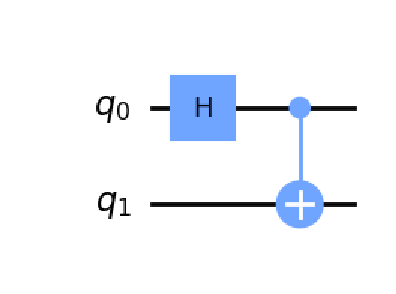
\includegraphics{bell_generate.eps}
    \caption{Bell状態の生成回路}
    \label{bell_kairo}
\end{figure}
 \begin{equation}\begin{split}
     \ket{00} \to \frac{\ket{0}+\ket{1}}{\sqrt{2}}\ket{0} \to \frac{1}{\sqrt{2}}(\ket{00}+\ket{11})
 \end{split} \end{equation}
CNOT以外のゲートが一粒子にのみ作用する点を考えると、量子もつれの生成は本質的にCNOTゲートに相当する。\\
\\
量子コンピュータの操作を最低限定義したが、このような量子コンピュータが果たして計算能力を本当に持つかは、自明な問題ではない。故に、まずは量子コンピュータの計算可能性について論じる。古典コンピュータにおいて、全ての演算は「NOT回路」と「AND回路」の組み合わせで分解される。量子計算においては、この「NOT回路」と「AND回路」はそれぞれXゲートとToffoliゲートに対応する。この時Toffoliゲートは２つの入力が両方1である場合のみ出力としてXゲートを対応させる回路である。このように、古典で全ての計算の元となる回路の対応物が量子コンピュータ上に存在するため、計算が効率的となるかはわからないが、量子コンピュータは、古典コンピュータで行う計算を少なくとも行うことが出来る。


\subsection{量子並列性とDeutsch-Jozsaのアルゴリズム}
以下で、量子コンピュータが古典コンピュータに比べて優位であることが示された例を述べる。\\
\\
古典コンピュータにはない明確な量子計算の特性として、複数の変数を同時に評価できる点が挙げられ、このことを「量子並列性」と呼ぶ。まずはアダマールゲートを用いることで複数の変数の重ね合わせとなる状態を作成できることを見る。
 \begin{equation}\begin{split}
     \hat{H}^{\otimes n}\ket{0}^{\otimes n} 
     &= (\frac{\ket{0}+\ket{1}}{\sqrt{2}})^{\otimes n} \\
     &= \frac{1}{\sqrt{2^{n}}} \Pi_{i} \sum_{x_{i}=0,1} \ket{x_{i}}\\
     &= \frac{1}{\sqrt{2^{n}}} \sum_{x=0}^{2^{n}-1} \ket{x}
 \end{split} \end{equation}
このため第１レジスタの数xを引数にとり第2レジスタにf(x)を渡すユニタリー演算子$U_{f}$が存在しそれを上の状態にかけた場合、状態の遷移は以下のように書ける。
\begin{equation}\begin{split}
    U_{f} (\frac{1}{\sqrt{2^{n}}} \sum_{x=0}^{2^{n}-1} \ket{x} \ket{0})
    = \frac{1}{\sqrt{2^{n}}} \sum_{x=0}^{2^{n}-1} \ket{x} \ket{f(x)}
\end{split} \end{equation}
これは確かに複数の変数についての関数の結果の重ね合わせに見えるが、一回の観測により出力が重ね合わせのうち1つの状態のみに表されるためこの操作だけでは量子並列性の要件を満たすことが出来ない。実際に「量子並列性」を示すためには、、何かしらの干渉効果を用いて、欲しい解の生成確率を高くする必要がある。本節では、「量子並列性」を示した最初の例である、Deutsch-Jozsaのアルゴリズムを紹介する。\\
\\
整数x=[0 , $2^{n}-1$ ]に対し、f(x)={0,1}を返す関数を考える。ただしこの時、f(x)はbalance型か定数型のどちらかであるとする。
この時、定数型はxの値に関わらず定数(0 or 1)をとるとし、blanced型はxの値に応じてランダムに半分が０、もう半分は１を返す関数とする。\\
\\
Deutsch-Jozsaのアルゴリズムは、f(x)は定数型かbalance型かどちらであるかをたった一回の計算で推定する、量子アルゴリズムである。\\
古典的には、関数がどちらであるかについて確実に回答を答えるためには$2^{\frac{n}{2}}+1$回の計算を行わなければならないが、このアルゴリズムによると、量子計算を用いると、１回の計算により確実に答えを出すことができる。これは明らかに量子優位性の例である。
\begin{setupbox}{Deutsch-Jozsaのアルゴリズム}
まず初期状態として、第１レジスタにn個、第２レジスタに1個の量子ビットを備え、$\ket{0}^{\otimes n}\ket{1}$を用意する。
次に第１レジスタ、第２レジスタに対して順次アダマールゲートを重ね合わせることで、以下の状態を生成する。
 \begin{equation}\begin{split}
     (\hat{H}\ket{0})^{\otimes n}\hat{H}\ket{1} 
     &= (\frac{\ket{0}+\ket{1}}{\sqrt{2}})^{\otimes n}(\frac{\ket{0}-\ket{1}}{\sqrt{2}})\\
     &= \frac{1}{\sqrt{2^{n}}}
     \sum_{i=0}^{2^{n}-1}\ket{i}(\frac{\ket{0}-\ket{1}}{\sqrt{2}})
 \end{split} \end{equation}
次に第１レジスタの変数に対してf(x)を計算し、その結果を第２レジスタにmod2で足し上げることが出来るようなユニタリー変換があったとして、それを$U_{f}$とする。これを量子状態にかけると、以下のようになる。(ただし$\oplus$はmod2で行う足し算であるとする)
  \begin{equation}\begin{split}
      U_{f}(\frac{1}{\sqrt{2^{n}}}\sum_{i=0}^{2^{n}-1}\ket{i}(\frac{\ket{0}-\ket{1}}{\sqrt{2}}))
      &=\frac{1}{\sqrt{2^{n}}}\sum_{i=0}^{2^{n}-1}\ket{i}(\frac{\ket{0\oplus f(i)}-\ket{1 \oplus f(i)}}{\sqrt{2}})\\
      &=\frac{1}{\sqrt{2^{n}}}\sum_{i=0}^{2^{n}-1}(-1)^{f(i)}\ket{i}(\frac{\ket{0}-\ket{1}}{\sqrt{2}})
  \end{split} \end{equation}
三段階目として第１レジスタにアダマールゲートをかける。(ただしi・jはi,jの２進数表記の各桁の係数の足し合わせである)
\begin{equation}\begin{split}
    \hat{H}^{\otimes n}(\sum_{i=0}^{2^{n}-1}(-1)^{f(i)}\ket{i})(\frac{\ket{0}-\ket{1}}{\sqrt{2}})
    =\frac{1}{2^{n}}  \sum_{j=0}^{2^{n}-1} \sum_{i=0}^{2^{n}-1}
    (-1)^{f(i)+i \cdot j}\ket{j}
\end{split} \end{equation}
この時仮にf(x)が定数型であるなら、j=0の振幅は$f(i)+i \cdot j = f(i) =const$となるため、$\frac{1}{2^{n}}\sum_{i=0}^{2^{n}-1}(-1)^{f(i)+i \cdot j} = (-1)^{f(i)}$である。全ての振幅の絶対値の２乗の和は1であるため、このことから、以下の関係が成立する。
\begin{equation}\begin{split}
\text{f(x)が定数型}\iff\text{第１レジスタの測定値が$\ket{0}$}
\end{split} \end{equation}
逆にbalance型の場合、j=0の振幅はi=[0,$2^{n}-1$]のうち半分が-1となり、もう半分が1となる。結局振幅が打ち消しあい０となる。このため、以下の関係が成立する。
\begin{equation}\begin{split}
\text{f(x)がbalanced型}\iff\text{第１レジスタの測定値が$\ket{0}$以外}
\end{split} \end{equation}
以上より、第１レジスタの値を観測すると、f(x)の形がわかるので、確かにアルゴリズムが実証された。
\end{setupbox}

\section{位相推定型アルゴリズム}
Deutsch-Jozsaのアルゴリズムで見たとおり、量子計算とはいうなれば正の確率、負の確率を持つ状態を重ね合わせを生成し、その確率をうまく操作することにより望んだ状態の振幅を上げることである。この節ではうまく重ね合わせが計算に組み込まれ、結果として古典に比べて指数関数的に計算速度を上げることに成功したアルゴリズムとして、位相推定を用いたアルゴリズムついて解説する。\\
\\
なお、はっきり言って、この節には直感的な描像が存在しない。ひたすら計算によるゴリ押しであることは最初に明記しておく。

\subsection{アダマールテスト}
位相推定問題とは、大雑把に言えば以下の問題である。
\begin{defbox}{位相推定問題}
位相推定問題とは、ユニタリオペレータUとその固有状態$\ket{\lambda}$が与えられた際、その固有ベクトルの「固有値」、もしくは「固有値の関数」を、量子計算を用いて推定できるか、という問題である。
\end{defbox}
例えば、量子力学の全てに通じる問題の一つとして、エネルギー準位を求めることが挙げられる。上記の問題はダイレクトにそれにつながるため、上記の問題を解くことは非常に重要である。\\
\\
この問題の一番シンプルな答えとして、「アダマールテスト」と呼ばれる手法で、ユニタリオペレータの固有値が求まることが知られている。アダマールテストは、図\ref{Hadamard_re},図\ref{Hadamard_im}の2種類の回路で構成される。\\
\begin{figure}[h]
    \centering
    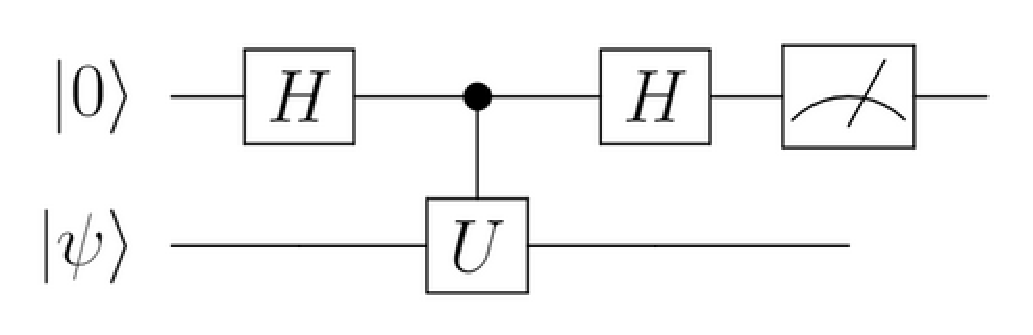
\includegraphics[height=3cm]{Hadamard_re.eps}
    \caption{アダマールテスト回路その１}
    \label{Hadamard_re}
\end{figure}
\begin{figure}[h]
    \centering
    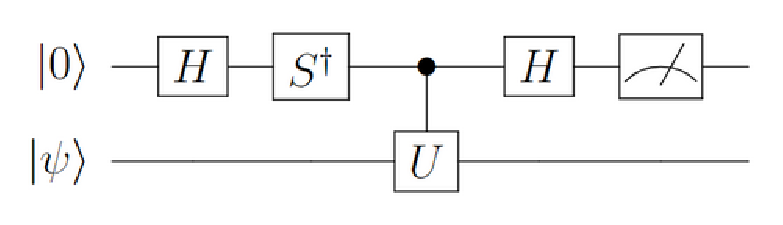
\includegraphics[height=3cm]{Hadamard_im.eps}
    \caption{アダマールテスト回路その２}
    \label{Hadamard_im}
\end{figure}
\\アダマールテストの入出力は以下である。
\begin{resultbox}{アダマールテスト}
アダマールテストは以下のような入出力の関係がある。\\
入力：ユニタリオペレータU, 初期状態$\ket{\phi}$ \\
出力：期待値$\bra{\phi}U\ket{\phi}$
\end{resultbox}
\begin{proofbox}
まず、\eqref{Hadamard_re}の回路の終状態は以下のようになる。
\begin{equation}\begin{split}
    \ket{final}=\frac{1}{2}(\ket{0}_{test}(\ket{\psi}+U\ket{\psi})
    +\ket{1}_{test}(\ket{\psi})-U\ket{\psi})
\end{split} \end{equation}
よって0,1が観測される確率はそれぞれ以下である。
\begin{align}
P^{re}_{0}&=\frac{1+Re(\bra{\psi}U\ket{\psi})}{2}\\
P^{re}_{1}&=\frac{1-Re(\bra{\psi}U\ket{\psi})}{2}
\end{align}
従って、オペレータの期待値の実部は$Re(\bra{\psi}U\ket{\psi})=P^{re}_{0}-P^{re}_{1}$である。\\
\\
次に、\eqref{Hadamard_re}の回路の終状態は以下のようになる。
\begin{equation}\begin{split}
     \ket{final}=\frac{1}{2}(\ket{0}_{test}(\ket{\psi}-iU\ket{\psi})
    +\ket{1}_{test}(\ket{\psi})+iU\ket{\psi})
\end{split} \end{equation}
よって0,1が観測される確率はそれぞれ以下の通りである。
\begin{align}
P^{im}_{0}&=\frac{1+Im(\bra{\psi}U\ket{\psi})}{2}\\
P^{im}_{1}&=\frac{1-Im(\bra{\psi}U\ket{\psi})}{2}
\end{align}
従って、オペレータの期待値の虚部は$Im(\bra{\psi}U\ket{\psi})=P^{im}_{0}-P^{im}_{1}$である。\\
\\
これらの結果を踏まえると、オペレータの期待値が以下のように与えられる。
\begin{align*}
\bra{\phi}U\ket{\phi}=P^{re}_{0}-P^{re}_{1}+i(P^{im}_{0}-P^{im}_{1})
\end{align*}
\end{proofbox}
仮にstateがUの固有状態$\ket{\lambda}$であるとすると、$\bra{\lambda}U\ket{\lambda}=\lambda$である。故に、アダマールテストは、位相推定問題の答えの一つである。\\
\\
またこの方法を用いて、エルミート演算子Hの固有値の近似値を求めることも可能である。
\begin{proofbox}
ユニタリ演算子Uを以下のように設定する。
\begin{align*}
U=exp(iHt)
\end{align*}
仮に$t <<1$とすると、期待値の式は以下のように書き換えられる。
\begin{align*}
<U>=1+i<H>t +O(t^{2})
\end{align*}
故に、エルミート共役の固有値を求めることが可能である。
\end{proofbox}

\subsection{位相推定アルゴリズム}
アダマールテストは確かに位相推定問題の一つの解法である。しかし、アダマールテストを用いて固有値を計算する際、以下のような問題点が存在。\\
\\
(1)量子コンピュータを実際に回す回数が非常に多い。\\
(2)確率の偏りを用いる性質上、厳密値にはどうあがいても到達できない。\\
\\
以上の問題を回避するため、位相推定問題のより効率のよいアルゴリズムが必要である。このための処方として導入されたのが、「量子フーリエ変換」であり、「Kitaevの位相推定アルゴリズム」である。
\subsubsection{量子フーリエ変換}
まずは最初に準備として、「量子フーリエ変換」という操作、及びその回路を定義する。
\begin{defbox}{量子フーリエ変換}
量子フーリエ変換のオペレータUは以下のような操作を行う回路として定義される。
\begin{equation}\begin{split}
    U_{QFT}\ket{n}=\sum_{m=1}^{N}\frac{1}{\sqrt{N}}exp(i\frac{2\pi m}{N}n) \ket{m}\equiv \ket{k} \label{furie}
\end{split} \end{equation}
\end{defbox}
この時、任意の重ね合わせ状態に対して量子フーリエ変換を作用させると、各状態の振幅は以下のような関係となることが分かる。
\begin{resultbox}{一般状態の量子フーリエ変換}
\begin{equation}\begin{split}
    U_{QFT}(\sum_{n=1}^{N} x_{n}\ket{n} )= \sum_{m=1}^{N} y_{m}\ket{m}\\
    y_{m} = \sum_{n=1}^{N} x_{n} \frac{1}{\sqrt{N}}exp(i\frac{2\pi n}{N}m)
\end{split} \end{equation}
このことにより、量子フーリエ変換は位相に対するフーリエ変換であると思うこともできる。
\end{resultbox}
また、自然数を量子フーリエ変換した際の結果を明記することは、量子コンピュータ上に実際に量子フーリエ変換を実装する際に非常に重要である。
\begin{resultbox}{自然数jの量子フーリエ変換}
\begin{equation}\begin{split}
   U_{QFT}\ket{j} 
	= \frac{1}{2^{m/2}} (\ket{0}+e^{i2\pi 0.j_{0}} \ket{1})
                                  (\ket{0}+e^{i2\pi 0.j_{1}j_{0}} \ket{1})
                                \cdots(\ket{0}+e^{i2\pi 0.j_{m-1}\cdots j_{0}} \ket{1})
\end{split} \end{equation}
ただし、$0.j_{1}j_{2}\cdots$は２進数小数点表現である。
\end{resultbox}
\begin{proofbox}
単に、量子フーリエ変換の定義式に$n=j,N=2^{m}$を代入すればよい。
\begin{equation}\begin{split}
    U_{QFT}\ket{j}
    &= \sum_{l=0}^{2^{m}-1}\frac{1}{\sqrt{2^{m}}}exp(i\frac{2\pi j}{2^{m}}l) \ket{l}\\
    &= \sum_{l=0}^{2^{m}-1}\frac{1}{\sqrt{2^{m}}} exp(i\frac{2\pi j}{2^{m}}\sum_{k=0}^{m-1}l_{k}2^{k})\ket{l_{m-1}\cdots l_{0}}\\
    &= \sum_{l_{m-1}=0,1} \cdots \sum_{l_{0}=0,1}  \frac{1}{\sqrt{2^{m}}} \Pi_{k=0}^{m-1} exp(i\frac{2\pi j}{2^{m}}l_{k}2^{k})\ket{l_{m-1}\cdots l_{0}}\\
    &= \Pi_{k=0}^{m-1} \sum_{l_{k}=0,1} \frac{1}{\sqrt{2}}
    exp(i\frac{2\pi j}{2^{m}}l_{k}2^{k})\ket{l_{k}}\\
    &= \Pi_{k=0}^{m-1} \frac{\ket{0}+exp(i2\pi j 2^{k-m})\ket{1}}{\sqrt{2}}\\
    &=\frac{1}{2^{m/2}} (\ket{0}+e^{i2\pi 0.j_{0}} \ket{1})
                                  (\ket{0}+e^{i2\pi 0.j_{1}j_{0}} \ket{1})
                                \cdots(\ket{0}+e^{i2\pi 0.j_{m-1}\cdots j_{0}} \ket{1})
\end{split} \end{equation}
\end{proofbox}
この表式により、量子コンピュータにおいて量子フーリエ変換を実際にどう実装すればいいかが理解できる。回路図は、以下の通りである。\\
\begin{figure}[h]
    \centering
    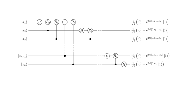
\includegraphics[height=5cm]{Q_fourier_nqubits.eps}
    \caption{量子フーリエ変換の回路\\(引用：https://commons.wikimedia.org/wiki/File:QuantumPhaseEstimationCircuit.eps)}
    \label{fig_QFT}
\end{figure}
\\この時、$R_{k}$ゲートは以下である。
\begin{equation}\begin{split}
    R_{k}=\mqty(1 & 0 \\ 0 & e^{i \frac{2\pi}{2^{k}}})
\end{split} \end{equation}
\\
以下、n量子ビットの量子フーリエ変換の計算量を見積もる。\\
まず、量子コンピュータ上でのアダマールゲートと$R_{k}$ゲートの作用回数は、回路図\ref{fig_furie}より、$n+n-1\cdots 1 = \frac{n(n+1)}{2}$回掛ければよい。\\
次にCNOTゲートの作用回数を考える。この際、実機での実装を考えると、CNOTは隣接したビット間にしか作用できない点に注意が必要である。離れたゲートを作用させる量子フーリエ変換の形に持っていくためには、SWAPゲートを用いて順番を入れ替える必要があるが、その回数は高々$\frac{n}{2}$回程度であることを考えると、計算回数は精々$n^{2}$程度となる。\\
これら全てを踏まえると、量子フーリエ変換の実装において必要なゲート数は、$O(n^{4})$程度である。\\
\\
古典における$2^{n}$個の要素を離散フーリエ変換することは、純粋に考えると$2^{n}\times2^{n}$個の行列要素をすべて計算する必要があるため、単純に考えた場合計算に必要な時間は$O(2^{n})$となり、指数関数的に多くの処理が必要となる。また、現状考えられている最速のフーリエ変換の導出手法である高速フーリエ変換であっても、っその処理速度は$O(n2^{n})$となることが知られている。このことを踏まえると、量子フーリエ変換は古典シミュレーションに対して指数的な有意性を与える。\\
\\
では、量子フーリエ変換は古典コンピュータにおける離散フーリエ変換の完全な上位互換となりうるか？答えは否である。これは量子フーリエ変換を行った\eqref{furie}を見ると理解できるように、全て振幅に対して定義する操作であるためフーリエ変換の波数ベクトルの成分そのものを読み取ることが出来ない。このことから、例えば古典において音声データを古典コンピュータに代わり量子コンピュータでフーリエ変換する、といった処理はできない。\\
\\
次に、量子フーリエ変換の逆操作である、「量子逆フーリエ変換」に関して述べる。量子逆フーリエ変換は以下のように定義される変換である。ユニタリー演算子としては$U_{FT}^{\dagger}$と記述する。
\begin{equation}\begin{split}
 U_{QFT}^{\dagger}\ket{k} = \ket{n} 
    =\sum_{l=1}^{N}\frac{1}{\sqrt{N}}exp(-i\frac{2\pi l}{N}k) \ket{l} \label{furie_two}
\end{split} \end{equation}
また量子フーリエ変換で作用させる各ゲートはそれを打ち消すゲートがほぼ自明であるため、量子フーリエ変換が導出できるなら量子逆フーリエ変換の回路は簡単に導出できる。\\

\subsubsection{Kitaevの位相推定アルゴリズム}
直前のセクションで導入した「量子逆フーリエ変換」が、実は位相推定問題において本質的な役割を果たす。以下では、この量子フーリエ変換を用いた位相推定アルゴリズムの処方である、「Kitaevのアルゴリズム」を導入する。\\
\\
まずは簡単のため、ユニタリーゲートU,及び固有状態$\ket{\phi_{u}}$が準備でき、なおかつ固有値$exp(i2\pi u)$のuの値が、n量子ビットを用いて以下のように正確に表現できた場合を考える。
\begin{equation}\begin{split}
    u=\sum_{i=0}^{n-1} u_{i}2^{i-n}\: \text{(ただし、$u_{i}=0,1$のいずれか)} \label{u}
\end{split} \end{equation}
その場合、位相推定アルゴリズムの回路は\eqref{fig_isou}のように書ける。\\
\begin{figure}[h]
    \centering
    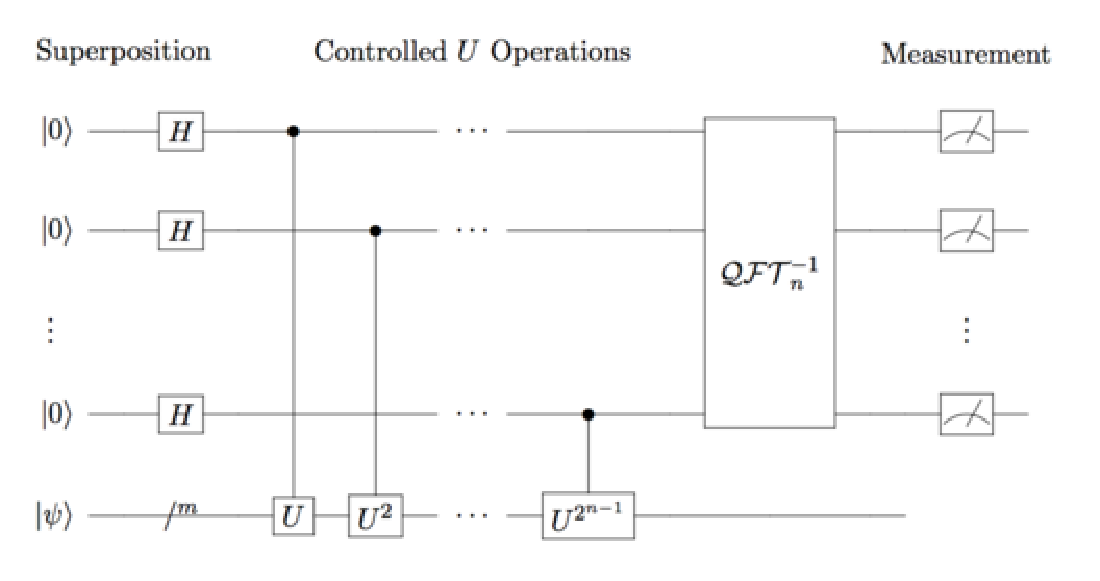
\includegraphics[height=5cm]{QuantumPhaseEstimationCircuit.eps}
    \caption{位相推定アルゴリズムの模式図\\(引用：https://commons.wikimedia.org/wiki/File:QuantumPhaseEstimationCircuit.eps)}
    \label{fig_isou}
\end{figure}
\\この位相推定アルゴリズムでは、出力と入力は以下のようになる。
\begin{resultbox}{位相推定アルゴリズム}
入力：ユニタリオペレータU, 初期状態$\ket{\phi}\otimes\ket{0}^{\otimes n}$ \\
出力：$\ket{\phi}\ket{u\times2^{n}}$
\end{resultbox}
\begin{proofbox}
Figure.\ref{fig_isou}の回路図を、式変形で追っていくことで示せる。
\begin{equation}\begin{split}\label{isou2}
    & \ket{0}\ket{\phi_{u}}\;\text{(初期状態)}\\
    & \to (\frac{\ket{0}+\ket{1}}{\sqrt{2}})^{\otimes n}\ket{\phi_{u}}\;
    \text{ (第１レジスタにアダマールゲートの作用)}\\
    & \to  
    (\frac{\ket{0}+\ket{1}}{\sqrt{2}})^{\otimes n-1} (\frac{\ket{0}+exp(i2\pi 2^{0}u)\ket{1})}{\sqrt{2}} \ket{\phi_{u}}\;
    \text{($U^{2^{0}}$ゲートの作用)}\\
    \;\;\;\;\;\;\;\;\vdots \\
    & \to \Pi_{j=0}^{n-1} (\frac{\ket{0}+exp(i2\pi 2^{n-j} u)\ket{1}}{\sqrt{2}})
    \ket{\phi_{u}}\:\text{(逆フーリエ変換以外全てのゲートの適応)} \\
    &=\frac{1}{2^{n/2}} (\ket{0}+e^{i2\pi 0.u_{0}} \ket{1})
                                  (\ket{0}+e^{i2\pi 0.u_{1}u_{0}} \ket{1})
                                \cdots(\ket{0}+e^{i2\pi 0.u_{n-1}\cdots u_{0}} \ket{1})\\
    &\to \ket{u\times2^{n}}\ket{\phi_{u}} \:\text{(逆フーリエ変換の適用)}
\end{split} \end{equation}
よって固有状態及び固有値が適切に定義できた場合、第１レジスタの観測によりその固有値が確実に読み出せることとなることががわかる。
\end{proofbox}
次に、より一般のユニタリオペレータの位相推定について考える。\\
ユニタリー演算子Uの固有値は一般的に$exp(i2\pi u)$の形で書けるが、uの値は実数である。その場合の固有値は\eqref{isou2}の式変形が適応できないことがわかる。では、この位相推定アルゴリズムは、特殊なクラスにだけ適用できる処方だろうか？実は、上記の量子位相推定アルゴリズムは、正確な固有値を読みだすことは出来ずとも、近似値を読みだすことができるアルゴリズムであることが、具体的な計算から理解できる。\\
\begin{resultbox}{一般の位相推定アルゴリズム}
位相推定アルゴリズムを用いると、一般のユニタリーオペレータでも、固有値の近似値が確率的に読み出すことが出来、また、その確率に下限値を与えることが出来る。
\end{resultbox}
\begin{proofbox}
先ほどの例で、uが必ずしもNビットを用いて正確に記述できないとする。この場合、\eqref{isou}から\eqref{isou2}への式変形が出来ないため、\eqref{isou}式から直接逆フーリエ変換の式を計算する。そのため、まず\eqref{isou}の式変形から行う。
\begin{equation}\begin{split}
    \eqref{isou}=&\Pi_{j=0}^{n-1} (\frac{\ket{0}+exp(i2\pi 2^{n-j} u)\ket{1}}{\sqrt{2}})
    \ket{\phi_{u}}\\
    &=\sum_{k_{n-1}=0,1} \cdots \sum_{k_{0}=0,1} \frac{1}{\sqrt{2^{n}}}exp(i2\pi u(k_{n-1}2^{n-1}+\cdots+k_{0}2^{0}))\\
    &\ket{k_{n-1}}\cdots\ket{k_{0}}\ket{\phi_{u}} \\
    &=\frac{1}{\sqrt{2^{n}}}\sum_{k=0}^{2^{n}-1} exp(i2\pi ku)\ket{k}\ket{\phi_{u}}
\end{split} \end{equation}
このため、\eqref{isou}の逆フーリエ変換は\eqref{furie_two}の式を$\ket{k}$に対して行うと最終的な状態は以下のようになる。
\begin{equation}\begin{split}
    \frac{1}{2^{n}}\sum_{k,l=0}^{2^{n}-1}exp(i2\pi k(u-\frac{l}{2^{n}}))\ket{l}\ket{\phi_{u}}
\end{split} \end{equation}
よって最終状態は$\ket{0}\cdots\ket{2^{n}-1}$の重ね合わせ状態となる。\\
\\
以後第１レジスタのみを考え、各確率振幅に対して評価を行うことを考える。まずuの小数点第n桁までの近似値を$\bar{u}$(ただし$u\geq\bar{u}$)とし、残りの部分を$\delta$とする。この時、$0 \leq \delta <2^{-n}$といえる。この時$\ket{2^{n}\times \bar{u}+v(mod\:N)}$に対応する振幅を$a_{v}$とすると、
\begin{equation}\begin{split}
a_{v}&=\frac{1}{2^{n}}\sum_{k=0}^{2^{n}-1} exp(i2\pi k(u-\frac{2^{n}\times \bar{u}+v}{2^{n}}))\\
     &=\frac{1}{2^{n}}\sum_{k=0}^{2^{n}-1} exp(i2\pi k(\delta-\frac{v}{2^{n}}))\\
     &=\frac{1}{2^{n}}\frac{1-exp(i2\pi (2^{n}\delta-v))}{1-exp(i2\pi (\delta-\frac{v}{2^{n}}))}
\end{split} \end{equation}
これを用いてuの近似値がどの程度の精度で読み出せるかを評価する。\\
まず、許容誤差e(ただし、eは読み取ったビットの状態で読み取ったものがどれだけ離れたかを評価する数字なので、整数であるとする)でuを推定することを考える際、観測値が許容誤差を超える確率$P(|2^{n}\times u - l|>e)$は以下のように考えることが出来る。(この時、のちの議論のことを考えてvのとりうる範囲を$-2^{n-1} < v\leq 2^{n-1}$と記述する。これはmod$2^{n}$の下で$0\leq v \leq 2^{n}-1$と等価である)
\begin{equation}\begin{split}
    P(|2^{n}\times u - l|>e) = (\sum_{v=-2^{n-1}+1}^{-(e+1)} +\sum_{v=e+1}^{2^{n-1}} ) |a_{v}|^{2}
\end{split} \end{equation}
複素平面における幾何的な考察により$|1+exp(i\theta)| \leq 2$、かつ$(-\pi < \theta \leq \pi)$においては$|1+exp(i\theta)|\geq \frac{2|\theta|}{\pi}$が成り立つことがわかり、また$-\frac{1}{2}\leq \delta-\frac{v}{2^{n}} \leq \frac{1}{2}$であるため上の不等式が両方成立し、$a_{v}$に対して以下の評価式が成立する。
\begin{equation}\begin{split}
    |a_{v}| \leq \frac{1}{2^{n+1}} |\frac{1}{\delta-\frac{v}{2^{n}}}|
\end{split} \end{equation}
このため、$P(|2^{n}\times u - l|>e)$は以下のように評価できる。
\begin{equation}\begin{split}
    P(|2^{n}\times u - l|>e) 
    &\leq (\sum_{v=-2^{n-1}+1}^{-(e+1)} +\sum_{v=e+1}^{2^{n-1}} ) 
    \frac{1}{4} \frac{1}{(2^{n}\delta-v)^{2}} \\
    &\leq \frac{1}{4}
    \sum_{v=-2^{n-1}+1}^{-(e+1)} \frac{1}{v^{2}}
    +\sum_{v=e+1}^{2^{n-1}} \frac{1}{(v-1)^{2}}\:(0\leq 2^{n}\delta <1)\\ 
    &\leq \frac{1}{4}
    \sum_{v=-2^{n-1}+1}^{-e} \frac{1}{v^{2}}
    +\sum_{v=e+1}^{2^{n-1}} \frac{1}{(v-1)^{2}} \:\text{(和の範囲の拡大)}\\
    &=\frac{1}{2}\sum_{v=e}^{2^{n}-1} \frac{1}{v^{2}}\\
    &\leq \frac{1}{2} \int_{e-1}^{2^{n}-1} dv \frac{1}{v^{2}}\\
    &\leq \frac{1}{2(e-1)}
\end{split} \end{equation}
これにより、uの値を、許容誤差eの下で推定できる確率は、最低$1-\frac{1}{2(e-1)}$となる。
\end{proofbox}
逆に、固有値を制度$2^{-t}$桁まで一致させる確率を求めるには、$e=2^{n-t}-1$と取ることにより成功確率は$1-\frac{1}{2(2^{n-t}-2)}$となることが示せるので、許容誤差と望む成功確率から用意すべきビット数を割り出すことが出来る。許容誤差$2^{-t}$までで成功確率$1-\frac{1}{e}$で得るために欲しいビット数nは$n=t+log_[2](2+\frac{1}{2\epsilon})$である。\\
\\
以上により、一般的なユニタリーゲートの場合でも固有値の近似値を高い確率で読み出せることは理解できた。物理のダイナミクスを考える際にはその時に固有状態が観測値により変化しないという部分も重要になる。これにより、位相推定アルゴリズムを用いることで状態を変化させずにエネルギー固有値を読み出すことが出来る。このように、標的ビットが状態を変化させず制御ビットに位相を返す現象を、「位相キックバック」と呼ぶ。\\
\\
また、仮に第２レジスタの状態が固有状態ではなく、その重ね合わせならどうだろうか？これはユニタリーゲートが線形であることを用いると位相推定アルゴリズムの議論が線形性よりそのまま各固有状態に対して適応できる為、位相推定アルゴリズムを用いた場合最終的な第１レジスタの状態は固有値の重ね合わせとなるので、最終的には固有値のうちの１つが計算されることになる。またその時、第２レジスタは観測された固有値の固有状態に収束する。\\
\\
最後に気を付けるべきことは、この位相推定アルゴリズムはユニタリーゲートとして$U^{2^{n-1}}$ゲートをかける必要があることである。これを遂行する素朴な方法は単純にユニタリーゲートを所要回数かけることだが、そうすると位相推定アルゴリズムはビット数に対して指数関数的な回数の処理が必要となる。従って、ゲートを縮約できる場合のみ、量子計算が優位に働くことを留意しなければならない。\\

\subsection{位数発見と素因数分解}
位相発見アルゴリズム自体の使い方は様々であるが、そのうちの一つが恐らく最も量子計算で有名であろうアルゴリズムである素因数分解のアルゴリズムである、shorのアルゴリズムであろう。また、その問題は本論文で扱う範囲においては位数発見問題という問題と等価であり、この位数発見問題が量子コンピュータがどういった問題で優位性を発揮するかという観点でより一般的な知見を与える。\\
\\
まずここでいう位数は、xとNという互いに素な２整数(x<N)を考えた際、以下を満たす最小の整数rとして定義される。(ただし、整数A,Bに対してA(mod N)は整数をNで割った余りを指し、A=B(mod N)は整数A,BをNで割った余りが等しいことを指す)
 \begin{equation}\begin{split}
     x^{r} = 1 \:(mod\:N)
 \end{split} \end{equation}
位数発見問題とは、条件を満たすある整数x,Nが与えられた際に、rを決めるような問題である。(このようなrは任意のx,Nに対して存在し、必ずNよりも小さいことが分かっている。証明方法としてはmod Nがとりうる数字は1からN-1であるためrが2(N-1)となるまでの間で$x^{r}(mod\:N)$は最低１回は同じ数字をとり、その間の数字の数はN-1個以下であるためmod計算の公式より示すことが出来る)\\
\\
この問題を決定するのに必要なビット数O(L)(Lはx,r,Nの中で最大であるNを表現するために必要なビット数L=[logN]に対して多項式時間でこの位数を決めるアルゴリズムは現状見つかっていないため、この問題は解くのが難しい問題であると考えられている。しかし、この問題に対して量子コンピュータは位相推定アルゴリズムを用いることにより、古典よりも効果的な方法で問題が解けることがわかっている。\\
\\
位数推定アルゴリズムというのは、状態yに対し法Nの下でNに対してxをかけるような状態に変化させるユニタリーゲート$U_{x}$の固有値問題に帰着することが出来る。(ただし、この時Nより大きいyに関してはユニタリーゲートは効果を発揮せず、yのままであるとする)
 \begin{equation}\begin{split}
     U_{x}\ket{y} = \ket{xy \:(mod \:N)} \label{Uxn}
 \end{split} \end{equation}
 この時、仮にxのNに対する位数がrであるなら、ユニタリーゲートの固有状態は$0\leq s <N$を用いて以下のように書けることが、簡単な計算により示すことが出来る。
 \begin{equation}\begin{split}
     \ket{u_{s}} &= \frac{1}{\sqrt{r}}\sum_{j=0} ^{r-1}exp(-\frac{i2\pi s j}{r}) \ket{x^{j}}\\
     U_{x}\ket{u_{s}}
     &=\frac{1}{\sqrt{r}}exp(\frac{i2\pi s}{r}) \sum_{j=0} ^{r-1} 
                       exp(-\frac{i2\pi s (j+1)}{r}) \ket{x^{j+1}}\\
     &=exp(\frac{i2\pi s}{r}) \frac{1}{\sqrt{r}}\sum_{j=0} ^{r-1} 
     exp(-\frac{i2\pi s j}{r}) \ket{x^{j}}\\
     &=exp(-\frac{i2\pi s}{r}) \ket{u_{s}}
 \end{split} \end{equation}
この時、位数がrであると仮定したときに成り立つ式$exp(-\frac{i2\pi s (j+1)}{r})\ket{x^{j+1} }|_{j=r-1}= exp(-\frac{i2\pi s \times0}{r})\ket{x^{0}}$が成り立つことを式変形で用いた。このことにより位相推定から$\frac{s}{r}$を読みだすことが出来る。取り出した位相からどのようにrを計算するかの議論は後にするとして、まずは位相推定の方面からこのアルゴリズムを実現しうるかを考える。\\
\\
位相推定は固有状態を用意できた場合にその固有値を読みだすことが出来るアルゴリズムである。このことは固有状態が完全系をなす場合は取りだす位相が固有値のうちのどれかになるため取り出す値そのものは固有値であるが、位相推定の$U_{x}$は$2^{L}$個の独立な状態ベクトルの中で$\ket{u_{s}}$はN個のみ存在するため、取り出した数値が果たして本当に位相となっているかが全く自明ではない。しかも、$\ket{u_{s}}$を用意するためには$j=0 \cdots r-1$に対する$\ket{x^{j}}$を用意しなければならないが、それが用意できるということは結局用意する過程で位数発見が出来てしまっているため、位相発見を考えるために予め位数発見をするという状況に陥ってしまい、位相推定を行う意味がない。しかし、以下のような関係式を満たせることが証明できるので、この式の存在により位数発見の固有状態の線形結合が自明な状態であることが導ける。
 \begin{equation}\begin{split}
     \frac{1}{\sqrt{r}}\sum_{s=0}^{r-1} exp(\frac{i2\pi s k}{r})\ket{u_{s}}
     = \ket{x^{k}\:(mod\:N)}
 \end{split} \end{equation}
よってk=rと置いた場合に$x^{r}=1\:(mod\:N)$よりk=rでの上式の左辺は$\ket{1}$という自明な式となる。この式は$\ket{u_{s}}$の定義を用いると以下のように簡単に証明できる。
\begin{equation}\begin{split}
    \frac{1}{\sqrt{r}}\sum_{s=0}^{r-1} exp(\frac{i2\pi s k}{r})\ket{u_{s}}
    &= \frac{1}{r}\sum_{s=0}^{r-1} \sum_{j=0} ^{r-1}
      exp(-\frac{i2\pi s j}{r}) exp(\frac{i2\pi s k}{r})\ket{x^{j}\:(mod\:N)}\\
    &=\sum_{j=0} ^{r-1} \delta_{k-j,0} \ket{x^{j}\:(mod\:N)}\\
    &=\ket{x^{k}\:(mod\:N)}
\end{split} \end{equation}
公式の証明に$\sum_{s=0}^{r-1}exp(\frac{i2\pi s (k-j)}{r})=r\delta_{k-j,0}$を用いた。これにより、最終的に以下の式が成立する。
\begin{equation}\begin{split}
    \sum_{s=0}^{r-1} \ket{u_{s}}=\ket{1\:(mod\:N)}
\end{split} \end{equation}
この関係式により、rの詳細に触れずとも$U_{x}$の固有状態の重ね合わせが実現できることがわかったので、量子位相推定により固有値を取り出せることがわかった。\\
次にユニタリーゲートの縮約について考える。基本的な考え方としては位相推定におけるユニタリーゲートの計算が
$\ket{z}\ket{y} \to \ket{z}\ket{x^{z}y}$の形で実装されることを用いる。これを計算するためには第３レジスタを定義してまず$x^{2}$を計算し、その値を第２レジスタに乗ずる。この後に第３レジスタを乗ずる計算を行い、その値を第２レジスタにかける。これをN回行った後に、最終的に第３レジスタを初期化する。この操作により、「仮に第３レジスタの数を第２レジスタに乗ずる場合にその操作の数が第３レジスタの数字に関わらない」のであれば$x^{2n}$のみを計算してそれを乗ずる操作のみでユニタリーゲートの操作が全てかけるので、Nまでの値を2乗するのに必要な操作量を筆算と同じだと仮定してO($L^{2}$),掛け算を行う回数がO(L)であり、ユニタリーゲートの全体の計算量は$O(L^{3})$となる。\\
\\
位相推定により固有値$\frac{s}{r}$を取り出すことが出来るが、一般にこれは有限の小数点で打ち切られる近似値φであることが位相推定の考察より理解できる。従って、この近似値から分数を求めることで実際のrを計算できるが、そもそも推定して得られた分数は本当に$\frac{s}{r}$となるのか？付録連分数アルゴリズムの議論によると、その問題は解決できることが示せる。\\
\\
仮に位相推定アルゴリズムに対して用意するビット数を$n=2L+1+log_{2}(2+\frac{1}{2\epsilon})$であるとすると、$1-\frac{1}{e}$の確率で$|\phi -\frac{s}{r}|\leq \frac{1}{2r^{2}}$を満たす$\phi$が求まることがわかる。\\
\\
最後の問題はこの$\frac{s}{r}$がrを再現するか否かである。これは２つ注意すべきことがあり、一つは位相推定アルゴリズムにおいて$\frac{s}{r}$が量子ビットで書けない場合の補正である。これに関しては位相推定の欄で議論をした通り、。もう一つは元々取り出そうとしていたrとsが互いに素ではない場合である。このことは根源的には避けようがないが、以下のような手続きで一定確率以上でrが構成できることが証明できる。\\
\\
 まず、連分数アルゴリズムまでの流れを２回連続で行うことを考える。この時sが0からr-1の間でランダムに出てくるので、「２回出てきたsが互いに素であるなら」どちらかのsがrの因数を含んでいたとしても、もう片方はその因数を含んでいないので出力されたrの最小公倍数を考えることにより真のrが取り出せることがわかる。この２回が互いに素である確率はr以下の素数をqとすると以下のように書ける。
\begin{equation}\begin{split}
    1-\sum_{q}(\text{$s_{1}$がqで割れる確率})\times (\text{$s_{2}$がqで割れる確率})
\end{split} \end{equation}
素数qで割る際に余りが0からq-1であるからランダムで選ばれた$s_{1}$がqで割れる確率は$\frac{1}{q}$であることがわかる。rのあまりの周期が1から始まって0で終わることを留意すると、
\begin{equation}\begin{split}
    1 - \sum_{q} (\text{$s_{1}$がqで割れる確率}) \times (\text{$s_{2}$がqで割れる確率})
    \geq 1 - \sum_{q} \frac{1}{q^{2}}
\end{split} \end{equation}
区分求積法を用いてこの式を評価すると、最終的に適切な位数rが求まる確率に以下のような下限が存在することがわかる。

\begin{equation}\begin{split}
    (\text{rが適切な位数である確率}) 
    \geq 1 - \sum_{q} \frac{1}{q^{2}}
    > 1 - \frac{1}{4} +\int_{2}^{\infty} dr \frac{1}{r^{2}}
    = \frac{1}{4}
\end{split} \end{equation}
以上の結果をまとめると、位数発見アルゴリズムは以下のような手続きで考えられる。
\begin{itembox}[l]{位数発見アルゴリズム}
用意するもの：第一レジスタに$n=2L+1+log(2+\frac{1}{2\epsilon})$、第2レジスタにL個の量子ビット、及び\eqref{Uxn}を満たすようなユニタリーゲート$U_{x}$\\
1.初期状態      $\ket{0}\ket{1}$ \\
2.第１レジスタのすべてにアダマールゲートを作用し、重ね合わせの生成 $\sum_{j=1}^{N}\ket{j}\ket{1}$\\
3.$U_{x}$の適用 $\sum_{j=1}^{2^{t}-1}\ket{j}\ket{x^{j}} = \sum_{j=1}^{2^{t}-1} \sum_{s=0}^{r-1} exp(\frac{i2\pi s j}{r})\ket{j}\ket{u_{s}}$\\
4.第１レジスタにフーリエ逆変換の適応  $\sum_{s=0}^{r-1}\ket{\frac{s}{r}}\ket{u_{s}}$\\
5.第１レジスタの測定及び連分数アルゴリズムの適用、及び検証\\
出力：xの位数r\\
成功確率：$\geq \frac{1}{4} \times 1-\frac{1}{e}$\\
所要計算回数：O($L^{3}$)\\
\end{itembox}
この位数発見アルゴリズムが素因数分解と同等の問題であるとみなせる理由は以下の2つの定理が成り立つ点である。
1.NをLビットの合成数であるとし、xを$1\leq x \leq N-1$かつ$x^{2}=1\:(mod\:N)$の自明でない解である($x\neq 1,N-1$)とし、a,bの約数をgcd(a,b)と記述すると、gcd(x-1,N)とgcd(x+1,N)の少なくとも一方はNの素因数であること。
2.Nを奇数である正の合成数だとする。xが$1\leq x \leq N-1$のうちからランダムに一つ選ばれて、Nと互いに素であったとする。また、xのNを法とする場合の位数がrであったとすると、
\begin{equation}\begin{split}
    p(\text{rが偶数、かつ}x^{r} \neq 1\;(mod\;N)) \geq 1 - \frac{1}{2^{m-1}} 
\end{split} \end{equation}
この２つの定理により、仮に位数発見アルゴリズムで位数を見つけることができた場合、高い確率で素因数を計算することができる。

\subsection{一般化(隠れ部分群問題への拡張)}
位数発見問題はNを法とする乗法に対する周期を発見する問題であったと考えることが出来る。これを考えると量子フーリエ変換を用いた一連の手続きはある種の周期発展問題に対応できることが期待される。このことは群の用語を用いるとより一般的に「隠れ部分群問題」として議論することが可能である。
\begin{itembox}[l]{隠れ部分群問題}
有限に生成された群をＧとし、fをGから有限集合Xに移す関数であるとする。また、f(G)の写像先はGの部分群Kの剰余類上で一定であり、逆に剰余類間では異なるとする。この時、集合X上で適切な二進数演算$\oplus$が与えられたとき、またユニタリー変換$U\ket{g}\ket{h}=\ket{g}\ket{h\oplus f(g)}$が与えられたとき、部分群Kを表現できる生成元の集合(生成集合)を見いだす問題
\end{itembox}
隠れ部分群問題に対して特に群Gが可換である場合、位数発見アルゴリズムとほぼ同じ考え方で理解することが出来ることがわかる。そのことを理解するため、群の観点からこの問題をどう議論できるかを見る。\\
まず、隠れ部分群問題を量子計算の議論に持ち込む際に重要となる、可換群に対するいくつかの性質を先に述べておく。以下、群の位数(要素の数)を|G|であるとする。\\
1.可換群の既約表現は必ず１次元となる。\\
2.可換群は整数におけるGを法とする加法群と同型(つまり、可換群の要素は整数と対応させることが出来る)\\
3.群の表現では共役類の数と等しい数の非同値かつ既約な表現の方法が存在する。(可換群の場合、群の共役類は群になるため、表現の数は群の要素数と等しい)\\
このことを利用して、群Gを有限の整数集合Xに写像する関数fに関するフーリエ変換を以下のように定義する。
\begin{equation}\begin{split}
    \tilde{f}(\rho) = \sum_{g \in G} f(g) \rho (g)
\end{split} \end{equation}
これは実数のフーリエ変換が実空間と波数空間を直交性のある形で1:1対応させていることに対し、3の性質を用いて可換群を同数である表現の仕方と対応させている(直交性は大直行定理により保証される)。また1,2の性質を考えると可換群の表現の元は$l=[0,|G|-1]$を用いて、以下のように表すことが出来る。
\begin{equation}\begin{split}
    \rho_{h} (g) = exp(i2 \pi \frac{gl}{|G|})
\end{split} \end{equation}
よって可換群の要素gを加法の有限整数群に対応させた場合にそのフーリエ変換は以下のように書ける。
\begin{equation}\begin{split}
    \tilde{f}(l) = \sum_{g=0}^{|G|-1} f(g) exp(-i2 \pi \frac{gl}{|G|})
\end{split} \end{equation}
次に関数に部分群Hが隠れている、つまり$f(g \circ H) = f(g)$である場合、群のフーリエ変換の要素がとびとびとなることを見る。例えば実数xを実数に写像させる関数f(x) において隠れ部分群として$\{0,a,2a \cdots \}$が存在するとすると、f(x)=f(x+a)となり、フーリエ変換を考えた際にとびとびの値以外全て０になるため、部分群による周期性の存在はフーリエ変換の係数に強い制限を与える。隠れ部分群Hの要素をhであるとすると、g=h+g'と書けるため、群における隠れ部分群がある関数のフーリエ変換は以下のように書ける。
\begin{equation}\begin{split}
    \tilde{f}(l)
    &=\sum_{g=0}^{|G|-1} f(g) exp(-i2 \pi \frac{gl}{|G|})\\
    &=\sum_{h \in H} \sum_{g'=1}^{h-1} exp(-i2 \pi \frac{(g'+h)l}{|G|})f(g'+h)\\
    &=\sum_{g'=1}^{h-1} f(g') exp(i2 \pi \frac{g'l}{|G|})\sum_{h \in H} exp(-i2 \pi \frac{hl}{|G|})
\end{split} \end{equation}
このため$hl \in |G|Z$の形ではない限り$\sum_{h \in H} exp(-i2 \pi \frac{hl}{|G|})$は位相同士で打ち消しあうため、０の振幅をとる。これによりlの値が制限され、lの値が具体的に求まれば$hl \in |G|Z$によりhもまた決まることが出来る。そのため、隠れ部分群を決定することが出来る。この考え方を用いて隠れ部分群の発見問題は以下のような手続きで解くことが出来る。
\begin{itembox}[l]{隠れ部分群問題のアルゴリズム}
用意するもの：可換群及び有限集合f(g)を表現できるL個の量子ビット、及び$U_{f}\ket{g}\ket{h}=\ket{g}\ket{h \oplus f(g)}$を満たすブラックボックス$U_{f}$(ただし$U_{f}$は群の表現にならない整数に対しては何も操作を行わないものとする) \\
1.可換群Gを積表を用いて整数に変換させる。\\
2.初期状態： $\ket{0}\ket{0}$\\
3.第１レジスタにアダマールゲートをかける：$\sum_{g=0}^{2^{n}-1}\ket{g}\ket{0}$\\
4.ブラックボックスの適応：$\sum_{g=0}^{2^{n}-1}\ket{g}\ket{f(g)}=\sum_{g=0}^{2^{n}-1}
\sum_{l \in G}exp(i2\pi \frac{gl}{|G|})\ket{g}\ket{\tilde{f}(l)}$\\
5.第一レジスタの逆フーリエ変換：$\sum_{l \in G} \ket{\frac{\tilde{l}}{|G|}}\ket{\tilde{f}(l)}$\\
6.連分数アルゴリズム：lを推定\\
仮に隠れ部分群が存在するなら$\sum_{h \in H} exp(i2 \pi \frac{hl}{|G|})$が0となるlが存在するため、それにより出てくるlに条件がかかる。その条件を用いることで隠れ部分群Hを構成できる。\\
所要演算回数：(ブラックボックスの回数)×O($L^{3}$)\\
\end{itembox}
位数発見アルゴリズムは位相推定の操作によりブラックボックスの演算回数をある程度目安につけをることが出来たアルゴリズムであるといえることがわかる。

\section{Groverのアルゴリズム}
量子優位性が確認されている他のアルゴリズムとして、「Groverのアルゴリズム」と呼ばれるアルゴリズムが存在する。これは、以下で定義される「探索問題」を古典より早く解くためのアルゴリズムである。
\begin{defbox}{探索問題}
    「探索問題」とは、数列$(x_{1},\cdots x_{N})$のうちから、特定の条件を満たす(例えば$f(x)=0,1$とした際、$f(x)=1$を満たす)ような解xを探索する問題である。
\end{defbox}
古典計算の場合、特に他に条件が与えられていないとすると、この問題を解くには地道に一つ一つ代入していくしかないため、最悪N回近くの試行が必要である。この意味で、探索問題を解くのにかかる時間はO(N)程度である。\\
\\
一方、Groverのアルゴリズムと呼ばれるものを用いると、量子計算の場合では、この問題をより高速に解くことができる。このことを示すため、実際にアルゴリズムを構成してみる。\\
\subsection{解が１つの場合}
まずは簡単のため、探索問題の解が１つしかないような状況を考える。\\
\\
Groverのアルゴリズムでは、まずは以下のような2つのオラクルが構成できると仮定する。
\begin{setupbox}{解反転オラクル}
    探索問題の解となるxのなす空間をVとする。この時、以下のような関数を構成。
    \begin{align*}
        f(x)=\begin{cases}
        1\quad (x \in V)\\
        0\quad (others)
    \end{cases} 
    \end{align*}
    この時、以下のようなオラクル$U_{f}$を構成できると仮定
    \begin{align*}
        U_{f}\equiv \sum_{m} (-1)^{f(m)}\ket{m}\bra{m}
    \end{align*}
\end{setupbox}
\begin{setupbox}{X基底反転オラクル}
以下のようなオラクル$U_{w}$が存在することを仮定。
\begin{align*}
    U_{w}=2\ket{w}\bra{w}-I
\end{align*}
ただし、wは以下で定義されるstateである。
\begin{align*}
    \ket{w}\equiv\ket{+}^{n}=\frac{1}{\sqrt{2^{n}}}\sum_{m}\ket{m}
\end{align*}
\end{setupbox}
このオラクルが存在するという仮定の下、Groverのアルゴリズムは以下のように構成される。
\begin{setupbox}{Groverのアルゴリズム}
    \begin{enumerate}
        \item 初期状態：$\ket{0}^{n}$
        \item アダマールゲートを逐次作用$(H\ket{0})^{n}=\ket{w}$
        \item オラクルゲート$(-U_{w}U_{f})$を、「規定回数M回」書ける。
        \item 終状態：$\ket{f}\sim\ket{x}$  (解を記述した状態)
    \end{enumerate}
\end{setupbox}
 \begin{figure}[h]
    \centering
    
\includegraphics[scale=0.1]{Grover.eps}
    \caption{Groverのアルゴリズム量子回路}
    \label{fig_Grover}
    \end{figure}
以下、このGroverのアルゴリズムが本当に解を与えるか、そして古典よりも早くなるのか(つまり規定回数Mのexplicitな値)を、計算を追っていくことで確認する。\\
\\
まず、オラクルを作用する前の状態は、解となる部分の基底$\ket{s}$と解とならない部分の基底$\ket{s^{\perp}}$に対して、以下のように分解できる。(nビットのうち解が1個の場合、pの値は定まっているが、後の拡張を考えて一旦pとしておく。)
\begin{align*}
    \ket{w}=\sqrt{p}\ket{s}+\sqrt{1-p}\ket{s^{\perp}}
\end{align*}
ここで便宜上、以下のようなstate$\ket{s}$も構成しておくと便利である。
\begin{align*}
    \ket{s}=\sqrt{p}\ket{w}+\sqrt{1-p}\ket{w^{\perp}}
\end{align*}
そして、$f(x)=1$の解は今回sのみと仮定しているため、$U_{f}$は以下となる。
\begin{align*}
    U_{f}=I-2\ket{s}\bra{s}
\end{align*}
\\
以上のセットアップを用いて、Groverのアルゴリズムの解を追っていく。ここでは、先ほど分解した解状態とその直交状態に対して、オラクルゲート$(-U_{w}U_{f})$を作用させていくことで、ゲートの作用を追っていく。
\begin{align*}
    -U_{w}U_{f}\ket{s}&=W\ket{s}\\
    &=W(\sqrt{p}\ket{w}+\sqrt{1-p}\ket{w^{\perp}})\\
    &=-\sqrt{p}\ket{w}+\sqrt{1-p}\ket{w^{\perp}}\\
    &=\ket{s}-2\sqrt{p}\ket{w}\\
    &=(1-2p)\ket{s}-2\sqrt{p(1-p)}\ket{s^{\perp}}
\end{align*}
\begin{align*}
    -U_{w}U_{f}\ket{s^{\perp}}
    &=-U_{w}\ket{s^{\perp}}\\
    &=-\frac{U_{w}}{\sqrt{1-p}}(\ket{s}-\sqrt{p}\ket{s^{\perp}})\\
    &=-\frac{U_{w}}{\sqrt{1-p}}(\ket{s}-\sqrt{p}(\sqrt{p}\ket{s}+\sqrt{1-p}\ket{s^{\perp}}))\\
    &=-\frac{U_{w}}{\sqrt{1-p}}((1-p)\ket{s}+\sqrt{1-p}\ket{s^{\perp}})\\
    &=\sqrt{1-p}\ket{s}+\sqrt{p}\ket{s^{\perp}}\\
    &=(2\sqrt{p(1-p)})\ket{s}+(1-2p)\ket{s^{\perp}}
\end{align*}
ここで徐に、以下のようなパラメータ付けを行う。
\begin{align*}
    \sqrt{p}\equiv sin\theta
\end{align*}
この際、以下のような関係が成り立つ。
\begin{align*}
    &1-2p=1-2sin^{2}\theta=cos 2\theta\\
    &2\sqrt{p(1-p)}=2sin\theta \sqrt{1-sin^{2}\theta}= sin2\theta
\end{align*}
故に、オラクルの作用は以下のように書き表すことができる。
\begin{align*}
    -U_{w}U_{f}\ket{s}&=cos2\theta \ket{s}-sin2\theta \ket{s^{\perp}}\\
    -U_{w}U_{f}\ket{s^{\perp}}&=sin2\theta\ket{s}+cos2\theta \ket{s^{\perp}}
\end{align*}
これは、オラクルゲート$(-U_{w}U_{f})$が2次元平面$<\ket{s},\ket{s^{\perp}}>$の回転であることを意味する。\\
\\
行列表示を用いると、より計算の見通しが良くなる。まずstate$\ket{w}$はベクトル表記でかくと、
\begin{align*}
    \ket{w}=sin\theta\ket{s}+cos\theta \ket{s^{\perp}}=
    \begin{pmatrix}
   sin\theta \\ cos\theta
    \end{pmatrix}
\end{align*}
オラクルゲートを行列表示で表すと、
\begin{align*}
    -U_{w}U_{f}= \begin{pmatrix}
   cos2\theta & sin2\theta \\-sin2\theta & cos2\theta
    \end{pmatrix}
\end{align*}
\\
以上を踏まえると、オラクルゲート$(-U_{w}U_{f})$のstate$\ket{w}$への作用は以下の通りとなる。
\begin{align*}
    (-U_{w}U_{f})\ket{w}= \begin{pmatrix}
   cos2\theta & sin2\theta \\-sin2\theta & cos2\theta
    \end{pmatrix}
    \begin{pmatrix}
   sin\theta \\ cos\theta
    \end{pmatrix}=\begin{pmatrix}
   sin3\theta \\ cos3\theta
    \end{pmatrix}
\end{align*}
故に、オラクル一回はstateを$2\theta$回転させることに相当する。\\
\\
また、オラクルをM回作用させると、以下の通りの変換となる。
\begin{align*}
    (-U_{w}U_{f})^{M}\ket{s}&= \begin{pmatrix}
   cos2\theta & sin2\theta \\-sin2\theta & cos2\theta
    \end{pmatrix}^{M}\begin{pmatrix}
   sin\theta \\ cos\theta
    \end{pmatrix}\\
    \\
    &=\begin{pmatrix}
   cos2M\theta & sin2M\theta \\-sin2M\theta & cos2M\theta
    \end{pmatrix}
    \begin{pmatrix}
   sin\theta \\ cos\theta
    \end{pmatrix}\\
    \\
    &=\begin{pmatrix}
   sin(2M+1)\theta \\ cos(2M+1)\theta
    \end{pmatrix}
\end{align*}
故に、オラクルM回はstateを$2M\theta$回転させることに相当する。\\
\\
あとは、何回オラクルを作用させると、解のみが取り出せるかを考えるのみである。これは、以下の結果から理解できる。
\begin{resultbox}{Groverのアルゴリズムのオラクル呼び出し回数}
    オラクルゲート$(-U_{w}U_{f})$を呼び出す回数Mは以下の通りである。
    \begin{align*}
        M=\frac{\pi}{4}\sqrt{N}-\frac{1}{2}
    \end{align*}
\end{resultbox}
\begin{proofbox}
    
    解が確率1で呼び出されるとは、終状態$\ket{f}$が以下であることを意味する。
    \begin{align*}
        \ket{f}=\begin{pmatrix}
   1 \\ 0
    \end{pmatrix}
    =\begin{pmatrix}
   sin\frac{\pi}{2} \\ cos\frac{\pi}{2}
    \end{pmatrix}
    \end{align*}
    故にGroverのアルゴリズムの回路の解析結果とこの条件を比較すると、オラクルの作用回数Mは以下であってほしいことがわかる。
    \begin{align*}
        (2M+1)\theta=\frac{\pi}{2}
    \end{align*}
    \\
    一方、探索空間の次元をNとし、Nは十分大きいとする。この時、$\ket{s}$は、全ての値が等確率で呼び出されるため、pのexplicitな形は、
    \begin{align*}
        \sqrt{p}=sin\theta=\frac{1}{\sqrt{N}}
    \end{align*}
    この際、Nが十分大きいと$\theta$は十分小さいため、sin関数の摂動展開より、以下の対応が成立。
    \begin{align*}
        sin\theta\sim\theta=\frac{1}{\sqrt{N}}
    \end{align*}
    この条件から、$\theta$のexplicitな形が求まった為、それをオラクル作用回数の式に代入してMを求めると、以下のようになる。
    \begin{align*}
        M=\frac{\pi}{4}\sqrt{N}-\frac{1}{2}
    \end{align*}
\end{proofbox}

\subsection{解が複数個存在する場合}
探索問題の解がより一般にL個存在する場合にも、同様の論法が成立する。ただし、この場合には、pの値が以下のように訂正を受ける。
\begin{align*}
    \sqrt{p}=\frac{1}{\sqrt{N}}\to \sqrt{p}=\sqrt{\frac{L}{N}}
\end{align*}
後の議論は解が単一の時と全く同じである。オラクルの呼び出し回数は、以下のように修正される。
\begin{theorembox}{Groverのアルゴリズムのオラクル呼び出し回数}
    オラクルゲート$(-U_{w}U_{f})$を呼び出す回数Mは以下の通りである。
    \begin{align*}
        M=\frac{\pi}{4}\sqrt{\frac{N}{L}}-\frac{1}{2}
    \end{align*}
\end{theorembox}
ただし、解の個数を限定しない場合、一つ非自明な問題が生じる。その問題とは、Groverのアルゴリズムを適用する際に、解の個数の情報が必要となる点である。解がどれであるかわからない状況では、解の個数も検討がつかない場合が多い。その上、適切な回転をかけなければ、アルゴリズムで得た解の信用性がなくなる。これらの点から、解の個数がわからない場合には、Groverのアルゴリズムは適用不可能のように思える。\\
\\
この問題の回避は、以下の性質により、行われる。
\begin{resultbox}{オラクルゲートの固有値}
    オラクルゲート$(-U_{w}U_{f})$の固有値は$e^{\pm i2\theta}$のいずれかである。
\end{resultbox}
\begin{proofbox}
    $(-U_{w}U_{f})$は単なる２×２行列なので、その場合の固有値計算をすれば良い。
\end{proofbox}
この性質が存在するため、オラクルさえ構築できれば、位相推定で$\theta$の値、つまり解の個数を求めることが可能となる。\\
\\
量子での計算コストは、オラクルの呼び出し回数に等しい。故に、探索問題の古典、量子での計算コストは、それぞれ以下の通りとなる。
\begin{resultbox}{探索問題の計算コスト}
    \begin{align*}
        &\text{(古典)}:O(N)\\
        &\text{(量子)}:O(\sqrt{N})
    \end{align*}
\end{resultbox}
これは確かに、量子超越性の一例である。


\section{量子計算による物理ダイナミクスのシミュレーション}
物理ダイナミクスのシミュレーションは、量子計算が優位になると思われている問題の代表例である。量子優位性は、直感的には以下のように記述される。
\begin{intuitionbox}
量子力学のHilbert空間の次元を考える。第１量子化,第２量子化におけるHilbert空間の次元は、粒子数、時空の点が１個増すごとにそれぞれ倍加される。つまり、時空の点の数に関して指数関数的にHilbert空間が増加する。\\
反面、量子コンピュータでは、量子ビットが粒子、及び空間の点に相当するため、多項式程度しかHilbert空間の次元および演算回数が増えない。故に、物理ダイナミクスは量子優位性が存在すると考えられる。
\end{intuitionbox}
特に物理ダイナミクスのシミュレーションは、近い未来において、量子計算の応用先として注目されている。というのも、ブラックボックスで与えられることが多い量子計算において、珍しく具体的に回路が示せるためである。\\
以上を踏まえ、本節では量子計算の基礎となる、横磁場イジングモデルを用いたシミュレーションを実際に行うことで、量子計算によるダイナミクスを考察するためのツール、考え方を俯瞰する。
\begin{goalbox}
量子計算を用いて、エネルギーや相関関数といった物理量を計算する。
\end{goalbox}
なお、本節は教科書の範囲を超え、自身でプログラムなどを考察した節である。このため、様々な文献をめぐって定量性は確かめたが、答えそのものが本当にあっているか否かは保証できない。\\
また、ダイナミクスを求めるために必要な議論は全てAppendixに与えておいた。本節では、このAppendixの結果のstatementを、事実として抜き出して話を行う。そのため、そのstatementの詳細を確かめるには、該当するAppendixを当たってほしい。
 
\subsection{イジングモデルの時間発展}
以下、イジングモデルの時間発展を表現する回路を考える。\\
\\
横磁場イジングモデルのハミルトニアンは以下のように定義される。ここで$\sigma^{X,Y,Z}$はパウリ行列である。
   \begin{equation}\begin{split}
     \hat{H} = -J\sum_{i=0}^{N-1}\hat{\sigma}_{i+1}^{Z} \hat{\sigma}_{i}^{Z}
     +g \hat{\sigma}_{i}^{X}
 \end{split} \end{equation}
閉じた系の量子力学において、状態の時間発展はユニタリー演算子$U_{H}(t)$を用いて以下のように表される。
\begin{equation}\begin{split}
    \hat{U}_{H}(t) &= T[exp(\int_{t0}^{t1} -i \hat{H}(t) dt )]\\
    &=T[exp(\int_{t0}^{t1} iJ\sum_{i=0}^{N-1}\hat{\sigma}_{i+1}^{Z} \hat{\sigma}_{i}^{Z}
     +g \hat{\sigma}_{i}^{X} dt )]
\end{split} \end{equation}
上の時間発展演算子をどのよううに量子回路で表現することは少なくとも自明ではない。本研究ではこれを解決する処方として、以下を採用する。\\
\\
(1)鈴木・トロッター分解により、時間発展の演算子を、微小時間発展の演算子の積に分解する。\\
鈴木・トロッター分解のstatementは以下である。
\begin{theorembox}{鈴木・トロッター分解の拡張}
\begin{equation}\begin{split}
     \lim_{k \to \infty} \Pi_{i=1}^{n}exp(\frac{A_{i}}{k}) 
     = exp(k^{-1}\sum_{i=1}^{n}A_{i}+ O(k^{-2})) 
\end{split} \end{equation}
\end{theorembox}
この時、$1/k$を微小時間発展であると解釈すれば、確かに時間発展を微小時間発展の分解できる。\\
\begin{equation}\begin{split}
     U_{H}(t_{1},t_{0}) &\sim exp(-iH(t_{1})dt)exp(-iH(t_{1}-dt)dt)\cdots exp(-iH(t_{0})dt) \\
     exp(-iH(t)dt) &\sim \lim_{N \to \infty} [\Pi_{i=0}^{n-2}
    exp(iJdt\hat{\sigma}_{i+1}^{Z} \hat{\sigma}_{i}^{Z}+ig\sigma_{i}^{x})]^{N}
 \end{split} \end{equation}
実際にNの値を無限大にとることはできないが、鈴木トロッター分解の関係式よりNをできる限り大きくすることでいくらでも近似の誤差をなくすことが出来る。\\
\\
(2)微小時間発展を記述する演算子をハミルトニアンの作用から求める。\\
zスピンの上向き、下向き意味を量子ビットの1,0に対応させるとすると、$exp(iJ\Delta t\hat{\sigma}_{i+1}^{Z} \hat{\sigma}_{i}^{Z})$を(i,i+1)番目の量子ビットに作用させた場合に以下のように状態を変化させる。ただし、$\sigma_{i}^{Z}\ket{1}_{i} = \ket{1}_{i},\sigma_{i}^{Z}\ket{0}_{i} = - \ket{0}_{i}$とする。
 \begin{equation}\begin{split}
     \ket{0}_{i}\ket{0}_{i+1} &\to exp(iJ \Delta t)\ket{0}_{i}\ket{0}_{i+1}\\
     \ket{0}_{i}\ket{1}_{i+1} &\to exp(- iJ \Delta t)\ket{0}_{i}\ket{1}_{i+1}\\
     \ket{1}_{i}\ket{0}_{i+1} &\to exp(- iJ \Delta t)\ket{1}_{i}\ket{0}_{i+1}\\
     \ket{1}_{i}\ket{1}_{i+1} &\to exp(iJ \Delta t)\ket{1}_{i}\ket{1}_{i+1}
 \end{split} \end{equation}
また、$exp(ig\sigma_{i}^{X}\Delta t)$は、以下のような$R_{x}$ゲートを用いることにより、自明に計算を行うことが出来る。ただし、XはXゲートを表す。
\begin{equation}\begin{split}
    R_{x}(\theta)=exp(iX\theta)
\end{split} \end{equation}
このため、$exp(iJ\Delta t\hat{\sigma}_{i+1}^{Z} \hat{\sigma}_{i}^{Z})exp(ig\sigma_{i}^{X}\Delta t)$の時間発展ワンステップ分を記述する回路は、\eqref{1steps}のように書くことが出来る。ただし、$R_{z}(\phi)$ゲートは以下で与えられる。
 \begin{equation}\begin{split}
     R_{z}(\phi)=\mqty(e^{\frac{i\phi}{2}}&0\\0&e^{-\frac{i\phi}{2}})
 \end{split} \end{equation}
\begin{figure}
    \centering
    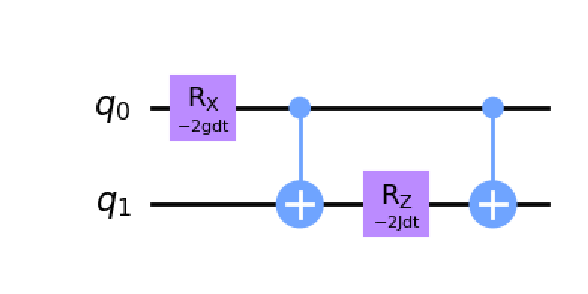
\includegraphics[height=5cm]{quantum_circuit.eps}
    \caption{1ステップの計算回路}
    \label{1steps}
\end{figure}
あとは粒子数、及び時間分割の回数分この回路を繰り返せば、$t=t_{1}$から$t=t_{2}$までの状態をN分割してその状態を再現することが出来る。
 
\subsection{断熱定理による基底状態の遷移}
前節で時間発展を量子回路上で表したが、この時間発展回路をどのように生かすべきであろうか？本節では、この時間発展を活かした最たるアルゴリズムとして、「断熱準備」を導入し、実際に物理量を計算する。\\
\\
まず、断熱準備を述べる際に、キーワードとなる定理として、「断熱定理」が挙げられる。そのstatementは以下である。
\begin{theorembox}{断熱定理}
以下のようなハミルトニアン系を考える。ただし、摂動を加える時間tをt=[0,T]とする。
\begin{equation}\begin{split}
    H(t) = (1 - \frac{t}{T}) H_{0} + \frac{t}{T}H_{1}
\end{split} \end{equation}
この時、エネルギースペクトラムが離散的であり、エネルギーの差に比べてTが十分に大きいなら、離散間の準位を変えることなく状態が遷移する。
\end{theorembox}
この定理を用いると、例えば相互作用系による非自明な基底状態が、自由な系の自明な基底状態からの時間発展により得ることができる。この非自明な基底状態の用意の方法を、「断熱準備」という。\\
\\
以下、この断熱準備を横磁場イジングモデルに適用することを考える。仮に$J=0$であればその基底状態は自明であるが、$J\neq 0$ならば基底状態を考察することは一般に難しい。しかし断熱原理の計算を応用することによりバンド間に十分差が存在するなら基底状態を時間発展により生成できる。断熱定理を適用するために必要な議論を考える。初期状態として横磁場のみ、摂動として相互作用の効果を加えることを考えると、全体のハミルトニアンは以下のように記述される。
\begin{equation}\begin{split}
    \hat{H}(s)=-sJ\sum_{n=0}^{N-1}\hat{\sigma}_{i+1}^{Z} \hat{\sigma}_{i}^{Z} -Jg\sum_{n=0}^{n-1} \hat{\sigma}_{i}^{Z}
\end{split} \end{equation}
イジングモデルにおいてエネルギー固有値の大きさを議論する。Jordan-wigner変換による議論より、以下のstatementが成立する。
\begin{resultbox}{横磁場イジングモデルとFree-fermion系の双対性}
横磁場イジングモデルのハミルトニアンは、以下のハミルトニアンを持つFree-fermionの系として書き換えられる。
\begin{equation}\begin{split}
    \hat{H} = \sum_{k} \epsilon_{k}(\gamma^{\dagger}_{k} \gamma_{k}-\frac{1}{2})
\end{split} \end{equation}
ただし、$\gamma^{\dagger}_{k}, \gamma_{k}$はフェルミオンの生成消滅演算子である。
\end{resultbox}
断熱定理の議論により、あらゆるバンド間に対して遷移確率が小さくなるのはポテンシャルが断熱的に加わる時間Tが以下の式を満たす場合となる。
\begin{equation}\begin{split}
    T >> \frac{max(\bra{\psi_{0}^{m}}\pdv{\hat{H}}{s}\ket{\psi_{0}^{n}})}{|min(E_{n}-E_{m})|^{2}}
\end{split} \end{equation}
以上の議論を踏まえ、横磁場イジングモデルの真空の性質を考察する。
まず、基底状態が生成されているかのある種のテストを考察する。断熱定理により基底状態が構成できているとすると、断熱的に摂動を取り除くと自明な基底状態に戻る。従って摂動を取り除いた後の状態のうちの基底状態以外の割合を計測する。計算に使用するN=5及びN=15の場合、結果は図\ref{vacuum_test_5}、及び図\ref{vacuum_test_15}となる。
\begin{figure}[h]
    \centering
    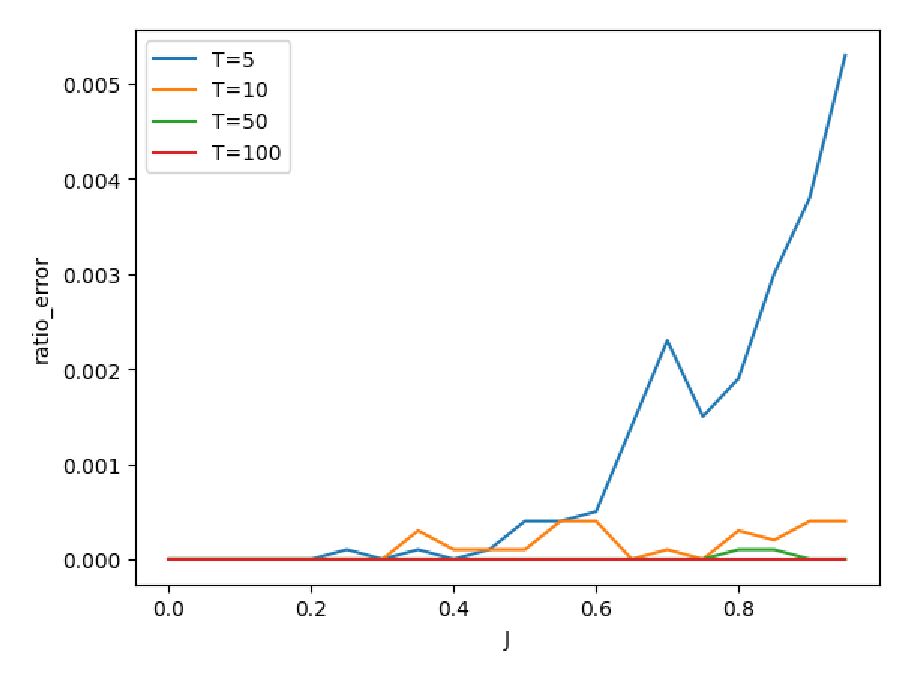
\includegraphics[height=5cm]{T_dependence_of_missing.eps}
    \caption{摂動排除後の基底状態以外の確率分布(N=5)}
    \label{vacuum_test_5}
\end{figure}
\begin{figure}[h]
    \centering
    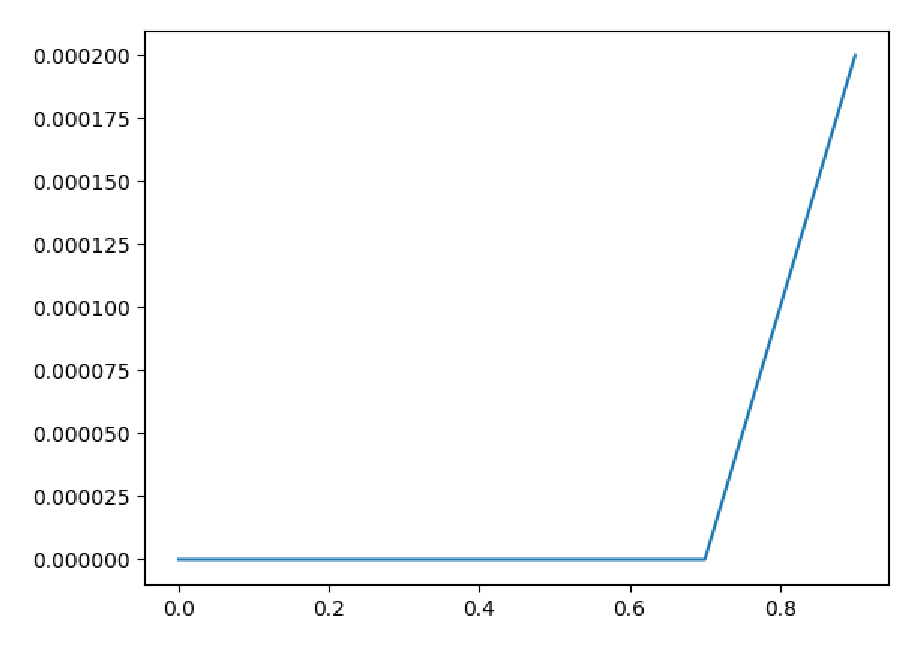
\includegraphics[height=5cm]{vacuum_estimation.eps}
    \caption{摂動排除後の基底状態以外の確率分布(N=15)}
    \label{vacuum_test_15}
\end{figure}
N=5においてはTが大きい場合高い確率で基底状態が取り出せていると言える。また、N=15における基底状態はJ=0.7程度からそれ以外の状態が混ざり始めるといえる。\\
次にN=15におけるx方向の磁化$<\sigma_{x}>$の計算結果は図\ref{ising_zika}のようになる。\\
\begin{figure}[h]
    \centering
    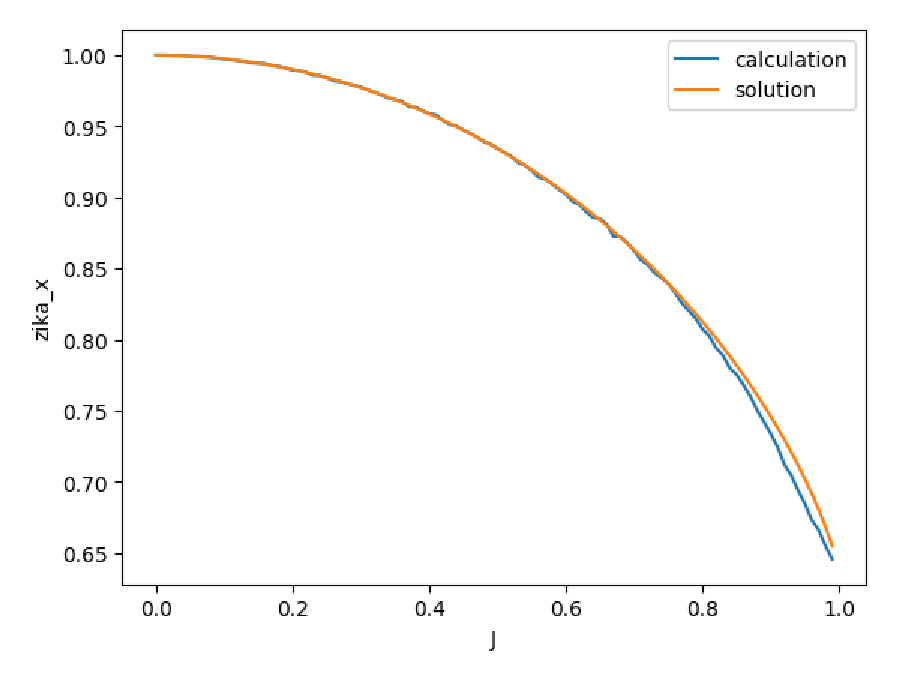
\includegraphics[height=5cm]{magnetization.eps}
    \caption{磁化$<\sigma_{x}>$のJ依存性}
    \label{ising_zika}
\end{figure}
厳密解は以下のように与えられる。ただし、これは文献から引っ張ってきた。
\begin{equation}\begin{split}
    <\sigma_{x}>=\frac{1}{\pi}\int_{0}^{\pi} dk\frac{1+\frac{J}{g}cosk}{\sqrt{1+(\frac{J}{g})^{2}+2\frac{J}{g}cosk}}
\end{split} \end{equation}
シミュレータと厳密解と比較すると、Jが小さい領域においては一致することが分かる。Jが大きい領域においては厳密解とのずれがみられるが、その理由はエネルギー準位の狭まりによる基底状態からの遷移によると考えられる。根拠としてテストにおける基底状態以外の発生点と磁化がずれ始める点が一致しているためである。\\
\\
次に位相推定アルゴリズムを用いて基底状態のエネルギーを計算する(N=5)。その結果は図\ref{ising_energy}となる。
\begin{figure}[h]
    \centering    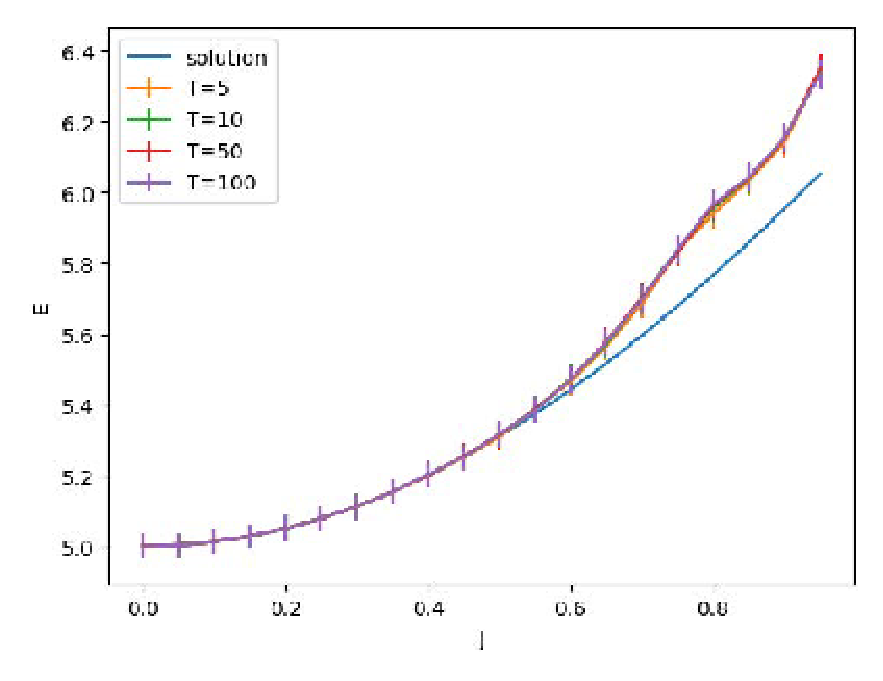
\includegraphics[height=5cm]{J_dependence_of_energy.eps}
    \caption{エネルギーのJ依存性}
    \label{ising_energy}
\end{figure}
ただし、エネルギーの厳密解は以下の通りである。
\begin{resultbox}{横磁場イジングモデルの基底エネルギー}
\begin{equation}\begin{split}
    E_{0}=-J\sum_{k}(1+g^{2}-2gcos(\frac{2\pi k}{N}))^{\frac{1}{2}}
\end{split} \end{equation}
\end{resultbox}
注目すべき点として、基底状態のテストで問題が生じない場合でもJが小さい領域から厳密解とエネルギーがずれている点である。まずこれを準位の遷移によるものだと考えた場合、T依存性が存在するはずである。しかしグラフによると分岐地点にT依存性が存在しないように見える。その他位相推定の時間分割幅など変数を変えて計算してきたが、いずれの場合も有意な依存性は見られなかった。私見では相互作用Jが1に近づくにつれエネルギー準位間が狭まるので、そのことが位相推定アルゴリズムにおいて悪影響を及ぼしているのではないかと考えている。\\
(完全に後日談だが、Chatgptに聞くと、普通に第１励起に言ってる可能性が高いらしい。磁化は第１と励起の間で差が出にくいため、磁化では問題ないらしい。定性的にも完全にそうっぽい？)

\subsection{量子計算によるRenyiエントロピーの計算}
昨今、量子論の解析においてエンタングルメントエントロピーといった物理量が重要な役割を果たしている。例えばエンタングルメントエントロピーは、相転移の秩序変数となりうる。場の理論などにおいては一般的にエントロピーを計算することが難しいが、量子計算の手法を用いた場合、特に2次のrenyiエントロピーについては簡単なアルゴリズムで計算できることが知られている。これは系の分解において量子もつれの有無を発見することが出来る。\\
\\
Hilbert空間の次元がそれぞれ$N_{A},N_{B}$となる複合系ABが存在したとして、その状態$\ket{\psi}_{AB}$を以下のように展開する。
\begin{equation}\begin{split}
    \ket{\psi}_{AB}=\sum_{i,j}c_{i,j}\ket{i_{1}\cdots i_{N_{A}},j_{1}\cdots j_{N_{B}}}
\end{split} \end{equation}
仮に同じHilbert空間を持つ2つの状態が存在したとして、そのSWAPゲートを以下のように定義したとする。
\begin{defbox}{SWAPゲート}
\begin{equation}\begin{split}
    &SWAP_{A}(\ket{\psi}_{AB}\ket{\psi'}_{AB})\\
    &=SWAP_{A}(\sum_{i,j}\sum_{i',j'}c_{i,j}c'_{i',j'}\ket{i_{1}\cdots i_{N_{A}},j_{1}\cdots j_{N_{B}}}\ket{i'_{1}\cdots i'_{N_{A}},j'_{1}\cdots j'_{N_{B}}})\\
    &=\sum_{i,j}\sum_{i',j'}c_{i,j}c'_{i',j'}\ket{i'_{1}\cdots i'_{N_{A}},j_{1}\cdots j_{N_{B}}}\ket{i_{1}\cdots i_{N_{A}},j'_{1}\cdots j'_{N_{B}}})
\end{split} \end{equation}
\end{defbox}
実は、このSWAPゲートの期待値は、２次renyiエントロピーそのものである。
\begin{resultbox}{SWAPゲートの期待値}
\begin{equation}\begin{split}
    tr_{A}(\rho^{A})^{2}=\bra{\psi}\bra{\psi}SWAP_{A}\ket{\psi}\ket{\psi}
\end{split} \end{equation}
\end{resultbox}
\begin{proofbox}
まず密度行列$\rho^{A}$の(i,i'')成分は$\bra{i}\rho^{A}\ket{i'}=\sum_{j}\bra{j}\bra{i}\rho\ket{i'}\ket{j}=\sum_{j}c_{i',j}^{*}c_{i,j}$である。左辺に関しては以下のように変形できる。
\begin{equation}\begin{split}
      &(\bra{\psi}_{AB}\bra{\psi}_{AB})SWAP_{A}(\ket{\psi}_{AB}\ket{\psi}_{AB})\\
      &=\sum_{m,n}\sum_{m',n'}c_{m,n}^{*}c_{m',n'}^{*}\bra{n_{1}\cdots n_{N_{A}},m_{1}\cdots m_{N_{B}}}\bra{m'_{1}\cdots m'_{N_{A}},n'_{1}\cdots n'_{N_{B}}}\\
      &\sum_{i,j}\sum_{i',j'}c_{i,j}c_{i',j'}\ket{i'_{1}\cdots i'_{N_{A}},j_{1}\cdots j_{N_{B}}}\ket{i_{1}\cdots i_{N_{A}},j'_{1}\cdots j'_{N_{B}}})\\   		  &=\sum_{m,n}\sum_{m',n'}\sum_{i,j}\sum_{i',j'}c_{m,n}^{*}c_{m',n'}^{*}c_{i,j}c_{i',j'}\delta_{n,i'}\delta_{m,j}\delta_{n',i}\delta_{m',j'}\\
      &=\sum_{i,j}\sum_{i',j'}c_{i',j}^{*}c_{i,j'}^{*}c_{i,j}c_{i',j'}\\
      &=\sum_{i,i'}\rho^{A}_{i,i'}\rho^{A}_{i',i}\\
	&=tr_{A}(\rho^{A})^{2}
\end{split} \end{equation}
最後の式は２次renyiエントロピーそのものである。従って、2次のrenyiエントロピーはSWAPゲートを挟んだ内積により計算される。
\end{proofbox}
上記を用いて、2次renyiエントロピーが量子コンピュータ上で計算できることを示す。
2準位系においてSWAPゲートはCNOTゲート3回により実装されるため、比較的自明に実装が出来るユニタリーゲートである。問題はこのSWAPゲートの期待値をどのように計算するかであるが、オペレータの期待値は「アダマールテスト」により計算されることは、前節で見た通りである。\\故にアダマールテスト
を用いて、例えばBell状態における2次のRenyiエントロピーを計算できる。Bell状態の2次renyiエントロピーは以下のように計算される。
\begin{equation}\begin{split}
    tr_{B}(\ket{Bell}\bra{Bell})&=(\bra{0}\frac{(\ket{00}+\ket{11})(\bra{00}+\bra{11})}{2}\ket{0}+\bra{1}\frac{(\ket{00}+\ket{11})(\bra{00}+\bra{11})}{2}\ket{1}\\
    &=\frac{1}{2}(\ket{0}\bra{0}+\ket{1}\bra{1})
\end{split} \end{equation}
    \begin{equation}\begin{split}
        f_{2}(\ket{Bell}\bra{Bell})=-log(tr_{A}(\frac{1}{2}(\ket{0}\bra{0}+\ket{1}\bra{1}))^2)
        =-log(-\frac{1}{2})=1
    \end{split} \end{equation}
アダマールテストにより実装した回路で計算したものと比較した。結果が図\ref{Bell_renyi}である。(ただし、renyiエントロピーを計算する際に求めたshot数は20000,試行回数は10000として試行回数に対して平均、及び標準誤差を計算した)。
\begin{figure}[h]
    \centering
    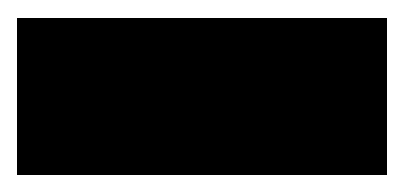
\includegraphics{renyi_entropy_of_bell.eps}
    \caption{Bell状態の２次renyiエントロピーの厳密解と計算結果}
    \label{Bell_renyi}
\end{figure}
確かに、誤差の範囲内でBell状態の2次renyiエントロピーが計算できたと言える。\\
先ほど求めた横地場イジングモデルの基底状態に対して2次renyiエントロピーのアルゴリズムを適用する。まず粒子数N、スピン鎖を分割した際の分割空間内の粒子数Lとした際、$N,L \to \infty$の場合の２次renyiエントロピーの厳密解は以下の通り。
\begin{equation}\begin{split}
    f_{2}(\rho)&=-\frac{1}{6}ln(k^{2}k'^{\frac{3}{2}}\frac{(1+k')^{2}}{1-k'}) +\frac{1}{2}ln2\\
    k&=\frac{J}{g} \:\:\:\:\:\:k'=\sqrt{1-k^{2}}
\end{split} \end{equation}
厳密解及びアルゴリズムより求められた2次renyiエントロピーは図\ref{ising_renyi}(ただしN=10,L=5)。
\begin{figure}[h]
    \centering
    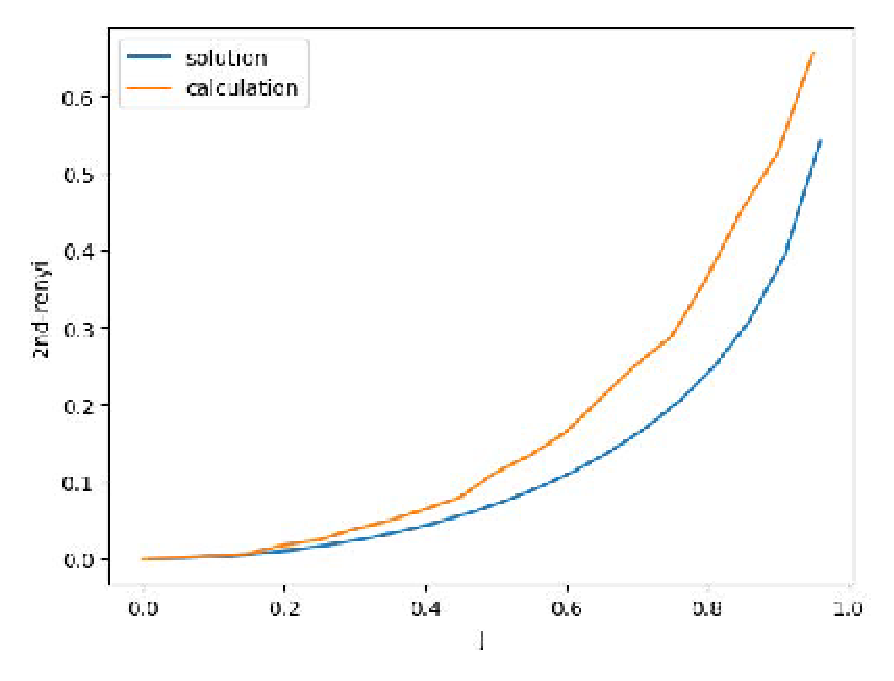
\includegraphics[height=5cm]{renyi_of_Ising.eps}
    \caption{イジングモデル基底状態の2次renyiエントロピー}
    \label{ising_renyi}
\end{figure}
まず摂動論的に考えた場合、J<<gの項では$\ket{00\cdots 0}$の項の係数が1に近い値となるため$f_{2}(\rho)<<1$となる。従って摂動論的には正しい計算結果を得られたといえる。しかし、Jが大きくなると量子計算で出した数値と厳密解にずれが生じる。このことは粒子数が影響していると考えられる。2次renyiエントロピーの大まかなJ依存性としては似た傾向が存在していると考えられる。

\subsection{断熱量子計算による最適化問題の解探査}
実は今行った量子シミュレーションの考え方は、単なる物理の問題を解く以上の意味がある。というのも、実は数学的には、いくつかの物理系の基底エネルギーを求める問題が、最適化問題の解を探すことと等価となることが知られているためである。ここでは、具体的な問題を通し、このstatementを確認する。

\subsubsection{最適化問題について}
例えばセールスマンが候補となるいくつかの会社に対し、営業をかけねばならないとする。このセールスマンは少しでも楽をするため、最も移動距離が短い配達経路を探そうとするだろう。ではこの時、そのような経路はどのように見つけるだろうか？\\
「最適化問題」とは、このように決められた条件の中、コスト関数\footnote{先ほどのセールスマンの例の場合、コスト関数は移動距離である。}が最小になるような組み合わせを見つける問題のことである。上記の例は、「巡回セールスマン問題」と呼ばれる最適化問題の有名な例である。\\
\\
最適化問題の解を調べることは、（少なくとも知られている限りでは）古典コンピュータの範囲では、計算量の観点から非常に難しい。先ほどのセールスマンの例では、どの経路が最適化を調べるためには、全ての経路について考えて、そこから最短経路を求めねばならない。地点の数がN個あるとすると、すべての経路を考えるのはN地点の並び替え問題と等価であるため、その計算コストは、
\begin{align*}
    N!>>2^{N}
\end{align*}
故に、最適化問題を解くためには、巡回セールスマンの例では、地点が増えるごとに起きる、指数よりさらに酷い計算量爆発を乗り越えねばならない。\\
\subsubsection{maxcut問題}
量子計算を用いることは、この最適化問題を解くための有力な候補である。このことを、簡単な例であるmax-cut問題を例として見てみる。まずmax-cut問題とは、以下のような問題である。
\begin{defbox}{max-cut問題}
    頂点とそれをつなぐ辺からなるグラフが与えられたとする。max-cut問題とは、それらの頂点を２つのグループに分けた際、そのグループの境界となる辺の数が最大となるようにグループを分ける問題である\footnote{max-cutという名前の由来は、点をグループ分けする行為が、境界とする辺を切断する行為に等しいことである。上図では、右図に走る紫の線が切り取り線に対応}。
    \begin{center}
  \includegraphics[width=0.8\linewidth]{Max-cut.eps}
  \captionof{figure}{max-cut問題の模式図。左図が与えられたグラフで、右図が紫と白に頂点をグループ分けした図\\
  (引用：Quantum approximate optimization algorithm)}
  \label{fig:maxcut}
\end{center}
\end{defbox}
max-cut問題は、以下のような問題にすげ替えることができる。
\begin{resultbox}{maxcut問題の解法}
    各頂点のグループ分けを、$x^{i}\in\{0,1\}$で表す。このとき、max-cut問題の解を探すことは、以下を求めることに等しい。
    \begin{align*}
        max_{x\in\{0,1\}^{n}}\, \sum_{(i,j)}x^{i}+x^{j}-2x^{i}x^{j}
    \end{align*}
    ただし、総和の下の(i,j)は、グラフ内での隣接点全ての組に対する足し算である。
\end{resultbox}
\begin{proofbox}
    点をグループ分けした際に、ある２点の間の辺が境界になるか否かを特徴付けられれば、あとはその足し合わせで境界となる辺の数が求まる。\\
    故に、確認すべきは、足し合わせの中の式が、本当に「境界か否かを特徴づけるコスト関数であるか」である。max-cutの際のコスト関数は、問題の定義より、以下のとおりである。
    \begin{align*}
        f(x_{i},x_{j})=
        \begin{cases}
        1\quad(\text{$x_{i}$と$x_{j}$の値が異なる})\\
        0\quad(\text{$x_{i}$と$x_{j}$の値が等しい})
        \end{cases}
    \end{align*}
    $x_{i},x_{j}$に(0,1)を代入していくと、$x^{i}+x^{j}-2x^{i}x^{j}$は確かにこれを満たすことがわかる。\\
    \\
    max-cut問題の解は、境界となる辺の最大値であるため、確かに(題意)の値がそのままMax-cut問題の解となる。
\end{proofbox}
max-cut問題の解を与えるためには、すべての点での{0,1}を総当たりで調べていく必要があるため、n頂点グラフでのmax-cut問題の計算コストは$O(2^{n})$である。故に、古典計算の範疇では、確かにこの問題を解くのは難しい。\\
\\
反面、このMax-cut問題は、量子計算を用いることで、より少ない計算量で解ける事が知られている。セットアップは以下のとおりである。
\begin{setupbox}{Max-cut問題の量子計算での解法}
\begin{enumerate}
    \item スピンによる変数の置き換え\\
    グラフ頂点にスピンを置き、グループ分けをスピンの上下で表現する。この際、$x_{i}$の値は、以下のような行列の固有値に置き換えられる。
    \begin{align*}
        x_{i}\to \frac{1+Z_{i}}{2}
    \end{align*}
    \item コスト関数をハミルトニアンに置き換える。\\
    \begin{align*}
        &\sum_{(i,j)}x^{i}+x^{j}-2x^{i}x^{j} 
        \\\to H_{cost}\equiv&- \sum_{(i,j)}\frac{1+Z_{i}}{2}+\frac{1+Z_{j}}{2}-\frac{(1+Z_{i})(1+Z_{j})}{2}\\
        =& \sum_{(i,j)}\frac{-1+Z_{i}Z_{j}}{2}
    \end{align*}
    この時、定義より、max-cut問題の解は、このハミルトニアンの基底エネルギーの-1倍に等しい。
    \item 基底状態準備によるmax-cut問題の解の推定\\
    量子計算ではハミルトニアンを与えた際に基底状態や基底エネルギーを求める方法が知られているので、それを用いてmax-cut問題の解を推定。
\end{enumerate}
\end{setupbox}
量子計算では、上記のセットアップを用いることで、max-cut問題を解ける。\\
\\
以下では、簡単な演習として、実際にグラフを与えて、それのmax-cut問題を解くことにする。簡単な例として、正方形のグラフのmax-cut問題を考える。グラフは、下図の左側で与えられる。
\begin{center}
  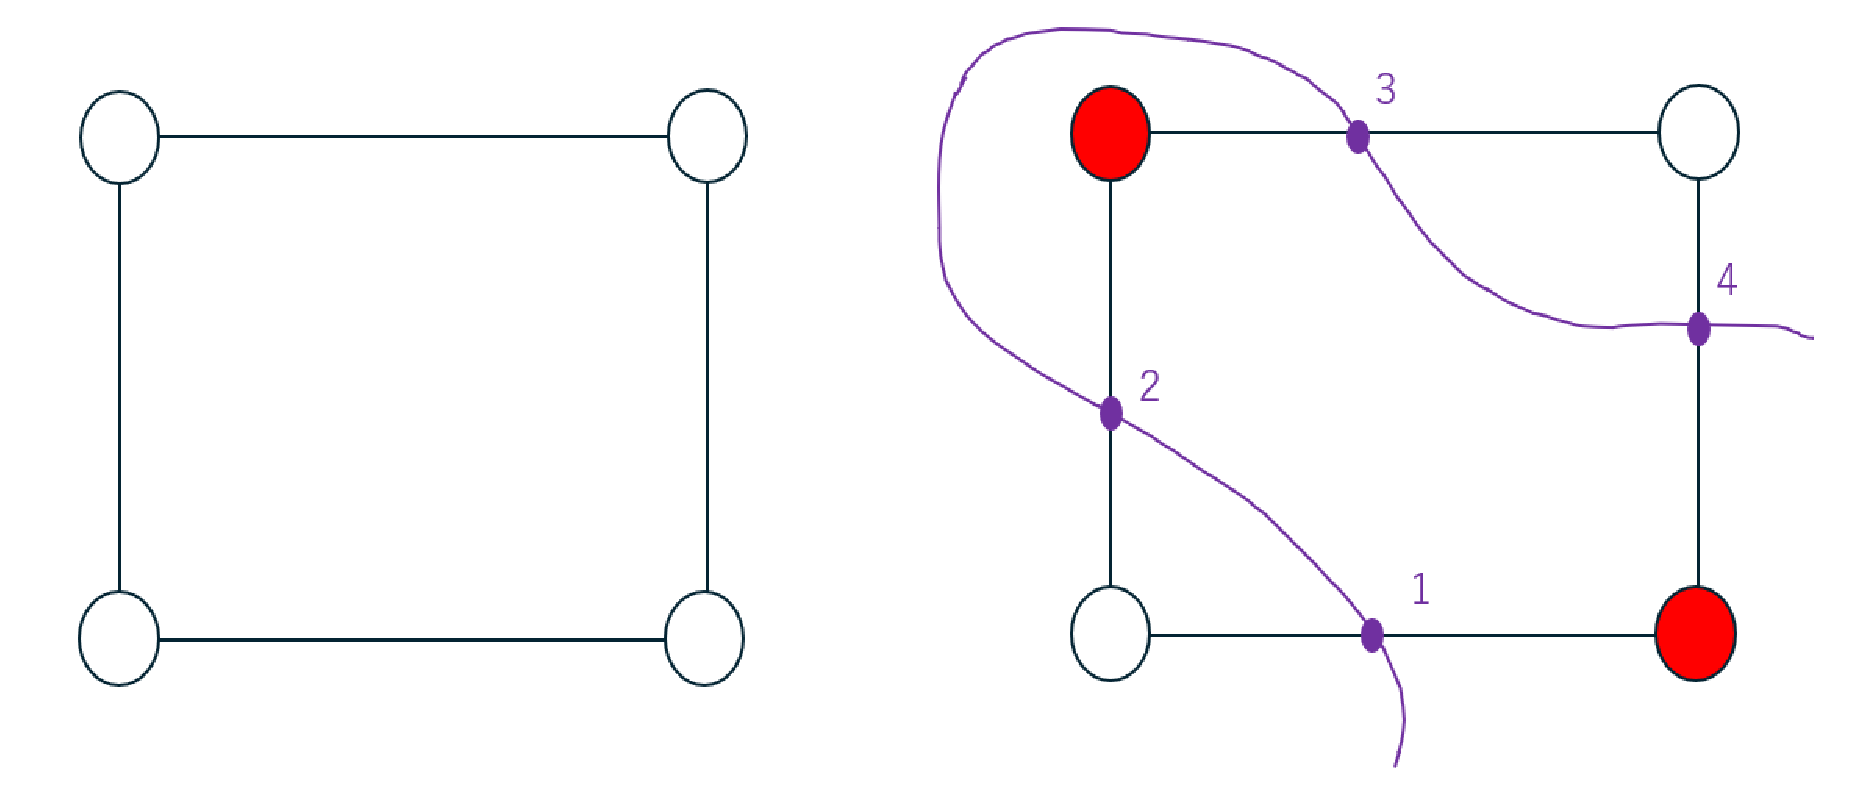
\includegraphics[width=0.8\linewidth]{setup_maxcut.eps}
  \captionof{figure}{正方形のグラフ（左側）、およびそのmax-cut(右側)}
  \label{fig:setup_maxcut}
\end{center}
上図の右側から、明らかに対角となる頂点同士を分けたものがmax-cut問題の解となる。故に、
\begin{align*}
    \text{(正方形max-cut問題の解)}=4
\end{align*}
以下では、断熱量子計算のセットアップのもと、この解が再現できるか確かめる。ハミルトニアンのセットアップとして、例えば以下を採用する。
\begin{align*}
    H(t)=(1-\frac{t}{T})\sum_{i}X_{i}+\frac{t}{T}\sum_{i}\frac{-1+Z_{i}Z_{i+1}}{2}
\end{align*}
あとはこれの時間発展を行い、終状態でのエネルギーを計算してやれば良い。この場合、やるべきシミュレーションは先ほど導入したイジング模型の$(J,g)=(\frac{1}{2},g)$における時間発展である。\\
\\
結果としては、以下のようになる(計算はQiskitで行った。詳細なプログラミングは付録で与えているので、確認して欲しい。)。
\begin{resultbox}{計算結果}
    \begin{align*}
    \text{(理論値)}&=4\\
    \text{(実験値)}&=3.9884\\
    \text{(誤差)}&=| \text{(理論値)}-\text{(実験値)}|=0.0116
\end{align*}
\end{resultbox}
確かに、小数第1位までの精度で正しい結果を与えている。

\section{量子特異値変換}
ここまで、量子優位性が期待されている代表的なアルゴリズムとして、「位相推定」、「Groverのアルゴリズム」、「ハミルトニアンシミュレーション」を見てきた。無論、これら以外にも、多数の量子アルゴリズムが提案されている。\\
\\
しかし、これらのアルゴリズムは、それぞれ個別に考案されたものであり、その構成原理が必ずしも明確に統一されているわけではない。新たな量子アルゴリズムを「より効率的に」設計する際には、「そもそも量子計算で何ができるか？」ということを知ることが求められる。この視点から、量子アルゴリズムをより構成論的・統一的に構築する視点が求められる。\\
そこで本章では、多くの量子アルゴリズムを包括的に理解できる枠組みである、量子特異値変換（Quantum Singular Value Transformation; QSVT）について解説する。QSVTを理解することで、既存の量子アルゴリズムを統一的な観点から捉えられるだけでなく、新たな量子アルゴリズムを設計するための基本的な指針を得ることができる。\\
\\
なお、最初に述べておくが、この章にも直感的な描像は、導入を除いて存在しない。故に、「なぜ書いた人はこれを思いついたのか？」という理由を探ることは多分無駄である。「原論文の著者は天才だったんだな」と思いつつ見てほしい。

\subsection{アイデア}
量子特異値変換の最大の利点は、多様な量子アルゴリズムを「固有値に対する関数変換」という共通の視点から理解できる点にある。\\

その考え方を理解するために、まずは量子アルゴリズムが本質的にどのような操作を実現しているのかを確認していく。
\begin{setupbox}{ハミルトニアンシミュレーション}
ハミルトニアンシミュレーションとは、以下を行う回路である。
\begin{align*}
    \ket{\psi}\to e^{-iHt}\ket{\psi}
\end{align*}
\end{setupbox}
\begin{setupbox}{Groverのアルゴリズム}
Groverのアルゴリズムとは、以下のreflectionを複数回作用させる回路である。
\begin{align*}
    \Pi=I-\sum_{x}2\ket{x}\bra{x}
\end{align*}
特に、最適化問題などでは、解空間を、ハミルトニアンを基底状態に写像することが多い。この場合、reflectionは以下の通りである。
\begin{align*}
    \Pi= \sum sign(\hat{H}-\mu I)\ket{E}\bra{E}
\end{align*}
\end{setupbox}
これらの例から分かるように、少なくとも本論で今まで扱った量子アルゴリズムは、ハミルトニアンの固有状態を保ったまま、固有値に対して関数変換を施す操作として理解することができる。
\begin{resultbox}{量子回路の共通操作}
\begin{align*}
    \ket{E}\bra{E}\to f(E)\ket{E}\bra{E}
\end{align*}
\end{resultbox}
故に、このような関数群を実装する一般的な方法が存在すれば、それは上記で紹介した量子アルゴリズムを包括する統一的な枠組みとなることが期待される。\\
\\
量子特異値変換（Quantum Singular Value Transformation; QSVT）とは、あるクラスの関数群に対して、特定の手順を踏むことで上記の応答を行う回路を実装する手法である。\\
\\
ただし、一点注意事項が存在する。QSVTは、あくまでハミルトニアンの多項式関数を実装するための方法論にすぎないので、それ以外の、量子の別側面に着目するアルゴリズムとの関係は確約されてない。位相推定は、固有値に応じた変換を状態へ施すのではなく、固有位相を補助レジスタへ読み出すことを目的とする。この意味で、通常の位相推定はQSVTが直接統一するアルゴリズムとは関係がないとまでは言わないが、ある種目的が異なる。

\subsubsection{Block-encoding}
以下では、その具体的な実装手順について順に見ていく。\\
\\
ここでは、多項式近似の実装の共通言語となる、「Block-encoding」について定義する。
\begin{defbox}{Block-encoding}
Block-encodingとは、ある行列Aを、以下のように、Ancillaを加えたユニタリ回路Uの一部に埋め込むことである\footnote{ただし、ユニタリ行列に埋め込むための条件として、色々な条件が存在する。例えば$|H|\leq 1$。後でこの条件を証明するが、今は仮定として暗に置く。}。
\begin{align*}
    U=\begin{pmatrix}
        H & \cdot \\
        \cdot & \cdot
    \end{pmatrix}
\end{align*}
もしくは、同等の表現方法として、Ancilla\footnote{以下では、Block-encoding由来のAncillaを$\ket{}_{a}$と記述する。ブラベクトルは省略}を用いた以下の表現方法が挙げられる。
\begin{align*}
    H=\bra{0}U\ket{0}_{a}
\end{align*}
\end{defbox}
この行列Hが、例えばハミルトニアンシミュレーションの場合、ハミルトニアンに相当する。\footnote{ハミルトニアンはあくまでエルミートな行列なので、こんなユニタリの中に埋め込むのは無理やんけと思われるかもしれないが、結果としては、規格化さえすれば大丈夫である。詳しくはハミルトニアンシミュレーションの項で見る。}\\
このBlock-encodingを用いた手法を考えることで、ユニタリであるという制約に縛られることなく、より広いクラスの関数を実装できる。\\
\\
問題は、Block-encodingの形で行列Aが与えられた際に、どのようにしてその多項式を位相として吐き出す回路を実装できるかである。単純な例から話を進める。例えば、まずは多項式実装の一番目に簡単な例として、以下のような回路の実装方法を考える。
\begin{problembox}{Aを作用させる回路}
AのBlock-encoding回路Uが与えられたとして、以下のような回路は実装可能？
\begin{align*}
    \ket{\psi}\bra{\psi}\to H\ket{\psi}\bra{\psi}
\end{align*}
\end{problembox}
これは、以下の手続きにより簡単に実装可能。
\begin{setupbox}{回路の実装}
\begin{enumerate}
    \item 初期状態を用意(ただし、２つ目のketはancillaを表す)
    \begin{align*}
        \ket{\psi}\ket{0}_{a}
    \end{align*}
    \item ユニタリ行列Uを作用
    \begin{align*}
        U\ket{\psi}\ket{0}_{a}=H\ket{\psi}\ket{0}_{a}+\sqrt{1-||H\ket{\psi}||^{2}}\ket{\psi^{\perp}}
    \end{align*}
    \item Ancillaのみを観測して、結果が0であるものをpost-selection
    \begin{align*}
        \ket{f}=\bra{0}U\ket{0}_{a}\ket{\psi}=H\ket{\psi}
    \end{align*}
\end{enumerate}
\end{setupbox}
これは自明すぎてあまり面白くない。問題は、次のような、二番目に単純な回路の構築方法である。
\begin{problembox}{$H^{2}$を作用させる回路}
    HのBlock-encoding回路Uが与えられたとして、以下のような回路は実装可能？
\begin{align*}
    \ket{\psi}\bra{\psi}\to H^{2}\ket{\psi}\bra{\psi}
\end{align*}
\end{problembox}
これを行うためにナイーブに思いつく方法としては、Uを2回かけることが挙げられる。この場合どうなるかを見てみて、何が実装の際に問題なのかを把握する。
\\
ただし、以下より簡単のため、初期状態としてHの固有状態$\ket{\lambda}$を作用させるケースを考える。
\begin{setupbox}{Uを2回作用させる回路}
    \begin{enumerate}
        \item 一回目のUの作用\\
        \begin{align*}
            U\ket{\lambda}\ket{0}_{a}=H\ket{\lambda}\ket{0}_{a}+\sqrt{1-\lambda^{2}}\ket{\lambda^{\perp}}
        \end{align*}
        \item 二回目のUの作用\\
        ここでは、一回目の作用で出てきた項それぞれへの作用を考える。
        \begin{align*}
           U (H\ket{\lambda}\ket{0}_{a})=H^{2}\ket{\lambda}\ket{0}_{a}+\sqrt{1-|\lambda|^{2}}\ket{\lambda^{\perp}}
        \end{align*}
        第２項目は以下の通りである。
        \begin{align*}
            U\ket{\lambda^{\perp}}=\sum_{\lambda'}a_{\lambda}^{\lambda'}\ket{\lambda'}\ket{0}_{a}+b\ket{\lambda'^{\perp}}
        \end{align*}
        \item ポストセレクション\\
        ancillaで0を観測した状態を終状態とすると、以下のようになる。
        \begin{align*}
            \ket{f}=H^{2}\ket{\lambda}\ket{0}_{a}+\sum_{\lambda'}a_{\lambda}^{\lambda'}\ket{\lambda'}\ket{0}_{a}
        \end{align*}
    \end{enumerate}
\end{setupbox}
２回目のUを当てた際、一般的には直交補空間から戻り項が出現し、その結果「余分な因子」が出現するため、上記のナイーブな適用では目的の回路を構成できない。\\
\\
結論からの逆算になってしまうが、上記で出てきた問題の種類として、避けなければならない問題と避けなくても良い問題の2種類が存在する。
\begin{enumerate}
    \item 避けなければならない問題\\
    ポストセレクション後の状態として、問題なのが「あらゆる固有値の足し合わせ」となっている点である。この部分は直交補空間、つまりBlock-encodingの未知の部分に依存する項となる為、この項が存在してしまうと問題がケースバイケースとなって制御不能となる。この為、Uでエネルギー固有空間がleakする問題は、絶対に避けなければならない。
    \item 避けなくても良い問題\\
    逆に避けなくても良いのはUを2回かけても答えが$H^{2}$にならない問題そのものである。極論、求めたい関数近似は冪乗の形で書けるものでなくても良いため、あーアプローチが悪かったなー別のがいいかもなーくらいの感覚でいい。
\end{enumerate}
少なくとも、Block-encodingからダイレクトで与えられたUは、上記の2乗の計算から「避けなければならない問題」を含んでいる。この問題を回避するために、Block-encoding回路Uを「改造」しなければならない。この改造した回路のことを、原論文に習い「iterate W」と呼ぶことにする。以下では、iterateの上手い構成方法、「Qubitization」を与える。

\subsubsection{iterate Wの構成(Qubitization)}
まずは、iterate Wを構築する際にほしい性質を述べる。これは上記の解析、および問題提起から、以下のような性質が挙げられる。
\begin{enumerate}
    \item WはHのBlock encodingである。
    \item WはHilbert空間$H_{\lambda}=<\ket{\lambda}\ket{0}_{a},W\ket{\lambda}\ket{0}_{a}>$の下で閉じている。
\end{enumerate}
これを満たすようなiterate Wとして、例えば以下が与えられる。
\begin{resultbox}{iterate Wの具体的な形}
    \begin{align*}
        \hat{W}\equiv \bigoplus_{\lambda} \begin{pmatrix}
            \lambda & -\sqrt{1-\lambda^{2}}\\
            \sqrt{1-\lambda^{2}} & \lambda
        \end{pmatrix} =exp(-iYarccos(\lambda))
    \end{align*}
    ただし、この２次元行列は、以下のHilbert空間上に与えられる。
    \begin{align*}
        H_{\lambda}=<\ket{\lambda}\ket{0}_{a},\ket{\lambda^{\perp}}>
    \end{align*}
\end{resultbox}
上記のiterate Wが上記の性質を満たすことを見る。
\begin{proofbox}
\begin{enumerate}
    \item Block-encodingについて
    \begin{align*}
        \bra{\lambda}\bra{0}W\ket{\lambda}\ket{0}_{a}=\lambda
    \end{align*}
    全ての$\ket{\lambda}$に対して上記が成立するため、
    \begin{align*}
        \bra{0}W\ket{0}_{a}=\lambda\ket{\lambda}\bra{\lambda}=H
    \end{align*}
    \item 閉じているか否か
    \begin{align*}
        W^{2}&=\bigoplus_{\lambda} \begin{pmatrix}
            2\lambda^{2}-1 & -2\lambda\sqrt{1-\lambda^{2}}\\
            2\lambda\sqrt{1-\lambda^{2}} & 2\lambda^{2}-1
        \end{pmatrix} \\
        &=\bigoplus_{\lambda} 2\lambda\begin{pmatrix}
            \lambda & -\sqrt{1-\lambda^{2}}\\
            \sqrt{1-\lambda^{2}} & \lambda
        \end{pmatrix}
        -I
    \end{align*}
    故に、以下が成立。
    \begin{align*}
    W^{2}\ket{\lambda}\ket{0}_{a}=2\lambda(W\ket{\lambda}\ket{0}_{a})-\ket{\lambda}\ket{0}_{a}\in <\ket{\lambda}\ket{0}_{a},W\ket{\lambda}\ket{0}_{a}>
    \end{align*}
\end{enumerate}
\end{proofbox}
また、仮にWを掛けた際の直交成分が以下のように記述できたとする。ここはAncilla数依存だったり他のスペクトルが混ざったりするため、こう書ける保証はないが、今後は、簡単のために、このように書けると仮定する（書けない場合は単に表記を変更するだけでいい）。
\begin{align*}
    \ket{\lambda^{\perp}}=\ket{\lambda}\ket{1}_{a}
\end{align*}
この時、iterate Wは以下のように記述可能。
\begin{resultbox}{iterate Wの別記法}
    \begin{align*}
        \bra{0}W\ket{0}_{a}&=H\\
        \bra{1}W\ket{0}_{a}&=-\sqrt{1-H^{2}}\\
        \bra{0}W\ket{1}_{a}&=\sqrt{1-H^{2}}\\
        \bra{1}W\ket{1}_{a}&=H
    \end{align*}
\end{resultbox}
一般には、上記のようなiterateを構成するためには、固有値$\lambda$を知る必要があるため、位相推定のようなアルゴリズムが必要なので難しいと思われるかもしれない。しかし、実はその問題を回避しつつ具体的な回路を構成することが可能であることが示された。この手法のことを、「Qubitization」と呼ぶ。\\
\\
Qubitizationに関する一般的な主張として、以下のようなstatementが成立する。
\begin{theorembox}{Qubitizationの成立条件}
Assumption:
    \begin{enumerate}
        \item HのBlock-encoding回路Uが存在
        \item controll-U及びその逆行列が存在
        \item Ancillaが追加で1つ存在
        \item O(log($dim H$))分のQbit
    \end{enumerate}
    Result:\\
    iterate Wが実装可能
\end{theorembox}
この章の残りでは、上記の定理を、以下のセットアップに沿って証明する。
\begin{setupbox}{Qubitization構成チャート}
    \begin{enumerate}
        \item $W=\big((2\ket{0}_{a}\bra{0}-I)_{ancilla}\otimes I\big)S U$とした際のSの条件を考察
        \item 上記の条件を満たさないUに関しても新しくAncillaを追加することで、1で導いた条件を満たすBlock-encoding行列U'を構成できることを示す。
        \item 構成の際の計算量の確認
        \item $W=SU'$によりiterateを構成可能
    \end{enumerate}
\end{setupbox}
この時、WがiterateであるためのS'の必要十分条件は、以下の通りである。
\begin{resultbox}{iterate構成の必要十分条件}
    \begin{align*}
        \bra{0}SU\ket{0}_{a}&=H\\
        \bra{0}(SU)^{2}\ket{1}_{a}&=I
    \end{align*}
\end{resultbox}
\begin{proofbox}
    iterateの行列表示を再掲する。
    \begin{resultbox}{iterate Wの別記法}
    \begin{align*}
        \bra{0}W\ket{0}_{a}&=H\\
        \bra{1}W\ket{0}_{a}&=-\sqrt{1-H^{2}}\\
        \bra{0}W\ket{1}_{a}&=\sqrt{1-H^{2}}\\
        \bra{1}W\ket{1}_{a}&=H
    \end{align*}
\end{resultbox}
要はWにSの用いた解を代入して上記を満たす条件を探れば良い。\\
    \\
    まずは、iterateの具体系より、少なくとも以下が言える。
    \begin{align*}
        W\ket{\lambda}\ket{0}_{a}=\lambda\ket{\lambda}\ket{0}_{a}+\sqrt{1-\lambda^{2}}\ket{\lambda^{\perp}}
    \end{align*}
    故に、以下も言える。
    \begin{align*}
        \ket{\lambda}\ket{1}_{a}&=\frac{W-\lambda}{\sqrt{1-\lambda^{2}}}\ket{\lambda}\ket{0}_{a}\\
        &=\frac{\big(I\otimes (2\ket{0}_{a}\bra{0}-I)_{ancilla}\big)S U-\lambda}{\sqrt{1-\lambda^{2}}}\ket{\lambda}\ket{0}_{a}\\
        &=\frac{1}{\sqrt{1-\lambda^{2}}}\big((2\bra{0}SU\ket{0}_{a}-\lambda)\ket{\lambda}\ket{0}_{a}-SU\ket{\lambda}\ket{0}_{a}\big)
    \end{align*}
    ここから、特にiterateの内積の上２式を与える必要十分条件が、題意であることを示す。\\
    \begin{enumerate}
        \item $\bra{0}W\ket{0}_{a}=H$の条件\\
        上記で得られたWの作用に$\bra{0}$を作用させると、
        \begin{align*}
            \bra{0}W\ket{0}_{a}\ket{\lambda}=H\ket{\lambda}
        \end{align*}
        全ての$\ket{\lambda}$に対して同様に作用するためには、
        \begin{align*}
            \bra{0}W\ket{0}_{a}=\bra{0}SU\ket{0}_{a}=H
        \end{align*}
        これらは全て同値変形であるため、上記の式は必要十分条件である。\\
        またこの際、得られたSUを改めて代入して、
        \begin{align*}
        \ket{\lambda}\ket{1}_{a}=\frac{1}{\sqrt{1-\lambda^{2}}}\big(\lambda\ket{\lambda}\ket{0}_{a}-SU\ket{\lambda}\ket{0}_{a}\big)
    \end{align*}
        \item $\bra{1}W\ket{0}_{a}=-\sqrt{1-H^{2}}$の条件\\
        上記で得られた$\ket{\lambda}\ket{1}_{a}$の表式にWを作用させると、いろいろ計算して、
        \begin{align*}
            &W\ket{\lambda}\ket{1}_{a}=\frac{\lambda^{2}-\bra{0}(SU)^{2}\ket{1}_{a}}{\sqrt{1-\lambda^{2}}}\ket{\lambda}\ket{0}_{a}\\
            \iff &\bra{0}W\ket{1}_{a}\ket{\lambda}=\frac{\lambda^{2}-\bra{0}(SU)^{2}\ket{1}_{a}}{\sqrt{1-\lambda^{2}}}\ket{\lambda}
        \end{align*}
        これとiterate Wを$\ket{\lambda}$に作用させた際の挙動を比較すると、
        \begin{align*}
            \frac{\lambda^{2}-\bra{0}(SU)^{2}\ket{0}_{a}}{\sqrt{1-\lambda^{2}}}=-\sqrt{1-\lambda^{2}}\iff \bra{0}(SU)^{2}\ket{0}_{a}=1
        \end{align*}
        これらの式も全て同値変形であるため、必要十分条件である。\\
        \\
        あとはこれらを代入すると、残りの関係式も満たせることが確認可能。
        \end{enumerate}
\end{proofbox}
次に、上記を満たすようなiterateの構成を行う。 実は全てのUについて上記を満たすようなSが存在するとは限らない。しかし、Uの方にも多少改造を行った行列U'を作成することで、ありとあらゆるBlock-encoding行列Uに対して上記のようなSを構成することが可能である。\\
以下では、そのような回路S,U'をexplicitに記述する。
\begin{resultbox}{iterate Wの構成(Qubitization)}
まずは、Ancilla1個を追加で加え\footnote{Block-encodingのAncillaとの混同を避けるため、このAncillaを「b」と表記する。元のBlock-encoding由来のAncillaは今まで通り「a」と記述}、以下のような回路を定義する。これは、Uが与えられているといつでも可能である。
\begin{align*}
    U_{CNOT}&\equiv\ket{0}\bra{0}_{b}\otimes I+ \ket{1}\bra{1}_{b}\otimes U\\
    U^{\dagger}_{CNOT}&\equiv\ket{0}\bra{0}_{b}\otimes I + \ket{1}\bra{1}_{b}\otimes U^{\dagger}
\end{align*}
この時、改造回路U'を以下の形で与える。
\begin{align*}
    U'\equiv U_{CNOT}X_{b}U^{\dagger}_{CNOT}X_{b}=\ket{0}\bra{0}_{b}\otimes U^{\dagger}+ \ket{1}\bra{1}_{b}\otimes U
\end{align*}
また、Sを以下のように与える。
    \begin{align*}
        S=X_{b}\otimes I
    \end{align*}
この時、以下の表式が成立する。
\begin{align*}
    \bra{G}SU'\ket{G}=H,\quad \bra{G}(SU')^{2}\ket{G}=I
\end{align*}
ただし、$\ket{G}$は2つのAncilla上で定義される以下のstateである。
\begin{align*}
    \ket{0}_{a}\to \ket{G}\equiv\frac{\ket{0}_{b}+\ket{1}_{b}}{\sqrt{2}}\ket{0}_{a}
\end{align*}
故に、S,controll-U及び一個の追加のAncillaを用いてiterate Wを実装可能である。
\end{resultbox}
\begin{proofbox}
    性質の欄で色々書いたが、要は以下を示せれば良い。
    \begin{align*}
    \bra{G}SU'\ket{G}=H,\quad \bra{G}(SU')^{2}\ket{G}=I
    \end{align*}
    これを示すために、いくつか準備を行う。これらは、非常に単純な計算で言える。
    \begin{align*}
        S\ket{G}=X_{b}\otimes I\ket{G}=\ket{G}
    \end{align*}
    \begin{align*}
        U'SU'&=(\ket{0}\bra{1}_{b}\otimes U+\ket{1}\bra{0}_{b}\otimes U^{\dagger})(\ket{0}\bra{0}_{b}\otimes U+\ket{1}\bra{1}_{b}\otimes U^{\dagger})\\
        &=\ket{0}\bra{1}_{b}\otimes UU^{\dagger}+\ket{1}\bra{0}_{b}\otimes U^{\dagger}U\\
        &=(\ket{0}\bra{1}_{b}+\ket{1}\bra{0}_{b} )\otimes I
    \end{align*}
    これから、上記の２式を示す。
    \begin{enumerate}
        \item $\bra{G}SU'\ket{G}=H$の証明
        \begin{align*}
            \bra{G}SU'\ket{G}&=\bra{G}U'\ket{G}\\
            &=\frac{1}{2}\bra{0}U\ket{0}_{a}+\frac{1}{2}\bra{0}U^{\dagger}\ket{0}_{a}\\
            &=\frac{1}{2}(H+H^{\dagger})\\
            &=H
        \end{align*}
        \item $\bra{G}(SU')^{2}\ket{G}=I$の証明
        \begin{align*}
            \bra{G}(SU')^{2}\ket{G}&=\bra{G}U'SU')\ket{G}\\
            &=\bra{G}(\ket{0}\bra{1}_{b}+\ket{1}\bra{0}_{b} )\otimes I\ket{G}\\
            &=\frac{1}{2}I\times 2\\
            &=I
        \end{align*}
        ただし、第２式でのIはAncilla-aを含み、第３式以降のIはAncilla-aを含まない単位行列であることに注意
    \end{enumerate}
    以上より、$W=SU'$は、iterateにほしい条件を必要十分に含む。
\end{proofbox}
なお、この構成法によるiterate Wからハミルトニアンを取り出す場合、ancillaのポストセレクションは、
\begin{align*}
    \ket{0}\to \ket{G}
\end{align*}
に変更して行わなければならないことに注意\footnote{ちなみに、ハミルトニアンがある条件を満たすような簡単なものである場合は、追加のAncillaを使わなくてもiterateを実装できる。詳しくは原論文参照。}。
\subsubsection{Iterateによる関数実装(Quantum Signal Processing)}
iterate Wを構成できたので、話を本題に戻す。本題は、以下の通りである。
\begin{problembox}{QSVTの問題再掲}
    構成したiterate Wを用いて、どうやって関数実装を行う？
\end{problembox}
ここから先は、「Quantum Signal Processing」と呼ばれる、iterate Wを用いて関数を実装するアイデアを紹介する。\\
\\
最初に、いちいちarccosを書くのは長ったらしいので、この章より以下のような記号を定義する。
\begin{align*}
    \theta_{\lambda}\equiv arccos(\lambda)
\end{align*}
この時、iterateに回転を加えた「回転iterate」を定義する。
\begin{defbox}{回転iterate}
    \begin{align*}
        W_{\phi}\equiv  \bigoplus_{\lambda} \begin{pmatrix}
            \lambda & -ie^{-i\phi}\sqrt{1-\lambda^{2}}\\
            -ie^{i\phi}\sqrt{1-\lambda^{2}} & \lambda
        \end{pmatrix} =Z_{\phi-\frac{\pi}{2}} WZ_{-\phi+\frac{\pi}{2}}
    \end{align*}
    ただし、ZはHilbert空間$
        H_{\lambda}=<\ket{\lambda}\ket{G},\ket{\lambda^{\perp}}>
    $上の回転である\footnote{直交補空間がAncillaの違いで記述できる場合、ZはAncilla上のZ軸回転と言える。実用的には大体そんな感じ。}。
\end{defbox}
また、回転iterateの積を以下のように定義する。
\begin{defbox}{回転iterateの積}
    \begin{align*}
        W_{\vec{\phi}}[\theta_{\lambda}]&=W_{\phi_{1}}W_{\phi_{2}}\cdots W_{\phi_{L}}\\
        &\equiv \bigoplus_{\lambda} 
        A_{\vec{\phi}}[2\theta_{\lambda}]I+
        iB_{\vec{\phi}}[2\theta_{\lambda}]Z+iC_{\vec{\phi}}[2\theta_{\lambda}]X+iD_{\vec{\phi}}[2\theta_{\lambda}]Y
    \end{align*}
\end{defbox}
この時重要なのは、この回転iterateの積を回路に載せてPost-selectionを行うことにより、以下の結果が得られることである。
\begin{theorembox}{Quantum Signal Processing(QSP)}
    \begin{align*}
        \bra{G}W_{\vec{\phi}}(\theta_{\lambda})\ket{G}\ket{\lambda}=(A_{\vec{\phi}}[2\theta_{\lambda}]+
        iB_{\vec{\phi}}[2\theta_{\lambda}])\ket{\lambda}
    \end{align*}
    別の言い方をすれば、Post-selectionを行うことにより、以下の回路がBlock-encoding行列が与えられた際に実装可能となる。
    \begin{align*}
        \ket{\lambda}\bra{\lambda}\to (A_{\vec{\phi}}[2\theta_{\lambda}]+
        iB_{\vec{\phi}}[2\theta_{\lambda}])\ket{\lambda}\bra{\lambda}
    \end{align*}
\end{theorembox}
\begin{proofbox}
    今までの結果を全て追うだけなので省略
\end{proofbox}
この帰結により、今や(少なくともQSVTを用いた)量子アルゴリズムの実装が、以下の問題に帰着できることになった。
\begin{problembox}{QSVTを用いたアルゴリズムの実装}
    \begin{enumerate}
        \item どんな関数f(H)を作用させたい？
        \item 求める関数を$f(\lambda)=A(\lambda)+iB(\lambda)$とおいた際に、以下を実現する$\vec{\phi}=(\phi_{1},\phi_{2}\cdots \phi_{L})$を求めることができる？あるいは存在すると実証できる？
        \begin{align*}
            A(\lambda)&=A_{\vec{\phi}}[2\theta_{\lambda}]\\
            B(\lambda)&=B_{\vec{\phi}}[2\theta_{\lambda}]
        \end{align*}
        \item 厳密に求められない場合、近似値なら出せる？
    \end{enumerate}
\end{problembox}
ここから先は、ひたすらこの問題を解いていく作業となる。\\
\subsubsection{QSP実装条件}
各々のアルゴリズムを見る前に、上記の手続きを行った際に、$\phi$を変えることによって、どのような関数を実装できるか、及び求めたい関数から逆算して$\phi$の値を探り当てる方法はあるか？といった一般論を与えておくことにする。\\
\\
まず、Wの具体系についての情報を与えることにする。
\\
有名な結果として、以下が存在する。
\begin{theorembox}{QSP実装条件}
    特定のL次の自由度をもつ\footnote{ここでいうL次の自由度とは、関数空間の中で適当にL個選んで表現される式のことである。基底は三角関数であっても、多項式であっても、チェビシェフ多項式であっても良い。}式(A,B)について、$A(\lambda)=A_{\vec{\phi}}[2\theta_{\lambda}],
            B(\lambda)=B_{\vec{\phi}}[2\theta_{\lambda}]$を満たすようなL個のパラメータ$\vec{\phi}=(\phi_{1},\phi_{2}\cdots \phi_{L})$が存在するための必要十分条件は、(A,B)が以下の条件を満たすことである。
    \begin{enumerate}
        \item A,Bは実数であり、かつ
        \begin{enumerate}
            \item Lが偶数の時\\
            $A(\lambda),B(\lambda)$はL次以下の偶多項式
            \item Lが奇数の時\\
            $A(\lambda),B(\lambda)$はL次以下の奇多項式
        \end{enumerate}
        \item $A(\lambda=1)=A(\theta_{\lambda}=0)=1$
        \item $-1\leq \lambda \leq 1\implies A(\lambda)^{2}+B^{2}(\lambda)\leq 1$
        \item $1\leq |\lambda|\implies A(\lambda)^{2}+B^{2}(\lambda)\geq 1
        $
        \item $(if\, L\in 2Z)\quad \lambda \geq 0 \implies A(i\lambda)^{2}+B(i\lambda)^{2}\geq 1$
    \end{enumerate}
\end{theorembox}
\begin{proofbox}
    ここでは、まず上の条件が必要条件であることを示す。十分条件性は、A,Bから$\phi$の値を逆算するアルゴリズムを具体的に構成する時に示す。
    \begin{enumerate}
        \item (条件1)について\\
        帰納法的に、以下が成立することを示せば良い。
        \begin{align*}
            W_{\vec{\phi}}=\begin{cases}
                \begin{pmatrix}
                odd_{1}+iodd_{2} & ie^{ia}\times even_{a}\\
                ie^{-ia}\times even_{a} & odd_{1}-iodd_{2}
                \end{pmatrix} \quad(L\in 2Z+1)
                \\
                \\
                \begin{pmatrix}
                    even_{1}+ieven_{2}&ie^{ia}odd_{a}\\
                    ie^{-ia}odd_{a} &even_{1}-ieven_{2}
                \end{pmatrix}\quad (L\in 2Z)
            \end{cases}
        \end{align*}
        ただし、even/oddは$\lambda$の次数の偶奇を表す\footnote{この際、偶奇性の定義から、自然に$\sqrt{1-\lambda^{2}}=even$である点に注意。}。そして、下の添字が同じものは同じ値であること、及び対角成分のodd/evenは実関数を表すことにする\footnote{実は非対角成分のeven/oddが実であるという条件は必要ない。これの有無の差は、精々対角成分の大きさに効くのみであり、偶奇性に影響はない。ただし、この大きさが変更すると言うのは後々結構重要になる}。
        \begin{enumerate}
            \item L=1の時
            \begin{align*}
                W_{\phi}&=\begin{pmatrix}
            \lambda & -ie^{-i\phi}\sqrt{1-\lambda^{2}}\\
            -ie^{i\phi}\sqrt{1-\lambda^{2}} & \lambda
        \end{pmatrix}\\
        &=\begin{pmatrix}
                odd_{1}+iodd_{2} & ie^{ia}\times even_{a}\\
                ie^{-ia}\times even_{a} & odd_{1}-iodd_{2}
                \end{pmatrix}
            \end{align*}
            故に、成立。
            \item L=2N-1まで仮定が成立した場合\\
            L=2Nの偶奇性は、
            \begin{align*}
                W_{\phi_{1}\cdots \phi_{2L}}&=W_{\phi_{2L}}W_{\phi_{1}\cdots \phi_{2L-1}}\\
                &=\begin{pmatrix}
                odd_{1}+iodd_{2} & ie^{ia}\times even_{a}\\
                ie^{-ia}\times even_{a} & odd_{1}-iodd_{2}
                \end{pmatrix}\times \begin{pmatrix}
                odd_{3}+iodd_{4} & ie^{ib}\times even_{b}\\
                ie^{-ib}\times even_{b} & odd_{3}-iodd_{4}
                \end{pmatrix}\\
                &=\begin{pmatrix}
                    even_{1}+ieven_{2}&e^{ia}odd_{a}\\
                    e^{-ia}odd_{a} &even_{1}-ieven_{2}
                \end{pmatrix}
            \end{align*}
            また、L=2N+1の偶奇性は、
            \begin{align*}
                W_{\phi_{1}\cdots \phi_{2L+1}}&=W_{\phi_{2L+1}}W_{\phi_{1}\cdots \phi_{2L}}\\
                &=\begin{pmatrix}
                odd_{1}+iodd_{2} & e^{ia}\times even_{a}\\
                e^{-ia}\times even_{a} & odd_{1}-iodd_{2}
                \end{pmatrix}\times\begin{pmatrix}
                    even_{1}+ieven_{2}&e^{ia}odd_{a}\\
                    e^{-ia}odd_{a} &even_{1}-ieven_{2}
                \end{pmatrix}\\
                &=\begin{pmatrix}
                odd_{1}+iodd_{2} & ie^{ia}\times even_{a}\\
                ie^{-ia}\times even_{a} & odd_{1}-iodd_{2}
                \end{pmatrix}
            \end{align*}
            帰納法より、(条件1)が成立。
        \end{enumerate}
        \item (条件2)について
        \begin{align*}
            W_{\vec{\phi}}[\theta_{\lambda}=0]=I
        \end{align*}
        Wの定義式と見比べて、条件2が成立。
        \item (条件3),(条件4)について\\
        $-1\leq \lambda\leq 1$の時、Wはユニタリオペレータであるため、以下が成立する。
        \begin{align*}
            W^{\dagger}W=(A^{2}+B^{2}+C^{2}+D^{2})I=I\\
        \end{align*}
        この式を、$\lambda$が実数の場合に解析接続して考える。\\
        \\
        ここで(条件1)の時の式変形について再考する。この時、帰納的に考えることで、実は以下のことを示すこともできる\footnote{あえてはやらないが、概要はほぼ同じである。even,oddをreal,imaginaryに置き換えてやれば良い}。
        \begin{align*}
            \text{($W_{\phi_{1}}$の非対角が実数)}&\implies\text{($W_{\vec{\phi}}$の非対角が実数)}\\
            \text{($W_{\phi_{1}}$の非対角が純虚数)}&\implies\text{($W_{\vec{\phi}}$の非対角が純虚数)}
        \end{align*}
        この性質により、C,Dが実か虚かを求めることができる。具体的には、
        \begin{align*}
            \text{(C,Dが実数)}&\implies -1\leq\lambda\leq1 \\
            \text{(C,Dが純虚数)}&\implies 1\leq|\lambda|
        \end{align*}
        これと$(A^{2}+B^{2}+C^{2}+D^{2})I=I$の条件を比較すると、(条件3),(条件4)が導出される。
        \item (条件5)について\\
        力尽きた。また明日やります。
    \end{enumerate}
\end{proofbox}
十分条件の証明は、(1)~(5)を満たす与えられた式から$\vec{\phi}$を逆算するアルゴリズムを、具体的に示すことによって与えられる。以下、そのアルゴリズムを紹介する。
\begin{setupbox}{QSPの$\phi$を求めるアルゴリズム}
    
\end{setupbox}
\begin{proofbox}
    
\end{proofbox}
最後に、他のQSP実行可能性について考える。先ほどの例では、$\ket{G}$の状態をpost-selectionすることにより、QSPを実装したが、post-selectionを$\ket{G}$にこだわる必要は全くない。他の基底を選ぶこと別の関数を実装する、といった議論も全然可能である。

\subsubsection{一般化（量子特異値変換）}
今までの章では、暗にBlock-encodingで埋め込む行列がエルミートであるとか、そもそも正方行列であるといったことを暗に仮定して議論を進めていた。しかし、各証明を注意深く追うと、真に必要なのは以下の表式であった。
\begin{enumerate}
    \item 行列Hに固有値$\lambda$、対応する固有ベクトル$\ket{\lambda}$が存在
    \item 固有値が実数である。
\end{enumerate}
この時、上記の性質を満たさない一般の行列をBlock-encodingで埋め込む際、例えば以下のような対応を行えば、上記のアルゴリズムを構成するのに何の問題もないように思える。
\begin{align*}
    \text{(行列の固有値)}&\to\text{(行列の特異値)}\\
    \text{(行列の固有ベクトル)}&\to\text{(行列の特異ベクトル)}
\end{align*}
故に、Block-encodingを使った関数の実装は、より一般の行列でも同様の手続きで行える。この一連の一般化した手続きを、量子特異値変換(QSVT)と呼ぶ。\\
\\
ただし、上記で問題がないと言ったのは、あくまでQubitizationと言った一連の動作と似たような手続きを部分空間内で定義できると言った意味である。本当にQSVTを構築する際には、例えば特異ベクトルが右と左で異なるといった、数学的な煩わしさが非常に多い。\\
目的の関係上、本論では主にエルミート行列しか扱わない。故に、QSVTへの拡張に伴う数学的な煩わしさは全てスキップし、上記のQSPまでの一連の流れをQSVTと呼ぶことにする。（詳しくは原論文参照）

\subsection{今までのアルゴリズムへの応用}
QSVTにおいて、問題は「位相を与える関数が多項式で近似して実装できますか？」というものであった。以下では、各アルゴリズムについての多項式近似を考察し、QSVTで確かに目的となる関数が実装されることを示す。

\subsubsection{ハミルトニアンシミュレーション}
以下では、ハミルトニアンシミュレーションをQSVTの文脈で実装することを考える。
\subtopic{ハミルトニアンの埋め込み}
ハミルトニアンシミュレーションを考える際、まず気にすべきは、Block-encoding内にハミルトニアンを本当に埋め込めるかという問題である。コレは決して自明な問題ではない。\\
\\
もっと一般に、行列AがBlock-encodingに埋め込めれるためのAの必要十分条件を考える。
\begin{theorembox}{Block-encodingへの埋め込み条件}
    行列Aを埋め込めるBlock-encoding Uが存在する必要十分条件は、以下である。
    \begin{align*}
        |\text{Aの特異値}|\leq 1
    \end{align*}
\end{theorembox}
\begin{proofbox}
    \begin{enumerate}
        \item 必要条件(Uが存在$\implies |\lambda_{max}(A)|\leq 1 $)\\
        以下のようにUを設定。
        \begin{align*}
            U=\begin{pmatrix}
                A & B\\
                C & D
            \end{pmatrix},\quad 
            U^{\dagger}=\begin{pmatrix}
                A^{\dagger} & C^{\dagger}\\
                B^{\dagger} & D^{\dagger}
            \end{pmatrix}
        \end{align*}
        この時、
        \begin{align*}
            U^{\dagger}U=\begin{pmatrix}
                A^{\dagger}A+C^{\dagger}C & \cdot\\
                \cdot &\cdot
            \end{pmatrix}
            =I
        \end{align*}
        左上の式に対してAの固有ベクトル$\ket{\alpha}$を挟むと、
        \begin{align*}
            \bra{\alpha}A^{\dagger}A\ket{\alpha}=|\alpha|^{2}&=I-|C\ket{\alpha}|^{2}\leq 1\\
            \implies |\alpha|&\leq 1
        \end{align*}
        \item 十分条件($|\lambda_{max}(A)|\leq 1 \implies $Uが存在)\\
        Uをexplicitに書けばよい。
        \begin{align*}
            U\equiv \begin{pmatrix}
                A& \sqrt{1-AA^{\dagger}}\\
                \sqrt{1-A^{\dagger}A}& -A^{\dagger}
            \end{pmatrix},\quad 
            U^{\dagger}=\begin{pmatrix}
                A^{\dagger} & \sqrt{1-A^{\dagger}A}\\ \sqrt{1-AA^{\dagger}} &  -A
            \end{pmatrix}
        \end{align*}
        これがユニタリであることを調べれば良い。これを考えるため、以下の性質を証明する。
        \begin{resultbox}{エルミート共役の性質}
            fを実多項式関数であるとする。この時、
            \begin{enumerate}
                \item $f(A^{\dagger}A)^{\dagger}=f(A^{\dagger}A)$
                \item $Af(A^{\dagger}A)=f(AA^{\dagger})A$
            \end{enumerate}
        \end{resultbox}
        \begin{proofbox}
            \begin{enumerate}
                \item 1の証明\\
                単に積のエルミート共役の公式使うだけなので、自明。
                \item 2の証明\\
                特異値分解用いるのが楽。Aはユニタリ行列V,Wを用いて、以下のようにかける。
                \begin{align*}
                    A=V\Sigma W^{\dagger},\quad A^{\dagger}=W\Sigma V^{\dagger}
                \end{align*}
                この時、
                \begin{align*}
                    f(A^{\dagger}A)=Wf(\Sigma\Sigma)W^{\dagger}\\
                    f(AA^{\dagger})=Vf(\Sigma\Sigma)V^{\dagger}
                \end{align*}
                故に、それぞれ、
                \begin{align*}
                    Af(A^{\dagger}A)=V\Sigma f(\Sigma\Sigma)W^{\dagger}\\
                    f(AA^{\dagger})A=Vf(\Sigma\Sigma)\Sigma W^{\dagger}
                \end{align*}
                当然$f(\Sigma\Sigma)$と$\Sigma$は可換なので、題意は証明できた。
            \end{enumerate}
        \end{proofbox}
        コレを踏まえてUがユニタリであるかを見る。
        \begin{align*}
            U^{\dagger}U=\begin{pmatrix}
                A^{\dagger}A+(1-A^{\dagger}A)& A^{\dagger}\sqrt{1-AA^{\dagger}}-\sqrt{1-A^{\dagger}A}A^{\dagger}\\
                \sqrt{1-AA^{\dagger}}A-A\sqrt{1-A^{\dagger}A}& AA^{\dagger}+(1-AA^{\dagger})
            \end{pmatrix}
            =I
        \end{align*}
        確かにユニタリである。
    \end{enumerate}
\end{proofbox}
AがBlock-encodingに埋め込めるための必要十分はそのノルムの値だけで、エルミートといった他の条件に制約はない。故に、どのようなハミルトニアンであっても、適切にノルムを規格化すれば、必ず埋め込めるBlock-encodingが存在する\footnote{しかし、埋め込むための回路の構成も全然自明な問題ではない。コレを理解するために結構な努力が払われているが、本論ではそこまで紹介する余裕はない。}。
\subtopic{関数近似}
以下では、QSVTを用いてハミルトニアンシミュレーションを実現する方法を考える。\\
\\
ハミルトニアンシミュレーションを行うためには、exp関数を実装する必要があるが、コレは無限次元多項式であるため、L個のパラメータで実装できない。故に、近似を用いた実現方法を探す必要がある。\\
\\
まず、数学的事実として、expは以下のように分解できることが知られている。コレは証明なしで認めることにする。
\begin{resultbox}{expのJaccobi-angular展開}
第k次Bessel関数を$J_{k}$とすると、
\begin{align*}
    e^{icos(z) t}=\sum_{k=-\infty}^{\infty} i^{k}J_{k}(t)e^{ikz}
\end{align*}
のちに示すように、$J_{-k}(t)=(-1)^{k}J_{k}(t)$なので、コレは以下のようにも記述できる。
\begin{align*}
    e^{i\lambda t}=J_{0}(t)+2\sum_{k\in 2N}(-1)^{\frac{k}{2}}J_{k}(t)T_{k}(\lambda)+i2\sum_{k\in 2|Z|-1}(-1)^{\frac{k-1}{2}}J_{k}(t)T_{k}(\lambda)
\end{align*}
ただし、Tはチェビシェフ多項式で、以下のように定義される。
\begin{align*}
    T_{k}(\lambda)\equiv cos(kcos^{-1}\lambda) 
\end{align*}
\end{resultbox}
QSVTでは、コレを用いた関数近似を考えることが非常に便利である。\\
\\
以下では、これの次数にカットオフを入れることで、どの程度の精度が保たれるかを議論する。まずは、以下のようにカットオフ関数を定義する。
\begin{defbox}{カットオフ関数}
    カットオフ関数を以下のように定義する。
\begin{align*}
    A_{L}(\lambda)+iC_{L}(\lambda)\equiv J_{0}(t)+2\sum_{k\in 2N}^{L}(-1)^{\frac{k}{2}}J_{k}(t)T_{k}(\lambda)\\
    +i2\sum_{k\in 2|Z|-1}^{L}(-1)^{\frac{k-1}{2}}J_{k}(t)T_{k}(\lambda)
\end{align*}
\end{defbox}
この式のカットオフと精度の関係性は以下の通りである。
\begin{resultbox}{関数近似のカットオフ依存性}
仮に、$L>t>>1$となるようにカットオフを取った場合、元の関数との誤差は以下の通りである。
\begin{align*}
    |e^{i\lambda t}-(A_{L}+iC_{L})|<O((\frac{t}{2L})^{L})
\end{align*}
逆に、誤差を$\epsilon$程度にしたい場合、必要な多項式量は以下の通りである\footnote{これの証明はしないが、オーダー計算に代入すればそれで十分である}。
\begin{align*}
    L=O(t+log\frac{1}{\epsilon})
\end{align*}
\end{resultbox}
\begin{proofbox}
    \begin{align*}
        |e^{i\lambda t}-(A_{L}+iC_{L})|\leq\sum_{k\geq L+1}|J_{k}(t)T_{k}(\lambda)|=\sum_{k\leq L+1}|J_{k}(t)|
    \end{align*}
    ここで、kが整数の時のベッセル関数の具体系は以下の通りである。
    \begin{align*}
        J_{k}(t)=\sum_{m\leq 0}\frac{(-1)^{m}}{m!(m+k)!}(\frac{t}{2})^{m+2k}
    \end{align*}
    この具体系から、$L>t>>1$でのオーダー計算を行なっていく。\\
    \\
    オーダー計算を行うために、いくつかのベッセル関数の式を証明する。
    \begin{resultbox}{ベッセル関数の性質}
        \begin{enumerate}
            \item $J_{-k}(t)=(-1)^{k}J_{k}(t)$
            \item $|J_{k}(t)|<\frac{1}{k!}(\frac{z}{2})^{k}$
        \end{enumerate}
    \end{resultbox}
    \begin{proofbox}
        \begin{enumerate}
            \item 性質1について\\
            第一種Bessel関数の生成関数は
\begin{equation}
\exp\left[\frac{z}{2}\left(t-\frac{1}{t}\right)\right]=\sum_{m=-\infty}^{\infty}J_m(z)t^m
\end{equation}
で与えられる。ここで $t\to 1/t$ とすると、
\begin{equation}
\exp\left[\frac{z}{2}\left(\frac{1}{t}-t\right)\right]=\sum_{m=-\infty}^{\infty}J_m(z)t^{-m}
\end{equation}
を得る。左辺は
\begin{equation}
\exp\left[\frac{-z}{2}\left(t-\frac{1}{t}\right)\right]=\sum_{m=-\infty}^{\infty}J_m(-z)t^m
\end{equation}
と書ける。一方、右辺で添字を $m\to -m$ と取り直すと、
\begin{equation}
\sum_{m=-\infty}^{\infty}J_m(z)t^{-m}=\sum_{m=-\infty}^{\infty}J_{-m}(z)t^m
\end{equation}
となる。したがって、$t^m$ の係数を比較することにより
\begin{equation}
J_{-m}(z)=J_m(-z)
\end{equation}
を得る。
次に、生成関数において $t\to -t$ とすると、
\begin{equation}
\exp\left[\frac{z}{2}\left(-t+\frac{1}{t}\right)\right]=\sum_{m=-\infty}^{\infty}(-1)^mJ_m(z)t^m
\end{equation}
となる。左辺は
\begin{equation}
\exp\left[\frac{-z}{2}\left(t-\frac{1}{t}\right)\right]=\sum_{m=-\infty}^{\infty}J_m(-z)t^m
\end{equation}
であるから、係数比較により
\begin{equation}
J_m(-z)=(-1)^mJ_m(z)
\end{equation}
を得る。したがって、
\begin{equation}
\boxed{J_{-m}(z)=(-1)^mJ_m(z)}
\end{equation}
が成り立つ。
\item 性質2について\\
        整数 $m\in Z$ に対して、第一種Bessel関数は
\begin{equation}
J_{-m}(z)=(-1)^mJ_m(z)
\end{equation}
を満たす。したがって、
\begin{equation}
|J_{-m}(z)|=|J_m(z)|
\end{equation}
である。
まず $m\geq 0$ とする。第一種Bessel関数のPoisson積分表示
\begin{equation}
J_m(z)=\frac{(z/2)^m}{\sqrt{\pi}\Gamma\left(m+\frac{1}{2}\right)}\int_{-1}^{1}e^{izt}(1-t^2)^{m-\frac{1}{2}}\,dt
\end{equation}
を用いる。$z\in R$ であれば $|e^{izt}|=1$ であるから、
\begin{equation}
|J_m(z)|\leq\frac{|z/2|^m}{\sqrt{\pi}\Gamma\left(m+\frac{1}{2}\right)}\int_{-1}^{1}(1-t^2)^{m-\frac{1}{2}}\,dt
\end{equation}
を得る。
積分部分は、被積分関数の対称性を用いると
\begin{equation}
\int_{-1}^{1}(1-t^2)^{m-\frac{1}{2}}\,dt=2\int_{0}^{1}(1-t^2)^{m-\frac{1}{2}}\,dt
\end{equation}
となる。ここで $u=t^2$ と置換すると、
\begin{align}
2\int_{0}^{1}(1-t^2)^{m-\frac{1}{2}}\,dt
&=\int_{0}^{1}u^{-\frac{1}{2}}(1-u)^{m-\frac{1}{2}}\,du \\
&=B\left(\frac{1}{2},m+\frac{1}{2}\right)
\end{align}
となる。ただし $B(a,b)$ はBeta関数である。Beta関数とGamma関数の関係
\begin{equation}
B(a,b)=\frac{\Gamma(a)\Gamma(b)}{\Gamma(a+b)}
\end{equation}
を用いると、
\begin{align}
\int_{-1}^{1}(1-t^2)^{m-\frac{1}{2}}\,dt
&=\frac{\Gamma\left(\frac{1}{2}\right)\Gamma\left(m+\frac{1}{2}\right)}{\Gamma(m+1)} \\
&=\frac{\sqrt{\pi}\Gamma\left(m+\frac{1}{2}\right)}{m!}
\end{align}
を得る。
したがって、
\begin{align}
|J_m(z)|
&\leq\frac{|z/2|^m}{\sqrt{\pi}\Gamma\left(m+\frac{1}{2}\right)}
\frac{\sqrt{\pi}\Gamma\left(m+\frac{1}{2}\right)}{m!} \\
&=\frac{1}{m!}\left|\frac{z}{2}\right|^m.
\end{align}
さらに、負の整数 $m$ に対しては $|J_m(z)|=|J_{|m|}(z)|$ であるから、任意の $m\in Z$ に対して
\begin{equation}
\boxed{|J_m(z)|\leq\frac{1}{|m|!}\left|\frac{z}{2}\right|^{|m|}}
\end{equation}
を得る。
\end{enumerate}
\end{proofbox}
    $L>t$であるという仮定を踏まえると、
    \begin{align*}
        \sum_{k\leq L+1}|J_{k}(t)|\leq\sum_{k\leq L+1}O(\frac{1}{|m|!}\left|\frac{z}{2}\right|^{|m|})\leq O(|\frac{z}{L+1}|^{L+1})\sum_{k\leq L+1}\frac{1}{2^{k}}
    \end{align*}
    最後の和は単なる等比級数であるため、計算すると誤差のオーダーは、
    \begin{align*}
        |e^{i\lambda t}-(A_{L}+iC_{L})|<O((\frac{t}{2(L+1)})^{L+1})\sim O((\frac{t}{2L})^{L})
    \end{align*}
\end{proofbox}
最後に、上記で定義したカットオフ関数がQSVTの手続きを用いて実装できることを示す。以上の手続きにより、関数近似によりハミルトニアンシミュレーションが実装できたことになる。\\
\\
やることは単純で、QSP実装条件を上記のカットオフ関数A,Cが満たすことを示せば良い。ただし、先ほど言及した(A,B)ではなく、今回は色んな論文とのnotationを合わせるために、(A,C)での実装条件で議論を行う。陽に証明はしないが、(A,C)での実装可能性は以下の通りである。
\begin{theorembox}{(A,C)のQSP実装条件}
    特定のL次の自由度をもつ\footnote{ここでいうL次の自由度とは、関数空間の中で適当にL個選んで表現される式のことである。基底は三角関数であっても、多項式であっても、チェビシェフ多項式であっても良い。}式(A,C)について、$A(\lambda)=A_{\vec{\phi}}[2\theta_{\lambda}],C(\lambda)=C_{\vec{\phi}}[2\theta_{\lambda}]$を満たすようなL個のパラメータ$\vec{\phi}=(\phi_{1},\phi_{2}\cdots \phi_{L})$が存在するための必要十分条件は、(A,C)が以下の条件を満たすことである。
    \begin{enumerate}
        \item Aが以下の形で表現できること。
        \begin{align*}
            A(\theta)=\sum_{k=0}^{\frac{L}{2}}a_{k}cos(k\theta)
        \end{align*}
        \item Cが以下の形で表現できること。
        \begin{align*}
            C(\theta)=\sum_{k=1}^{\frac{L}{2}}c_{k}sin(k\theta)
        \end{align*}
        \item $A(\theta=0)=1$
        \item $A(\theta)^{2}+C^{2}(\theta)\leq 1$
    \end{enumerate}
\end{theorembox}
このとき、以下が成立する。
\begin{resultbox}{カットオフ関数のQSP実装可能性}
    $\lambda\equiv cos(\theta+\frac{\pi}{2})$とすれば、カットオフ関数$A(\lambda)+iC(\lambda)$は上記の性質を、近似\footnote{この近侍は致命的な問題にならないことが知られている。厳密に(A,C)の条件を満たすものとの違いが、近侍制度くらいしか変わらないためである。}の範囲内で全て満たす。
\end{resultbox}
\begin{proofbox}
    \begin{enumerate}
        \item 性質1,2について
        \begin{align*}
            T_{k}(cos(\theta+\frac{\pi}{2}))=cos(k(\theta+\frac{\pi}{2}))=\begin{cases}
                (-1)^{\frac{k}{2}}cos(k\theta)\quad (k\in 2Z)\\
                (-1)^{\frac{k-1}{2}}sin(k\theta) \quad (k\in 2Z+1)
            \end{cases}
        \end{align*}
        故に、カットオフ関数に代入すると、性質1,2を満たすことがわかる。
        \item 性質3について\\
        $\theta=0$を代入すると、直ちに以下がわかる。
        \begin{align*}
            C(\theta=0)=0
        \end{align*}
        また、仮に誤差$\epsilon$以内に収まるために十分なLを用意したとすると、オーダー評価より、
        \begin{align*}
            |e^{i\lambda t}-A(\theta=0)|\leq \epsilon \implies A(\theta=0)=1+\epsilon
        \end{align*}
        \item 性質4について\\
        性質３とほぼ同様。誤差評価から、
        \begin{align*}
            |e^{i\lambda t}-(A_{L}+iC_{L}))|\leq \epsilon &\implies |A_{L}+iC_{L}|\leq 1+\epsilon\\
            &\implies A^{2}_{L}+C^{2}_{L} \leq 1+\epsilon
            \end{align*}
    \end{enumerate}
\end{proofbox}
故に、QSVTによってハミルトニアンシミュレーションが実行できる。

\subsubsection{Groverのアルゴリズム}
以下では、GroverのアルゴリズムもQSVTの文脈で記述できることを示す。Groverのアルゴリズムにおけるブラックボックスは、特定の解を反転させるようなreflectionを用意することであった。QSVTを用いると、関数近似の範囲で、上記のreflectionを用意することが可能になる。\\
\\
核となるのは、以下の2定理である。
\begin{theorembox}{projection回路の構成可能性}
以下のような
    
\end{theorembox}
\begin{theorembox}{reflection回路の構成可能性}

    
\end{theorembox}
\subsection{新しいアルゴリズムの開発}
\subsubsection{新しい位相推定}
\subsubsection{基底準備}

\section{量子誤り訂正理論}
量子コンピュータは1粒子1粒子のダイナミクスを厳密に制御することによって、はじめて成立する計算機である。当然、粒子は軽いため、微小な力などでも大きな状態変化を起こす。このことから、量子コンピュータは、例えば熱放射、宇宙線といった外部エラーの要因に非常に弱い。\\
また、量子コンピュータは古典の場合と違い、情報が連続パラメータ上に点在する。これは量子コンピュータが普通のコンピュータより多くの情報を持ちうることを示唆する反面、連続パラメータの制御が必要となることを意味する。当然、パラメータのずれによるエラーも存在するであろう。\\
\\
これら全てのエラーを事前に防ぐことは、はっきり言って現実的ではない。故に、量子コンピュータを実現させるためには、エラーを防ぐこともそうであるが、むしろエラーが起こった際に、どのようにして元の情報を修復するか、を議論すべきであろう。この「量子コンピュータ上のデータをどのようにしてエラーから復元するか」を議論する理論を、「量子誤り訂正理論」と呼ぶ。\\
\\
量子誤り訂正理論の分野では、量子計算の分野と違い、至るべきゴールやそこに行きつくまでの、有効とみなされる手段などが比較的整理されている。故に、それらのコンテンツを理解することをゴールと思う。
\begin{goalbox}
\begin{enumerate}
    \item stabilizer符号を理解する。
    \item Gottesmann-Knillの定理を証明する。
    \item 閾値定理を納得する。
    \item magic-state蒸留の手続きを理解する。
\end{enumerate}
\end{goalbox}
\section{誤り訂正理論の基礎}
\subsection{古典コンピュータの誤り訂正}
エラーの存在に関しては、別に量子コンピュータに限った話ではない。古典コンピュータにも当然ながら熱の効果や回路の故障など、様々なエラーの要因が存在する。にもかかわらず、少なくとも著者は古典コンピュータを幾年使った中で、そのようなエラーの影響にぶち当たったことはない。このことは、古典コンピュータにおいて、エラー訂正の方法論が確立されていることを意味する。\\
量子コンピュータの誤り訂正理論という未完成のものを構築するために、古典コンピュータの誤り訂正理論という確立した理論を指針とするのは決して悪いアプローチでないように思える。故に、一旦古典での誤り訂正理論を俯瞰する。\\
\\
といっても、古典の誤り訂正理論は非常に単純である。基礎的なセットアップとしては、以下の通りである。
\begin{setupbox}{「冗長化」＋「エラー検出」＋「訂正」}
0,1といった１ビットの情報を、以下のように3ビットの情報に拡張する。
\begin{align*}
    0 &\to 000\\
    1 &\to 111
\end{align*}
このようなビットの拡張のことを「冗長化」と呼ぶ。\\
\\
冗長化した後の情報に、１ビットの反転エラーが存在したとする。
\begin{align*}
    000&\to 100\\
    111&\to 011
\end{align*}
このビットを観測することにより、「エラー検出」が行える。これは古典コンピュータの場合、何の憂慮もなく行える。\\
\\
このエラーが起こった後に多数決を取ったとすると、以下のようにエラーが「訂正」できる。
\begin{align*}
    100&\to 000\\
    011&\to 111
\end{align*}
以上の手続きにより、3ビットへの冗長化により、1ビット反転のエラーが訂正できた。
\end{setupbox}
以上の「冗長化」＋「エラー検出」＋「訂正」の枠組みは、量子古典問わずにエラー訂正を行う際の、基礎となる手続きである。\\
\\
先ほどのセットアップには、１点注意すべきポイントが存在する。例えば冗長化のあとに2ビット以上のエラーが起こったとする。
\begin{align*}
    000&\to110\\
    111&\to001
\end{align*}
この際、多数決を取ったとすると、以下のような変化となる。
\begin{align*}
    110&\to 111\\
    001&\to 000
\end{align*}
これは、２ビット以上のエラーを、３ビット冗長化では訂正できないことを意味する。\\
\\
上記のナイーブな冗長化を、一般化することを考える。この際、符号の性質を表す、以下の記法を導入する。これは、量子誤り訂正符号でも用いられる記法である。
\begin{defbox}{[n,k,d]符号}
[n,k,d]符号は以下の性質を持つ符号である。
\begin{enumerate}
    \item 冗長化前のビット数・・・kビット
    \item 冗長化後のビット数・・・nビット
    \item 符号間距離(符号の違い)・・・dビット
\end{enumerate}
\end{defbox}
例として、[6,2,3]符号を述べる。
\begin{examplebox}{[6,2,3]符号}
例えば、以下の符号は、[6,2,3]符号の一例である。
\begin{align*}
    00\to 000000\\
    01\to 000111\\
    10\to 111000\\
    11\to 111111
\end{align*}
言うまでもなく、冗長化前は2ビット、冗長化後は6ビットである。また、符号のずれで一番近い部分は、「000000」と「000111」であり、3ビットである。故に、符号間距離は3ビットである。
\end{examplebox}
[n,k,d]符号の、誤り訂正としての性質は、以下の通りである。
\begin{theorembox}{[n,k,d]理論のエラー訂正能力}
[n,k,d]符号は以下の性質を持つ。
\begin{enumerate}
    \item d-1個のエラーを検出可能
    \item $[\frac{d-1}{2}]$個のエラーを訂正可能
    \item $n\geq k+d-1$ (singleton限界)
\end{enumerate}
\end{theorembox}
厳密な証明はめんどくさいので、なんでそうなるかを俯瞰する直感的描像を「証明」として扱う。
\begin{intuitionbox}
    \begin{enumerate}
        \item (1の証明)\\
        逆に検出できないエラーを考える。例えば、000111の最初3つが反転して111111となると、この場合には元の情報が01か11かを区別できなくなる。これは、エラーの検出が不可能であることを意味する。\\
        ここから類推して、検出できないエラーとは、符号から符号へと射影するエラーであることがわかる。符号間距離がdであると、符号から符号へと射影するためには、最低dビット反転せねばならない。\\
        故に、それ以下、d-1ビットまでの反転エラーは検出できる。
        \item(2の証明)\\
        エラーから元の符号へと戻す方法として、「一番符号距離が近い符号」へと射影する
        という方法が挙げられる。これは、先ほどの多数決の一般化である。\\
        この時、ある符号aから距離fである符号空間$V^{a}_{f}$を考える。誤り訂正符号がe個までのエラーを訂正可能であるということは、e個までのエラーの後で、被りがないこと、つまりエラー前の符号を特定できることを意味するため、以下のように記述できる。
        \begin{align*}
            V^{a}_{x\leq e} \land V_{y\leq e}^{b} =\emptyset \quad(a\neq b)
        \end{align*}
        これを満たす条件は、例からの類推で、$e_{max}=[\frac{d-1}{2}]$である。
        \item(3の証明)\\
        冗長化前に1ビット程度の違いがあるとして、そこから冗長化させてdビットの距離をもつ符号を構築したい。このためには、最低d-1個の異なるビット列を冗長化としてつけなければならない。故に、符号化前のビットの長さをkとすると、冗長化後のビット数nは以下を満たさねばならない。
        \begin{align*}
            n\geq k+d-1
        \end{align*}
    \end{enumerate}
\end{intuitionbox}


\subsection{量子誤り訂正理論と古典誤り訂正理論の違い}
前章で古典コンピュータ上の誤り訂正理論を述べたが、当然ながら古典と量子では物理的な性質が異なるため、その性質に応じて誤り訂正理論が従うべき辞書が変化しうる。\\
\\
主な古典と量子の違いは以下の通りである。
\begin{resultbox}{量子と古典の違い}
\begin{enumerate}
    \item 情報のコピー可能性
    \item エラーの種類
    \item 観測について
\end{enumerate}
\end{resultbox}
以下、これらが何故違うのか、またそれによって何が起こるのかを与える直感的な議論を行う。
\begin{intuitionbox}
    \begin{enumerate}
        \item 情報のコピー可能性\\
        １つ目の違いは、先ほど述べたno-cloning定理からの帰結である。このため、古典の場合とは違い、コピーによる状態の冗長化は量子では行うことができない。
        \item エラーの種類\\
        2つ目の違いは、量子コンピュータにおけるビットの挙動から理解できる。古典コンピュータでは、１ビットの変化は精々0,1の入れ替え程度であるが、量子コンピュータは、１ビットでも最大U(2)の回転程度の変化が存在する。つまり、１ビットエラーも少なくともその分存在する。\\
        エラーの種類が増えることは、当然全てのエラーに対処する際に必要となる冗長化が増えることを意味する。故に、古典コンピュータの時の定理は量子コンピュータの時には成立しない。代わりに、「符号距離」と「訂正能力の限界」の関係式として、例えば「量子Hamming限界」という関係式が知られている。
        \item 観測について\\
        ３つ目の違いは、状態を如何に観測すべきかという問題である。古典の場合と違い、量子の場合は観測することによりダイナミクスが変化する。つまり、観測により情報が壊れるのである。このため、量子コンピュータではナイーブな観測によるエラー訂正は行えない。
    \end{enumerate}
\end{intuitionbox}
上記の違いから、誤り訂正の辞書である「冗長化」＋「エラー検出」＋「訂正」の流れが、量子の場合には適用できず、量子コンピュータを作る場合に致命的な欠点をもたらすように思える。\\
\\
しかし、実はそれはナイーブすぎる結論である。要は正しく辞書を扱えているかの問題である。\\
例えば、上記のセットアップを構築する際、実は気づかぬうちに、誤り訂正の辞書を、以下のように読み替えていた。
\begin{align*}
    \text{(冗長化)}&=\text{(情報のコピー)}\\
    \text{(エラー検出)}&=\text{(情報の直接観測)}\\
    \text{(訂正)}&=\text{(多数決)}
\end{align*}
確かにこの読み替えの下ではエラー訂正が行えないのは直感的に見たばかりであるが、これ以外の適切な読み替えの方法があれば、エラー訂正が行えない理由はない。以下では、「量子版エラー訂正の辞書の読み替え」を行うために、いくつか簡単なモデルを考えて、その挙動から各操作を如何にして実行しているかを考察する。

\subsection{発見法的構成}
ここでおもむろに、以下のような回路を考える。\\
\begin{comment}
    \begin{figure}[h]
    \centering
    \includegraphics[scale=0.5]{images.eps}
    \caption{X-Flip訂正回路}
    \label{fig_outlook}
\end{figure}\\
\end{comment}
実は、この回路は1ビット分のX-flip errorがどこに起きたかがわかった場合に、それを訂正することができる回路である。
\begin{proofbox}
以下、第１ビットにX-Flip errorが起きる状況を考える。この時、補助ビットの観測値にどのような変化が起きるかを見る。\\
\\
この場合、
\end{proofbox}

以下、上記の回路構成を踏まえて量子版のエラー訂正の辞書を、直感的に考察する。\\
\begin{intuitionbox}
    まずは「冗長化」について。\\
    最初のCNOTゲートは１ビットの位相の情報を3ビットに書き直す役割をしていた。このため、量子エラー訂正における「冗長化」とは、ある意味「もつれの生成」であることが窺える。\\
    \\
    次に「エラー検出」について。\\
    先の回路では、エラーは補助量子ビットの観測により検出される。この時鍵になるのは、(1)補助ビットの観測でメインビットの状態を壊さないこと、(2)メインビットのエラーの影響が、もつれにより補助ビットの配位に移されること、この２点である。この一連の手続きのことを、量子情報の分野では、よく「シンドローム測定」と呼ぶ。\\
    \\
    最後に「訂正」について。これは、単純に逆操作である。
\end{intuitionbox}
以上より、量子ビットバージョンのエラー訂正の辞書は、以下のとおりである。
\begin{resultbox}{量子エラー訂正の辞書の読み替え}
\begin{align*}
    \text{(冗長化)}&=\text{(もつれの生成)}\\
    \text{(エラー検出)}&=\text{(シンドローム測定)}\\
    \text{(訂正)}&=\text{(逆操作)}
\end{align*}
\end{resultbox}
また、X-Flipのほかに、Z-flipのエラーも訂正できるようになった回路として、「Shor-code」と呼ばれる回路が存在する。ここでは陽に式を追うことはせず、shor-codeの回路図を紹介するにとどめる。\\
\begin{figure}[h]
    \centering
    
\includegraphics[scale=0.3]{shor-code.eps}
    \caption{shor codeの回路図}
\end{figure}

\subsection{エラーの離散化}
先ほど、量子コンピュータのエラーの特徴として、1ビットのエラーが連続パラメータのなす空間くらいの種類存在することを挙げた。直感的には、このエラーをすべて訂正するのは、エラーを識別するために膨大な冗長化が必要であるため、大変な困難が存在すると思われる。\\
しかし、実はその直感は間違いである。結論としては、精々X,Z-Flip程度のエラーを訂正できれば、1ビットエラーがすべて訂正可能である。本章では、このstatementを示す。\\
\\
鍵となるのは、以下の性質である。
\begin{resultbox}{エラーの離散化}
    1ビットエラーは2次元の回転であるため、エラーを表すオペレータEは以下のように記述できる。
    \begin{align*}
        E=\alpha I+ \beta X +\gamma Y +\omega Z
    \end{align*}
\end{resultbox}
\section{構成論的誤り訂正符号}
前節では、発見法的な例をもとに、量子誤り訂正の基本的な考え方を見た。特に、(1)論理量子ビットを複数量子ビットへ埋め込むこと、
(2)エラー情報のみを補助量子ビットへ転写すること、(3)シンドロームに応じて訂正を行うこと、という量子誤り訂正の基本構造が現れることを記した。\\
\\
しかし、発見的な方法には明らかな問題が存在する。例えば、より複雑な誤り訂正符号を構築したい場合、そのたびに符号を考察し、どのエラーがどの補助量子ビットへ伝播するかを逐一追跡しなければならない。この方法は小規模な例では適用できるが、大規模な誤り訂正符号を扱うには極めて非効率である。\\
\\
故に、本節では、多量子ビット、もしくは複数のエラーを想定する場合など、より広い枠組みに対して適用できるように、構成論的に量子誤り訂正符号を構築する枠組みを構築することを目指す。

\subsection{古典線形符号}
まず、「冗長化」＋「エラー検出」+「訂正」を、古典の範囲で一般化する枠組みを考える。\\
古典の場合のように、「ある情報があった場合に、一定の規則の元その情報を冗長化する」方法は、「線形符号化」という枠組みに一般化される。
\begin{defbox}{[n,k,d]線形符号形式}
kビットの情報xを、mod2のn成分ベクトルとして記述する。
\begin{align*}
    \vec{x}\equiv \begin{pmatrix}
 x_{1} \\ \vdots \\ x_{k} 
\end{pmatrix}
\end{align*}
このベクトルを、冗長化方法を決める、「$n\times k$かつ符号距離dの生成行列G」により、nビットベクトルへと冗長化する手続きを、「[n,k,d]線形符号形式」と呼ぶ。
\begin{align*}
    \text{(冗長化後符号)：}\vec{x}'=G\vec{x}
\end{align*}
\end{defbox}
例えば、先ほどの[3,1,1]符号の生成行列は以下の通りである。
\begin{examplebox}{[3,1,1]符号の生成行列}
\begin{align*}
        G=\begin{pmatrix}
         1 \\ 1 \\ 1 
        \end{pmatrix}
    \end{align*}
\end{examplebox}
ただし、この段階では冗長化の方法を決めただけで、エラー訂正をどう行うかの議論はあまり明白ではない。\\
が、次に述べる「検査行列形式」を用いることで、この形式の下でどのようにエラー訂正を行えるかが見通しよく理解できる。\\
\begin{defbox}{検査行列形式}
検査行列形式とは、「$(n-k)\times n$検査行列H」を定義し、それのベクトルの作用により、符号化したベクトルがエラーを含むかを見分ける記述法である。
\begin{align*}
    \text{(エラーなし)：}H\vec{x}=0\\
    \text{(エラーあり)：}H\vec{x}\neq0
\end{align*}
\end{defbox}
例えば、上記で述べた[3,1,1]符号を、検査行列形式で記述すると以下の通りとなる。
\begin{examplebox}{[3,1,1]符号}
    検査行列Hを以下のように定義する。
    \begin{align*}
        H=\begin{pmatrix}
         1 & 1& 0\\0&1& 1 
        \end{pmatrix}
    \end{align*}
    この行列は、確かにmod2の下では$(0,0,0)^{T},(1,1,1)^{T}$以外のベクトルの作用に対して0とならないことが、explicitな計算から把握できる。\\
    かつ、それ以外のベクトルを検出することは、冗長化の方法から、エラーが起きたことを意味する。\\
    \\
    故に、上記のHを導入することで、検査行列形式を用いて[3,1,1]符号によりエラー「検出」を行うことが可能である。
\end{examplebox}
ここで、線形符号Gに対して、検査行列を用いたエラー検出を考える。\\
仮に、以下を満たすように、検査行列Hを決めたとする。
\begin{enumerate}
    \item Hは$(n-k)\times n$行列である
    \item Hは以下を満たす。
    \begin{align*}
    HG=0
    \end{align*}
    \item Hの各行は、(n-k)個の線型独立なベクトルによって定義される。
\end{enumerate}
この時、以下のstatementが成立する。
\begin{resultbox}{線形符号によるエラー検出}
    n次元２進数ベクトル空間$V_{n}$のうち、Gによって冗長化されたベクトルのなす空間を$V_{G}$,直交補空間を$V^{\perp}$とする。この時、
    \begin{enumerate}
        \item $\vec{x}'\in V_{G} \implies H\vec{x}'=0$
        \item $\vec{x}\in V^{\perp}\, and\, \,\vec{x}\neq0 \implies H\vec{x}\neq0$
    \end{enumerate}
\end{resultbox}
\begin{proofbox}
\begin{enumerate}
    \item (1の証明)\\
    $H\vec{x}'=HG\vec{x}=0$\\
    \item (2の証明)\\
    行列のランク計算から言える。n-k個の線型独立なベクトルの並びなので、Hのランクはn-kである。また、mod２であることを踏まえると、適切な基底の変換の下、Hは以下の形にとれる。
    \begin{align*}
        H=\begin{pmatrix}
         I_{N-k},0
        \end{pmatrix}
    \end{align*}
    この時、$V_{n}$のうち、$V_{G}$は右の0に当たる行列、$V^{\perp}$は左のIに当たる行列である。このexplicitな形から、2が成立する。
\end{enumerate}
\end{proofbox}
これらの道具立てを用いて、エラー訂正の枠組みを考える。簡単のため、エラーの形として、以下を仮定する。
\begin{align*}
    \vec{y}'&=\vec{y}+\vec{e}\\
    (if\quad \vec{e}_{1}\neq \vec{e}_{2}) &\quad H\vec{e}_{1}\neq H\vec{e}_{2}
\end{align*}
これは、$V_{G}$内に射影するエラーではなく、検査行列Hを用いて互いに区別がつくエラーのみを考えていることを意味する。
\begin{setupbox}{古典線形形式によるエラー訂正}
\begin{enumerate}
    \item $H\vec{e}$の値の表を予め作っておく。
    \item 情報列$\vec{y}$に対してエラーが起きて$\vec{y}'=\vec{y}+\vec{e}_{0}$になったと思う。
    \item $H\vec{y}'$を計算する。
    \item $H\vec{y}'=H\vec{e}_{0}$なので、あらかじめ作った表から$\vec{e}_{0}$を特定する。
    \item $\vec{y}''=\vec{y}'-\vec{e}_{0}=\vec{y}$を作ってエラー訂正完了。
\end{enumerate}
\end{setupbox}
注意すべきこととして、これらの枠組みでは$V_{G}$内に射影するようなエラーは修正できないことが挙げられる。これは、どの誤り訂正符号の枠組みでもそうであるため、ある意味仕方がない。\\
\\
また、エラー訂正の手順を考える際にエラーの形を仮定したが、本来どのようなエラーが区別可能かは、Hが与えられた際に明らかにすべき事項である。しかし、本論はあくまで量子誤り訂正に主題があるため、ここではそれ以上触れない。


\subsection{量子線形符号に向けた準備}
線形符号形式では、エラー検出は「ある線形演算子を作用させ、その結果を見る」という形で記述された。この構造は、量子誤り訂正においても本質的に変わらない。ただし、量子の場合には、ビット列の代わりにパウリ演算子を扱う必要がある。これを体系的に記述する枠組みが量子線形符号である「stabilizer符号」である。
\subsubsection{stabilizer群}
量子線形符号を取り扱う前に、それを記述するツールである、「Pauli群」及び「stabilizer群」を導入する。
\begin{defbox}{Pauli群}
Pauli群$G_{n}$とは、パウリ行列及びその$\pm1,\pm i$倍のn階テンソル積である。特に、$G_{1}$は、積を通常の行列の積として、以下のように記述できる。
\begin{align*}
    G_{1}=<\pm I,\pm iI, \pm X,\pm iX,\pm Y,\pm iY,\pm Z,\pm iZ>
\end{align*}
\end{defbox}
この時、stabilizer群及びstabilizer状態とは、以下によって与えられる。
\begin{defbox}{stabilizer群}
stabilizer群Sは、Pauli群$G_{n}$のうち、以下を満たすような部分群である。
\begin{enumerate}
    \item 全ての要素が互いに可換である。
    \item -Iを含まない。
\end{enumerate}
\end{defbox}
stabilizer群は、訂正したい誤りに応じて、こちらから手で導入するものである。故に、Pauli群から何かしらの性質に則って一位に定まるものでないことに注意が必要である。\\
\\
この時、-Iが含まれない理由は、以下で定義するstabilizer状態が一意にならないようにするためである。
\begin{defbox}{stabilizer状態}
    状態$\ket{\psi}$がSに対するstabilizer状態であるとは、以下を満たすことである。
    \begin{align*}
        \forall g\in S\quad g\ket{\psi}=\ket{\psi}
    \end{align*}
    また、上記を満たすstateを、しばし「Sで安定化したstate」と呼んだりする。
\end{defbox}
また、全てのstabilizer群を考えるのは、実は数学的には無駄な記述である。実際には、stabilizer群の生成子、及びそのstabilizer状態を考えれば十分である。ここでいう生成子とは、stabilizer群の要素のうち、掛け算込みですべてを再現するために必要最低限の要素のことである。\\
\\
重要な性質として、stabilizer群の生成子の数と、stabilizer状態のなす空間の次元の関係が挙げられる。これは、一般論として以下となる。
\begin{theorembox}{stabilizer状態のなす空間の次元}
    $S_{n}$をnビットのstabilizer群とする。尚且つ、$V_{n}$をstabilizer状態のなす空間であるとする。ここで、$S_{n}$の生成子の数をkとすると、以下が成立する。
    \begin{align*}
        dimV=2^{n-k}
    \end{align*}
\end{theorembox}
\begin{proofbox}
    まずパウリ群の要素gは$g^{2}=1$を満たす。故に、生成子gに対して、以下のようなProjectionを定義可能である。
    \begin{align*}
        P_{g}\equiv \frac{I+g}{2}
    \end{align*}
    この時、$P_{g}^{2}=P_{g}$なので、$P_{g}$の固有値は0,1である。\\
    \\
    次に、全てのProjectionをかけた以下のオペレータを定義する。
    \begin{align*}
        P=P_{g_{1}}\cdots P_{g_{n}}
    \end{align*}
    このオペレータの固有値も当然0,1である。\\
    \\
    また、stabilizer群で安定化するとは、全てのProjectionの固有値が１であることに等しいため、P=1の固有空間がVに等しい。そのため、Pのうち固有値1の数が、dimVに相当する。故に、Pの固有値のうち1が何個あるかを数えれば、証明は完了したことになる。そして、Pの固有値は0,1であるため、トレースの値がそのまま固有値１の数になる。故にPのトレースの計算を行えば良い。
    \begin{align*}
        TrP&=\Pi_{k}Tr(\frac{I+g_{k}}{2})\\
        &=\frac{1}{2^{k}}TrI\\
        &=2^{n-k}
    \end{align*}
    ただし、途中で数学的な事実として、以下を用いた。
    \begin{enumerate}
        \item $g^{2}=I$であること。
        \item 群の演算はかぶらないため、$I\neq J\to g_{i}g_{j}\neq I$であること。
        \item パウリ群の要素はパウリ行列のテンソル積なので$g\neq I \to tr(g)=0$であること。
    \end{enumerate}
    
\end{proofbox}
\subsubsection{stabilizer群を用いた具体的な誤り訂正回路}
さて、我々の差し当たっての目的は、線形符号の量子バージョンを考察することである。これを考察するにあたり、stabilizer群は何に寄与するのだろうか？\\
\\
線形符号では、エラー検出＋訂正を、検査行列に対する応答から計算した。量子計算の場合も発想は同じである。以下では、stabilizer群を応用し、量子版線形符号である、「stabilizer符号」を構築することを目指す。\\
\\
戦略としては、最初に実際にstabilizer群、stabilizer状態を用いた誤り訂正符号を構築し、どのような操作を持ってstabilizer符号ができるかを概観する。次に、構築したstabilizer符号から、符号のもつ一般的な性質を抽象化することで、一般のstabilizer群に対応するstabilizer符号を構成する。
\begin{examplebox}{3ビットstabilizer符号}
例として、stabilizer群$<Z_{1}Z_{2},Z_{2}Z_{3}>$で安定化されるstabilizer状態を考える。stabilizer状態は、以下である。
\begin{align*}
    &\ket{0}_{L}=\frac{1}{\sqrt{2}}(\ket{000}+\ket{111})\\
    &\ket{1}_{L}=\frac{1}{\sqrt{2}}(\ket{000}-\ket{111})
\end{align*}
例えばこのstateに対して、stabilizer群$<Z_{1}Z_{2},Z_{2}Z_{3}>$の固有値を観測する回路を考える。当然、状態の固有値を直接観測することはできないので、アダマールテストを用いた間接的な観測となる。具体的な回路は、以下のように記述される。\\
\begin{center}
  
\includegraphics[width=0.8\linewidth]{z1z2error_obs.eps}
  \captionof{figure}{Stabilizer測定回路}
  \label{fig:stabilizer-circuit}
\end{center}
冗長化されたstateを$\ket{\psi}$とすると、この回路の最終的なstateは以下のように記述される。
\begin{align*}
    \ket{f}=\frac{1}{2}\ket{0}(\ket{\psi}+U\ket{\psi})+\frac{1}{2}\ket{1}(\ket{\psi}-U\ket{\psi})
\end{align*}
故に、この回路はUの固有値の値に応じて、異なるancillaを返す回路である。\\
\\
仮に冗長化された状態がstabilizer状態($Z_{1}Z_{2}$)で、Uがstabilizer群であったとすると、$\ket{f}$は以下の通りである。
\begin{align*}
    \ket{f}&=\frac{1}{2}\ket{0}(\ket{\psi}_{L}+Z_{1}Z_{2}\ket{\psi}_{L})+\frac{1}{2}\ket{1}(\ket{\psi}_{L}-Z_{1}Z_{2}\ket{\psi}_{L})\\
    &=\ket{0}\ket{\psi}_{L}
\end{align*}
故に、仮にエラーが存在しないとすると、この回路は、元の状態には手を加えずに、ancillaに必ず0を出力する回路となる。\\
\\
仮に、この回路の第1ビットに対して、X-flipエラーが起こるような状況を考える。$X_{1}$ゲートは、明らかに$Z_{1}Z_{2}$と反可換であり、$Z_{2}Z_{3}$と可換である。故に、X-flipのエラーの元、最終的なstateは以下のようになる。
\begin{align*}
    \ket{f}&=\frac{1}{2}\ket{0}(X_{1}\ket{\psi}_{L}+Z_{1}Z_{2}X_{1}\ket{\psi}_{L})+\frac{1}{2}\ket{1}(X_{1}\ket{\psi}_{L}-Z_{1}Z_{2}X_{1}\ket{\psi}_{L})\\
    &=\frac{1}{2}\ket{0}(X_{1}\ket{\psi}_{L}-X_{1}Z_{1}Z_{2}\ket{\psi}_{L})+\frac{1}{2}\ket{1}(X_{1}\ket{\psi}_{L}+X_{1}Z_{1}Z_{2}\ket{\psi}_{L})\\
    &=\ket{1}X_{1}\ket{\psi}_{L}
\end{align*}
この式変形は、X-flipエラーの情報が、ancillaに格納できたことを意味する。また、X-flipエラーしか起こらないと仮定すると、逆操作により明らかにエラーも訂正できる。\\
\\
他のゲートにかかるX-flipエラーも、同様にancillaを読み解くことにより、検出可能となる。どこにエラーが起きたかとancillaの値の関係は、以下の表のようにまとめられる。
\end{examplebox}

上記の例により、少なくとも3量子ビットのX-flipエラーを訂正するようなstabilizer符号を作成できた。この際、鍵となったのは以下のstatementである。
\begin{enumerate}
    \item stabilizer状態が符号化した状態に対応すること
    \item stabilizer群の固有値測定がシンドローム測定に対応すること。
    \item stabilizer群のエラーによる固有値の変化が、stabilizer群とエラーの反可換性に由来すること
\end{enumerate}
後は、これらのstatementを満たすような回路、状態をより一般の場合に構成出来れば、一般的なstabilizer符号を構築できたことになる。
\subsubsection{stabilizer形式}
stabilizer符号の一般化の前に、stabilizer符号をよりシステマチックに記述する言語である、「stabilizer形式」を導入する。これはただ便利な記法というだけでなく、例えばstabilizer符号の演算能力の限界など、重要な性質を浮かび上がらせるための指標ともなりうる、非常に重要な概念である。\\
\\
まずおもむろに、2量子ビットのstabilizer群$S=\langle XX,ZZ\rangle$
を考える。この群のstabilizer状態は以下のみである。(一意に同定されることは、次元勘定から確認できる)
\begin{align*}
    \ket{\psi}=\frac{1}{\sqrt2}
(\ket{00}+\ket{11})
\end{align*}
これは裏を返せば、程よくstabilizer群を指定すれば、それで安定化される状態を一意に決定させることができることを意味する。この事実を用いると、stateを記述することは、stabilizer群を指定することと等価である。\\
\\
たった今より、我々は「状態を指定するための新たな言語」として、「stabilizer群を指定する手法」を入手した。便宜上、この形式をこのノートでは「stabilizer形式」と呼ぶことにする。
\begin{defbox}{stabilizer形式}
    stabilizer群Sのstabilizer状態として物理的状態を記述する手法を、「stabilizer形式」と呼ぶ。
\end{defbox}
では、stabilizer形式において、状態の遷移、観測などはどのように記述するべきだろうか？\\
stabilizer形式では、状態を「安定化する群を指定する」ことで決定することである。この哲学を、状態遷移の場合にも適用する。\\つまり、状態$\ket{\psi}$を変化させた状態$\ket{\psi'}=U\ket{\psi}$を安定化する群を探し、それに基づき状態を記述する。\\
\\
結果は比較的単純である。まずは以下の式変形を眺める。
\begin{align*}
    \ket{\psi'}=U\ket{\psi}=Ug\ket{\psi}=(UgU^{\dagger})U\ket{\psi}=UgU^{\dagger}\ket{\psi'}
\end{align*}
上記の式変形は全ての群要素gについて成り立つため、状態$\ket{\psi'}$は以下のstabilizer群により安定化される。このため、状態のユニタリーゲートによる変化は、安定化のためのstabilizer群の変化として記述可能である。
\begin{theorembox}{stabilizer形式でのユニタリーゲートの作用}
stabilizer形式において、ユニタリーゲートUの作用は、stabilizer群$S_{U}$を以下の群に変更するすることを意味する。
    \begin{align*}
    S\to S_{U}=<Ug_{1}U^{\dagger},\cdots ,Ug_{n}U^{\dagger}>
    \end{align*}
\end{theorembox}
また、ユニタリゲートだけでなく、測定による状態変化についても考察されてしかるべきであろう。状態の変化はstabilizer形式ではstabilizer群の変化なので、観測操作でもstabilizer群に変化が生まれるはずである。ここでは簡単のため、パウリ群の固有空間への射影測定のみを考える\footnote{実用面でもこれで十分である。}。\\
この場合、パウリ群の要素$g$についての射影測定によるstabilizer群の変換は以下のようになる。
\begin{resultbox}{群gの観測によるstabilizer群の変換}
パウリ群の要素$g$の射影測定による、stabilizer群$<g_{1},\cdots ,g_{k}>$の変換は、以下の通りである。
\begin{enumerate}
    \item gが$g_{1},\cdots ,g_{k}$全てと可換である場合。
    \begin{align*}
        <g_{1},\cdots ,g_{k}> \implies <\pm g,g_{1},g_{2},\cdots ,g_{k}>
    \end{align*}
    ただし、gがstabilizer群の各要素であった場合は、stabilizer群に変化がないものとする。\\
    \item gが$g_{1}$とのみ反可換であった場合
    \begin{align*}
        <g_{1},\cdots ,g_{k}> \implies <\pm g,g_{2},\cdots ,g_{k}>
    \end{align*}
\end{enumerate}
\end{resultbox}
\begin{proofbox}
    stabilizer群は、固定したい状態に対する固有値が+1となるパウリ群の要素の集合である。故に、射影測定した後の状態に対してstabilizer群の各要素の固有値を計算すればよい。\\
    \\
    群gの固有値$\pm1$の固有空間に射影させるProjectionは以下で定義される。\\
    \begin{align*}
        \Pi_{\pm}=\frac{I\pm g}{2}
    \end{align*}
    射影測定とは、観測結果に応じて状態にProjectionを作用させることである。作用後の状態の、stabilizer群及びgの固有値を計算すれば、測定後のstabilizer群が何であるかはわかる。
   \begin{enumerate}
       \item gが$g_{1},\cdots ,g_{k}$全てと可換である場合\\
       以下の等式が成り立つ。
       \begin{align*}
           [\Pi_{\pm},g_{i}]=0,\quad g\Pi_{\pm}=\pm \Pi_{\pm}
       \end{align*}
       以上により、射影測定後の状態の、各要素に対する固有値は以下のように計算される。ただし、stabilizer群の定義から、stabilizer状態に対しては、$g_{i}\ket{\psi}=\ket{\psi}$
       \begin{align*}
           g\Pi_{\pm}\ket{\Psi}=\pm\Pi_{\pm}\ket{\Psi} \iff (\pm g)\Pi_{\pm}\ket{\Psi}=\Pi_{\pm}\ket{\Psi}
       \end{align*}
       \begin{align*}
           g_{i}\Pi\ket{\psi}=\Pi g_{i}\ket{\psi}=\Pi\ket{\psi}\iff g_{i}\Pi\ket{\psi}=\Pi \ket{\psi}
       \end{align*}
       故に、全てと可換な場合、stabilizer群は以下の変化を受ける。
       \begin{align*}
        <g_{1},\cdots ,g_{k}> \implies <\pm g,g_{1},g_{2},\cdots ,g_{k}>
    \end{align*}
    gがstabilizer群の要素の場合は、観測行為でstateになんの変化も生まれないため、stabilizer群に変化が生まれない。
    \item gが$g_{1}$とのみ反可換であった場合\\
    この場合、測定後のstateはgの固有状態であるが、$g_{1}$の固有状態にはなりえない。\\
    gの固有状態であることを示すには、可換な時に行った計算を流用すればよい。\\
    $g_{1}$の固有状態でないことを示すには、以下のstatementを用いればよい。
    \begin{resultbox}{反可換性と固有状態の関係}
    反可換な演算子A,Bの両方の固有状態となる固有値は、固有値が0になる場合以外に
    存在しない。
    \end{resultbox}
   このstatementは、固有値が0以外の同時固有状態が存在すると仮定すると、直ちに矛盾が導けるため、背理法から証明できる。\\
   \\
   $g,g_{1}$は固有値がそれぞれ$\pm1$であり、なおかつ反可換なので、上記のstatementの対象内である。故に、観測後の状態は、$g_{1}$の固有空間には存在しないので、$g_{1}$はもはやstabilizer群の要素ではない。\\
   \\
    故に、gが$g_{1}$とのみ反可換であった場合、stabilizer群は以下のように変換される。
    \begin{align*}
        <g_{1},\cdots ,g_{k}> \implies <\pm g,g_{2},\cdots ,g_{k}>
    \end{align*}
   \end{enumerate}
\end{proofbox}
Pauli群以外の基底での観測は一般にstabilizer群内で閉じているとは限らないので、次章で述べるように、少なくともCliffordゲートを活かした誤り訂正の方式では、誤り耐性を持たない観測となる。理由はTゲートが誤り耐性を持たないことと同じである。

\subsection{量子線形符号(stabilizer符号)}
\subsubsection{stabilizer符号}
以下では、stabilizer形式を用いて、一般的なstabilizer符号を構築する手順を紹介する。\\
\\
まず初めに行うのは、冗長化した初期状態の用意である。これは主に、２つの方法で行われる。
\begin{enumerate}
    \item 観測による固定化
    \item 符号語が基底状態として勝手に実現されるハミルトニアンを作る方法
\end{enumerate}
後者の方法はtaric codeなどのことである。実装上重要であるが、一般のstabilizer符号の構成とは少し話がずれるので、詳しい話はsurface符号などに回す。\\
ここでは、前者により、任意のstabilizer群のstabbilizer状態が、システマチックに回路初期状態から実現できることを示す。

\begin{setupbox}{Aronson-Gottesmanの方法}
    鍵となるのは、回路初期状態となる$\ket{0}^{\otimes n}$が、以下のstabilizer群のstabilizer状態であることである。
\begin{align*}
    <Z_{1},Z_{2},\cdots ,Z_{n}>
\end{align*}
このことを踏まえると、以下のようにしてstabilizer-stateが構成される。
\begin{enumerate}
    \item 目的となるk次元のstabilizer群を用意する。
    \begin{align*}
        <g_{1},g_{2},\cdots ,g_{k}>
    \end{align*}
    \item n-k個のZビットをstabilizer群にくっつけて、次元を増やす
    \begin{align*}
        <g_{1},g_{2},\cdots ,g_{k},Z_{k+1},\cdots Z_{n}>
    \end{align*}
    \item 上記stabilizer群の固有値を求める観測操作を行い全ての観測結果が+1となった場合を採用することにより、stabilizer状態を持っていく。-1の場合は反可換な演算子を作って作用させる。
    \item kビットのstabilizer群を求めたい場合は、手で加えた$<Z_{k+1},\cdots Z_{n}>$を差っ引けば良い。それを差っ引いたstabilizer群に対しても、上記の手続きで用意したstateはstabilizer状態であり続けるのは明らかである。
\end{enumerate}
\end{setupbox}
この方法により、確かに、初期状態からstabilizer状態を用意できることが理解できた。\\
\\
次に、エラー検出の方法を、以下の通りに一般化する。
\begin{setupbox}{stabilizer符号のエラー検出}
    エラー検出は、stabilizer群の固有値の観測により行われる。3ビットの場合は簡単な回路が存在したためそれで行われたが、一般には固有値の観測はアダマールテストを通じて行われる。
    \begin{center}
  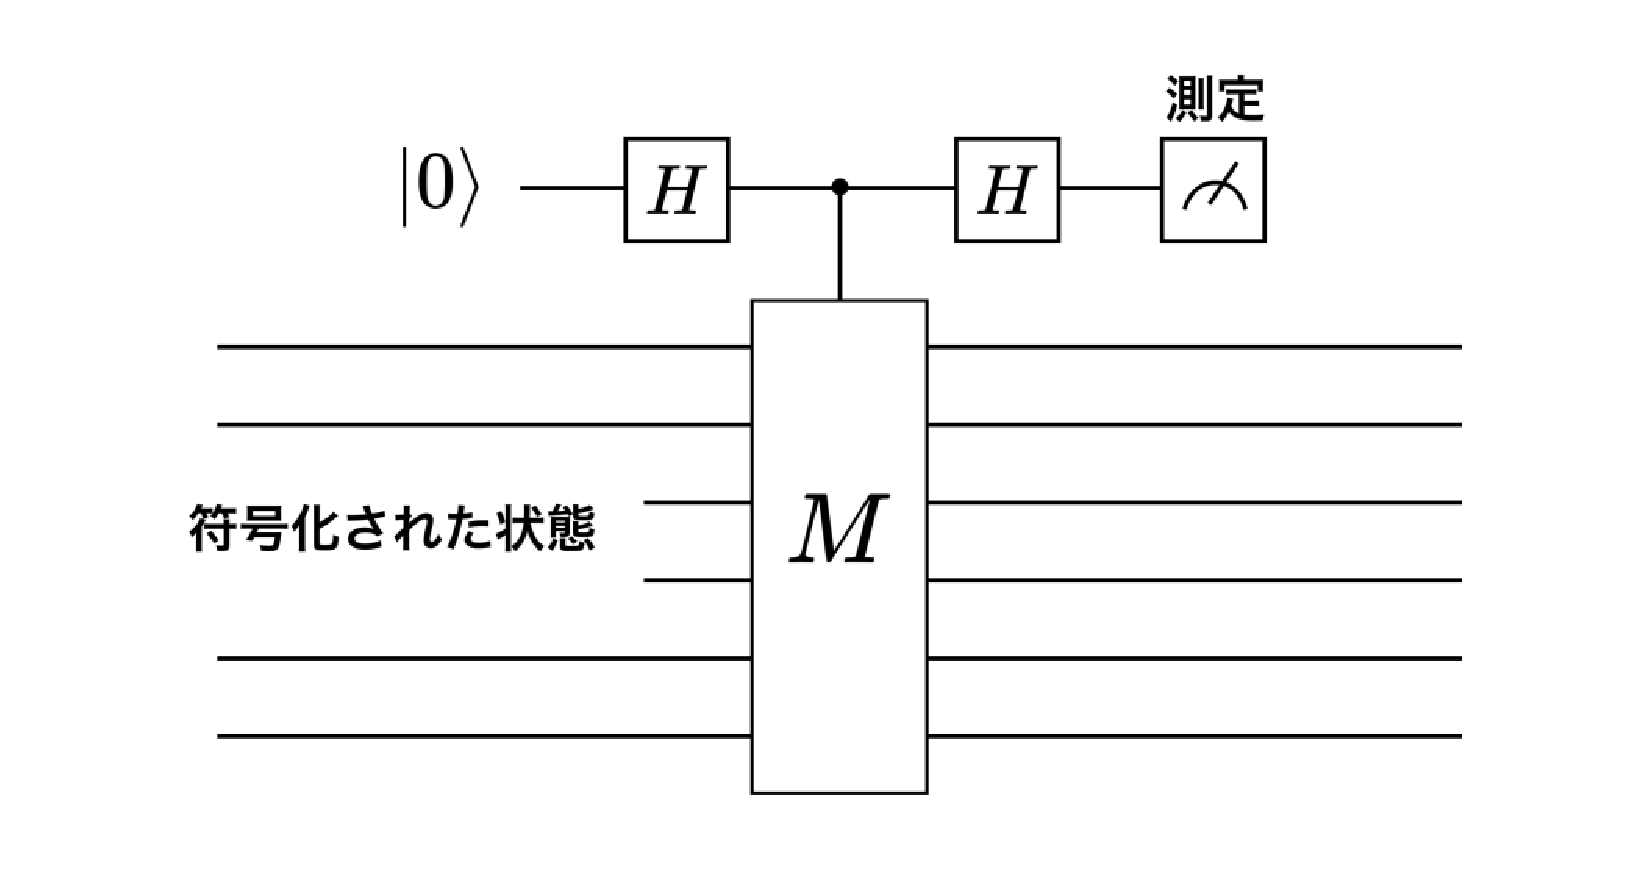
\includegraphics[width=0.8\linewidth]{error_obs.eps}
  \captionof{figure}{一般のシンドローム測定回路}
  \label{fig:stabilizer-circuit}
\end{center}
この時、終状態は以下のように記述される。
\begin{align*}
    \ket{f}&=\frac{1}{2}\ket{0}(\ket{\psi}_{L}+U\ket{\psi}_{L})+\frac{1}{2}\ket{1}(\ket{\psi}_{L}-U\ket{\psi}_{L})
\end{align*}
何もエラーが存在しなかったら、明らかにAncillaは0であり、stabilizer群と反可換なエラーが作用した場合はAncillaは1である。
\end{setupbox}
最後に、エラー訂正の手続きを述べる。
\begin{setupbox}{stabilizer符号のエラー訂正}
    エラー訂正は、逆操作によりなされる
\end{setupbox}
以上の手続きにより、一般のstabilizer群に対する「stabilizer符号」を確かに構成できた。

\subsubsection{誤り耐性をもつ演算}
前節までで、確かにstabilizer群を用いた符号である、stabilizer符号を構成することに成功した。ただし、前回行ったことは状態をエラーから守る方法を構築しただけであり、肝心の状態操作のことは一切考えられてなかった。この節では、状態操作を含めて、エラー訂正の構造を保つ方法を考察する。\\
\\
例えば、操作となるユニタリーゲートUが以下の性質を満たせば、その操作はエラー訂正の構造を保てることが主張できるであろう。
\begin{resultbox}{ユニタリーゲートUのエラー訂正可能性}
    あるユニタリーゲートUが以下の性質を満たすとする。
    \begin{align*}
        <U^{\dagger}g_{1}U,\cdots ,U^{\dagger}g_{k}U> \in \text{(stabilizer群)}
    \end{align*}
    この時、ユニタリーゲートU作用後のstateに対して、誤り検出回路を構築可能である。
\end{resultbox}
\begin{proofbox}
    stabilizer群,stabilizer状態を指定すれば誤り訂正可能であることは、前節で示した通りである。なおかつ、stabilizer形式を採用すると、ユニタリーゲートによりstabilizer群を更新することは示した通りである。\\
    \\
    故に、以下のチャートのようなセットアップを採用すれば、誤り訂正を行えることがすぐに理解できるであろう。\\
    \begin{figure}[h]
    \centering
    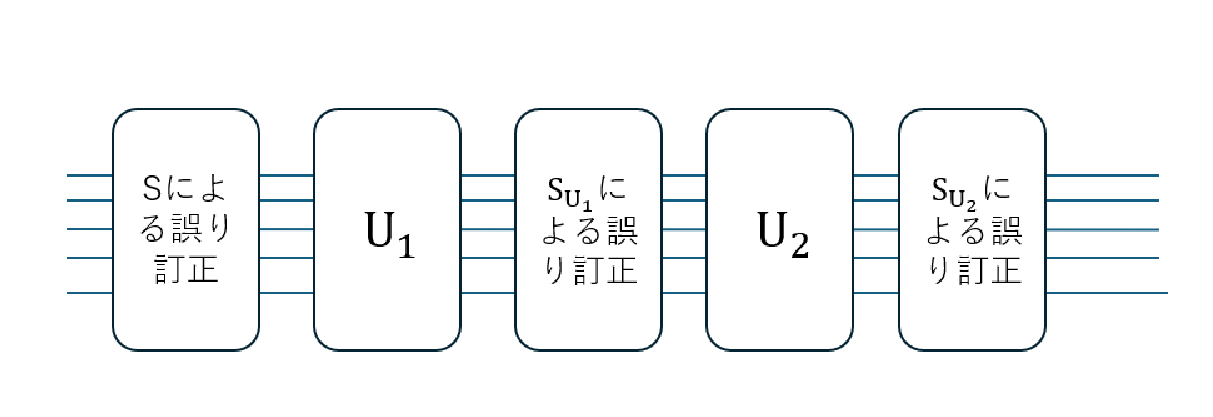
\includegraphics[scale=0.5]{stabilizer演算形式のエラー訂正.eps}
    \caption{エラー訂正回路}
    \label{fig_outlook}
    \end{figure}
\end{proofbox}
このようなユニタリーゲートUの集合を、「Clifford群」と呼ぶ。
\begin{defbox}{Clifford群}
    Clifford群とは、以下を満たすユニタリーゲートUの集合である。ただし、nビットパウリ群を$G_{n}$とする。
    \begin{align*}
        \text{(Clifford群)}=\{U\in \text{U(n)} |UgU^{\dagger}\in G_{n} (g\in G_{n})\}
    \end{align*}
    また、Clifford群に属したゲートのことを、「Cliffordゲート」としばし呼ぶ。
\end{defbox}
Cliffordゲートという言葉を用いるなら、先ほどのstatementは以下のように書き換えられるであろう。
\begin{resultbox}{CliffordゲートUのエラー訂正可能性}
    あるユニタリーゲートUが以下の性質を満たすとする（つまりユニタリーゲートがCliffordゲートであるとする）。
    \begin{align*}
        <U^{\dagger}g_{1}U,\cdots ,U^{\dagger}g_{k}U> \in \text{(stabilizer群)}
    \end{align*}
    この時、状態操作後のstateに対して、誤り検出回路を構築可能である。
\end{resultbox}
ただし、注意すべきことがある。ユニタリーゲートを作用させた後の群は、必ずしもstabilizer群になるとは限らない。これは、全てのユニタリーゲートがCliffordゲートではないことを意味する。\\
以下では、どのゲートがCliffordゲートであり、どのゲートが違うかの例を、いくつか挙げる。
\begin{resultbox}{Cliffordゲートの例}
\begin{align*}
    X,Y,Z,H,CNOT
\end{align*}
\end{resultbox}
\begin{proofbox}
    個別に作用させた場合のマップを確認すればよい。本証明では、特に非自明な結果である、CNOTゲートがstabilizer形式を保つことのみを、代表して示す。\\
    \\
    また簡単のため、stabilizer群ではなくPauli群でのマップを考察する。Pauli群で考えた後に可換な部分を取ってくるとstabilizer群になり、ユニタリ群の作用でstabilizerの構造は変わらないため、それで十分である。\\
    \\
    CNOTゲートは2ビット間の演算であるため、考えるべきPauli群は2ビットPauli群で十分である。また、ユニタリーゲートの作用を考えるため、全体の符号などは一切関係ない。故に、以下の生成子を持つ群への作用を考えれば十分である。
    \begin{align*}
        G=<X_{1},X_{2},Z_{1},Z_{2}>
    \end{align*}
    CNOTゲートの作用が上記のG内、もしくはその積に閉じていることを示せればよい。そしてそれを示すためには、全てのゲートを行列表示にしてそれを計算すればいいだけである。結果としては以下の通りである。
    \begin{align*}
        &(CNOT_{1,2})X_{1}(CNOT_{1,2})=X_{1}X_{2}\\
        &(CNOT_{1,2})X_{2}(CNOT_{1,2})=X_{2}\\
        &(CNOT_{1,2})Z_{1}(CNOT_{1,2})=Z_{1}\\
        &(CNOT_{1,2})Z_{2}(CNOT_{1,2})=Z_{1}Z_{2}
    \end{align*}
    故にCNOTゲートの作用で閉じているため、CNOTゲートはstabilizer形式を保つ。
\end{proofbox}
無論、ここで紹介したよりも多くのゲートが、Cliffordゲートであることは、個別に示していけばすぐにわかるであろう。\\
\\
反面、Cliffordゲートでない例としては以下が挙げられる。
\begin{resultbox}{Cliffordゲート「でない」例}
   \begin{align*}
        T,Toffoli
   \end{align*}
\end{resultbox}
\begin{proofbox}
例えばTゲートが違うことを示す。このためには、ただ単に1ビットのパウリ群にTゲートを作用させて、閉じないことを示せばよい。そのためには、以下を導出できれば十分である。
\begin{align*}
    TXT^{\dagger}=\frac{1}{\sqrt{2}}(X+Y)
\end{align*}
足し算は群の構成要素ではないため、確かにTゲートはstabilizer群の構造を保たないことがわかる。故にTゲートはCliffordゲートではない。
\end{proofbox}
無論、ここで紹介したよりも多くのゲートが、Cliffordゲートでないことは、個別に示していけばすぐにわかるであろう。
\subsubsection{Gottesmann-Knillの定理}
本小節で見たように、stabilizer符号は、量子誤り訂正符号を記述する上で極めて有用である。しかし一方で、stabilizer符号の誤り訂正能力を保つ、Clifford群による演算は、Tゲートなど明らかに使用できないゲートが存在するため、通常の量子計算よりも演算能力が低いのも想像がつくであろう。\\
この時、「stabilizer符号によって記述される量子状態や量子操作のみを用いた場合、量子優位性は存在しうるのか？」という疑問が自然に生じる。\\
\\
前節でみた通り、stabilizer状態に対して作用し、その構造を保つ演算としてCNOT演算が存在している。CNOTは量子もつれを生成するゲートであるため、ナイーブには、まだ強力な量子計算を実現できるように思われる。ところが、Gottesman-Knill の定理によって、以下の衝撃的な結果がもたらされた。
\begin{theorembox}{Gottesman-Knillの定理}
    Cliffordゲートのみの量子計算は、古典計算でシミュレーション可能である。
\end{theorembox}
これは、量子計算の計算能力が優位であるという主張が、如何に微妙であるかを示している。衝撃的な結果ではあるが、証明自体は単純である。
\begin{proofbox}
    量子計算が古典計算でシミュレーションできない理由は、例えばnビットの量子計算を古典計算を完全に記述するために、$O(2^{n})$ビットが必要であるためである。\\
    \\
    それに対し、Clifford演算が古典計算でシミュレーション可能であることを示すには、Clifford演算を記述するために必要な容量を計算すれば良い。\\
    そのためには、Clifford演算の記述方法である、stabilizer群を完全に記述するには何ビット用いるかを計算すればよい。nビットstabilizer群を記述するために必要な容量がnの多項式程度であれば、Gottesmann-Knillの定理が証明されたこととなる。\\
    \\
    k個の生成子からなるstabilizer群を記述した際、それで安定化される状態のなす空間は$2^{n-k}$次元である。故に、完全に状態を指定するためには、n個の生成子を用意したstabilizer群を用意すれば良い。
    \begin{align*}
        G_{n}=<g_{1},\cdots ,g_{n}>
    \end{align*}
   この時、生成子一つを記述するのに必要な古典ビット数がいくつかを計算する。stabilizer群の生成子は、一般的に以下の形に書ける。
   \begin{align*}
       g=X_{i}^{x_{i}}Z_{i}^{z_{i}}
   \end{align*}
   ただし、$x_{i},z_{i}$は、i番目のビットにX,Zがかかっているかを表す添字であり、$x_{i},z_{i}=0,1$である。\\
   \\
   stabilizer群の要素は$x_{i},z_{i}$を指定すれば、一意に定まる。そして$x_{i},z_{i}$を記述するには、1ビットが2n個分必要なだけなので、stabilizer生成子を一つ記述するのに必要なビット数は精々O(n)程度である。\\
   \\
   また、stabilizer生成子の数は精々n個である。ゆえに、stabilizer群全体を記述するのに必要な容量は、精々以下の通りである。
   \begin{align*}
       O(n)\times O(n)=O(n^{2})
   \end{align*}
   これはnビットのClifford演算を行うために必要なビット数がnの多項式程度でしかないことを意味する。故に、定理は示された。
\end{proofbox}
この定理に含まれている含蓄は、主に二つある。\\
\begin{enumerate}
    \item stabilizer形式にはCNOTやアダマールゲートが含まれているため、上記の主張を通せば、「量子もつれ」の存在をも古典でシミュレーション可能であること。故に、量子超越性に量子もつれの存在は、必要条件たり得ないということ。
    \item stabilizer形式を誤り耐性の方法論として採用した場合、量子優位性を保つ必要条件として、少なくともstabilizer形式の下「誤り耐性を持たない」ゲートを、どうにかして誤り訂正しながら用意しなければならないこと。この一見矛盾した要請が、量子誤り訂正の最大の課題である。次章では、これを破るためのアイデアを2つほど紹介する。
\end{enumerate}

\subsection{量子誤り訂正符号のエラー訂正能力}
今まででは、「こういった符号を考えるとこういったエラーが訂正できる」ということを、あくまで発見法的に示してきた。しかし、stabilizer符号といった構成論的に符号を構築する場合、どのようなエラーが訂正できるかを逐一探るのは、はっきりいって非効率であろう。ここではその壁を越えるべく、量子誤り訂正符号のエラー訂正能力の一般論を探ることを行う。



\section{量子誤り訂正の出口戦略}
量子誤り訂正理論の究極の目標は、有限のエラー率を持つ物理量子ビットのみを用いて、任意に長い量子計算を高い信頼性で実行できる誤り耐性量子コンピュータ（Fault-Tolerant Quantum Computation; FTQC）を実現することである。この目標が理論的に実現可能であることを保証するのが閾値定理であり、物理エラー率がある閾値以下であれば、誤り訂正符号を階層的に構成することで論理エラー率を任意に小さくできることが知られている。\\
\\
本章では、このFTQCを実現するための基礎理論として、まず古典誤り訂正との違いを整理し、量子誤り訂正の基本原理を導入する。その後、スタビライザー形式、閾値定理、magic state distillationといったFTQCを支える主要な概念について順に説明する。

\subsection{誤り耐性あり量子コンピュータ(FTQC)}
誤り耐性の究極目標は、現実的な確率で起こりうるあらゆるエラーを訂正することである。本節では、これを実現するために必要となる事項について紹介する。

\subsubsection{FTQCのゴール(閾値定理)}
量子誤り訂正理論の究極の目標は、量子コンピュータを実用的な計算機として成立させることである。そのためには、量子状態に生じる誤りを十分な精度で検出・訂正し、計算時間が長くなっても計算結果の信頼性を維持できなければならない。\\
この目標を達成するための最も素朴な発想は、「より多くの誤りを訂正できる符号を構築する」ことである。\\
\\
誤り訂正能力を向上させる機械的な方法論として、「符号の入れ子構造」というものを導入する。感覚を掴むため、X-flipエラーを訂正できる、3ビット符号を例としてみる。
\begin{setupbox}{3ビット符号の入れ子構造}
    真の物理量子ビットを、便宜上「0th量子ビット」と呼ぶことにする。\\
    この時、3ビット符号とは、0th量子ビット3つを束ね、3つのうち1つのX-flipエラーを訂正できる回路であることは、前述したとおりである。この符号化した「0th量子ビット」を用いて符号化した論理量子ビットのことを、「1st量子ビット」と呼ぶことにする。\\
     \begin{center}
    \centering
    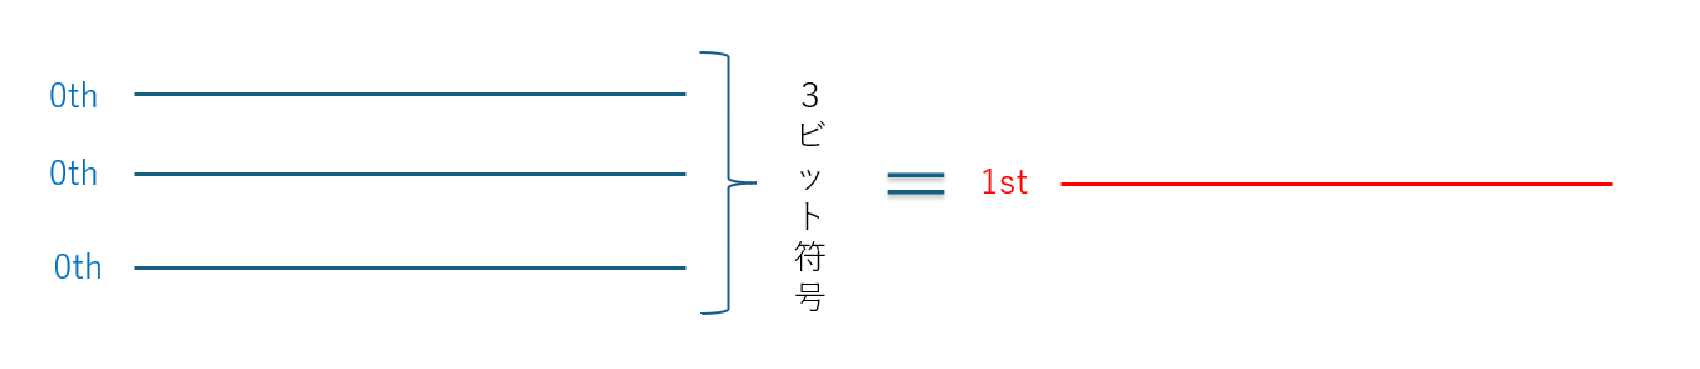
\includegraphics[scale=0.3]{first.eps}
    \captionof{figure}{3ビット符号(入れ子構造第１層)}
    \label{fig_outlook}
    \end{center}
    この時、自然に「第(n-1)th量子ビット」を物理量子ビットとして、論理量子ビットである「第nth量子ビット」を構成できる。このように、誤り訂正符号を束ねて、より大きな量子誤り訂正符号を構成できる構造のことを、「符号の入れ子構造」と呼ぶ。\\
    入れ子構造は量子回路図的には、以下のように記述できる。\\
    \begin{center}
    \centering
    \includegraphics[scale=0.3]{ladder.eps}
    \captionof{figure}{入れ子構造}
    \label{fig_outlook}
    \end{center}
\end{setupbox}
この符号の入れ子構造の第n層の量子誤り訂正の能力は、以下のような性質を持つことが知られている。
\begin{resultbox}{入れ子構造第n層の誤り訂正能力}
Assumption:\\
元々の符号の訂正能力が１個のspin-flip分である。\\
エラー伝搬が起こらない。\\
result:\\
入れ子構造第n層の符号の訂正できるspin-flip数を$a_{n}$とすると、以下のような漸化式が成立する。
\begin{align*}
    a_{n}=2(a_{n-1}+1)-1=2a_{n-1}+1
\end{align*}
故に、第n層の誤り訂正符号のエラー訂正能力は、大体以下のオーダーである。
\begin{align*}
    O(2^{n-1})
\end{align*}
\end{resultbox}
\begin{proofbox}
    訂正できなくなる最低のエラーの数を数える。\\
    \\
    第(n-1)層のspin-flip能力は、仮定より、$a_{n-1}$個である。この時、第n層でエラー訂正ができなくなるためには、(n-1)th量子ビットのうち２つが反転する必要がある。これが起こるためには、(n-1)th量子ビットがちょうど訂正できなくなるエラー、すなわち、$a_{n-1}+1$個のエラーが、２つの(n-1)-thビット分必要となる。すなわち、
    \begin{align*}
        \text{(第n-thで訂正できなくなるエラー数)}=2(a_{n-1}+1)
    \end{align*}
    これが、エラーが訂正できなくなる最小のエラー数である。これより１でも低ければ、エラーは必ず訂正できるため、訂正できるエラーの個数は、
    \begin{align*}
        a_{n}=2(a_{n-1}+1)-1=2a_{n-1}+1
    \end{align*}
    オーダー計算は上記の漸化式からすぐにわかる。
\end{proofbox}
これにより、確かにエラー訂正能力が向上することが理解できた。では、入れ子構造を採用すれば、現実的にエラーを訂正できる符号を構築できるのだろうか？\\
\\
しかし実際には、問題はそれほど単純ではない。例えば、物理量子ビットの数が増加すれば、それだけ系全体で誤りが発生する機会も増加する。また、符号化や誤り検出のためには多数の量子ゲートを実行しなければならないが、各ゲート自体も有限の誤差率を持つ。\\
\\
このことから、ナイーブには、ただ単にビット数を増やせば良いわけではなさそうである。では、誤り耐性を備えた量子コンピュータというゴールに向けて、我々はそもそも何を指針にするべきであろうか？\\
\\
しかし、実は上述のナイーブな直感こそ間違えていて、「ある条件」の下では、符号を入れ子構造で巨大化することが良い指針となるという結果が、実は知られている。このありがたい性質は、以下のような「閾値定理」として知られている\footnote{ただし、いくら入れ子構造でエラーを小さくできるからと言って、それで満足してはならない。量子計算の元々のモチベーションとして、「古典計算よりスケーリングのいい計算機」を作ることが挙げられたはずである。故に、入れ子構造の符号化の計算量を求め、改めて量子優位性を示さねば、最終的に満足のいく量子コンピュータとは言えない。この議題には本論では触れないが、結論としては、この誤り訂正符号の下でもちゃんと量子優位性が存在することが明らかとなっている。}。
\begin{theorembox}{閾値定理}
Assumption:\\
エラー伝搬が起こらない。\\
物理ビットにエラーが発生する頻度は一定。\\
result:\\
符号の入れ子構造を用いることにより、任意の精度でエラーを修復できる誤り訂正符号を構成することが可能である。
\end{theorembox}
\begin{proofbox}
    閾値定理を証明するためには、ある条件の下では、訂正できなくなるエラーが起きる確率を、任意に小さくできることを示せればよい。
    \begin{enumerate}
        \item 入れ子構造第0層\\
       この時、エラーが起こる確率をpとする。第０層ではエラーが起こると訂正できなくなるため、エラー発生率のオーダーは
       \begin{align*}
           O(p)
       \end{align*}
       \item 入れ子構造第1層\\
       物理ビット１つ1つのエラー発生率は変化しないが、「どれか一つの量子ビットへのエラーの発生率」は、量子ビットの数だけ、組み合わせ論的に増加する。この冗長化に伴うエラーの起きやすさの補正をCとする\footnote{3ビット符号の場合、3通り存在するため、おそらくC=3?}。この場合、エラーが2個以上起きると、論理エラーになるため、エラー発生率は、
       \begin{align*}
           O(Cp^{2})
       \end{align*}
       \item 入れ子構造第２層\\
       論理ビットから論理ビットに行く際のエラー起こりやすさの補正を考える。\\
       エラーが発生する条件は、論理ビットのいずれか2つの反転であるため、組み合わせ論の補正をCとすると、エラー発生確率は$\text{(論理Flip２つの発生確率)}\times\text{(どこで起きるかの組み合わせ)}$である。前者は前に与え、後者はCそのものであるため、エラー発生率は、
       \begin{align*}
           O((Cp^{2})^{2}C)
       \end{align*}
       \item 入れ子構造第n層\\
       第２層以上は同じ構造であるため、繰り返すと、エラー発生率は
       \begin{align*}
           O(\frac{(Cp)^{2n}}{C})
       \end{align*}
    \end{enumerate}
    入れ子構造から作られる符号におけるエラー発生率が求まったので、後はこれがnの増加とともに減少する条件を考える。これは非常に単純で、
    \begin{align*}
        Cp<1 \iff p<p_{th}\equiv \frac{1}{C}
    \end{align*}
    である。故に、閾値$p_{th}=\frac{1}{C}$よりエラー率が低ければ、入れ子構造を採用することにより、任意の精度でエラー発生率を減少させられる。
\end{proofbox}
この閾値定理は、指数の肩の係数依存性以外に符号の詳細によらない。当然、古典や量子にもよらない。そのため、量子誤り訂正符号にも応用可能である。

\subsubsection{エラー伝播}
我々は前章までで、FTQCを満たすためには何がゴールであるかを、「ある仮定が成立する条件の下で」示した。その仮定を再掲すると、
\begin{enumerate}
    \item エラー伝搬が起こらない。
    \item 物理ビットにエラーが発生する頻度は一定。
\end{enumerate}
後者の条件は、現状では実験家の人たちに頑張ってもらうしかないように思える。しかし、前者の「エラー伝搬」が起こらないような冗長化を考えるのは、我々が介入する余地があるのではないかと思える。\\
\\
まずは、エラーを致命的に増幅させうる「エラー伝播」の概念をよく知らなければならない。エラー伝播とは、一つのエラーが量子回路の中で増幅され、複数ビットに跨るようなエラーとなる現象である。感覚を掴むため、まず例として、非常に簡単な回路を構築し、エラー伝播を体験してみるのが一番であろう。以下のようなモデルとなる回路を考える。\\
\begin{center}
    \centering
    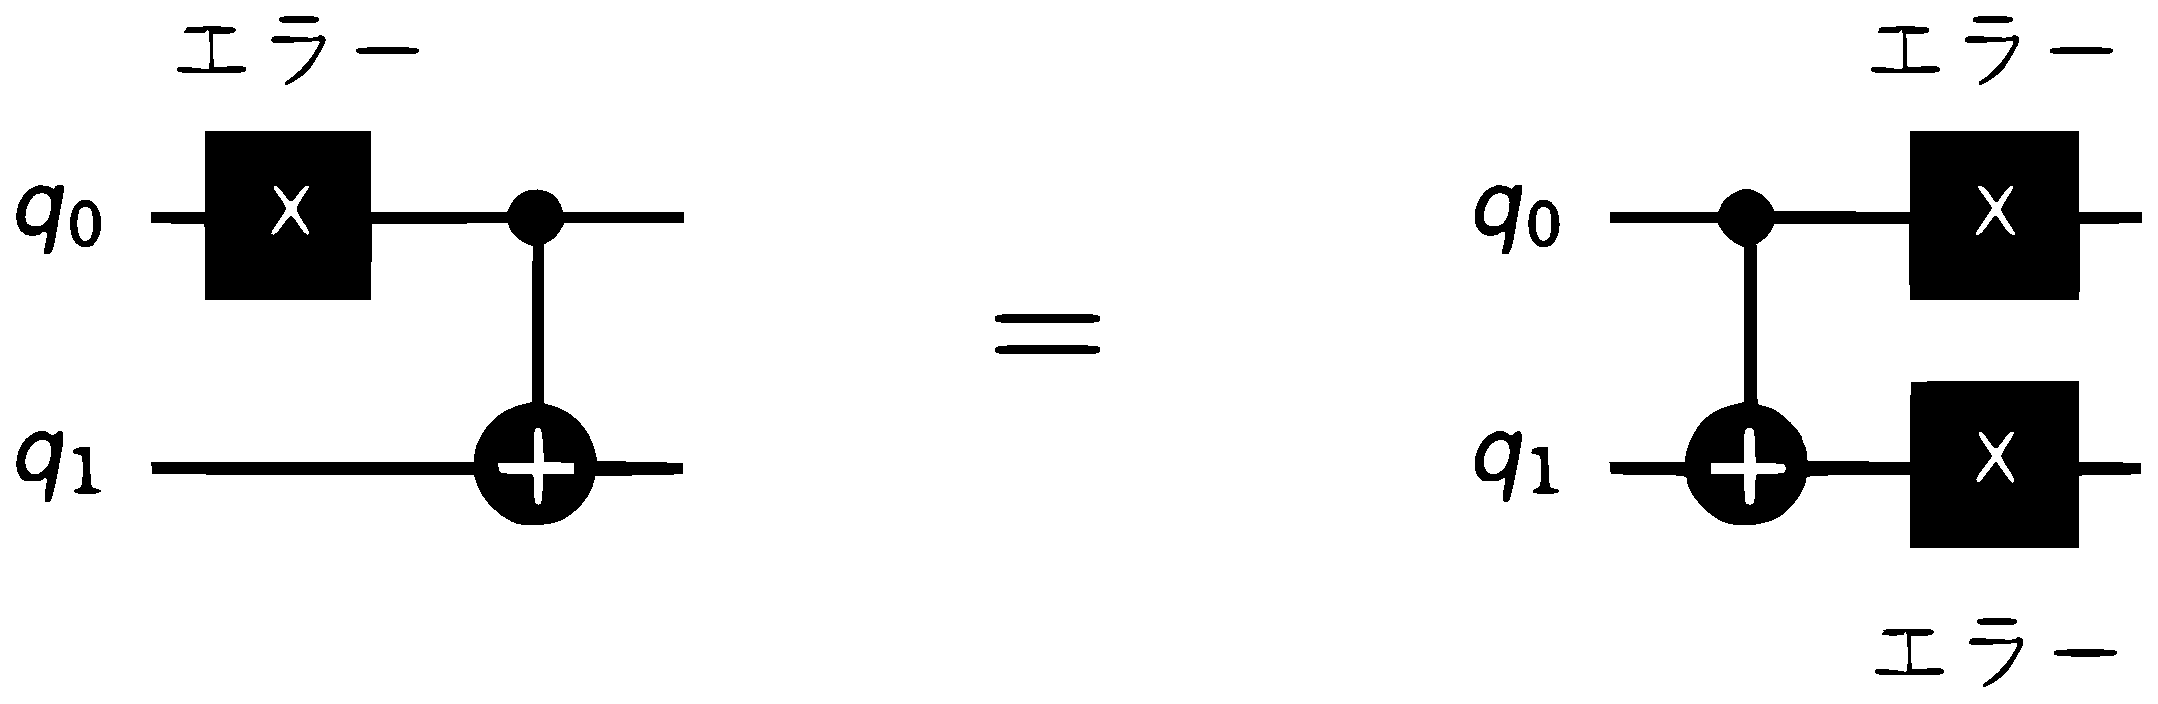
\includegraphics[scale=0.3]{error_propagate.eps}
    \captionof{figure}{エラー伝搬の模式図}
    \label{fig_outlook}
    \end{center}
図の左側は、Xゲートでエラーが張られている様子を表している。また、図の左側は、CNOTゲートを介することで、1つのエラーが2つのエラーに増幅されている様子を表している。\\
この図の通り、CNOTゲートの作用により、1つしか存在しないはずのエラーが、2つ以上に伝搬・増幅される。この現象のことを、「エラー伝搬」と呼ぶ。これにより、本来確率$O(p^{2})$でしか起きないはずの2つ以上のエラーが、伝搬の効果によりO(p)程度の確率で起こることになり、それ故、前回の閾値定理の証明が破綻する、というのが、エラー伝搬が致命的となる由来である。


\subsubsection{エラー伝播のない量子コンピュータ実現のために}
上記のエラー伝播の本質は、「CNOTを通じてエラーが拡大すること」であった。故に、エラー伝播のない誤り訂正符号を構築しようと思うなら、「CNOTゲートができる限り１対１となる」ような訂正符号を構築すればいいであろう。\\
\\
一つの量子ビットに複数のCNOTが作用される代表的な場所が、「エラーを探るAncillaと、論理ビットの間」である。この問題を解決するためには、ancillaとして、符号と同程度の量のancillaを検出用のビットとして用意し、各物理ビットと1:1となるように、CNOTをつなげば、例えば良いことがわかる。
\subsubsection{エラーに強い観測}
誤り訂正の枠組みではエラーの検出、訂正を行うのが常道ではあるが、その際、観測はエラーなしで起こるというのが前提であった。しかし、現実問題として、観測でも普通にエラーが起こりうる。\\
\\
そこでエラーに強い観測が必要になるが、そのための方法論として単純に考えられるのは、「観測を繰り替えす」ことである。こうすることで、個々の観測にエラーが起きても、平均を取ればエラーのない結果が得られるという寸法である。

\subsection{Cliffordを超えた演算}
前章では、Gittesmann-Knillの定理より、Cliffordゲートを用いた誤り訂正を確保した量子コンピュータは、何ら量子優位性を持たないことを示した。この定理より、真に量子優位性を持つ計算をFault-tolerantに行うためには、Clifford群に属さないゲートをエラー訂正できるように実装しなければならない。\\
\\
この実装を行う際に、非常に重要な事象を一つ告げねばならないだろう。先ほどCliffordゲートに対して述べたstatementを再掲する。
\begin{resultbox}{CliffordゲートUのエラー訂正可能性}
    あるユニタリーゲートUが以下の性質を満たすとする（つまりユニタリーゲートがCliffordゲートであるとする）。
    \begin{align*}
        <U^{\dagger}g_{1}U,\cdots ,U^{\dagger}g_{k}U> \in \text{(stabilizer群)}
    \end{align*}
    この時、状態操作後のstateに対して、誤り検出回路を構築可能である。
\end{resultbox}
他の教科書ではあまりちゃんと強調しないが、あくまでこれは十分条件である。故に、実はT-ゲートをエラー訂正可能性を保ったまま実装する方法を行うことは、「理論上」可能である、ということが、告げるべき事象である。\\
\\
例えば、ロジカルTゲートを以下のようなものと定義すれば、実質的にTゲートは誤り訂正の構造を保ちつつ実装可能である。
\begin{setupbox}{ロジカルTゲートの誤り訂正可能性}
あるstabilizer群に対する符号空間を、以下のように設定する。
\begin{align*}
    <\ket{0}_{L},\ket{1}_{L}>
\end{align*}
この時、ロジカルT-ゲート$T_{L}$を、以下のように作用するオペレータと定義する。
\begin{align*}
    &T\ket{0}_{L}=\ket{0}_{L}\\
    &T\ket{1}_{L}=e^{i\frac{\pi}{4}}\ket{1}_{L}
\end{align*}
この場合、符号空間内のstate$\ket{\psi}=a\ket{0}_{L}+b\ket{1}_{L}$にロジカルTゲートを作用した後のstateは、符号空間内に留まり続けることが、以下のように理解できる。
\begin{align*}
    S(T\ket{\psi})&=S(a\ket{0}_{L}+be^{i\frac{\pi}{4}}\ket{1}_{L})\\
    &=a\ket{0}_{L}+be^{i\frac{\pi}{4}}\ket{1}_{L}\\
    &=T(a\ket{0}_{L}+b\ket{1}_{L})\\
    &=T\ket{\psi}
\end{align*}
故に、ロジカルTゲートを作用させた後のstateに対しても、誤り検出回路を構築可能である。
\end{setupbox}
ただし、Clifford群の場合とは異なり、ロジカルTゲートをCliffordゲートと同様の方法でFault-tolerantに実装することは一般には困難である。\\
\\
しかし、その後の研究により、ロジカルTゲートの実装過程で一時的にstabilizer構造を失ったとしても、それ自体は必ずしも致命的ではないことが明らかとなった。\\
この考え方に基づく代表的な手法が「magic state injection」及び「magic state蒸留」である。以下でその概要を紹介する。\\
\\
なお、この方法は途中でCliffordの構造を捨てており、Gottesmann-Knillの定理の制限を逃れているため、量子優位性の必要条件は満たしているということを最初に明記しておく。それでいて尚且つ、誤り訂正の構造そのものは保っているのが、このアイデアの面白いところである。
\subsubsection{magic-state injection}
最初に、Tゲートの実相において核となるアイデアである「ゲートテレポーテーション」という現象について説明する。\\
ゲートテレポーテーションとは、実装の難しいゲートを、量子テレポーテーションを用いて、間接的に実装しようというアイデアである。以下で、例としてXゲートのテレポーテーションを述べる。
\begin{examplebox}{Xゲートテレポーテーション}
    まず、実装したい入力状態を
\begin{align*}
    \ket{\psi}=a\ket{0}+b\ket{1}
\end{align*}
とする。ここで、あらかじめ以下のような補助状態を用意しておく。
\begin{align*}
    \ket{\Phi_X}
    =
    (I\otimes X)\frac{1}{\sqrt{2}}(\ket{00}+\ket{11})
    =
    \frac{1}{\sqrt{2}}(\ket{01}+\ket{10})
\end{align*}
これは、通常のBell対の片側にあらかじめ \(X\) ゲートを作用させた状態である。\\
\\
このとき、入力状態 \(\ket{\psi}\) と補助状態 \(\ket{\Phi_X}\) を合わせた状態は
\begin{align*}
    \ket{\psi}\ket{\Phi_X}
    =
    (a\ket{0}+b\ket{1})
    \frac{1}{\sqrt{2}}(\ket{01}+\ket{10})
\end{align*}
である。ここで、入力状態と補助状態の片方のビットに対してBell測定を行う。Bell基底は
\begin{align*}
    \ket{\Phi^{+}}&=\frac{1}{\sqrt{2}}(\ket{00}+\ket{11}),&
    \ket{\Phi^{-}}&=\frac{1}{\sqrt{2}}(\ket{00}-\ket{11}),\\
    \ket{\Psi^{+}}&=\frac{1}{\sqrt{2}}(\ket{01}+\ket{10}),&
    \ket{\Psi^{-}}&=\frac{1}{\sqrt{2}}(\ket{01}-\ket{10})
\end{align*}
である。この基底で展開すると、
\begin{align*}
    \ket{\psi}\ket{\Phi_X}
    =
    \frac{1}{2}\Big[
    &\ket{\Phi^{+}}\,X\ket{\psi}
    +\ket{\Phi^{-}}\,XZ\ket{\psi} \\
    &+\ket{\Psi^{+}}\,\ket{\psi}
    +\ket{\Psi^{-}}\,Z\ket{\psi}
    \Big]
\end{align*}
となる。\\
\\
したがって、Bell測定の結果に応じて、第3量子ビットには以下の状態が残る。
\begin{align*}
    \Phi^{+}&:\quad X\ket{\psi},\\
    \Phi^{-}&:\quad XZ\ket{\psi},\\
    \Psi^{+}&:\quad \ket{\psi},\\
    \Psi^{-}&:\quad Z\ket{\psi}.
\end{align*}
測定結果に応じてPauli補正を行えば、最終的に常に
\begin{align*}
    X\ket{\psi}
\end{align*}
を得ることができる。\\
\\
つまり、直接 \(X\) ゲートを入力状態に作用させる代わりに、あらかじめ \(X\) ゲートを作用させたBell対を用意し、Bell測定とPauli補正を行うことで、\(X\) ゲートをテレポートできる。
\end{examplebox}
以下では、このゲートテレポーテーションのアイデアを用いて、「magic state$\ket{T}$」が用意できた場合に、TゲートをFault-tolerantに実装できる、「magic state injection」と呼ばれるアイデアを説明する。ここでの説明は、Bravyi–Kitaev の原論文に沿うので、教科書的な説明とは少し違うかもしれない。
\begin{setupbox}{magic-state injection}
まず、以下の「magic-state」と呼ばれる状態が用意できたとする。
\begin{align*}
    \ket{T}\equiv \frac{1}{\sqrt{2}}(\ket{0}+e^{i\theta}\ket{1})
\end{align*}
これと1ビットstate$\ket{\psi}=a\ket{0}+b\ket{1}$の間にCNOTゲートを作用させる。
\begin{align*}
    CNOT_{1,2}(\ket{T}\ket{\psi})=\frac{1}{\sqrt{2}}\ket{0}(a\ket{0}+be^{i\theta}\ket{1})+\frac{1}{\sqrt{2}}\ket{1}(ae^{i\theta}\ket{1}+b\ket{0})
\end{align*}
この際、量子ビット1に対して、$\sigma_{z}$の固有値の値を見るような観測を考える。その際、観測値の値により、観測後のstate$\ket{f}$は以下のように変わる。
\begin{align*}
    \text{(観測値+1)}&:\ket{f}=a\ket{0}+be^{i\theta}\ket{1}=R_{z}(\frac{\theta}{2})\ket{\psi}\\
    \text{(観測値-1)}&:\ket{f}=ae^{i\theta}\ket{1}+b\ket{0}=XR_{z}(-\frac{\theta}{2})\ket{\psi}
\end{align*}
Tゲートは$R_{z}(\frac{\theta}{2})$の特別バージョンであるため、観測値が+1であった場合に、magic stateを用いてゲートテレポーテーションによるT-ゲートの実装が行えた。この手続きが「magic-state injection」である。\\
\\
また、この回路ではパウリ行列の観測とCNOTゲートしか用いていないため、Fault-tolerantである。
\end{setupbox}
この手続きにより、magic-stateが「Fault-torelant」に用意できたとすると、T-ゲートを用いた手続きが「Fault-torelant」に行えることが可能となる。故に、後はmagic-stateの準備さえ完了すれば、ユニバーサルな量子計算を行うための必要事項が完了したことになる。
\subsubsection{magic-state蒸留}
以下では、magic-stateを用意する方法を考える。しかし、Fault-tolerantに直接生成する方法は、少なくとも2026年現在知られていない。「magic-state蒸留」は、エラーをある程度許容しつつ、質の高いmagic stateを大量に用意する方法である。\\
\\
magic-state蒸留のアイデアは、「誤りをある程度許容してmagic-stateの種を大量にばらまきつつ、Fault-tolerantに蒸留をすることでエラーの無いmagic stateを取り出す」というものである。まずは第一段階として、このアイデアが実現可能であることを示す。\\
\\
その前に、まずはmagic-stateの線形代数的な特性を述べる。
\begin{resultbox}{magic-stateの線形代数的性質}
    \begin{enumerate}
        \item magic-stateは、以下の行列Mの固有状態である。
        \begin{align*}
            M=\frac{e^{\frac{i\pi}{4}}}{\sqrt{2}}\begin{pmatrix}
         1 & 1 \\i& -i 
        \end{pmatrix}
        \end{align*}
        \item 行列Mのパウリ行列との交換関係
        \begin{align*}
        M^{\dagger}\sigma^{x}M=\sigma^{z},M^{\dagger}\sigma^{z}M=\sigma^{y},M^{\dagger}\sigma^{y}M=\sigma^{x},
        \end{align*}
        \item M行列の固有ベクトル\\
        M行列の固有ベクトルは、magic-stateの他に以下が存在する。
        \begin{align*}
            \ket{T_{1}}\equiv \sigma^{y}H\ket{T}
        \end{align*}
    \end{enumerate}
\end{resultbox}
\begin{proofbox}
    証明はただの線形代数の計算なので省略
\end{proofbox}
ただし、原論文ではT行列と書いてるところを、T-ゲートとの混同を避けるため、ここでは行列Mと記述した。\\
\\
ここで実際に、「5ビット分のエラーを含んだmagic-stateから、1ビットの、限りなく純粋なmagic-stateを取り出す」プロトコルとして、以下のセットアップを考える。
\begin{setupbox}{5ビットのmagic-state蒸留}
 ここから先しばらく、以下のような記法を用いる。
 \begin{align*}
     \ket{T_{0}}&\equiv  \ket{T}\\
     |x|&=(x^{1}+x^{2}+x^{3}+x^{4}+x^{5})\\
     \ket{T_{x}}&\equiv  \ket{T_{x_{1}}}\cdots\ket{T_{x_{5}}}
 \end{align*}
    \begin{enumerate}
        \item 初期状態の用意\\
        第一段階では、「誤りを許容してT-ゲートを用意する」ことを考える。この段階でGottesmann-Knillの制約からは逃れている。\\       \\
        簡単のため、以下のような状態を用意できたと考える。
        \begin{align*}
            \rho=(1-e)\ket{T}\bra{T}+e\ket{T_{1}}\bra{T_{1}}
        \end{align*}
        これは、エラー率eでmagic stateを導入することに等しい。\\
        \\
        これを５つ並べた以下のstateを、初期状態とする。
        \begin{align*}
            \rho_{in}=\sum_{x\in \{0,1\}^{5}}e^{|x|}(1-e)^{5-|x|}\ket{T_{x}}\bra{T_{x}}
        \end{align*}
        \item シンドローム測定\\
        以下のようなstabilizer生成子を考える。
        \begin{align*}
            S^{1}&=\sigma_{x}\otimes \sigma_{z}\otimes\sigma_{z}\otimes \sigma_{x}\otimes I_{2}\\
            S^{2}&=I_{2}\otimes\sigma_{x}\otimes \sigma_{z}\otimes\sigma_{z}\otimes \sigma_{x}\\
            S^{3}&=\sigma_{x}\otimes I_{2}\otimes\sigma_{x}\otimes \sigma_{z}\otimes\sigma_{z}\\
            S^{4}&=\sigma_{z}\otimes \sigma_{x}\otimes I_{2}\otimes\sigma_{x}\otimes \sigma_{z}
        \end{align*}
        シンドローム測定は、上記の生成子の固有値を計測することに相当する。
        \\
        またこの際、ロジカルMゲートを以下のように定義する。これの固有基底を用いるのが、蒸留の手続きを考える際に非常に便利である。
         \begin{align*}
            &M_{L}\equiv M\otimes \cdots \otimes M
        \end{align*}
        シンドローム測定後、「自明な結果が出た場合」、状態はロジカルMゲートの固有状態$\ket{T}_{L},\ket{T_{1}}_{L}$を用いて以下のように記述できる。
        \begin{align*}
            \rho_{s}=\frac{e^{5}+5e^{2}(1-e)^{3}}{6}\ket{T}_{L}\bra{T}_{L}+\frac{(1-e)^{5}+5e^{3}(1-e)^{2}}{6}\ket{T_{1}}_{L}\bra{T_{1}}_{L}
        \end{align*}
        自明な結果が出る確率は、上記より
        \begin{align*}
            p=\frac{e^{5}+5e^{2}(1-e)^{3}+(1-e)^{5}+5e^{3}(1-e)^{2}}{6}
        \end{align*}
        自明でない結果が出た場合、失敗したと判断し、捨てる。
        \item decoding(Encodingの逆操作)\\
        decode操作は、以下の3段階によりなされる。\\
        (i)以下で定義される操作Vを行う。
        \begin{align*}
            V:\text{(符号空間)}\to C^{2}\otimes \ket{0000} 
        \end{align*}
        (ii)$\ket{T},\ket{T_{1}}$を入れ替えるオペレータ、$\sigma^{y}H$を作用させる。\\
        (iii)第２から第５ビットに対し部分トレースを取ることにより、decode操作は完了。
        \item 蒸留終了\\
        終状態は、以下のように記述できる。
        \begin{align*}
            \rho_{f}=\rho=(1-e_{out})\ket{T}\bra{T}+e_{out}\ket{T_{1}}\bra{T_{1}}
        \end{align*}
        ただし、$e_{out}$は以下の通りである。
        \begin{align*}
            e_{out}=\frac{t^{5}+5t^{2}}{1+5t^{2}+5t^{3}+t^{5}},\quad t=\frac{e}{1-e}
        \end{align*}
    \end{enumerate}
以上で用いた操作はパウリ群の観測とCliffordゲートのみである。故に、最初のエラー許容のステップを除くと、すべての操作はFault-tolerantである。
\end{setupbox}
\begin{proofbox}
ここでは上のセットアップの時に省いた、細かい数式を追って、セットアップの主張が定量的に正しいことを導く。式変形を省いたのは主に2,3の手順であるため、そこを追っていく。
\begin{enumerate}
    \item シンドローム測定の式変形\\
    ここでのゴールは、以下を導くことである。
     \begin{align*}
            \rho_{s}=\frac{e^{5}+5e^{2}(1-e^{3})}{6}\ket{T_{0}}_{L}\bra{T_{0}}_{L}+\frac{(1-e)^{5}+5e^{3}(1-e^{2})}{6}\ket{T_{1}}_{L}\bra{T_{1}}_{L}
    \end{align*}
    これを書くためには、初期状態に対し、符号空間へmapするようなProjection$\Pi$の当たり方を考えれば良い。$\Pi$の表式は以下の通りである。
        \begin{align*}
            \Pi\equiv(\frac{1+S^{1}}{2})\cdots(\frac{1+S^{4}}{2})
        \end{align*}
    これの初期状態への当たり方をみるための道具を、いくつか見繕う。\\
    \\
    Projectionと可換な演算子として、以下のロジカルオペレータが挙げられる。
        \begin{align*}
            &M_{L}\equiv M\otimes \cdots \otimes M\\
            &X_{L}\equiv X\otimes \cdots \otimes X\\
            &Y_{L}\equiv Y\otimes \cdots \otimes Y\\
            &Z_{L}\equiv Z\otimes \cdots \otimes Z
        \end{align*}
    この時、明らかにロジカルオペレータたちは、以下の関係を満たす。
    \begin{align*}
    M^{\dagger}\sigma^{x}M=\sigma^{z},M^{\dagger}\sigma^{z}M=\sigma^{y},M^{\dagger}\sigma^{y}M=\sigma^{x}
    \end{align*}
    また、$M_{L}$は$\ket{T_{x}}$に対して、定義より明らかに、以下のように作用する。
    \begin{align*}
        M_{L}\ket{T_{x}}=e^{i\frac{\pi}{3}(5-2|x|)}\ket{T_{x}}
    \end{align*}
    これと$M_{L}$がProjectionと可換であるという性質を踏まえると、stabilizer群の符号空間内で、$M_{L}$の固有状態は、以下のように記述できる\footnote{ここで$\sqrt{6}$は規格化定数である。なぜこうであるかは、ここでしか使わない計算なので省略する。知りたいなら原論文Appendixを当たってほしい。}。
    \begin{align*}
        &\ket{T_{0}}_{L}\equiv \sqrt{6}\Pi \ket{T_{11111}}\\
        &\ket{T_{1}}_{L}\equiv \sqrt{6}\Pi \ket{T_{00000}}
    \end{align*}
    符号空間は2次元なので、符号空間内の任意のstateはこれらの線形結合でかける。\\
    密度行列表示では以下のように記述可能である。
    \begin{align*}
        &\ket{T_{0}}_{L}\bra{T_{0}}_{L}=\Pi \frac{1}{2}[I+X_{L}+Y_{L}+Z_{L}]\\
        &\ket{T_{1}}_{L}\bra{T_{1}}_{L}=\Pi \frac{1}{2}[I-X_{L}-Y_{L}-Z_{L}]
    \end{align*}
    またこの時、$M_{L}$に対するそれぞれの固有値は、以下の通りである。
    \begin{align*}
        &M_{L}\ket{T_{0}}_{L}=e^{-i\frac{\pi}{3}}\ket{T_{0}}_{L}\\
        &M_{L}\ket{T_{1}}_{L}=e^{i\frac{\pi}{3}}\ket{T_{1}}_{L}\\
    \end{align*}
    以上を踏まえて、Projectionを各stateに作用させたものが、どのような振る舞いをするかを考える。このためには、Projectionを作用させた後の$M_{L}$の固有値を調べ、そこから作用後の状態を類推してやればいい。
    \footnote{Projectionの作用から、$\Pi\ket{T_{x}}$が符号空間内に存在するのは明らかであるし、また$M_{L}$の固有状態であることも明らかなので、固有値から状態を特定可能である}。
    類推の結果は以下の通りである
    \footnote{結果についていくつか補足をしておく。
    ($|x|=1,4$)での結果は、$M_{L}$を作用させた際の固有値が$\pm 1$となることに由来する。これで尚且つ符号空間であることを考えると、ありうる選択肢は0のみである。($|x|=2,3$)での結果は、固有値は決まるけど、phaseや重みまで決まらないことに由来する。}。
    \begin{align*}
        \Pi\ket{T_{x}}=
        \begin{cases}
        \frac{1}{\sqrt{6}}\ket{T_{1}}_{L}\quad (|x|=0)    \\
        0  \quad (|x|=1)\\
        a_{x}\ket{T_{1}}_{L}\quad (|x|=2)    \\
        b_{x}\ket{T_{1}}_{L}\quad (|x|=3)    \\
        0\quad (|x|=4)    \\
        \frac{1}{\sqrt{6}}\ket{T_{1}}_{L}\quad (|x|=5)    
        \end{cases}
    \end{align*}
    故に、Projectionを作用させた密度行列は、以下の通りとなる。
    \begin{align*}
        \rho_{s}=\Pi \rho_{in} \Pi^{\dagger} 
        &=(\frac{e^{5}}{6}+e^{2}(1-e^{3})\sum_{|x|=2}|a_{x}|^{2})\ket{T}_{L}\bra{T}_{L}\\
        &+(\frac{(1-e)^{5}}{6}+e^{3}(1-e^{2})\sum_{|x|=3}|b_{x}|^{2})\ket{T_{1}}_{L}\bra{T_{1}}_{L}
    \end{align*}
    $\sum_{x}|a_{x}^{2}|,|b_{x}^{2}|$の値は以下の高等式に代入することで理解できる。
    \begin{align*}
        &\ket{T_{0}}_{L}\bra{T_{0}}_{L}+\ket{T_{1}}_{L}\bra{T_{1}}_{L}=\Pi(\ket{T_{0}}_{L}\bra{T_{0}}_{L}+\ket{T_{1}}_{L}\bra{T}_{L})\Pi=\Pi\\
    &\implies \sum_{x}|a_{x}^{2}|=\sum_{x}|b_{x}^{2}|=\frac{5}{6}
    \end{align*}
    以上をすべて踏まえると、Projection作用後のstateを以下として導ける。
     \begin{align*}
            \rho_{s}=\frac{e^{5}+5e^{2}(1-e)^{3}}{6}\ket{T_{0}}_{L}\bra{T_{0}}_{L}+\frac{(1-e)^{5}+5e^{3}(1-e)^{2}}{6}\ket{T_{1}}_{L}\bra{T_{1}}_{L}\\
    \end{align*}
    \item decodingの式変形\\
    ここでのゴールは、$\rho_{f}$の再現である。このために、Vの具体的な形を特定し、順次作用させることを考える。\\
    \\
    まず、「規格化された測定後状態」にキチンと修正する。規格化は測定確率pで状態を破ればいいので、規格化した測定後状態は以下のように記述される。
    \begin{align*}
        \rho_{s}^{reg}=&\frac{e^{5}+5e^{2}(1-e)^{3}}{e^{5}+5e^{2}(1-e^{3})+(1-e)^{5}+5e^{3}(1-e^{2})}\ket{T_{0}}_{L}\bra{T_{0}}_{L}\\
        &+\frac{(1-e)^{5}+5e^{3}(1-e)^{2}}{e^{5}+5e^{2}(1-e^{3})+(1-e)^{5}+5e^{3}(1-e^{2})}\ket{T_{1}}_{L}\bra{T_{1}}_{L}\\
        &=\frac{t^{5}+5t^{2}}{t^{5}+5t^{2}+1+5t^{3}}\ket{T_{0}}_{L}\bra{T_{0}}_{L}+\frac{1+5t^{3}}{t^{5}+5t^{2}+1+5t^{3}}\ket{T_{1}}_{L}\bra{T_{1}}_{L}\\&\quad\quad\quad\quad(t\equiv \frac{e}{1-e})\\
        &=\sqrt{1-e_{out}^{2}}\ket{T_{0}}_{L}\bra{T_{0}}_{L}+e_{out}\ket{T_{1}}_{L}\bra{T_{1}}_{L} 
    \end{align*}
    Decodeは、以下のようなstabilizer群の変更により行われる。
    \begin{align*}
        <S_{1},\cdots S_{4}>\implies<Z_{2},\cdots, Z_{5}>
    \end{align*}
    この変更を与える代表的なdecode操作として、「$Z_{2},\cdots, Z_{5}$基底による観測」が考えられる。これらの操作はいずれかのstabilizer群と反可換なので、確かにstabilizer群を変化させる。\\
    \\
    この測定に対する$\ket{T_{0,1}}_{L}$の変化を考える。Z基底の射影オペレータを実際にかけてみると、各stateは以下の通りとなる。
    \begin{align*}
        &\Pi_{z_{2}\cdots z_{5}}\ket{T_{0}}_{L}=\ket{T_{1}}\otimes \ket{0000}\\
        &\Pi_{z_{2}\cdots z_{5}}\ket{T_{1}}_{L}=\ket{T_{0}}\otimes \ket{0000}
    \end{align*}
    故に、$\ket{T_{0}},\ket{T_{1}}$を反転するようなオペレータをかけて、第２から第５ビットをトレースアウトすると、終状態は、以下のように記述できる。
        \begin{align*}
            \rho_{f}=\rho=(1-e_{out})\ket{T}\bra{T}+e_{out}\ket{T_{1}}\bra{T_{1}}
        \end{align*}
\end{enumerate}
これらの計算より、magic-state蒸留のセットアップは、確かに正しいことが証明された。
\end{proofbox}
以上のセットアップを踏まえると、magic-state蒸留が成功するか否かは、初期のエラーの値によって定まると言える。例えば上記の例では、その閾値は以下のようになる。
\begin{resultbox}{5ビットmagic-state蒸留の成功閾値}
        magic-state蒸留が成功するための、初期エラーの閾値$e_{0}$は以下の通りである。
        \begin{align*}
            e=e_{out}|_{e=e_{0}}\implies e_{0}=\frac{1}{2}(1-\sqrt{\frac{3}{7}})\sim 0.173
        \end{align*}
        仮に、$e<e_{0}$であれば、限りなく純粋なmagic-stateに近づけることが可能となる。\\
        逆に、$e>_{0}e$なら、最大混合状態に近づくため、magic-state蒸留は失敗する。
\end{resultbox}
\begin{proofbox}
    セットアップの初期状態と終状態を見比べると、同じ形となっていることがすぐに理解できるだろう。\\
    \\
    この時、$e_{out}<e_{in}$なら、蒸留操作でよりmagic-stateに近い混合状態が作れていることが理解できる。このようになる条件が、$e<e_{0}$である。\\
    この条件が満たされているなら、蒸留操作を繰り返すごとにどんどんmagi-stateの純度が高くなっていくため、繰り返すことで任意の精度でmagic-stateを精製できる。
\end{proofbox}
以上のセットアップより、magic-state蒸留がFault-tolerantの枠組み内で実際に行えうることが示された。しかし、上記のセットアップには以下のような不満が存在する。
\begin{enumerate}
    \item 特定の例しか提示されていない。他の例でもっといい閾値を出せないものか。
    \item エラーの状況が理想的すぎる。もっと一般的なエラーの場合に拡張できないものか。
    \item もっと効率の良い方法があるかもしれない。例えば5ビットから2つ以上のmagic-stateを取り出せる方法は存在しないのか。
\end{enumerate}
これらの不満に応えるためには、エンタングルメント蒸留の時のように、一般のstateからmagic-stateを取り出す方法を考察し、その手続きで取り出せる量を定量化せねばならない。次章では、magic-state蒸留の第２段階として、この段取りを行う。

\subsubsection{magicの定量化}
前章の予告で定量化を取り扱うと述べたが、この問題は、純粋状態のもつれの尺度におけるエンタングルメントエントロピーの時のように、万人が認める尺度はまだ存在しない。どちらかといえば、用途によって定量化の仕方を使い分けているのが現状である。\\
故に、本説では、定量化の有力候補と、その長所・短所について解説していく。\\
\\
ただし、その前に、定量化を行う際に最低限欲しい性質について述べる。magic-stateは古典では実行できない計算を行う際に必要なリソースなので、それが古典計算可能なClifford演算で増加するとは考えにくい。ここでいう、Clifford演算とは、以下のことである。
\begin{defbox}{Clifford演算}
    \begin{enumerate}
    \item Cliffordユニタリゲート
    \item stabilizer状態の付加
    \item パウリ基底での測定
    \item 部分トレース
    \item 確率的に上記の操作を行うこと
\end{enumerate}
\end{defbox}
これらの操作を、まとめて以下のように記述する。ただし、$\Lambda_{i}$をClifford演算のうちの一つとして、$p_{i}$をそれを行う確率とする。
\begin{align*}
    \rho \to p_{i}\Lambda_{i}(\rho)\\
\end{align*}
以下の性質は、stabilizernessの指標として最低限ほしい。
\begin{defbox}{magic-monotone}
    関数$W(\rho)$がmagic-monotoneであるとは、Clifford演算の前後で、以下の関係を満たすことである。
    \begin{align*}
        W(\rho)\geq \sum_{i}p_{i}W(\Lambda_{i}(\rho))
    \end{align*}
\end{defbox}
これは、「Clifford演算を行った後、少なくとも平均的にmagic-stateは減少しているはずである」、という描像を意味している。\\


\subtopic{relative entoropy of magic}
例えば、stabilizernessの定量化の候補として、以下が挙げられる。
\begin{defbox}{relative entoropy of magic}
状態$\rho$のrelative entropy of magicとは、以下で定義される関数である。
   \begin{align*}
       S_{RM}(\rho)\equiv min_{\sigma \in \text{stabilizer space}} S(\rho|\sigma)
   \end{align*} 
\end{defbox}
\begin{intuitionbox}
    relativeエントロピーが状態間の距離を表す量であることを思い出すと、relative-entropy of magicは、状態の、stabilizer状態からの「距離」を表す指標である。
\end{intuitionbox}
このrelative-entoropyを用いた定義の長所と短所は以下の通りである。
\begin{resultbox}{relative entoropy of magicの長所と短所}
長所：
    \begin{enumerate}
        \item monotoneの性質を満たすこと。
        \item 抽出のナイーブな上階を与えることができること。
    \end{enumerate}
短所：
\begin{enumerate}
    \item 計算が非常に困難であること。
\end{enumerate}
\end{resultbox}
このうち、monotoneの性質と上階については証明を与えるべきであろう。
\begin{proofbox}
    \begin{enumerate}
        \item monotoneの証明\\
        各Clifford操作について性質を示すことを確認すればよい。証明は省略するが、原論文のAppendixに記載。
        \item 上界の証明\\
        例えば無限個の$\rho$のコピーが存在したとして、そこからいくつのmagic-stateが出てくるかを考える。
    \end{enumerate}
\end{proofbox}
\subtopic{Mana}
計算が事実上不可能であるという問題を取り除いた定量化の一つが、以下で定義される「Mana」という指標である。\\
\\
ただし、manaを導入するためには、それを記述する「いい性質」を持つ関数である、「Wigner function」を導入する必要がある。
\subtopic{stabilizer entropy}

\section{Topological-code}
\subsection{トーリックコード}
\subsection{surfaceコード}

\section{アイデアノート}
ここからは、量子情報の分野内、もしくは量子情報と場の理論の境界分野で、思いついたアイデアおよびその結果を掲載していく。
\subsection{断熱＋filteringによる、相転移を跨ぐ基底準備}
断熱準備を行う場合、計算に必要な時間スケールは、例えば以下のように記述される。
\begin{equation}
    T>>\frac{max(\bra{\psi(s)}_{0}{H(s)}_{s}\ket{\psi(s)}_{n})}{\Delta_{s}^{2}}
\end{equation}
ただし、二次相転移を跨ぐ断熱過程においては、サイト数$N=L^{d}$個の有限系の場合、ギャップは普遍的には以下のように振る舞う。
\begin{align*}
    \Delta_{s}\sim L^{-z}
\end{align*}
故に、２次相転移を跨ぐ際には、断熱準備の計算量は以下となる。
\begin{align*}
    T\sim O(N^{\frac{z}{d}})
\end{align*}
\\
一方、2020年ごろの結果として、ハミルトニアンがBlock-encodingの形で与えられた際、「基底状態のみをFilteringできる回路」が実装できることが示された。
\begin{resultbox}{Filtering回路}
    stateをエネルギー固有状態で分解する\footnote{ただし、まずは簡単のために縮退なしで考える}。
    \begin{align*}
        \ket{\psi}=a_{0}\ket{E_{0}}+a_{1}\ket{E_{1}}+\cdots
    \end{align*}
    この時、以下を満たすFiltering回路Gが存在
    \begin{align*}
        G(\ket{\psi}\ket{0})=a_{0}\ket{E_{0}}\ket{0}+\sqrt{1-a_{0}^{2}}\ket{\psi^{\perp}}
    \end{align*}
    Gの計算量：$O\big(\frac{1}{a_{0}\times \text{(ギャップ)}})\times log(\frac{1}{\text{(誤差率)}})\big)$
\end{resultbox}
この回路を踏まえると、ナイーブには、「断熱で厳密基底を用意するのではなく、粗い基底を用意した後、Filteringで厳密な基底へと落とす」というアルゴリズムを考えることができる。この場合、断熱過程において、ギャップが狭いところのO(N)分の断熱計算を考えなくて良いため、Filteringの分のオーダー次第では計算量が改善される可能性がある。\\
\\
以下では、簡単なモデルである1+1dIsingに対し、上記のアルゴリズムの適用で、計算量が改善されているかを確認する。

\subsubsection{Ising-modelの断熱過程}
1+1d IsingはLZ-modelへの射影を用いることで、厳密に解くことができる。故に、終状態の基底重なりやそれを1に近づけるための計算量などを導出できるため、自身の考えたアルゴリズムが優位かを確かめる試金石となりうる。\\
\\
まず、Isingの断熱過程を以下のように定義する。
\begin{defbox}{Isingの断熱過程}
ハミルトニアン：
\begin{align*}
    &H=\sum_{i}g(t)\sigma^{i}_{x}+\sigma^{i}_{z}\sigma^{i+1}_{z}\\
    &g(t)=-\frac{t}{T_{Q}}
\end{align*} 
時間値域：$t\in [-\infty,0]$\\
相転移点：$t=T_{Q}$
\end{defbox}
この時、種々の計算を経て、この断熱クエンチの始状態及び終状態は以下のようになることが計算できる。
\begin{resultbox}{クエンチ前後の状態}
    始状態：
    \begin{align*}
     \text{基底状態：}\ket{++\cdots+}\\   
    \end{align*}
    
    終状態：
    \begin{align*}
        \ket{f}=\Pi_{k\in Z+\frac{1}{2}}(1-p_{k})\ket{E_{0}}+\sum_{k\in Z+\frac{1}{2}}p_{k}^{2}\ket{E_{k}}
    \end{align*}
    この時、
    \begin{align*}
        p_{k}=exp\big(-\frac{\pi T_{Q}}{2}sin^{2}(\frac{2\pi k}{N})\big)
    \end{align*}
\end{resultbox}
この時、Tの値によって、基底状態にどの程度重なりが出るかを、場合分けする。
\begin{enumerate}
    \item 断熱近似が成立する場合\\
    断熱近似が成立するような状況とは、以下を満たすような状況である。
    \begin{align*}
        P_{GS}\equiv \Pi_{k\in Z+\frac{1}{2}}(1-p_{k})\sim 1
    \end{align*}
    これを満たすようなTの条件式は、$p_{k}<<p_{\frac{\pi}{2N}}<<1$が成立するような状況である。これを満たすためには、以下が必要となる。
    \begin{align*}
        \frac{\pi T_{Q}}{2}\Delta(\frac{\pi}{2N})^{2}\sim\frac{\pi T_{Q}}{2N^{2}}>>1\iff T_{Q}>>O(N^{2})
    \end{align*}
    
    \item 一般の$T_{Q}$の場合\\
    ここでは、より一般の断熱クエンチ後の基底重なりについて考える。この時、対数を取ると計算の際、比較的便利である。
    \begin{align*}
        lnP_{GS}&=\sum_{k}ln(1-p_{k})\\
        &=N\frac{1}{N}\sum_{k}ln(1-exp\big(-\frac{\pi T_{Q}}{2}sin^{2}(\frac{2\pi k}{N})\big))\\
        &=\frac{N}{2\pi}\int_{0}^{2\pi}dx \,ln(1-exp\big(-\frac{\pi T_{Q}}{2}sin^{2}x\big))\\
        \iff P_{GS}(T_{Q})&=exp(\frac{N}{2\pi}\times f(T_{Q}))
    \end{align*}
    ただし、$f_{TQ}$は以下を満たす関数である。
\subsubsection{計算量比較}
以上で求めたIsingの基底の情報を元に、断熱近似オンリーの計算量とハイブリットアルゴリズムを用いた計算量を比較する。\\
\\
断熱オンリーのアルゴリズムを行う場合、基底状態重なりが良ければ大丈夫であるため、計算量は以下の通りとなる。
\begin{resultbox}{断熱オンリーの場合の必要計算量}
\begin{align*}
    T_{Q}>>O(N^{2})
\end{align*}
\end{resultbox}
次に、ハイブリットアルゴリズムにおける計算量を考える。\\
この際、終状態におけるギャップは1であり、また、誤差依存性は所詮対数程度にしか効かないため、この２つはここでは無視して考える。この際、ハイブリットアルゴリズムの計算量は以下の通りとなる。
\begin{align*}
    O(T_{Q})+O(\frac{1}{P_{GS}(T_{Q})})
\end{align*}
ここで、$T_{Q}=O(N^{a})$としたとする。極小値でなくとも、これの下で計算量が優位であれば、アルゴリズムの優位性を示したことになるため、それで十分である。\\
\\
まず、$N>>1$として、$P_{GS}$の積分を評価する。そのために、積分を以下の形に分ける。
\begin{align*}
    &\int_{0}^{2\pi}dx \,ln(1-exp\big(-\frac{\pi N^{a}}{2}  sin^{2}x\big))\\
    =&\int_{0}^{\epsilon} +\int_{\epsilon}^{2\pi}ln(1-exp\big(-\frac{\pi N^{a}}{2}sin^{2}x\big))\\
    \approx &\int_{0}^{\epsilon}dx\,ln(1-exp\big(-\frac{\pi N^{a}}{2}x^{2}\big))
\end{align*}
ただし、$x\neq0$の部分では、$1-e^{-N}=1$となること、$x\approx 0$付近では、$sinx\approx x$となることを用いた。この時、積分変数を以下のようにリスケールする。
\begin{align*}
    x \to y=N^{\frac{a}{2}}x
\end{align*}
この際、積分変数のリスケーリングより、
\begin{align*}
    &\int_{0}^{\epsilon}dx\,ln(1-exp\big(-\frac{\pi N^{a}}{2}x^{2}\big))\\
    =&N^{-\frac{a}{2}}\int_{0}^{N\epsilon}dy\,ln(1-e^{\frac{\pi}{2}y^{2}})
    =-O(N^{-\frac{a}{2}})
\end{align*}
このため、$T=O(N^{a})$の時の基底重なりのオーダーは、
\begin{align*}
    P_{GS}=exp(O(N)\times -O(N^{-\frac{a}{2}})=O\big(exp(-N^{1-\frac{a}{2}})\big)
\end{align*}
故に、計算量のオーダーは、以下の通りとなる。
\begin{resultbox}{ハイブリットアルゴリズムの計算量}
    \begin{align*}
    O(N^{a})+\frac{1}{O\big(exp(-N^{1-\frac{a}{2}})\big)}\sim O(N^{a})+O(exp(N^{1-\frac{a}{2}}))
\end{align*}
\end{resultbox}
ある意味、a=2くらいにしか早くならないので、このアイデアは現時点では弱い。優位になる可能性があるとするなら、
\begin{enumerate}
    \item 有限系でも厳密にギャップが閉じている場合\\
    この場合はKZMを絶対に回避できないが、ハイブリットだとほぼAI近似で基底重なりを評価できるため、その場合は利用可能
    \item 基底状態依存性がlog程度の場合
\end{enumerate}
この場合は、もしかしたら優位に立てるかも？
\subsection{測定相転移によるconfinementの制御}
上記で述べたとおり、観測というのは状態を変化させる要因である。特に、LOCCの一部であるため、測定は基本的にエンタングルメントを壊す。\\
一方、時間発展はエンタングルメントを増やしうる。例えばCNOTゲートは、interaction-isingの時間発展として実装される。\\
\\
これらの思考から、確率的な観測を行い続ける系を考えた際には、エンタングルの「生成」と「切断」でせめぎ合いが起こる。このせめぎ合いの結果、何が起こるのだろうか？\\
結果としては驚くべきことに、様々な時間発展(Free-fermin,Haar-randomなど)で以下のような普遍的な振る舞いが見られることが知られている。
\begin{resultbox}{測定相転移}
    「観測確率$p$と、ある閾値$p_{c}$の大小関係」によって、以下のような相構造に分かれる。
    \begin{enumerate}
        \item Volume-low phase$(p<p_{c})$\\
        エンタングルメントエントロピーが体積則を保つように振る舞う。
        \item CFT-phase($p=p_{c}$)\\
        直上ではエンタングルメントエントロピーがCFTの構造を持つかのように振る舞う。
        \item Area-low phase$((p>p_{c}))$\\
        エンタングルメントエントロピーが面積則を保つように振る舞う。
    \end{enumerate}
\end{resultbox}
この確率的な測定によって誘導される相転移が、「測定相転移」である。\\
\\
一方、エンタングルメントというのは確かに時間発展で増加しうるが、その中でエンタングルを変化させるファクターは相互作用項である\footnote{自由場でもエンタングルあるではないかというツッコミが生じると思うが、調和振動子の観点では自由場の空間微分項も立派な相互作用項である。}。この意味で、stateのエンタングルは相互作用の情報を保持しうる。故に、上記の相転移は、相互作用を由来とする他の相転移も誘導、もしくは制御しうるのではないかという発想が自然に生じる。特に素粒子の分野では、「confinement」という、ゲージ粒子の相互作用の依存の仕方についての相転移が存在する。\\
\\
本節では、上記の発想に基づき、「confinementの秩序変数として、測定確率が存在しうるのではないか」というアイデアを、1+1d U(1)Schwinger理論の量子計算を用いて検証することを目標にする。
\subsubsection{Isingの量子計算による確認}
まずは、実際に測定相転移が存在することを、イジングの量子計算を用いて確認を行う。
\subsubsection{Schwinger模型の相情報}
\subsubsection{Schwinger模型の量子計算の実装}
\subsubsection{ゲージ対称性を保つ測定}
\subsubsection{確率的な測定とconfinement}

\end{enumerate}

\section{まとめと今後の展望}
本論文では量子情報のツールの紹介、量子もつれの定量化、及びその応用についていくつかの例示を述べた。2022年にベル不等式とその破れがノーベル賞を受賞したとおり、量子もつれの社会的注目はより大きくなっている。\\
\\
本論文の範囲において、いくつかの展望を述べておく。まず、もつれの定量化をエンタングルメントエントロピーで定義したが、これがもつれを記述するのは純粋状態のみである。混合状態においては確率由来の統計性が混じるため、さらなる議論が必要である。このほかに3体以上の量子もつれの場合やもつれの長距離保存を記述したい場合など、想定されうるケースにたいして適切な定量化を施さなければならない。このため、どういった関数がどういった状況に適切な量子もつれの尺度となるかについても議論する必要がある。\\
\\
量子計算の文脈で量子もつれが必要不可欠であることは述べたが、どの程度の量子もつれがどのように量子計算、量子通信に応用できるかの十分な議論がなされていない点である。量子もつれの定量化の理論と量子計算や量子情報の関連性といった問題は未解決であるが、例えばもつれを生成させるCNOTゲートは他の操作に対して誤差率が高いため出来る限り使用を避ける必要がある。従って、アルゴリズムに対してどの程度のもつれが最低限必要かを求めることが出来た場合に実装の面に対して役立つことが予想される。\\
\\
本研究では量子計算の対象としてイジングモデルを選択したが、他にどのようなモデルに適応が期待できるだろうか？現段階ではシュウィンガーモデルに対して量子計算のシミュレーションを適応している例がある。付録のJordan-Wigner変換ではパウリ行列をフェルミオンの生成消滅演算子に対応させて議論を行う手法を紹介しているが、同様の議論によりフェルミオンのハミルトニアンを量子回路に実装することが出来る。院に入り場の理論(及び格子場の理論)を勉強した後改めて挑戦してみたい。また、非自明な基底状態の性質を本研究では議論したが統計性など他の性質を取り出すことが出来ないかという課題も存在する。\\
\\
最後に、研究を進めている最中にエンタングルメントエントロピーが共形場の構成、量子重力など時空の物理に関係していることを知った。本研究ではそのことにまで言及できなかったが、場の理論や量子重力理論に際して対称性の他にもつれが重要なファクターになりうることをこれからの勉強に際し意識に入れておきたい。

\section*{謝辞}
私が卒業研究の進める中でゼミの担当をしてくださり私に足りない視点を補ってくださった山口先生、及びお忙しい中時間を割いてくださり助言を下さったり、イベントに私をお誘いしてくださった西岡先生両名にはにはこの場を借りて深く感謝申し上げます。本当にありがとうございました。

\appendix
\section{劣加法性の証明}
量子エントロピーに対して$ S(A,B,C)+S(B) \leq S(A,B) +S(B,C)$の証明は古典の場合と異なり非常に煩雑である。しかし行列関数に対する凸性を示す演習としても有意義な問題であるである。\\
この証明は４段階により構成される。\\
(1)補題\eqref{X}の証明\\
(2)\eqref{X}を用いたLiebの定理の証明\\
(3)Liebの定理を用いた相対エントロピーの同時凹性の証明
(4)劣加法性の証明\\
まずはいくつかの用語の定義から始める。\\
・実数に写像する関数f(x,y)がx,yに対して同時に凹であるとは、以下の不等式を満たすことを指す。
\begin{equation}\begin{split}
    f(sx_{1}+(1-s)x_{2},sy_{1}+(1-s)y_{2}) \geq sf(x_{1},y_{1})+(1-s)f(x_{2},y_{2})
\end{split} \end{equation}
・行列$A,B$対して$A-B$の全ての成分が正の時、$A\geq B$と表現する。\\
・n次元の行列のノルムをn次元基底ベクトル$\ket{u}$の組を用いて以下のように表現する。\\
\begin{equation}\begin{split}
    ||A||=max_{\bra{u}\ket{u}=1}\bra{u}A\ket{u}
\end{split} \end{equation}
(1)の証明\\
行列$R_{1},R_{2},S_{1},2_{2},T_{1},T_{2}$が以下の2つの条件を満たすとする。\\
(1)$[R_{1},R_{2}]=[S_{1},S_{2}]=[T_{1},T_{2}]=0$\\
(2)$S_{1}+T_{1}\leq R_{1}$かつ$S_{2}+T_{2}\leq R_{2}$\\
この場合$0\leq t \leq 1$に対して以下の式が成立する。
\begin{equation}\begin{split}
    R_{1}^{t}R_{2}^{(1-t)}\geq S_{1}^{t}S_{2}^{(1-t)} + T_{1}^{t}T_{2}^{(1-t)}\label{X}
\end{split} \end{equation}
この式をまずは$t=\frac{1}{2}$に対して証明する。まずは任意のベクトル$\ket{x},\ket{y}$に対して以下のような不等式が示せる。
\begin{equation}\begin{split}
   |\bra{x}(S_{1}^{\frac{1}{2}}S_{2}^{\frac{1}{2}}+T_{1}^{\frac{1}{2}}T_{2}^{\frac{1}{2}})\ket{y}|
   &\leq |\bra{x}(S_{1}^{\frac{1}{2}}S_{2}^{\frac{1}{2}})\ket{y}|+|\bra{x}(T_{1}^{\frac{1}{2}}T_{2}^{\frac{1}{2}})\ket{y}|\\
   &\leq |S_{1}^{\frac{1}{2}}\ket{x}||S_{2}^{\frac{1}{2}}\ket{y}|+
   |T_{1}^{\frac{1}{2}}\ket{x}||T_{2}^{\frac{1}{2}}\ket{y}|\\
   &\leq \sqrt{(|S_{1}^{\frac{1}{2}}\ket{x}|^{2}+|S_{2}^{\frac{1}{2}}\ket{y}|^{2})
            (|T_{1}^{\frac{1}{2}}\ket{x}|^{2}+|T_{2}^{\frac{1}{2}}\ket{y}|^{2})}\\
    &=\sqrt{|\bra{x}(S_{1}+T_{1})\ket{x}||\bra{y}(S_{2}+T_{2})\ket{y}|}
\end{split} \end{equation}
仮定より$S_{1}+T_{1}\leq R_{1},S_{2}+T_{2}\leq R_{2}$でありかつ$\ket{x},\ket{y}$を行列の次元をはるベクトル空間の基底ベクトルであるとみなすと$S=S_{xy}\ket{x}\bra{y}$と行列をテンソル積のように考えることが出来る。$S+Y\leq R$であるなら$R-X-Y$の任意の成分が正より$\bra{x}(R-X-Y)\ket{x}\geq 0$であることがわかる。
\begin{equation}\begin{split}
    \bra{x}(S_{1}^{\frac{1}{2}}S_{2}^{\frac{1}{2}}+T_{1}^{\frac{1}{2}}T_{2}^{\frac{1}{2}})\ket{y}
    \leq \sqrt{|\bra{x}(R_{1})\ket{x}||\bra{y}(R_{2})\ket{y}|}
\end{split} \end{equation}
この時単位ベクトル$\ket{u}$を用いて$\ket{x}=R_{1}^{-\frac{1}{2}}\ket{u},\ket{y}=R_{2}^{-\frac{1}{2}}\ket{u}$であるとすると、行列のノルムの定義を思い出すと最終的に以下の式が成立する。
\begin{equation}\begin{split}
     ||R_{1}^{-\frac{1}{2}}(S_{1}^{\frac{1}{2}}S_{2}^{\frac{1}{2}}+T_{1}^{\frac{1}{2}}T_{2}^{\frac{1}{2}})R_{2}^{-\frac{1}{2}}||\leq 1
\end{split} \end{equation}
この時行列A,Bを以下のように定義する。
\begin{equation}\begin{split}
    A&=R_{1}^{-\frac{1}{4}}R_{2}^{-\frac{1}{4}}(S_{1}^{\frac{1}{2}}S_{2}^{\frac{1}{2}}+T_{1}^{\frac{1}{2}}T_{2}^{\frac{1}{2}})R_{2}^{-\frac{1}{2}}\\
    B&=R_{2}^{\frac{1}{4}}R_{1}^{-\frac{1}{4}}
\end{split} \end{equation}
この時ABはエルミート行列である。この時$||AB||\leq||BA||$であることが言えるため、以下の式が成立する。
\begin{equation}\begin{split}
    ||AB||&=||R_{1}^{-\frac{1}{4}}R_{2}^{-\frac{1}{4}}(S_{1}^{\frac{1}{2}}S_{2}^{\frac{1}{2}}+T_{1}^{\frac{1}{2}}T_{2}^{\frac{1}{2}})R_{1}^{-\frac{1}{4}}R_{2}^{-\frac{1}{4}}||\\
    \leq ||BA||&=||R_{1}^{-\frac{1}{2}}(S_{1}^{\frac{1}{2}}S_{2}^{\frac{1}{2}}+T_{1}^{\frac{1}{2}}T_{2}^{\frac{1}{2}})R_{2}^{-\frac{1}{2}}||\leq 1
\end{split} \end{equation}
これに付随してAが正の行列であるとすると$||A||\leq 1$であるなら$A<I$であるため、仮定による$R_{1},R_{2}$の可換性を合わせると以下の式が成立する。
\begin{equation}\begin{split}
    R_{1}^{\frac{1}{2}}R_{2}^{\frac{1}{2}}\geq S_{1}^{\frac{1}{2}}S_{2}^{\frac{1}{2}} + T_{1}^{\frac{1}{2}}T_{2}^{\frac{1}{2}}
\end{split} \end{equation}
これにより\eqref{X}が$t=\frac{1}{2}$に対して成立することを見た。また、$t=0,1$に対して成立することは仮定より自明。仮に\eqref{X}が成立するようなtの集合をIであるとする。現時点で$t=0,\frac{1}{2},1$がIに含まれていることがわかる。この時仮に$t=a,b$をIに含まれているとすると、$R_{1}=R_{1}^{a}R_{2}^{1-a},S_{1}=S_{1}^{a}S_{2}^{1-a},T_{1}=T_{1}^{a}T_{2}^{1-a}$及び$R_{1}=R_{1}^{b}R_{2}^{1-b},S_{1}=S_{1}^{b}S_{2}^{1-b},T_{1}=T_{1}^{b}T_{2}^{1-b}$と再定義することにより$t=\frac{1}{2}$である場合に適応することで$t=\frac{a+b}{2}$がIに含まれていることが理解できる。これにより[0,1]の間の空間を無限に分割することにより、0,1の間の実数がIに含まれることを示せる(連続性よりの帰結)。\\

(2の証明)\\
Liebの定理は以下のような内容である。
\begin{itembox}[l]{Liebの不等式}
    正の行列A,B及び任意の行列X,$0\leq t\leq 1$であるパラメータtにおいて$f(A,B)=tr(X^{\dagger}A^{t}XB^{(1-t)})$はA,Bに対して同時に凹な関数である。
\end{itembox}

\eqref{X}に対して$R_{1},R_{2},S_{1},S_{2},T_{1},T_{2}$を以下のように定義する(ただしXは任意の行列である)。
\begin{equation}\begin{split}
    S_{1} &= \lambda A_{1}X\\
    S_{2} &= \lambda XB_{1}\\
    T_{1} &= (1-\lambda)A_{2}X\\
    T_{2} &= (1-\lambda)XB_{2}\\
    R_{1} &= S_{1}+T_{1}=(\lambda A_{1}+(1-\lambda)A_{2})X\\
    R_{2} &= S_{2}+T_{2}=X(\lambda B_{1}+(1-\lambda)B_{2})
\end{split} \end{equation}
この時\eqref{X}により$R_{1}^{t}R_{2}^{(1-t)}\geq S_{1}^{t}S_{2}^{(1-t)} + T_{1}^{t}T_{2}^{(1-t)}$であり、かつ正の行列Aに対して$tr(X^{\dagger}AX)\geq 0$であることが示せる。これにより、以下の式が成立する。
\begin{equation}\begin{split}
    tr(X^{\dagger}(R_{1}^{t}R_{2}^{(1-t)} - S_{1}^{t}S_{2}^{(1-t)} - T_{1}^{t}T_{2}^{(1-t)}))\geq 0
\end{split} \end{equation}
以下のような対応関係が成立できる。
\begin{equation}\begin{split}
    tr(X^{\dagger}(R_{1}^{t}R_{2}^{(1-t)}))
    =tr(X^{\dagger}(\lambda A_{1}+(1-\lambda)A_{2})^{t}X(\lambda B_{1}+(1-\lambda)B_{2})^{1-t})
\end{split} \end{equation}
\begin{equation}\begin{split}
    tr(X^{\dagger} S_{1}^{t}S_{2}^{(1-t)})
    =\lambda tr(X^{\dagger}A_{1}^{t}XB_{1}^{1-t})
\end{split} \end{equation}
\begin{equation}\begin{split}
    tr(X^{\dagger}T_{1}^{t}T_{2}^{1-t})
    =(1-\lambda)tr(X^{\dagger}A_{2}^{t}XB_{2}^{1-t})
\end{split} \end{equation}
これをまとめると以下の式が成立する。
\begin{equation}\begin{split}
    tr(X^{\dagger}(\lambda A_{1}+(1-\lambda)A_{2})^{t}X(\lambda B_{1}+(1-\lambda)B_{2})^{1-t})\\
    \geq \lambda tr(X^{\dagger}A_{1}^{t}XB_{1}^{1-t}) + (1-\lambda)tr(X^{\dagger}A_{2}^{t}XB_{2}^{1-t})
\end{split} \end{equation}
以上より確かに同時に凹、つまりLiebの定理が成立することがわかる。

(3の証明)
liebの定理より、まず相対エントロピーの同時凸性が導かれる。まず同じ空間の行列A,Xに対して以下の式を定義する。
\begin{equation}\begin{split}
    I_{t}(A,X)=tr(X^{\dagger}A^{t}XA^{(1-t)})-tr(X^{\dagger}XA)
\end{split} \end{equation}
この時Liebの定理により$I_{t}$はAに対して凹であることが示される。ここでIを以下のように定義する。
\begin{equation}\begin{split}
    I&=\frac{d}{dt}I_{t}|_{t=0} = tr(X^{\dagger}(lnA)A^{t}XA^{(1-t)})+
    tr(X^{\dagger}A^{t}X(-lnA)A^{(1-t)})|_{t=0}\\
    &=tr(X^{\dagger}(lnA)XA)-tr(X^{\dagger}X(lnA)A)
\end{split} \end{equation}
$I_{t}$のAに関する凹性より、IもまたAに関して凹であることがわかる。(微分の定義、及び$I_{0}=0$から示せる)
この時A,Xに以下のように具体形を与える。
\begin{equation}\begin{split}
    A=\mqty(\rho& 0 \\ 0 &\sigma) 
\end{split} \end{equation}
\begin{equation}\begin{split}
    S=\mqty( 0 & 0 \\ I&0)
\end{split} \end{equation}
Iを具体的に行列計算をすると、以下のようになる。
\begin{equation}\begin{split}
    I=tr(\rho ln \sigma-\rho ln \rho) =-ln2\times S(\rho||\sigma)
\end{split} \end{equation}
IがAに対して凹であるため、Aの定義から相対エントロピーが$\rho,\sigma$に対して同時凸であることが示せる。\\

(4の証明)
まずは相対エントロピーの凸性より条件付きエントロピーの凹性を示す。系Aの次元をdとし、系ABの状態を$\rho_{AB}$、$\sigma=\frac{I}{d}\otimes \rho_{B}$であるとする。この時相対エントロピーは以下の式で書ける。
\begin{equation}\begin{split}
     S(\rho||\sigma)&=-S(A,B)-tr(\rho_{AB}log(\frac{I}{d}\otimes \rho_{B}))\\
     &=-S(A,B)+log(d)-tr_{B}(\rho_{B}log\rho_{B})\\
     &=-S(A|B)+log(d)
\end{split} \end{equation}
よって$S(A|B)=logd-S(\rho_{AB},\frac{I}{d}\otimes tr_{B}\rho_{AB})$である。従って$S(A|B)$は相対エントロピーの同時凸性より$\rho_{AB}$に対して凹性を示す。
この条件付きエントロピーの凸性を用いて以下の不等式を示す。
\begin{equation}\begin{split}
    S(A)+S(B) \leq S(A,C)+S(B,C)
\end{split} \end{equation}
以下の式を定義する。
\begin{equation}\begin{split}
    T(\rho_{ABC})=-S(A|C)-S(B|C)
\end{split} \end{equation}
仮に$\rho_{ABC}$が純粋状態であったとすると、$S(B,C)=S(A),S(A,C)=S(B)$であるから$T(\rho_{ABC})=0$である。混合状態は純粋状態の線形結合であるため凸性を用いて$T(\rho_{AB})\leq 0$である。以上より、上の不等式が成立する。さらに混合状態$\rho_{ABC}$に対して複合システムRを用いて純粋化の手続きを踏むと、$S(A)=S(B,C,R),S(A,C)=S(B,R)$であるため、最終的に以下の式が成立する。
\begin{equation}\begin{split}
    S(B)+S(B,C,R)\leq S(B,R)+S(B,C)
\end{split} \end{equation}
 
 \section{連分数アルゴリズム}
まずは連分数とはどういうものかを述べる。連分数$[a_{0},a_{1} \cdots a_{n}]$は以下のように定義される。
 \begin{equation}\begin{split}
     [a_{0},a_{1} \cdots a_{n}] = a_{0} + \frac{1}{{ a_{1} + \frac{1}{\cdots\frac{1}{a_{n}}}}}
 \end{split} \end{equation}

連分数アルゴリズムは実数が与えられた際、有理数による近似を行う手法である。特に実数が有理数であるなら連分数アルゴリズムは途中で必ず終了することが知られている。有理数に対しては分数を整数部分と小数部分に「分離」すること、分数を(分子)/(分母)=1/{(分母)/(分子)}の形に「反転」させる操作により連分数の形に表すことができる。以下で簡単な例を見る。
 \begin{equation}\begin{split}
     \frac{10}{7} = 1 +\frac{3}{7} &=1+\frac{1}{\frac{7}{3}}=1+\frac{1}{2+\frac{1}{3}}
 \end{split} \end{equation}
よって有理数$\frac{10}{7}$は連分数展開[1,2,3]となる。また、この連分数を途中で切り上げて近似する操作も考えることが出来る。その場合、数列のk番目までを取り上げて近似した有理数をk次収束値であると表現する。$\frac{10}{7}$の例で考えると2次収束値は[1,2]、つまり$1+\frac{1}{2}=\frac{3}{2}$である。\\
逆に数列$\{a_{m}\}$が与えられ数列の0からn成分までをを連分数$[a_{0},a_{1} \cdots a_{n}]$とした際に有理数$\frac{p_{n}}{q_{n}}$がどのような形となるかも帰納的に考えることが出来る。まず定義より$p_{0}=a_{0},q_{0}=1,p_{1}=1+a_{0}a_{1},q_{n}=a_{n}$であり、以下のような漸化式が成立することがわかる。
\begin{equation}\begin{split}
     p_{n} &= a_{n}p_{n-1} +p_{n-2}\\
     q_{n} &= a_{n}q_{n-1} +q_{n-2} \label{renbun_katei}
\end{split} \end{equation}
まずn=2に関しては直接計算より成立することが確かめられる。次にn-1までの全ての整数で\eqref{renbun_katei}が成立していると仮定する。定義より$\frac{p_{n}}{q_{n}}=[a_{0},a_{1} \cdots a_{n}]$であり、明らかに$[a_{0},a_{1} \cdots a_{n}]=[a_{0},a_{1} \cdots a_{n-1}+\frac{1}{a_{n}}]$である。そのため$\frac{p_{n}}{q_{n}}$はn-1次の連分数展開とみなすことが出来る。この時、$p_{n-2},p_{n-3},q_{n-2},q_{n-3}$はn-1次の連分数展開とみなした際にも仮定より変化しない。この時、$p_{n}=(a_{n-1}+\frac{1}{a_{n}})p_{n-2}+p_{n-3}=(a_{n-1}p_{n-2}+p_{n-3})+\frac{1}{a_{n}}p_{n-2}=p_{n-1}+\frac{1}{a_{n}}p_{n-2}$でありまた同様の変形で$q_{n}=q_{n-1}+\frac{1}{a_{n}}q_{n-2}$であることが言える。よって$\frac{p_{n}}{q_{n}}=\frac{p_{n-1}+\frac{1}{a_{n}}p_{n-2}}{q_{n-1}+\frac{1}{a_{n}}q_{n-2}}=\frac{a_{n}p_{n-1} +p_{n-2}}{a_{n}q_{n-1} +q_{n-2}}$が成立するので、帰納法より\eqref{renbun_katei}が成立する。\\

連分数アルゴリズムは欲しい有理数の近似値であることが位相推定の議論から理解できるはずである。この時どの程度の近似で真の有理数を再現できるかが問題となる。その観点から連分数アルゴリズムを位数発見に応用する上で非常に重要な定理が存在する。
有理数$\phi$及び整数s,rに対して$|\phi -\frac{s}{r}|\leq \frac{1}{2r^{2}}$が成立するなら、$\frac{s}{r}$は$\phi$の何次かの収束値である。
\begin{screen}
有理数$\phi$及び整数s,rに対して$|\phi -\frac{s}{r}|\leq \frac{1}{2r^{2}}$が成立するなら、$\frac{s}{r}$は$\phi$の何次かの収束値である。
\end{screen}
(証明)\\
まず$\frac{s}{r}=[a_{0}\cdots a_{n}]=\frac{p_{n}}{q_{n}}$であるとする。また仮定より$\phi = \frac{p_{n}}{q_{n}} +\frac{\delta}{2q_{n}^{2}}(0\leq \delta <1)$である。この時$\delta$は有理数であることがわかる。これを踏まえてλを以下のように定義する。
\begin{equation}\begin{split}
    \lambda = 2(\frac{q_{n}p_{n-1}-p_{n}q_{n-1}}{\delta})-\frac{q_{n-1}}{q_{n}}
\end{split} \end{equation}
この時$\delta$は以下のような形になるので、それを用いて$\phi$を変形していく。
\begin{equation}\begin{split}
    \delta = 2\frac{q_{n}p_{n-1}-p_{n}q_{n-1}}{\lambda+\frac{q_{n-1}}{q_{n}}}
\end{split} \end{equation}
\begin{equation}\begin{split}
    \phi &= \frac{2p_{n}q_{n}+\delta}{2q_{n}^{2}}\\
    &= \frac{\frac{2p_{n}q_{n}}{\delta}(q_{n}p_{n-1}-p_{n}q_{n-1})+(q_{n}p_{n-1}-p_{n}q_{n-1})}{\frac{2q_{n}^{2}}{\delta}(q_{n}p_{n-1}-p_{n}q_{n-1})}\\
    &=\frac{2p_{n}q_{n}(\lambda+\frac{q_{n-1}}{q_{n}})+(q_{n}p_{n-1}-p_{n}q_{n-1})}{2q_{n}^{2}(\lambda+\frac{q_{n-1}}{q_{n}})}\\
    &=\frac{\lambda p_{n}+p_{n-1}}{\lambda q_{n}+q_{n-1}}
\end{split} \end{equation}
ここで新たに連分数に関して2つの性質を述べる。\\
1．連分数の構成方法から考えると$a_{m}\geq1$であるから$q_{n}$に対する漸化式\eqref{renbun_katei}よりnに対して単調増加すること。\\
2．$q_{n}p_{n-1}-p_{n}q_{n-1}=(-1)^{n}$\\
1に関してはほぼ自明であり、2は\eqref{renbun_katei}の$q_{n},p_{n}$の式にそれぞれ$p_{n-1},q_{n-1}$をかけて引くことで導出できる。1,2により、nが偶数であるなら$\lambda > \frac{2}{\delta}-1 >2-1=1$である。これにより$\lambda$は1より大きい有理数であるため、連分数展開$[b_{0}\cdots b_{m}]$を考えることが出来る。これによって$\phi=[a_{0}\cdots a_{n},b_{0}\cdots b_{m}]$であることがわかる。nが奇数であれば$a_{n}=a_{n}-1 +\frac{1}{1}$とすることにより偶数のnによる連分数展開に考え直し同様の議論が使える。以上より連分数展開の何次かの収束値を考えることにより、近似値から正確な分数を取り出すことが出来る（上の例ではn+m+2で連分数が終了することに対し、n+1次収束をとることで正確な$\frac{s}{r}$が推定できるわけである）。

 \section{鈴木・トロッター分解}
\begin{theorembox}{鈴木・トロッター分解}
  \begin{equation}\begin{split}
     \lim_{k \to \infty} exp(\frac{A}{k})exp(\frac{B}{k})
     =exp[k^{-1}(A+B)+O(k^{-2})]
  \end{split} \end{equation}
\end{theorembox}
\begin{proofbox}
これを証明をするために、まずは以下の式を証明することを考える。
\begin{equation}\begin{split}
     exp(tA)exp(tB) = exp(t(A+B) + \frac{t^{2}}{2}[A,B] +O(t^{3}))
 \end{split} \end{equation}
 まずは$f(t)\equiv exp(tA)exp(tB)\equiv exp(g(t))$と定義し、f(t)のテイラー展開を求める。
 \begin{equation}\begin{split}
     f^{\prime}(t) &= exp(tA)t(A+B)exp(tB)\\
     f^{\prime \prime}(t) &= exp(tA)t^{2}A(A+B)exp(tB)+exp(tA)t^{2}(A+B)Bexp(tB)\\
     &=exp(tA)t^{2}(A^{2}+2AB+B^{2})exp(tB)\\
     &=exp(tA)t^{2}(A^{2}+AB+BA+B^{2}+AB-BA)exp(tB)\\
     &=exp(tA)((tA+tB)^{2}-[tA,tB])exp(tB)
\end{split} \end{equation}
 よって$f(t)$のテイラー展開は以下のように書くことが出来る。
 \begin{equation}\begin{split}
     f(t) = 1+t(A+B)+\frac{1}{2}t^{2}((A+B)^{2}+[A,B])+O(t^{3})\\
     F(t) \equiv t(A+B)+\frac{1}{2}t^{2}((A+B)^{2}+[A,B])+O(t^{3})
 \end{split} \end{equation}
この時、$g(t)=log(f(t))$と書くことが出来るため、上で求めた$f(t)$を代入した後に$log$をのテイラー展開を使用すると、g(t)の具体形を求めることが出来る。そのため、まずは$log(1+x)$のテイラー展開を求める。
 \begin{equation}\begin{split}
     log(1+x) = x-\frac{1}{2}x^{2}+O(x^{3})
 \end{split} \end{equation}
これにより、g(t)を以下のように求めることが出来る。(ただし、最後以外は$t^{3}$以降の項は省略する。)
 \begin{equation}\begin{split}
     g(t)&=log(1+F(t))\\
     &=F(t)-\frac{1}{2}F(t)^{2}\\
     &=t(A+B)+\frac{1}{2}t^{2}((A+B)^{2}+[A,B])-\frac{1}{2}(t(A+B)
     +\frac{1}{2}t^{2}((A+B)^{2}+[A,B]))^{2}\\
     &=t(A+B)+\frac{1}{2}t^{2}[A,B]+O(t^{3})
 \end{split} \end{equation}￥￥￥
g(t)の具体形を$f(t)\equiv exp(tA)exp(tB)\equiv exp(g(t))$に代入すると、確かに欲しい式が導けた。この関係は任意のtについて成り立つので、$t=k^{-1}$として$k\to \infty$の状況を考えると鈴木トロッター分解の公式が導出できる。具体的には以下のようにする。
\begin{equation}\begin{split}
    &\lim_{t \to 0} exp(tA)exp(tB)=exp[t(A+B)+O(t)^{2}]\\
    &\lim_{k \to \infty} exp(\frac{A}{k})exp(\frac{B}{k}) 
    = exp[k^{-1}(A+B)+O(k^{-2})]\\
\end{split} \end{equation}
この最後の式が、鈴木・トロッター分解の公式となる。
\end{proofbox}
また、第一式にexp(tC)といった式を順次追加していくことにより、鈴木トロッター分解の式が成り立つなら、自明に以下の式に拡張できることがわかる。
\begin{theorembox}{鈴木・トロッター分解の拡張}
\begin{equation}\begin{split}
     \lim_{k \to \infty} \Pi_{i=1}^{n}exp(\frac{A_{i}}{k}) 
     = exp(k^{-1}\sum_{i=1}^{n}A_{i}+ O(k^{-2})) 
\end{split} \end{equation}
\end{theorembox}

 \section{断熱定理}
\begin{theorembox}{断熱定理}
以下のようなハミルトニアン系を考える。ただし、摂動を加える時間tをt=[0,T]とする。
\begin{equation}\begin{split}
    H(t) = (1 - \frac{t}{T}) H_{0} + \frac{t}{T}H_{1}
\end{split} \end{equation}
この時、エネルギースペクトラムが離散的であり、エネルギーの差に比べてTが十分に大きいなら、離散間の準位を変えることなく状態が遷移する。
\end{theorembox}
\begin{proofbox}
断熱定理は摂動論の範囲を超えて成立ことが知られている。故に、摂動論を用いることなく論理を展開する。\\
\\
$s=\frac{t}{T}$として時間を規格化する。この際、ハミルトニアンはH(s)と書くことができる。このハミルトニアンの固有値と固有状態を、($E_{n}(s),\ket{\psi(s)}_{n}$)とする。この時、以下の式が成立する。ただし各状態は直交していると仮定する。
\begin{equation}\begin{split}
    H(s)\ket{\psi(s)}_{n} =E_{n}(s)\ket{\psi(s)}_{n}
\end{split} \end{equation}
この式を両辺微分し、$\ket{\psi(s)}_{m}$により内積を考えたとすると、以下の式が成立する。
\begin{equation}\begin{split}
    &\bra{\psi(s)}_{m}\pdv{H(s)}{s}\ket{\psi(s)}_{n}
    +\bra{\psi(s)}_{m} H(s)\pdv{s}\ket{\psi(s)}_{n}\\
    &=\pdv{E_{n}(s)}{s}\bra{\psi(s)}_{m}\ket{\psi(s)}_{n}
    +\bra{\psi(s)}_{m} E_{n}(s)\pdv{s}\ket{\psi(s)}_{n}\\
\end{split} \end{equation}
$m\neq n$であったとすると、$\bra{\psi(s)}_{m}\ket{\psi(s)}_{n}=\delta_{mn}$であると考えて、以下の式が成立する。
\begin{equation}\begin{split}
    \bra{\psi(s)}_{m}\pdv{s}\ket{\psi(s)}_{n}
    &=\frac{1}{E_{n}(s)-E_{m}(s)} \bra{\psi(s)}_{m}\pdv{H(s)}{s}\ket{\psi(s)}_{n}
    \;(m\neq n)\\
    \bra{\psi(s)}_{n}\pdv{s}\ket{\psi(s)}_{n} &= 0
\end{split} \end{equation}
また、時間を規格化したため、シュレーティンガー方程式は改めて以下のように書ける。
\begin{equation}\begin{split}
    i\frac{1}{T}\pdv{s}\ket{k} = H(s)\ket{k}
\end{split} \end{equation}
ここで規格化時刻sの固有状態を用いて任意の量子状態を以下のように展開する。
\begin{equation}\begin{split}
    \ket{k} = \sum_{n} c_{n}(s)  exp(-iT\phi_{n}(s))\ket{\psi(s)}_{n} 
\end{split} \end{equation}
(この時$\phi_{n}(s)=\int_{0}^{s}du E_{n}(s)$とする)
この状態をシュレーティンガー方程式に代入する。
\begin{equation}\begin{split}
    &i\frac{1}{T}\sum_{n} exp(-iT\phi_{n}(s))(\pdv{s}c_{n}(s)-iTE_{n}(s)c_{n}(s))\ket{\psi_{n}(s)} + c_{n}(s)  exp(-iT\phi_{n}(s))\ket{\psi(s)}_{n}\pdv{s}\ket{\psi(s)}_{n}\\
    &=\sum_{n} c_{n}(s)  exp(-iT\phi_{n}(s))H(s)\ket{\psi(s)}_{n}
\end{split} \end{equation}
左辺第2項と右辺が$H(s)\ket{\psi(s)}_{n}=E_{n}(s){\psi(s)}_{n}$により打ち消しあうため、$\ket{\psi(s)}_{m}$により内積をとって整理をすると以下のようになる。
\begin{equation}\begin{split}
    \pdv{s}c_{n}(s) = \sum_{m\neq n} c_{m}(s) 
    \frac{exp\{iT(\phi_{n}(s)-\phi_{m}(s))\}}{E_{n}(s)-E_{m}(s)}
    \bra{\psi(s)}_{m}\pdv{H(s)}{s}\ket{\psi(s)}_{n}
\end{split} \end{equation}
よってこの式を積分すると、以下のようになる。
\begin{equation}\begin{split}
    c_{n}(s) = c_{n}(0) + \sum_{m\neq n}\int_{0}^{s} du  c_{m}(s) 
    \frac{exp\{iT(\phi_{n}(u)-\phi_{m}(u))\}}{E_{n}(u)-E_{m}(u)}
    \bra{\psi(u)}_{m}\pdv{H(u)}{u}\ket{\psi(u)}_{n}
\end{split} \end{equation}
初期条件として$c_{0}(0)=1,c_{n(\neq0)}(0)=0$であったとすると、$c_{n(\neq0)}(s)$は以下の通りとなる。
\begin{equation}\begin{split}
    c_{n(\neq0)}(s) = \sum_{m\neq n}\int_{0}^{s} du  c_{m}(s) 
    \frac{exp\{iT(\phi_{n}(u)-\phi_{m}(u))\}}{E_{n}(u)-E_{m}(u)}
    \bra{\psi(u)}_{m}\pdv{H(u)}{u}\ket{\psi(u)}_{n}\label{keturonmae}
\end{split} \end{equation}
Tが十分に大きい場合では三角関数が激しく振動し、他の項を打ち消すと考えられる。従って状態の振幅に相当する$c_{n\neq0}(s)$は少なくとも$O(T^{-1})$である。つまりm=0以外の全ての項が消えると考えられる。この条件下で$c_{n(\neq0)}(s)$は以下のように求めることが出来る。
\begin{equation}\begin{split}
    &c_{n(\neq0)}(s) = \frac{i}{T}(A_{n}(0)-exp\{iT(\phi_{n}(s)-\phi_{0}(s))\}A_{n}(s)) \label{keturon}
\end{split} \end{equation}
(ただし$(A_{n}(s)=\frac{\bra{\psi(s)}_{0}\pdv{H(s)}{s}\ket{\psi(s)}_{n}}{(E_{n}(s)-E_{0}(s))^{2}})$であるとする)
ここで$c_{n}(s)$が$O(T^{-1})$であり、かつ$c_{0},exp\{iT(\phi_{n}(u)-\phi_{m}(u))$の絶対値はTのオーダーによらないため、$A_{n}(s)$が$O(T^{-1})$であることが要求される。sでの微分はtの微分に直すと$O(T^{-1})$をかける操作に相当するため、$\pdv{A_{n}(s)}{s}=O(T^{-2})$となる。従って十分大きいTにおいて、\eqref{keturon}をsで微分すると、確かに\eqref{keturonmae}に一致することがわかる。
\end{proofbox}
逆に、\eqref{keturon}において、任意のsについて$c_{n(\neq0)}(s)<<1$となることを、断熱定理の成立条件であると考えることが出来る。特に、$A_{n}(0)=0$とすると、最終的に断熱定理が成り立つ条件は以下のようになる。本論文で議論する横地場イジングモデルはこれを満たす。
\begin{equation}\begin{split}
    T>>\frac{max(\bra{\psi(s)}_{0}\pdv{H(s)}{s}\ket{\psi(s)}_{n})}{min(E_{n}(s)-E_{0}(s))^{2}}
\end{split} \end{equation}

\section{有限かつ周期的なIsingモデル}
1+1d Ising-modelは、厳密に解けるという意味で、量子計算を行う際にしばしテストケースとして便利なことがある。この章では、量子計算の結果と比較するために、Isingモデルを厳密に解くことにする。\\
\\
特に有限系の場合、周期性のマップについて非自明な結果が導出されたりする。そこをおざなりにすると正しい結果が導けなくなるため、特に注意を払って議論する。
\subsection{Jordan-Wigner変換}
Isingに限らず多体のspinモデルを扱う上で便利な変換として、「Jordan-Wigner変換」が存在する。Jordan-Wignar変換とは、以下の変換である。
\begin{defbox}{Jordan-Wignar変換}
spin系をFermion系にする変換、もしくは逆を行う変換のこと。より厳密には、以下のような生成消滅演算子$a_{i}$とスピン演算子の対応を用いた変換である。
\begin{equation}\begin{split} \label{Jordan}
    a_{i}^{\dagger} = (\Pi_{k=1}^{i-1} \sigma_{k}^{Z} ) \sigma_{i}^{+}\\
    a_{i}^{\dagger} = (\Pi_{k=1}^{i-1} \sigma_{k}^{Z} ) \sigma_{i}^{-}
\end{split} \end{equation}
\end{defbox}
\begin{intuitionbox}
第２量子化においては、粒子がどの位置に存在するかを記述するために、生成消滅演算子$\hat{a}^{\dagger},\hat{a}$を用いる。例えば真空状態に状態i,jとなっている粒子が1つずつ存在している状況は、生成演算子$\hat{a}^{\dagger}_{i},\hat{a}^{\dagger}_{j}$を用いて以下のように記述される。
\begin{align}
\ket{i,j}=\hat{a}^{\dagger}_{i}\hat{a}^{\dagger}_{j}\ket{0}
\end{align}
フェルミオンの場合、１つの状態に対して１つの粒子のみが占有していると考えることが出来るため、生成消滅演算子は反交換関係({A,B}=AB+BA)により、以下のような代数を持つ。
 \begin{equation}\begin{split}
     \{\hat{a}^{\dagger}_{i},\hat{a}_{j}\} = \delta_{ij}\;\;
     \{\hat{a}^{\dagger}_{i},\hat{a}^{\dagger}_{j}\}=\{a_{i},a_{j}\}=0
 \end{split} \end{equation}
また、真空において粒子が存在しないものと仮定すると、以下の関係が成立する。
 \begin{equation}\begin{split}
     \hat{a}_{i}\ket{0} = 0
 \end{split} \end{equation}
これらを用いることで、以下のような関係が成立することがわかる。
 \begin{equation}\begin{split}
     \hat{a}^{\dagger}_{i}\ket{\cdots i,j\cdots} &= 0\\
     \hat{a}_{j}  \ket{\cdots i,k\cdots} &= 0\\
     \hat{a}_{j}\ket{\cdots i,j,k \cdots} &= \ket{\cdots i,k \cdots}\\
     \hat{a}^{\dagger}_{j}\ket{\cdots i,k \cdots} &= (-1)^{\text{jまでの状態数}}\ket{\cdots i,j,k \cdots}
\end{split} \end{equation}
以上より、第２量子化において、フェルミオンの状態とは「特定の状態に粒子が存在するか否か」で記述できる。\\
\\
次に、spin系について考える。スピン系では、状態を決めるのが「スピンが上向きか下向きか」であることである。これは、fermion系における状態の考え方と類似している。このことから、spin系とfermion系の間に何か言い換えのようなものが存在するのではということが想像できる。この言い換えのことを、「Jordan-wignar変換」と呼ぶ。
\end{intuitionbox}
Jordan-wigner変換がspinとfermionの双対性であることは、以下の結果からも確かめられる。
\begin{resultbox}{fermionの代数}
    Jordan-wigner変換で導出したfermionの演算子は、第２量子化のfermionの演算子と同じ交換関係を満たす。
\end{resultbox}
\begin{proofbox}
以下、Jordan-wigner変換で定義したスピン演算子の反交換関係を確かめる。\\
\\
この時注意すべきなのは、生成消滅演算子は「異なるサイト」に対して、特徴的な反交換関係が成り立つことに対し、スピン演算子は「同じサイト」に対して以下のような交換、反交換関係をもつ演算子であることである。
\begin{equation}\begin{split}
   [\sigma_{i}^{j},\sigma_{i}^{k}] = 2\epsilon_{jkl} \sigma_{i}^{l}
   \;\;
   \{ \sigma_{i}^{j},\sigma_{i}^{k} \} = 2\delta_{jk} I
\end{split} \end{equation} 
このことを踏まえると、多数のサイトが存在するときのスピン演算子は、厳密には以下のように書けることに注意せねばならない。
 \begin{equation}\begin{split}
     \sigma_{i}^{X,Y,Z} = \cdots \otimes I \otimes \sigma_{i}^{X,Y,Z} \otimes I\cdots
     \label{genmitu}
 \end{split} \end{equation}
従って(i,j)が異なる場合に関してはσとIとの計算比較になるため、例えば$[\sigma_{i}^{X},\sigma_{j}^{Y}]=0$といった可換な関係が成立する。それを踏まえた場合に$\sigma_{i}^{\pm}=\frac{1}{2}(\sigma_{i}^{X} \pm i \sigma_{i}^{Y})$と定義した際に、反交換関係は以下のように書くことが出来る。
\begin{equation}\begin{split}
    \{\sigma_{i}^{+},\sigma_{i}^{-}\}&=1\\
    \{\sigma_{i}^{+},\sigma_{i}^{+}\}&=0\\
    \{\sigma_{i}^{-},\sigma_{i}^{-}\}&=0\\
    \{\sigma_{i}^{+},\sigma_{j}^{-}\}&=2\sigma_{i}^{+}\sigma_{j}^{-}\;\;(i\neq j)\\
    \{\sigma_{i}^{+},\sigma_{j}^{+}\}&=2\sigma_{i}^{+}\sigma_{j}^{+}\;\;(i\neq j)\\
    \{\sigma_{i}^{-},\sigma_{j}^{-}\}&=2\sigma_{i}^{-}\sigma_{j}^{-}\;\;(i\neq j)\\
\end{split} \end{equation}
このため、同じ位置におけるスピン演算子$\sigma_{i}^{+},\sigma_{i}^{-}$はフェルミオンの生成消滅演算子と対応できるが、異なる位置間においては対応しないことがわかる。\\
\\
ではどのようにすれば、異なる粒子間においても適切な交換関係が成立する、スピン間の生成消滅演算子を定義できるのだろうか?\\
結論を言うと、以下のようにスピン昇降演算子を定義すれば適切な交換関係を設定できることがわかる。
\begin{equation}\begin{split} \label{Jordan}
    a_{i}^{\dagger} = (\Pi_{k=1}^{i-1} \sigma_{k}^{Z} ) \sigma_{i}^{+}\\
    a_{i} = (\Pi_{k=1}^{i-1} \sigma_{k}^{Z} ) \sigma_{i}^{-}
\end{split} \end{equation}
これがFermionの生成消滅演算子の交換関係を満たすことは、実際に計算すると確かめることができる。テンソル積の演算則を用いて生成消滅の反交換を考えると、確かに以下が成立する。
\begin{equation}\begin{split}
    \{a_{i},a_{j}^{\dagger}\} &=\delta_{ij} \\
    \{a_{i},a_{j}\} &=0 \\
    \{a_{i}^{\dagger},a_{j}^{\dagger}\} &=0 \\
\end{split} \end{equation}
確かにフェルミオンの生成消滅演算子と同様の交換関係を満たしている。これを用いて、spin系とfermion系を行ったり来たりできる。
\end{proofbox}

\subsection{spin-fermion双対性}
Jordan-Wigner変換を用いると、例えば横磁場イジングモデルなどの非自明な系に対する厳密対角化を行える。以下、この性質を用いて、以下のstatementを示す。ただし、今回の横磁場イジングモデルのハミルトニアンは以下である。
\begin{equation}\begin{split}
    \hat{H}=-J\sum_{n=0}^{N-1}\hat{\sigma}_{i+1}^{Z} \hat{\sigma}_{i}^{Z} -Jg\sum_{n=0}^{N-1} \hat{\sigma}_{i}^{X}
\end{split} \end{equation}
通常のnotationとは違い、gの前にJをつけることにより、総和の外にJを出せるようにしている点に注意が必要である。
\begin{resultbox}{横磁場イジングモデルとFree-fermion系の双対性}
横磁場イジングモデルのハミルトニアンは、以下のハミルトニアンを持つFree-fermionの系として書き換えられる。
\begin{equation}\begin{split}
    \hat{H} = \sum_{k} \epsilon_{k}(\gamma^{\dagger}_{k} \gamma_{k}-\frac{1}{2})
\end{split} \end{equation}
ただし、$\gamma^{\dagger}_{k}, \gamma_{k}$はフェルミオンの生成消滅演算子である。
\end{resultbox}
この章を通して、ずっとこれを証明していく。

\subsubsection{fermionのセクターと周期性}
以下では、spin系をfermion系にマップすることを考える。この際、双対となるfermionの周期性やセクターなどに、非自明な構造が出現することを見る。\\
\\
まず、先ほど求めたspinからfermionの演算子を逆に解き、spinをfermionの言葉で書くことにする。
\begin{equation}\begin{split}
\sigma_{i}^{X} &= 1-2\hat{a}_{i}^{\dagger}\hat{a}_{i}  \\
\sigma_{i}^{Z} &= (\Pi_{k=1}^{i-1} 1-2\hat{a}_{k}^{\dagger}\hat{a}_{k} ) (\hat{a}_{i}^{\dagger}+\hat{a}_{i})
\end{split} \end{equation}
これを用いて、周期的な横地場イジングハミルトニアンの各項を書き直す。
\begin{enumerate}
    \item $\sigma_{i}^{Z}\sigma^{Z}_{i+1}$について
    \begin{enumerate}
        \item $i\neq N$の時
        \begin{align*}
            \sigma_{i}^{Z}\sigma^{Z}_{i+1}&=(\Pi_{k=1}^{i-1}(1-2a^{\dagger}_{k}a_{k}))(a_{i}^{\dagger}+a_{i})(\Pi_{k=1}^{i}(1-2a^{\dagger}_{k}a_{k}))(a_{i+1}^{\dagger}+a_{i+1})\\
            &=(a_{i}^{\dagger}+a_{i})(1-2a_{i}^{\dagger}a_{i})(a_{i+1}^{\dagger}+a_{i+1})\\
            &=(a_{i}^{\dagger}-a_{i})(a_{i+1}^{\dagger}+a_{i+1})
        \end{align*}
        \item $i=N$の時
        \begin{align*}
            \sigma_{i}^{Z}\sigma^{Z}_{i+1}&=\sigma_{N}^{Z}\sigma_{1}^{Z}\\
            &=(\Pi_{k=1}^{N-1}(1-2a_{k}^{\dagger}a_{k}))(a_{N}+a_{N}^{\dagger})(a_{1}+a_{1}^{\dagger})\\
            &=(\Pi_{k=1}^{N}(1-2a_{k}^{\dagger}a_{k}))(1-2a_{N}^{\dagger}a_{N})(a_{N}+a_{N}^{\dagger})(a_{1}+a_{1}^{\dagger})\\
            &=P(a_{N}-a_{N}^{\dagger})(a_{1}+a_{1}^{\dagger})
        \end{align*}
        ただし、$P\equiv\Pi_{k=1}^{N}(1-2a_{k}^{\dagger}a_{k}) $である。
    \end{enumerate}
    \item $\sigma_{i}^{X}$について\\
    これは定義より、
    \begin{align*}
        \sigma_{i}^{X}=1-2a_{i}^{\dagger}a_{i}
    \end{align*}
\end{enumerate}
以上を踏まえると、ハミルトニアンは、一旦は以下のように書き換えられる。
\begin{align*}
    H=\sum_{i=1}^{N-1} ((a_{i}^{\dagger}-a_{i})(a_{i+1}^{\dagger}+a_{i+1}))+P(a_{N}-a_{N}^{\dagger})(a_{1}+a_{1}^{\dagger})+g\sum_{i=1}^{N}(1-2a_{i}^{\dagger}a_{i})
\end{align*}
上記のハミルトニアン内で、Pは統一的な記述を阻む邪魔な存在である。このPをうまく扱うために、Pの代数的な性質をいくつか述べる。
\begin{resultbox}{Pの諸性質}
    \begin{enumerate}
        \item $P^{2}=I$
        \item Projectionを構成可能
        \begin{align*}
            P_{\pm}\equiv \frac{I\pm P}{2}
        \end{align*}     
        \item Projectionの計算結果
        \begin{align*}
            I=P_{+}+P_{-}\\
            P=P_{+}-P_{-}\\
            P_{+}P_{-}=0\\
            P_{\pm}P=\pm P_{\pm}
        \end{align*}
    \end{enumerate}
\end{resultbox}
\begin{proofbox}
    初歩的な代数計算であるため、省略。
\end{proofbox}
この時、ハミルトニアン第1,第3項は、
\begin{align*}
    H_{1,3}=(P_{+}+P_{-})H_{1,3}=P_{+}H_{1,3}+P_{-}H_{1,3}
\end{align*}
ハミルトニアンの第２項は、
\begin{align*}
    P(a_{N}-a_{N}^{\dagger})(a_{1}+a_{1}^{\dagger})&=(P_{+}+P_{-})P
    (a_{N}-a_{N}^{\dagger})(a_{1}+a_{1}^{\dagger})\\
    &=P_{+}(a_{N}-a_{N}^{\dagger})(a_{1}+a_{1}^{\dagger})+P_{-}(a_{N}-a_{N}^{\dagger})(-a_{1}+-a_{1}^{\dagger})
\end{align*}
と記述できる。\\
\\
今、ハミルトニアンを以下の形に書き換えたとする。
\begin{align*}
    H=P^{+}H^{+}+P^{-}H^{-}
\end{align*}
上記の式変形から、各ハミルトニアンは、以下のような形に書き換えられることがわかる。
\begin{resultbox}{$H^{+}$の具体系}
    \begin{align*}
        H^{+}=\sum_{i=1}^{N}(a_{i}^{\dagger}-a_{i})(a_{i+1}^{\dagger}+a_{i+1})+g(1-2a^{\dagger}_{i}a_{i})
    \end{align*}
    ただし、周期的境界条件としては以下を満たす。
    \begin{align*}
        a_{N+1}=a_{1}\quad \text{(周期的境界条件)}
    \end{align*}
\end{resultbox}
\begin{resultbox}{$H^{-}$の具体系}
    \begin{align*}
        H^{+}=\sum_{i=1}^{N}(a_{i}^{\dagger}-a_{i})(a_{i+1}^{\dagger}+a_{i+1})+g(1-2a^{\dagger}_{i}a_{i})
    \end{align*}
    ただし、周期的境界条件としては以下を満たす。
    \begin{align*}
        a_{N+1}=-a_{1}\quad \text{(反周期的境界条件)}
    \end{align*}
\end{resultbox}
この２つは、異なるセクターのfermionとして現れている。\\
\\
この際、重要な事実として、以下が挙げられる。
\begin{resultbox}{$H_{\pm}$の性質}
    \begin{enumerate}
        \item $P_{+}H_{+}P_{-}=0$
        \item $P_{-}H_{-}P_{+}=0$
    \end{enumerate}
\end{resultbox}
\begin{proofbox}
    両者ほぼ同じ式であるため、前者のみ示す。\\
    \\
    方針としては、演算子として$H_{\pm}$が何処から何処へのマップなのかを示すことにより、$P_{+}H_{+}P_{-}$の任意の成分が0であることを示す。\\
    \\
    Hのマップとしての意味を考えるため、まずはP,ひいてはその構成要素である$P_{i}\equiv1-2a_{i}^{\dagger}a_{i}$の意味を与える。\\
    $P_{i}$をstateに当てた際の挙動は、定義より以下の通りである。
    \begin{align*}
        P_{i}\ket{\psi}=\begin{cases}
            +\ket{\psi}\quad \text{(状態が演算子$a_{i}$を含まない)}\\
            -\ket{\psi}\quad \text{(状態が演算子$a_{i}$を含む)}
        \end{cases}
    \end{align*}
    故に、演算子Pは演算子$a_{i}$の有無を判定する。\\
    \\
    続いて、演算子Pの意味を考える。$P=\Pi_{i}P_{i}$であるため、上記の性質より自明に、演算子Pは状態が含む生成演算子の数の「偶奇」を判定する演算子である。\\
    このことから、演算子$P_{\pm}$は、生成演算子の数の偶奇をProjectionするマップとして考えることができる。各Projectionの固有空間を、$V_{\pm}$とする。この空間のことを、「偶数セクター」やら「奇数セクター」とよく呼ぶ。\\
    \\
    問題は、ハミルトニアンの演算子としての意味である。ハミルトニアンは、代数的には、以下の性質があることがわかる。
    \begin{resultbox}{ハミルトニアンのマップとしての性質}
        \begin{align*}
            H:V_{\pm}\to V_{\pm}
        \end{align*}
    \end{resultbox}
    \begin{proofbox}
        ハミルトニアンの構成要素は、以下の３パターンとして書ける。
        \begin{enumerate}
            \item (生成演算子)×(消滅演算子)
            \item (生成演算子)×(生成演算子)
            \item (消滅演算子)×(消滅演算子)
        \end{enumerate}
        いずれの要素も、生成演算子の個数の偶奇を変化させないため、上記のマップが成立する。
    \end{proofbox}
    この性質を用いると、$P_{+}H_{+}P_{-}$の成分は以下の通りである。
    \begin{align*}
        \bra{a}P_{+}H_{+}P_{-}\ket{b}=\bra{+}H_{+}\ket{-}=\bra{+}\ket{-}=0
    \end{align*}
    これで(題意)が示された。
\end{proofbox}
これを用いると、結局、周期的なイジングモデルのハミルトニアンは以下のように記述できる。
\begin{resultbox}{周期的Ising-modelのfermion双対}
ハミルトニアンは、以下のように記述可能。
\begin{align*}
    H=P^{+}H^{+}P^{+}+P^{-}H^{-}P^{-}
\end{align*}
ただし、$H^{\pm}$の性質は、具体系の欄で述べた通り。\\
\\
故に、周期的Ising-modelの双対なfermionは、(偶数セクターかつ周期的)/(奇数セクターかつ半周期的)なfermionである。
\end{resultbox}


\subsubsection{モード展開}
ここから先、先ほど求めたハミルトニアンを対角化することを考える\\
\\
まず最初に、spin演算子のフーリエ変換を考える。この際、セクターごとに周期性が異なるため、別々に考える必要がある。結果は以下の通りとなる。
\begin{enumerate}
    \item 奇数セクターについて\\
    奇数セクターは通常の周期性を持っているため、以下のようにフーリエ変換できる。
    \begin{align*}
        a_{j}=\sum_{k=1}^{N}c_{k}e^{i\frac{2\pi jk}{N}}
    \end{align*}
    \item 奇数セクターについて\\
    奇数セクターは反周期性を持っているため、以下のようにフーリエ変換できる。
    \begin{align*}
        a_{j}=\sum_{k=\frac{1}{2}}^{N-\frac{1}{2}}c_{k}e^{i\frac{2\pi jk}{N}}
    \end{align*}
\end{enumerate}
結局、セクターに対してはkの添字の範囲しか変化がない。結局、セクターの区別なく対角化しても、式変形だけを行うなら問題に当たらない。\\
\\
フーリエ変換、および逆変換の結果を代入して、ハミルトニアンを運動量表示で記述することを考える。この際、ハミルトニアンをフーリエ変換で扱いやすいように、以下の形に書き換えておく。
コレ以降、この小節が終わるまで、もはやセクターを考えないことにする\footnote{考える場合は、偶奇片方ずつに以下を応用する}。そのため、以下ではkを陽に与えない。
 \begin{equation}\begin{split}\label{ising_hami}
    H=-\sum_{i} \hat{a}^{\dagger}_{i}\hat{a}_{i+1} + \hat{a}^{\dagger}_{i+1}\hat{a}_{i}
    +\hat{a}^{\dagger}_{i}\hat{a}^{\dagger}_{i+1} + \hat{a}_{i+1}\hat{a}_{i}
    -g(1-2\hat{a}_{i}^{\dagger}\hat{a}_{i}) 
    \end{split} \end{equation}
第１項、第４項の式変形は以下の通り。
\begin{equation}\begin{split}
  \sum_{j} \hat{a}^{\dagger}_{j}\hat{a}_{j+1} 
  &= \frac{1}{N}\sum_{j} \sum_{k=1}^{N}\sum_{k'=1}^{N} \hat{c}_{k}^{\dagger} \hat{c}_{k'} exp(-i\frac{2\pi kj}{N})exp(i\frac{2\pi k'(j+1)}{N})\\
  &= \sum_{k=1}^{N}\sum_{k'=1}^{N} \hat{c}_{k}^{\dagger} \hat{c}_{k'} \delta_{k,k'}
  exp(i\frac{2\pi k'}{N})\\
  &= \sum_{k=1}^{N} \hat{c}_{k}^{\dagger} \hat{c}_{k} exp(i\frac{2\pi k}{N})
\end{split} \end{equation}
\begin{equation}\begin{split}
    \sum_{j} \hat{a}_{j+1} \hat{a}_{j}
    &=\frac{1}{N}\sum_{j} \sum_{k=1}^{N}\sum_{k'=1}^{N}
    \hat{c}_{k} \hat{c}_{k'} exp(i\frac{j}{N})exp(i\frac{2\pi k(j+1)}{N})\\
    &=\sum_{k=1}^{N}\sum_{k'=1}^{N}
    \hat{c}_{k} \hat{c}_{k'} exp(i\frac{2\pi k'}{N})(\delta_{k,N-k'} + \delta_{k,2N-k'}))\\
    &= \sum_{k=1}^{N} \hat{c}_{k} \hat{c}_{-k} exp(-i\frac{2\pi k}{N} ) 
    +\hat{c}_{N} \hat{c}_{N} \\
    &= \frac{1}{2} \sum_{k=1}^{N} \hat{c}_{k} \hat{c}_{-k} exp(-i\frac{2\pi k}{N} ) 
    +\frac{1}{2} \sum_{k'=1}^{N} \hat{c}_{-k'} \hat{c}_{k'} exp(i\frac{2\pi k}{N})\;(\hat{c}_{N}^{2}=0)\\
    &=-\frac{1}{2} \sum_{k=1}^{N} \hat{c}_{-k} \hat{c}_{k} exp(-i\frac{2\pi k}{N} ) +\frac{1}{2} \sum_{k'=1}^{N} \hat{c}_{-k'} \hat{c}_{k'} exp(i\frac{2\pi k}{N})\\
    &=\sum_{k=1}^{N} \hat{c}_{-k} \hat{c}_{k} isin(\frac{2\pi k}{N})
\end{split} \end{equation}
ハミルトニアンの2項目と3項目は以下の通りとなる。
\begin{equation}\begin{split}
    \sum_{j} \hat{a}^{\dagger}_{j+1}\hat{a}_{j} =\sum_{k=1}^{N} \hat{c}_{k}^{\dagger} \hat{c}_{k} exp(-i\frac{2\pi k}{N})
\end{split} \end{equation}
\begin{equation}\begin{split}
\sum_{j}\hat{a}^{\dagger}_{j}\hat{a}^{\dagger}_{j+1}
=\sum_{k=1}^{N}\hat{c}^{\dagger}_{-k}\hat{c}^{\dagger}_{k}isin(\frac{2\pi k}{N})
\end{split} \end{equation}
第5項は他の項の計算とほぼ同様に展開できる。\\
\\
まとめると、ハミルトニアンは以下の通りとなる。ただし、定数項は省いた。
\begin{equation}\begin{split}
    H&=-J\sum_{k} 2(g-cos(\frac{2\pi k}{N}))\hat{c}^{\dagger}_{k}\hat{c}_{k} 
       + isin(\frac{2\pi k}{N})(\hat{c}^{\dagger}_{-k}\hat{c}^{\dagger}_{k} + \hat{c}_{-k}\hat{c}_{k})\\
       &=\sum_{k}(c_{k}^{\dagger},c_{-k})\begin{pmatrix}
           g-cos(\frac{2\pi k}{N}) & sin(\frac{2\pi k}{N})\\
           sin(\frac{2\pi k}{N}) & g-cos(\frac{2\pi k}{N})
       \end{pmatrix}
       \begin{pmatrix}
           c_{k} \\ c_{-k}^{\dagger}
       \end{pmatrix}
\end{split} \end{equation}
 運動量表示の反交換関係はフーリエ変換の式に代入することにより、$\hat{c}_{k}$の反交換関係が以下のようになることはすぐにわかる。
 \begin{equation}\begin{split}
     \{ \hat{c}_{k},\hat{c}_{k'}^{\dagger} \} &=\delta_{k,k'}\\ 
     \{ \hat{c}_{k}^{\dagger},\hat{c}_{k'}^{\dagger} \} &=0\\ 
     \{ \hat{c}_{k},\hat{c}_{k'} \} &=0
 \end{split} \end{equation}
最後に、Bogoliouv変換と呼ばれるものを導入する。Bogoliouv変換とは、以下で記述されるハミルトニアンを対角化する手法である。
\begin{align*}
    H=\frac{1}{2}\sum_{k}(c_{k}^{\dagger},c_{-k})H_{k}
       \begin{pmatrix}
           c_{k} \\ c_{-k}^{\dagger}
       \end{pmatrix}
\end{align*}
具体的な手続きは、以下のように行われる。
\begin{setupbox}{Bogoliouv変換}
\begin{enumerate}
    \item (可能なら)ハミルトニアンを以下の形に書き換える。
    \begin{align*}
    H=\sum_{k}(c_{k}^{\dagger},c_{-k})H_{k}
       \begin{pmatrix}
           c_{k} \\ c_{-k}^{\dagger}
       \end{pmatrix}
    \end{align*}
    \item 以下の性質を持つ、$H_{k}$の固有ベクトル$(u_{k},v_{k})$を用意する。 
    \begin{enumerate}
        \item $|u_{k}|^{2}+|v_{k}|^{2}=1$
        \item $H_{k}\begin{pmatrix}
            u_{k}\\ v_{k}
        \end{pmatrix}=w_{k}\begin{pmatrix}
            u_{k}\\ v_{k}
        \end{pmatrix}$
        \item $H_{k}\begin{pmatrix}
            -v_{k}\\ u_{k}
        \end{pmatrix}=-w_{k}\begin{pmatrix}
            -v_{k}\\ u_{k}
        \end{pmatrix}$
        \item $(u_{k}^{\star},v_{k}^{\star})=(u_{k},v_{k})$
        \item $(u_{-k},v_{-k})=(u_{k},-v_{k})$
    \end{enumerate}
    \item スピン演算子を以下のように基底を取り直す
    \begin{align*}
        c_{k}&\equiv u_{k}\gamma_{k}+v_{k}\gamma^{\dagger}_{k}\\
        c_{-k}^{\dagger}&\equiv u^{\star}_{-k}\gamma^{\dagger}_{-k}+v_{k}\gamma_{k}
    \end{align*}
    \item ハミルトニアンを以下の形に書き換える。
    \begin{align*}
        H=\sum_{k}w_{k}(\gamma_{k}^{\dagger}\gamma_{k}-\frac{1}{2})
    \end{align*}
\end{enumerate}
\end{setupbox}
\begin{proofbox}
    以下では、3の基底の取り替えの結果、正しく4が導けることを示す。\\
    \\
    3の基底の取り替えをまとめると、以下のように記述できる。
    \begin{align*}
        \begin{pmatrix}
            c_{k} \\ c_{-k}^{\dagger}
        \end{pmatrix}
        =(\vec{A},\vec{B})\begin{pmatrix}
            \gamma_{k} \\ \gamma_{-k}^{\dagger}
        \end{pmatrix}
    \end{align*}
    この時、定義から、
    \begin{align*}
        \vec{A}\equiv \begin{pmatrix}
            u_{k} \\ v_{k}
        \end{pmatrix}, \vec{B}\equiv \begin{pmatrix}
            v^{\star}_{-k} \\ u^{\star}_{-k}
        \end{pmatrix}=\begin{pmatrix}
            -v_{k} \\ u_{k}
        \end{pmatrix}
    \end{align*}
    また、固有ベクトルや直行関係は、
    \begin{align*}
        H_{k}\vec{A}=w_{k}\vec{A},\quad H_{k}\vec{B}=-w_{k}\vec{B},\quad \vec{A}^{\dagger}\vec{B}=\vec{B}^{\dagger}\vec{A}=0
    \end{align*}
    故に、基底の書き換えに伴うハミルトニアンの書き換えは、
    \begin{align*}
        H&=\frac{1}{2}\sum_{k}(\gamma^{\dagger}_{k},\gamma_{-k})(\vec{A},\vec{B})^{\dagger}H_{k}(\vec{A},\vec{B})\begin{pmatrix}
            \gamma_{k} \\ \gamma_{-k}^{\dagger}
        \end{pmatrix}\\
        &=\frac{1}{2}\sum_{k}(\gamma^{\dagger}_{k},\gamma_{-k})(\vec{A},\vec{B})^{\dagger}(w_{k}\vec{A},-w_{k}\vec{B})\begin{pmatrix}
            \gamma_{k} \\ \gamma_{-k}^{\dagger}
        \end{pmatrix}\\
        &=\frac{1}{2}\sum_{k}(\gamma^{\dagger}_{k},\gamma_{-k})(\vec{A},\vec{B})^{\dagger}(w_{k}\vec{A},-w_{k}\vec{B})\begin{pmatrix}
            \gamma_{k} \\ \gamma_{-k}^{\dagger}
        \end{pmatrix}\\
        &=\frac{1}{2}\sum_{k}(\gamma^{\dagger}_{k},\gamma_{-k})\begin{pmatrix}
            w_{k} & 0\\
            0 & -w_{k}
        \end{pmatrix}\begin{pmatrix}
            \gamma_{k} \\ \gamma_{-k}^{\dagger}
        \end{pmatrix}\\
        &=\frac{1}{2}\sum_{k}w_{k}(\gamma^{\dagger}_{k}\gamma_{k}-\gamma_{-k}\gamma_{-k}^{\dagger})
    \end{align*}
    この時、規格化を正しく取れていると、簡単な計算により、反交換関係は以下のようになることがわかる。
\begin{equation}\begin{split}
    \{\hat{\gamma}_{k},\hat{\gamma}_{k'}^{\dagger}\} &= \delta_{k,k'}\\
    \{\hat{\gamma}_{k}^{\dagger},\hat{\gamma}_{k'}^{\dagger}\} &= 0\\
    \{\hat{\gamma}_{k},\hat{\gamma}_{k'}\} &= 0\\
\end{split} \end{equation}
故に反交換関係から、
\begin{align*}
        H=\sum_{k}w_{k}(\gamma_{k}^{\dagger}\gamma_{k}-\frac{1}{2})
    \end{align*}
\end{proofbox}
イジングモデルにおけるBogoliouv変換は、一般論において以下を採用したものに相当する。
\begin{align*}
   H_{k}= \begin{pmatrix}
           g-cos(\frac{2\pi k}{N}) & sin(\frac{2\pi k}{N})\\
           sin(\frac{2\pi k}{N}) & g-cos(\frac{2\pi k}{N})
       \end{pmatrix}
\end{align*}
故に、最終的なIsingモデルのモード展開は、以下のようになる。
\begin{equation}\begin{split}
    &\hat{H} = \sum_{k} \epsilon_{k}(\gamma^{\dagger}_{k} \gamma_{k}-\frac{1}{2})\\
    (\epsilon_{k}&=J(1+g^{2}-2gcos(\frac{2\pi k}{N}))^{\frac{1}{2}})
\end{split} \end{equation}
これにより、横地場イジングモデルの厳密対角化も完了した。エネルギースペクトルは生成消滅演算子の持つstateを作用させることで簡単に取り出すことができる。特に、基底エネルギーは以下の値である。
\begin{resultbox}{横磁場イジングモデルの基底エネルギー}
\begin{equation}\begin{split}
    E_{0}=-J\sum_{k}(1+g^{2}-2gcos(\frac{2\pi k}{N}))^{\frac{1}{2}}
\end{split} \end{equation}
\end{resultbox}

\subsection{Kibble-Zurek(KZ)機構}
断熱量子計算を実行する際、主に問題となるのは、途中に存在するギャップが近づくことである。断熱時間が不十分であるなら、基底状態の枠を飛び越えるため、励起状態が混ざってしまう。このことを「Kibble-Zurek機構」と呼ぶ。\\
\\
本節では、IsingにおけるKibble-Zurek機構を解説し、励起が混ざらないためにはどの程度の断熱時間を与えるべきか、はたまた、不十分の場合、基底保持能力がどの程度であるかを、厳密に解けるという特性を活かして、Isingモデルにおいて議論する。
\subsubsection{セクターの指定}
先に、断熱定理内におけるセクターの交差について議論する。前述の解析の通り、ハミルトニアンを作用させても、セクターは変化しない。これは、(J,g)の値によらない性質であるため、断熱過程の中では、イジングモデルのセクターは変化しない。\\
故に、仮に初期状態が完全にどちらかのセクターに属していたとすると、もはや射影ハミルトニアンを実行的なハミルトニアンとして扱えることになる。\\
\\
以下、$g=-\infty$からの断熱時間発展を考える。この時、以下が成立する。
\begin{resultbox}{初期状態のセクター}
    Isingで$g=-\infty$の際の基底状態は偶セクターである。
\end{resultbox}
\begin{proofbox}
    
\end{proofbox}
故に、以下の解析では、ハミルトニアンは以下のものとして扱う。
\begin{align*}
    H=H_{+} \iff k \in Z+\frac{1}{2}
\end{align*}
前に言及した通り、モード展開の議論などは、kの値を陽に指定するだけで同様に扱える。

\subsubsection{LZ-modelにおけるKZ機構}
一般にKZ機構の効果を解析的に求めることは難しい。そのため、できることなら解ける問題へと射影することが、問題を解く際の指針になる。\\
\\
まずはKZ機構を表す一番単純なモデルとして、「LZモデル」と呼ばれるものが存在する。
\begin{defbox}{LZモデル}
    LZモデルとは、以下のハミルトニアンで表される2準位系である。
    \begin{align*}
        H=\begin{pmatrix}
            \varepsilon(t) & 1\\ 1 & \varepsilon(t)
        \end{pmatrix}
    \end{align*}
    ただし、$\epsilon(t)=\frac{t}{\tau_{Q}}$であり、$\tau_{Q}$は断熱時間である。
\end{defbox}
このハミルトニアンの特徴としては、以下の通りである。
\begin{resultbox}{系の諸性質}
\begin{enumerate}
    \item エネルギーについて\\
    系のエネルギーは以下の通りである。
    \begin{align*}
        E_{0}=-\frac{\sqrt{1+\varepsilon^{2}}}{2},\quad E_{1}=\frac{\sqrt{1+\varepsilon^{2}}}{2}
    \end{align*}
    \item 基底状態,励起状態\\
    角度を以下で定義する。
    \begin{align*}
        cos\theta \equiv\frac{\varepsilon}{\sqrt{1+\varepsilon^{2}}},\quad sin\theta \equiv\frac{1}{\sqrt{1+\varepsilon^{2}}}
    \end{align*}
    この時、\\
    \begin{align*}
        &\text{(基底)}:\ket{\downarrow(t)}=-sin\frac{\theta}{2}\ket{1}+cos\frac{\theta}{2}\ket{2}\\
        &\text{(励起)}:\ket{\uparrow(t)}=cos\frac{\theta}{2}\ket{1}+sin\frac{\theta}{2}\ket{2}
    \end{align*}
    \item エネルギーギャップ
    \begin{align*}
        \Delta=\sqrt{1+\varepsilon^{2}}
    \end{align*}
\end{enumerate}
\end{resultbox}
\begin{proofbox}
    全て定義どおりに計算すれば示せる。
\end{proofbox}
以下では、LZ-modelにおけるKZ機構を、
\begin{enumerate}
    \item AI近似による議論
    \item 厳密解
\end{enumerate}
の２つの方法で議論する。ただし、後者はぶっちゃけやり方みてもわからなかったので、結果だけ与えることにする。
\begin{enumerate}
    \item AI近似による議論\\
    十分ゆっくりな範囲内では、
\end{enumerate}
\subsubsection{IsingモデルにおけるKZ機構}
\clearpage

\begin{thebibliography}
1.量子コンピュータと量子通信1-量子力学とコンピュータ化学-・Michael A Nilsen, Isaac L. Chuang 共著/木村達也 訳\\
2.量子コンピュータと量子通信2-量子コンピュータとアルゴリズム-・Michael A Nilsen, Isaac L. Chuang 共著/木村達也 訳\\
3.量子コンピュータと量子通信3-量子通信・情報処理と誤り訂正-・Michael A Nilsen, Isaac L. Chuang 共著/木村達也 訳\\
4.量子情報理論 第3版・佐川弘幸/吉田宣章 著\\
5.量子アルゴリズム・中山 茂著\\
6.量子情報と時空の物理 量子情報物理学入門[第2版]・堀田典寛 著\\
7.量子測定と量子制御[第2版] ・沙川貴大,上田正二 共著\\
8.量子コンピューティング・ワークブックへようこそ！・東京大学素粒子物理国際研究センター\\(URL:https://utokyo-icepp.github.io/qc-workbook/welcome.html)\\
9.Quantum Phase Transitions / subir Sachdev\\
10.Polynomial-time Algorithms for Prime Factorization and Discrete Logarithms on a Quantum Computer・Peter W. shor arXiv:quant-ph/9508027\\
11.Quantum Computation by Adibatic Evolution ・Edward Farhi,Jeffrey Goldstone,Sam Gutmann,Michael Sipser arXiv:quant-ph/0001106\\
12.A Mini-Introduction To Information Theory  ・Edward Witten  arXiv:1805.11965v5 \\
13.Renyi Entropy of the XY Spin Chain ・F. Franchini ,A. R. Its ,V. E. Korepin 　arXiv:0707.2534\\
14.The One-Dimensional Ising Model with a Transverse Field  ・PIERRE PFEUTY  ANNALS OF PHYSICS\\
15.Classically emulated digital quantum simulation for screening and confinement in the Schwinger model with a topological term ・Masazumi Honda, Etsuko Itou, Yuta Kikuchi, Lento Nagano, Takuya Okuda  arXiv:2105.03276
\end{thebibliography}

\end{document}